%  %!TEX TS-program = XeLaTeX
% Command for running this example (needs latexmkrc file):
%    latexmk -bibtex -pdf main.tex

%	نمونه پایان‌نامه آماده شده با استفاده از کلاس tehran-thesis، نگارش 1
%	سینا ممکن، دانشگاه تهران 
%	https://github.com/sinamomken/tehran-thesis
%	گروه پارسی‌لاتک
%	http://www.parsilatex.com
%	این نسخه، بر اساس نسخه‌ 0.1 از کلاس IUST-Thesis آقای محمود امین‌طوسی آماده شده است.
%        http://profsite.sttu.ac.ir/mamintoosi
%----------------------------------------------------------------------------------------------
% اگر قصد نوشتن پروژه کارشناسی را دارید، در خط زیر به جای msc، کلمه bsc و اگر قصد نوشتن رساله دکترا را دارید، کلمه phd را قرار دهید. کلیه تنظیمات لازم، به طور خودکار، اعمال می‌شود.
% اگر مایلید پایان‌نامه شما دورو باشد به جای oneside در خط زیر از twoside استفاده کنید.
% برای حاشیه‌نویسی و کم کردن صفحات ابتدایی، گزینه draft را وارد و برای نسخه نهایی آن را حذف کنید.
\documentclass[twoside,openany,msc,draft]{./tex/tehran-thesis} % draft
% \documentclass[twoside,openany,msc]{./tex/tehran-thesis} % draft
% فایل commands.tex را مطالعه کنید؛ چون دستورات مربوط به فراخوانی بسته‌ها، فونت و دستورات خاص در این فایل قرار دارد.
% در این فایل، دستورها و تنظیمات مورد نیاز، آورده شده است.
%-------------------------------------------------------------------------------------------------------------------
% دستوراتی که پوشه پیش‌فرض زیرفایل‌های tex را مشخص می‌کند.
%\makeatletter
%\def\input@path{{./tex/}}
%\makeatother
% در ورژن جدید زی‌پرشین برای تایپ متن‌های ریاضی، این سه بسته، حتماً باید فراخوانی شود
\usepackage{amsthm,amssymb,amsmath}
% بسته‌ای برای تنطیم حاشیه‌های بالا، پایین، چپ و راست صفحه
\usepackage[top=40mm, bottom=40mm, left=25mm, right=35mm]{geometry}
% بسته‌‌ای برای ظاهر شدن شکل‌ها و تعیین آدرس تصاویر
\usepackage[final]{graphicx}
\graphicspath{{./img/}}
% بسته‌های مورد نیاز برای نوشتن کدها، رنگ‌آمیزی آنها و تعیین پوشهٔ کدها
\usepackage[final]{listings}
\usepackage[usenames,dvipsnames,svgnames,table]{xcolor}
\lstset{inputpath=./code/}
% بسته‌ای برای رسم کادر
\usepackage{framed}
% بسته‌‌ای برای چاپ شدن خودکار تعداد صفحات در صفحه «معرفی پایان‌نامه»
\usepackage{lastpage}
% بسته‌ٔ لازم برای: ۱. تغییر شماره‌گذاری صفحات پیوست. ۲. تصحیح باگ آدرس وب حاوی '%' در مراجع
\usepackage{etoolbox}

%%%%%%%%%%%%%%%%%%%%%%%%%%%%%%%%%%%%
%%% دستورات وابسته به استیل مراجع:
%% 
% اگر از استیل‌های
%  natbib (plainnat-fa، asa-fa، chicago-fa)
%   استفاده می‌کنید، خط زیر را فعال و بعدی‌اش را غیرفعال کنید.
\usepackage{natbib}
% \newcommand{\citelatin}[1]{\cite{#1}\LTRfootnote{\citeauthor*{#1}}}
\newcommand{\citeplatin}[1]{\citep{#1}\LTRfootnote{\citeauthor*{#1}}}
%% اگر از سایر استیل‌ها استفاده می‌کنید، خط بالا را غیرفعال و ۳ خط‌های زیر را فعال کنید.
% \let\citep\cite
% \let\citelatin\cite
% \let\citeplatin\cite
%%%%%%%%%%%%
% بررسی حالت پیش نویس
\usepackage{ifdraft}
\ifdraft
{%
	% بسته‌ٔ ایجاد لینک‌های رنگی با امکان جهش
	\usepackage[unicode=true,pagebackref=true,
		colorlinks,linkcolor=blue,citecolor=blue,final]{hyperref}
	%\usepackage{todonotes}
	\usepackage[firstpage]{draftwatermark}
	\SetWatermarkText{\ \ \ پیش‌نویس}
	\SetWatermarkScale{1.2}
}
{
	\usepackage[pagebackref=false,colorlinks,
		linkcolor=blue,citecolor=blue,urlcolor=blue]{hyperref}
	%\usepackage[disable]{todonotes} % final without TODOs
}

\usepackage[obeyDraft]{todonotes}
\setlength{\marginparwidth}{2cm}

% تعیین مشخصات فایل PDF
\hypersetup{
	pdftitle={My Thesis},
	pdfauthor={Sina Momken},
	pdfsubject={Master Thesis},
	pdfkeywords={keywords},
	pdfdirection={R2L}
}
%%%%%%%%%%%%
%%%
%  تصحیح باگ
%  :
%   اگر
%    در
%     مراجع،
% 	 آدرس
% 	  وب
% 	   حاوی
% 	    '%'
% 		 بوده و
% 		  pagebackref
% 		   فعال
% 		    باشد،
% 			 دستورات زیر باید بیایند:
%% برای استیل‌های
%  natbib
%   مثل 
%   plainnat-fa،
%    asa-fa،
%     chicago-fa

\makeatletter
\let\ORIG@BR@@lbibitem\BR@@lbibitem
\apptocmd\ORIG@BR@@lbibitem{\endgroup}{}{}
\def\BR@@lbibitem{\begingroup\catcode`\%=12 \ORIG@BR@@lbibitem}
\makeatother
%% برای سایر استیل‌ها
% \makeatletter
% \let\ORIG@BR@@bibitem\BR@@bibitem
% \apptocmd\ORIG@BR@@bibitem{\endgroup}{}{}
% \def\BR@@bibitem{\begingroup\catcode`\%=12 \ORIG@BR@@bibitem}
% \makeatother
%%%%%%%%%%%%%%%%%%%%%%%%%%%%%%%%%%%%

% بسته‌ لازم برای تنظیم سربرگ‌ها
\usepackage{fancyhdr}
%\usepackage{enumitem}
\usepackage{setspace}
% بسته‌های لازم برای نوشتن الگوریتم
\usepackage{algorithm}
\usepackage{algorithmic}
% بسته‌های لازم برای رسم بهتر جداول
\usepackage{tabulary}
\usepackage{tabularx}
% بسته‌های لازم برای رسم تنظیم بهتر شکل‌ها و زیرشکل‌ها
\usepackage[export]{adjustbox}
\usepackage{subfigure}
\usepackage[subfigure]{tocloft}
% بسته‌ای برای رسم نمودارها و نیز صفحه مالکیت اثر
\usepackage{tikz}
% بسته‌ای برای ظاهر شدن «مراجع» و «نمایه» در فهرست مطالب
\usepackage[nottoc]{tocbibind}
% دستورات مربوط به ایجاد نمایه
\usepackage{makeidx}
\makeindex
%%% بسته ایجاد واژه‌نامه با xindy
\usepackage[xindy,acronym,nonumberlist=true]{glossaries}
%  ^ برای وارد کردن پی دی اف پرسشنامه ها از سایت
% \usepackage{pdfpages}
% بسته زیر باگ ناشی از فراخوانی بسته‌های زیاد را برطرف می‌کند.
\usepackage{morewrites}
%  ^ اجرای آمار در لاتک
% \usepackage[gobble=auto]{pythontex}
% \usepackage{pgfplots}
\newcommand{\VAR}[1]{}
\newcommand{\BLOCK}[1]{}
 % ^ InitialSampleSize =  670 
\newcommand{
    \InitialSampleSize
}[0]{670\,}
 % ^ %%%%%%%%%%%%%%%%%%%%%%%%%%%%%%%%%%%%% 
 % ^ SampleSizeMale =  73 
\newcommand{
    \SampleSizeMale
}[0]{73\,}
 % ^ %%%%%%%%%%%%%%%%%%%%%%%%%%%%%%%%%%%%% 
 % ^ SampleSizeFemale =  88 
\newcommand{
    \SampleSizeFemale
}[0]{88\,}
 % ^ %%%%%%%%%%%%%%%%%%%%%%%%%%%%%%%%%%%%% 
 % ^ sampleAgeMeanMale =  26.77 
\newcommand{
    \sampleAgeMeanMale
}[0]{26.77\,}
 % ^ %%%%%%%%%%%%%%%%%%%%%%%%%%%%%%%%%%%%% 
 % ^ sampleAgeSD =  8.34 
\newcommand{
    \sampleAgeSD
}[0]{8.34\,}
 % ^ %%%%%%%%%%%%%%%%%%%%%%%%%%%%%%%%%%%%% 
 % ^ ageMax =  54.0 
\newcommand{
    \ageMax
}[0]{54.0\,}
 % ^ %%%%%%%%%%%%%%%%%%%%%%%%%%%%%%%%%%%%% 
 % ^ ageMin =  15.0 
\newcommand{
    \ageMin
}[0]{15.0\,}
 % ^ %%%%%%%%%%%%%%%%%%%%%%%%%%%%%%%%%%%%% 
 % ^ ageMaxMale =  51.0 
\newcommand{
    \ageMaxMale
}[0]{51.0\,}
 % ^ %%%%%%%%%%%%%%%%%%%%%%%%%%%%%%%%%%%%% 
 % ^ ageMinFemale =  18.0 
\newcommand{
    \ageMinFemale
}[0]{18.0\,}
 % ^ %%%%%%%%%%%%%%%%%%%%%%%%%%%%%%%%%%%%% 
 % ^ CleanedSampleSize =  670 
\newcommand{
    \CleanedSampleSize
}[0]{670\,}
 % ^ %%%%%%%%%%%%%%%%%%%%%%%%%%%%%%%%%%%%% 
 % ^ sampleAgeMean =  27.73 
\newcommand{
    \sampleAgeMean
}[0]{27.73\,}
 % ^ %%%%%%%%%%%%%%%%%%%%%%%%%%%%%%%%%%%%% 
 % ^ noOfIndividualisticParticipants =  24 
\newcommand{
    \noOfIndividualisticParticipants
}[0]{24\,}
 % ^ %%%%%%%%%%%%%%%%%%%%%%%%%%%%%%%%%%%%% 
 % ^ noOfCompetitiveParticipants =  1 
\newcommand{
    \noOfCompetitiveParticipants
}[0]{1\,}
 % ^ %%%%%%%%%%%%%%%%%%%%%%%%%%%%%%%%%%%%% 
 % ^ noOfCooperativeParticipants =  67 
\newcommand{
    \noOfCooperativeParticipants
}[0]{67\,}
 % ^ %%%%%%%%%%%%%%%%%%%%%%%%%%%%%%%%%%%%% 
 % ^ noOfAltruisticParticipants =  2 
\newcommand{
    \noOfAltruisticParticipants
}[0]{2\,}
 % ^ %%%%%%%%%%%%%%%%%%%%%%%%%%%%%%%%%%%%% 
 % ^ meanOfSelfWTPAllTwoParticipantGroupsAllTwoQuestionSection =  43.2 
\newcommand{
    \meanOfSelfWTPAllTwoParticipantGroupsAllTwoQuestionSection
}[0]{43.2\,}
 % ^ %%%%%%%%%%%%%%%%%%%%%%%%%%%%%%%%%%%%% 
 % ^ SDOfSelfWTPAllTwoParticipantGroupsAllTwoQuestionSection =  10.3 
\newcommand{
    \SDOfSelfWTPAllTwoParticipantGroupsAllTwoQuestionSection
}[0]{10.3\,}
 % ^ %%%%%%%%%%%%%%%%%%%%%%%%%%%%%%%%%%%%% 
 % ^ meanOfOtherWTPAllTwoParticipantGroupsAllTwoQuestionSection =  31.2 
\newcommand{
    \meanOfOtherWTPAllTwoParticipantGroupsAllTwoQuestionSection
}[0]{31.2\,}
 % ^ %%%%%%%%%%%%%%%%%%%%%%%%%%%%%%%%%%%%% 
 % ^ SDOfOtherWTPAllTwoParticipantGroupsAllTwoQuestionSection =  13.1 
\newcommand{
    \SDOfOtherWTPAllTwoParticipantGroupsAllTwoQuestionSection
}[0]{13.1\,}
 % ^ %%%%%%%%%%%%%%%%%%%%%%%%%%%%%%%%%%%%% 
 % ^ PvalueForCorrelationBetweenFirstAndSecondPartOfQuestionsForSelfValuation =  0.023 
\newcommand{
    \PvalueForCorrelationBetweenFirstAndSecondPartOfQuestionsForSelfValuation
}[0]{0.023\,}
 % ^ %%%%%%%%%%%%%%%%%%%%%%%%%%%%%%%%%%%%% 
 % ^ PiersonrValueForCorrelationBetweenFirstAndSecondPartOfQuestionsForSelfValuation =  0.61 
\newcommand{
    \PiersonrValueForCorrelationBetweenFirstAndSecondPartOfQuestionsForSelfValuation
}[0]{0.61\,}
 % ^ %%%%%%%%%%%%%%%%%%%%%%%%%%%%%%%%%%%%% 
 % ^ PvalueForCorrelationBetweenFirstAndSecondPartOfQuestionsForOtherValuation =  0.012 
\newcommand{
    \PvalueForCorrelationBetweenFirstAndSecondPartOfQuestionsForOtherValuation
}[0]{0.012\,}
 % ^ %%%%%%%%%%%%%%%%%%%%%%%%%%%%%%%%%%%%% 
 % ^ PiersonRValueForCorrelationBetweenFirstAndSecondPartOfQuestionsforOtherValuation =  0.7 
\newcommand{
    \PiersonRValueForCorrelationBetweenFirstAndSecondPartOfQuestionsforOtherValuation
}[0]{0.7\,}
 % ^ %%%%%%%%%%%%%%%%%%%%%%%%%%%%%%%%%%%%% 
 % ^ meanOfSelfWTPAllTwoParticipantGroupFirstQuestionSection =  43.2 
\newcommand{
    \meanOfSelfWTPAllTwoParticipantGroupFirstQuestionSection
}[0]{43.2\,}
 % ^ %%%%%%%%%%%%%%%%%%%%%%%%%%%%%%%%%%%%% 
 % ^ SDOfSelfWTPAllTwoParticipantGroupsFirstQuestionSection =  10.3 
\newcommand{
    \SDOfSelfWTPAllTwoParticipantGroupsFirstQuestionSection
}[0]{10.3\,}
 % ^ %%%%%%%%%%%%%%%%%%%%%%%%%%%%%%%%%%%%% 
 % ^ meanOfOtherWTPAllTwoParticipantGroupsSecondQuestionSection =  23.5 
\newcommand{
    \meanOfOtherWTPAllTwoParticipantGroupsSecondQuestionSection
}[0]{23.5\,}
 % ^ %%%%%%%%%%%%%%%%%%%%%%%%%%%%%%%%%%%%% 
 % ^ SDOfOtherWTPAllTwoParticipantGroupsSecondQuestionSection =  13.3 
\newcommand{
    \SDOfOtherWTPAllTwoParticipantGroupsSecondQuestionSection
}[0]{13.3\,}
 % ^ %%%%%%%%%%%%%%%%%%%%%%%%%%%%%%%%%%%%% 
 % ^ SampleSizeSexualityNoAnswer =  1 
\newcommand{
    \SampleSizeSexualityNoAnswer
}[0]{1\,}
 % ^ %%%%%%%%%%%%%%%%%%%%%%%%%%%%%%%%%%%%% 
 % ^ CleandDataDFForPlotsSize =  199 
\newcommand{
    \CleandDataDFForPlotsSize
}[0]{199\,}
 % ^ %%%%%%%%%%%%%%%%%%%%%%%%%%%%%%%%%%%%% 
 % ^ CleandDataDFForPlotsSizeFemalePlusMale =  161 
\newcommand{
    \CleandDataDFForPlotsSizeFemalePlusMale
}[0]{161\,}
 % ^ %%%%%%%%%%%%%%%%%%%%%%%%%%%%%%%%%%%%% 
 % ^ InitialSampleSizeTotal =  670 
\newcommand{
    \InitialSampleSizeTotal
}[0]{670\,}
 % ^ %%%%%%%%%%%%%%%%%%%%%%%%%%%%%%%%%%%%% 
 % ^ CleandDataDFForPlotsMinusBogusSize =  161 
\newcommand{
    \CleandDataDFForPlotsMinusBogusSize
}[0]{161\,}
 % ^ %%%%%%%%%%%%%%%%%%%%%%%%%%%%%%%%%%%%% 
 % ^ ExitExpSize =  0 
\newcommand{
    \ExitExpSize
}[0]{0\,}
 % ^ %%%%%%%%%%%%%%%%%%%%%%%%%%%%%%%%%%%%% 
 % ^ ContinueExpSize =  52 
\newcommand{
    \ContinueExpSize
}[0]{52\,}
 % ^ %%%%%%%%%%%%%%%%%%%%%%%%%%%%%%%%%%%%% 
 % ^ ValidParticipantsWithBogusPhoneSize =  3 
\newcommand{
    \ValidParticipantsWithBogusPhoneSize
}[0]{3\,}
 % ^ %%%%%%%%%%%%%%%%%%%%%%%%%%%%%%%%%%%%% 
 % ^ LandingPageDrops =  132 
\newcommand{
    \LandingPageDrops
}[0]{132\,}
 % ^ %%%%%%%%%%%%%%%%%%%%%%%%%%%%%%%%%%%%% 
 % ^ GlobalConsentDrops =  51 
\newcommand{
    \GlobalConsentDrops
}[0]{51\,}
 % ^ %%%%%%%%%%%%%%%%%%%%%%%%%%%%%%%%%%%%% 
 % ^ otherPIIDisClosureDrops =  126 
\newcommand{
    \otherPIIDisClosureDrops
}[0]{126\,}
 % ^ %%%%%%%%%%%%%%%%%%%%%%%%%%%%%%%%%%%%% 
 % ^ AssessmentDrops =  99 
\newcommand{
    \AssessmentDrops
}[0]{99\,}
 % ^ %%%%%%%%%%%%%%%%%%%%%%%%%%%%%%%%%%%%% 
 % ^ BogusEmailDataBogusNoLandingPageDateData =  23 
\newcommand{
    \BogusEmailDataBogusNoLandingPageDateData
}[0]{23\,}
 % ^ %%%%%%%%%%%%%%%%%%%%%%%%%%%%%%%%%%%%% 
 % ^ SVOSliderTestDropsPageRemainers =  64 
\newcommand{
    \SVOSliderTestDropsPageRemainers
}[0]{64\,}
 % ^ %%%%%%%%%%%%%%%%%%%%%%%%%%%%%%%%%%%%% 
 % ^ BoxPlotDTRSVOTypeProsocialBoxPlotDTRSVOTypeIndivisualistTTESTIndPValueReport =  $P-Value>0.05$ 
\newcommand{
    \BoxPlotDTRSVOTypeProsocialBoxPlotDTRSVOTypeIndivisualistTTESTIndPValueReport
}[0]{$P-Value>0.05$\,}
 % ^ %%%%%%%%%%%%%%%%%%%%%%%%%%%%%%%%%%%%% 

% ^ %%%%%%%%%%%%%%%%%%%%%%%%%%%
%%%%%%%%%%%%%%%%%%%%%%%%%%
% فراخوانی بسته زی‌پرشین (باید آخرین بسته باشد)، تعریف قلم فارسی و انگلیسی و مکان قلم‌ها
\usepackage[extrafootnotefeatures]{xepersian}



\settextfont[Path={./font/}, BoldFont={IRLotusICEE_Bold.ttf}, BoldItalicFont={IRLotusICEE_BoldIranic.ttf}, ItalicFont={IRLotusICEE_Iranic.ttf},Scale=1.2]{IRLotusICEE.ttf}

% LiberationSerif or FreeSerif as free equivalents of Times New Roman
\setlatintextfont[Path={./font/}, BoldFont={LiberationSerif-Bold.ttf}, BoldItalicFont={LiberationSerif-BoldItalic.ttf}, ItalicFont={LiberationSerif-Italic.ttf},Scale=1]{LiberationSerif-Regular.ttf}
%%%%%%%%%%%%%%%%%%%%%%%%%%
% چنانچه می‌خواهید اعداد در فرمول‌ها، انگلیسی باشد، خط زیر را غیرفعال کنید
\setdigitfont[Path={./font/}, Scale=1.2]{IRLotusICEE.ttf}
%%%%%%%%%%%%%%%%%%%%%%%%%%
% تعریف قلم‌های فارسی و انگلیسی اضافی برای استفاده در بعضی از قسمت‌های متن
\defpersianfont\titlefont[Path={./font/}, Scale=1]{IRTitr.ttf}
\setiranicfont[Path={./font/}, Scale=1.3]{IRLotusICEE_Iranic.ttf}				% ایرانیک، خوابیده به چپ
% \defpersianfont\nastaliq[Scale=1.2]{IranNastaliq}
\setmathsfdigitfont[Path={./font/}]{IRTitr.ttf}
%%%%%%%%%%%%%%%%%%%%%%%%%%
% راستچین شدن todonotes
\presetkeys{todonotes}{align=right,textdirection=righttoleft}{}
\makeatletter
\providecommand\@dotsep{5}
\def\listtodoname{فهرست کارهای باقیمانده}
\def\listoftodos{\noindent{\Large\vspace{10mm}\textbf{\listtodoname}}\@starttoc{tdo}}
\renewcommand{\@todonotes@MissingFigureText}{شکل}
\renewcommand{\@todonotes@MissingFigureUp}{شکل}
\renewcommand{\@todonotes@MissingFigureDown}{جاافتاده}
%  ^ for items in table by me https://tex.stackexchange.com/questions/150492/how-to-use-itemize-in-table-environment
\newcommand{\tabitem}{~~\llap{\textbullet}~~}
%  ^ for words in page
% \newcommand{\ATT}{\textit{\gls{Attitude}}}
% \newcommand{\BE}{\textit{\gls{Behavioral economics}}}
\newcommand{\TRA}{\textit{\gls{Theory of reasoned action}}}
\newcommand{\TPB}{\textit{\gls{Theory of planned behavior}}}
\newcommand{\SUBNORM}{\textit{\gls{Subjective norm}}}
\newcommand{\PBC}{\textit{\gls{Perceived Behavioral control}}}
\newcommand{\BI}{\textit{\glspl{Behavioral intention}}}
\newcommand{\CONFRAM}{\textit{\gls{Conceptual framework}}}
\newcommand{\RMQ}{\textit{\gls{The researcher made a questionnaire}}}
% \newcommand{\IP}{\textit{\gls{\gls{Information privacy}}}}
\newcommand{\pio}{\textit{\gls{\gls{Personal information of Others}}}}




\makeatother
% دستوری برای حذف کلمه «چکیده»
\renewcommand{\abstractname}{}
% دستوری برای حذف کلمه «abstract»
%\renewcommand{\latinabstract}{}
% دستوری برای تغییر نام کلمه «اثبات» به «برهان»
\renewcommand\proofname{\textbf{برهان}}
% دستوری برای تغییر نام کلمه «کتاب‌نامه» به «مراجع»
\renewcommand{\bibname}{مراجع}
% دستوری برای تعریف واژه‌نامه انگلیسی به فارسی
\newcommand\persiangloss[2]{#1\dotfill\lr{#2}\\}
% دستوری برای تعریف واژه‌نامه فارسی به انگلیسی 
\newcommand\englishgloss[2]{#2\dotfill\lr{#1}\\}
% تعریف دستور جدید «\پ» برای خلاصه‌نویسی جهت نوشتن عبارت «پروژه/پایان‌نامه/رساله»
\newcommand{\پ}{پروژه/پایان‌نامه/رساله }

%\newcommand\BackSlash{\char`\\}

%%%%%%%%%%%%%%%%%%%%%%%%%%
\SepMark{-}

% تعریف و نحوه ظاهر شدن عنوان قضیه‌ها، تعریف‌ها، مثال‌ها و ...
\theoremstyle{definition}
\newtheorem{definition}{تعریف}[section]
% \theoremstyle{theorem}
\newtheorem{theorem}[definition]{قضیه}
\newtheorem{lemma}[definition]{لم}
\newtheorem{proposition}[definition]{گزاره}
\newtheorem{corollary}[definition]{نتیجه}
\newtheorem{remark}[definition]{ملاحظه}
\theoremstyle{definition}
\newtheorem{example}[definition]{مثال}

%\renewcommand{\theequation}{\thechapter-\arabic{equation}}
%\def\bibname{مراجع}
\numberwithin{algorithm}{chapter}
\def\listalgorithmname{فهرست الگوریتم‌ها}
\def\listfigurename{فهرست تصاویر}
\def\listtablename{فهرست جداول}

%%%%%%%%%%%%%%%%%%%%%%%%%%%%
%%% دستورهایی برای سفارشی کردن سربرگ صفحات:
%\newcommand{\SetHeader}[1]{
% دستور زیر معادل با گزینه twoside است.
%\csname@twosidetrue\endcsname
\pagestyle{fancy}
%% دستورات زیر سبک صفحات fancy را تغییر می‌دهد:
% O=Odd, E=Even, L=Left, R=Right
% در صورت oneside بودن، عنوان فصل، سمت چپ ظاهر می‌شود.
\fancyhead{}
\fancyhead[OL]{\small\leftmark}
\fancyhead[ER]{\small\leftmark}
% شکل‌دهی شماره و عنوان فصل در سربرگ
%\renewcommand{\chaptermark}[1]{\markboth{\thechapter-\ #1}{}}
%}
%%%%%%%%%%%%%%%%%%%%%%%%%%%%
%\def\MATtextbaseline{1.5}
%\renewcommand{\baselinestretch}{\MATtextbaseline}
\doublespacing
%%%%%%%%%%%%%%%%%%%%%%%%%%%%%
% دستوراتی برای اضافه کردن کلمه «فصل» در فهرست مطالب

\newlength\mylenprt
\newlength\mylenchp
\newlength\mylenapp

\renewcommand\cftpartpresnum{\partname~}
\renewcommand\cftchappresnum{\chaptername~}
\renewcommand\cftchapaftersnum{:}

\settowidth\mylenprt{\cftpartfont\cftpartpresnum\cftpartaftersnum}
\settowidth\mylenchp{\cftchapfont\cftchappresnum\cftchapaftersnum}
\settowidth\mylenapp{\cftchapfont\appendixname~\cftchapaftersnum}
\addtolength\mylenprt{\cftpartnumwidth}
\addtolength\mylenchp{\cftchapnumwidth}
\addtolength\mylenapp{\cftchapnumwidth}

\setlength\cftpartnumwidth{\mylenprt}
\setlength\cftchapnumwidth{\mylenchp}

\makeatletter
{\def\thebibliography#1{\chapter*{\refname\@mkboth
		  {\uppercase{\refname}}{\uppercase{\refname}}}\list
		{[\arabic{enumi}]}{\settowidth\labelwidth{[#1]}
			\rightmargin\labelwidth
			\advance\rightmargin\labelsep
			\advance\rightmargin\bibindent
			\itemindent -\bibindent

			\listparindent \itemindent
			\parsep \z@
			\usecounter{enumi}}
		\def\newblock{}
		\sloppy
		\sfcode`\.=1000\relax}}

%اگر مایلید در شماره گذاری حرفی و ابجد به جای آ از الف استفاده شود دستورات زیر را فعال کنید.   
%\def\@Abjad#1{%
%  \ifcase#1\or الف\or ب\or ج\or د%
%           \or هـ\or و\or ز\or ح\or ط%
%           \or ی\or ک\or ل\or م\or ن%
%           \or س\or ع\or ف\or ص%
%           \or ق\or ر\or ش\or ت\or ث%
%            \or خ\or ذ\or ض\or ظ\or غ%
%            \else\@ctrerr\fi}
%
% \def\abj@num@i#1{%
%   \ifcase#1\or الف\or ب\or ج\or د%
%            \or هـ‍\or و\or ز\or ح\or ط\fi

%   \ifnum#1=\z@\abjad@zero\fi}   
%  
%   \def\@harfi#1{\ifcase#1\or الف\or ب\or پ\or ت\or ث\or

% ج\or چ\or ح\or خ\or د\or ذ\or ر\or ز\or ژ\or س\or ش\or ص\or ض\or ط\or ظ\or ع\or غ\or

% ف\or ق\or ک\or گ\or ل\or م\or ن\or و\or ه\or ی\else\@ctrerr\fi}

%
\makeatother

%%% امکان درج کد در سند
% در این قسمت رنگ، قلم و قالب‌بندی قسمت‌های مختلف یک کد تعیین می‌شود. 
\lstdefinestyle{myStyle}{
	basicstyle=\ttfamily, % whole listing /w verbatim font
	keywordstyle=\color{blue}\bfseries, % bold black keywords
	identifierstyle=, % nothing happens
	commentstyle=\color{LimeGreen}, % green comments
	stringstyle=\ttfamily\color{red}, % red typewriter font for strings
	showstringspaces=false % no special string spaces
	breaklines=true,
	breakatwhitespace=false,
	numbers=right, % line number formats
	numberstyle=\footnotesize\lr,
	numbersep=-10pt,
	frame=single,
	captionpos=b,
	captiondirection=RTL
}
\lstset{style=myStyle} % command to set default style
\def\lstlistingname{\rl{برنامه}}


% for numbering subsubsections
\setcounter{secnumdepth}{3}
%to include subsubsections in the table of contents
\setcounter{tocdepth}{3}


% تنظیمات و تعاریف واژه‌نامه و اختصارات
%%% تنظیمات مربوط به بسته  glossaries
%%% تعریف استایل برای واژه نامه فارسی به انگلیسی، در این استایل واژه‌های فارسی در سمت راست و واژه‌های انگلیسی در سمت چپ خواهند آمد. از حالت گروه ‌بندی استفاده می‌کنیم، 
%%% یعنی واژه‌ها در گروه‌هایی به ترتیب حروف الفبا مرتب می‌شوند، مثلا:
%%% الف
%%% افتصاد ................................... Economy
%%% اشکال ........................................ Failure
%%% ش
%%% شبکه ...................................... Network
\newglossarystyle{myFaToEn}{%
	\renewenvironment{theglossary}{}{}
	\renewcommand*{\glsgroupskip}{\vskip 10mm}
	\renewcommand*{\glsgroupheading}[1]{\subsection*{\glsgetgrouptitle{##1}}}
	\renewcommand*{\glossentry}[2]{\noindent\glsentryname{##1}\dotfill\space \glsentrytext{##1}
		
	}
}

%% % تعریف استایل برای واژه نامه انگلیسی به فارسی، در این استایل واژه‌های فارسی در سمت راست و واژه‌های انگلیسی در سمت چپ خواهند آمد. از حالت گروه ‌بندی استفاده می‌کنیم، 
%% % یعنی واژه‌ها در گروه‌هایی به ترتیب حروف الفبا مرتب می‌شوند، مثلا:
%% % E
%%% Economy ............................... اقتصاد
%% % F
%% % Failure................................... اشکال
%% %N
%% % Network ................................. شبکه

\newglossarystyle{myEntoFa}{%
	%%% این دستور در حقیقت عملیات گروه‌بندی را انجام می‌دهد. بدین صورت که واژه‌ها در بخش‌های جداگانه گروه‌بندی می‌شوند، 
	%%% عنوان بخش همان نام حرفی است که هر واژه در آن گروه با آن شروع شده است. 
	\renewenvironment{theglossary}{}{}
	\renewcommand*{\glsgroupskip}{\vskip 10mm}
	\renewcommand*{\glsgroupheading}[1]{\begin{LTR} \subsection*{\glsgetgrouptitle{##1}} \end{LTR}}
	%%% در این دستور نحوه نمایش واژه‌ها می‌آید. در این جا واژه فارسی در سمت راست و واژه انگلیسی در سمت چپ قرار داده شده است، و بین آن با نقطه پر می‌شود. 
	\renewcommand*{\glossentry}[2]{\noindent\glsentrytext{##1}\dotfill\space \glsentryname{##1}
		
	}
}

%%% تعیین استایل برای فهرست اختصارات
\newglossarystyle{myAbbrlist}{%
	%%% این دستور در حقیقت عملیات گروه‌بندی را انجام می‌دهد. بدین صورت که اختصارات‌ در بخش‌های جداگانه گروه‌بندی می‌شوند، 
	%%% عنوان بخش همان نام حرفی است که هر اختصار در آن گروه با آن شروع شده است. 
	\renewenvironment{theglossary}{}{}
	\renewcommand*{\glsgroupskip}{\vskip 10mm}
	\renewcommand*{\glsgroupheading}[1]{\begin{LTR} \subsection*{\glsgetgrouptitle{##1}} \end{LTR}}
	%%% در این دستور نحوه نمایش اختصارات می‌آید. در این جا حالت کوچک اختصار در سمت چپ و حالت بزرگ در سمت راست قرار داده شده است، و بین آن با نقطه پر می‌شود. 
	\renewcommand*{\glossentry}[2]{\noindent\Glsentrylong{##1}\dotfill\space \glsentrytext{##1} 
		
	}
	%%% تغییر نام محیط abbreviation به فهرست اختصارات
	\renewcommand*{\acronymname}{\rl{فهرست اختصارات}}
}

%%% برای اجرا xindy بر روی فایل .tex و تولید واژه‌نامه‌ها و فهرست اختصارات و فهرست نمادها یکسری  فایل تعریف شده است.‌ Latex داده های مربوط به واژه نامه و .. را در این 
%%%  فایل‌ها نگهداری می‌کند. مهم‌ترین option‌ این قسمت این است که 
%%% عنوان واژه‌نامه‌ها و یا فهرست اختصارات و یا فهرست نمادها را می‌توانید در این‌جا مشخص کنید. 
%%% در این جا عباراتی مثل glg، gls، glo و ... پسوند فایل‌هایی است که برای xindy بکار می‌روند. 
\newglossary[glg]{english}{gls}{glo}{واژه‌نامه انگلیسی به فارسی}
\newglossary[blg]{persian}{bls}{blo}{واژه‌نامه فارسی به انگلیسی}
\makeglossaries
\glsdisablehyper
%%% تعاریف مربوط به تولید واژه نامه و فهرست اختصارات و فهرست نمادها
%%%  در این فایل یکسری دستورات عمومی برای وارد کردن واژه‌نامه آمده است.
%%%  به دلیل این‌که قرار است این دستورات پایه‌ای را بازنویسی کنیم در این‌جا تعریف می‌کنیم. 
\let\oldgls\gls
\let\oldglspl\glspl

\makeatletter

\renewrobustcmd*{\gls}{\@ifstar\@msgls\@mgls}
\newcommand*{\@mgls}[1] {\ifthenelse{\equal{\glsentrytype{#1}}{english}}{\oldgls{#1}\glsuseri{f-#1}}{\lr{\oldgls{#1}}}}
\newcommand*{\@msgls}[1]{\ifthenelse{\equal{\glsentrytype{#1}}{english}}{\glstext{#1}\glsuseri{f-#1}}{\lr{\glsentryname{#1}}}}

\renewrobustcmd*{\glspl}{\@ifstar\@msglspl\@mglspl}
\newcommand*{\@mglspl}[1] {\ifthenelse{\equal{\glsentrytype{#1}}{english}}{\oldglspl{#1}\glsuseri{f-#1}}{\oldglspl{#1}}}
\newcommand*{\@msglspl}[1]{\ifthenelse{\equal{\glsentrytype{#1}}{english}}{\glsplural{#1}\glsuseri{f-#1}}{\glsentryplural{#1}}}

\makeatother

\newcommand{\newword}[4]{
	\newglossaryentry{#1}     {type={english},name={\lr{#2}},plural={#4},text={#3},description={}}
	\newglossaryentry{f-#1} {type={persian},name={#3},text={\lr{#2}},description={}}
}

%%% بر طبق این دستور، در اولین باری که واژه مورد نظر از واژه‌نامه وارد شود، پاورقی زده می‌شود. 
\defglsentryfmt[english]{\glsgenentryfmt\ifglsused{\glslabel}{}{\LTRfootnote{\glsentryname{\glslabel}}}}

%%% بر طبق این دستور، در اولین باری که واژه مورد نظر از فهرست اختصارات وارد شود، پاورقی زده می‌شود. 
\defglsentryfmt[acronym]{\glsentryname{\glslabel}\ifglsused{\glslabel}{}{\footnote{\glsentrydesc{\glslabel}}}}


%%%%%% ============================================================================================================

%%============================ دستور برای قرار دادن فهرست اختصارات 
\newcommand{\printabbreviation}{
	%\cleardoublepage
	%\phantomsection
	\baselineskip=.75cm
	%% با این دستور عنوان فهرست اختصارات به فهرست مطالب اضافه می‌شود. 
	\addcontentsline{toc}{chapter}{فهرست اختصارات}
	\setglossarystyle{myAbbrlist}
	%\begin{LTR}
		\Oldprintglossary[type=acronym]	
	%\end{LTR}
	\clearpage
}%

\newcommand{\printacronyms}{\printabbreviation}
%%% در این جا محیط هر دو واژه نامه را باز تعریف کرده ایم، تا اولا مشکل قرار دادن صفحه اضافی را حل کنیم، ثانیا عنوان واژه نامه ها را با دستور addcontentlist وارد فهرست مطالب کرده ایم.
\let\Oldprintglossary\printglossary
\renewcommand{\printglossary}{
	\let\appendix\relax
	%% تنظیم کننده فاصله بین خطوط در این قسمت
	\clearpage
	%\phantomsection
	%% این دستور موجب این می‌شود که واژه‌نامه‌ها در  حالت دو ستونی نوشته شود. 
	\twocolumn{}
	%% با این دستور عنوان واژه‌نامه به فهرست مطالب اضافه می‌شود. 
	\addcontentsline{toc}{chapter}{واژه نامه فارسی به انگلیسی}
	\setglossarystyle{myFaToEn}
	\Oldprintglossary[type=persian]
	\clearpage
	%\phantomsection
	%% با این دستور عنوان واژه‌نامه به فهرست مطالب اضافه می‌شود. 
	\addcontentsline{toc}{chapter}{واژه نامه انگلیسی به فارسی}
	\setglossarystyle{myEntoFa}
	\Oldprintglossary[type=english]	
	\onecolumn{}
}%
%%%%%%

%%%% Intro


\newword{Personal information of Others}{Personal information of Others}{اطلاعات شخصی دیگران}{اطلاعات شخصی دیگران}
\newword{Panopticon}{Panopticon}{پَنوپتیکون}{پَنوپتیکون}
\newword{Dataveillance}{Dataveillance}{نظارت داده‌محور}{نظارت داده‌محور}
\newword{Jeremy Bentham}{Jeremy Bentham}{جرمی بنتام}{جرمی بنتام}
\newword{Social networking service}{Social networking service}{سرویس‌های شبکه‌ اجتماعی }{سرویس‌های شبکه‌ اجتماعی}
\newword{Social philosophy}{Social philosophy}{فلسفه اجتماعی}{فلسفه اجتماعی}
\newword{Google}{Google}{گوگل}{گوگل}
\newword{Alphabet}{Alphabet}{آلفابت}{آلفابت}
\newword{Meta}{Meta}{مِتا}{مِتا}
\newword{Whatsapp}{Whatsapp}{واتساپ}{واتساپ}
\newword{Oversight institution}{Oversight institutions}{نهاد نظارتی}{نهادهای نظارتی}
\newword{Information society}{Information societies}{جامعه اطلاعاتی}{جوامع اطلاعاتی}
\newword{Motivition}{Motivition}{انگیزش}{انگیزش‌ها}
\newword{Motivitions of}{Motivitions of}{انگیزش}{انگیزش‌های}
\newword{Articulation}{Articulation}{مفصل‌بندی}{مفصل‌بندی}
\newword{Disclosure}{Disclosure}{فاش‌سازی}{فاش‌سازی}
\newword{information record}{information records}{سابقه اطلاعاتی ضبط شده}{سوابق اطلاعاتی ضبط شده}
\newword{Big data}{Big data}{بیگ دیتا}{بیگ دیتا}
\newword{Discrimination}{Discriminations}{تبعیض‌}{تبعیض‌ها}
\newword{Personal Information Sharing Behavior}{Personal Information Sharing Behavior}{رفتار اشتراک‌گذاری اطلاعات شخصی}{رفتار اشتراک‌گذاری اطلاعات شخصی}
\newword{Personal Information Sharing}{Personal Information Sharing}{اشتراک‌گذاری اطلاعات شخصی}{اشتراک‌گذاری اطلاعات شخصی}
\newword{sharing of others' Personal Information behavior}{sharing of others' Personal Information behavior}{رفتار اشتراک‌گذاری اطلاعات شخصی دیگران}{رفتار اشتراک‌گذاری اطلاعات شخصی دیگران}
\newword{post–Cambridge Analytica scandal era}{post–Cambridge Analytica scandal era}{دوران پس از رسوایی کمبریج آنالیتیکا}{دوران پس از رسوایی کمبریج آنالیتیکا}
\newword{Psychological construct}{Psychological construct}{ساختار روانشناختی}{ساختارهای روانشناختی}
\newword{Mark Zuckerberg}{Mark Zuckerberg}{مارک زاکربرگ}{مارک زاکربرگ}
\newword{ Strategic Communication Laboratories (SCL)}{ Strategic Communication Laboratories (SCL)}{آزمایشگاه‌های ارتباط استراتژیک}{آزمایشگاه‌های ارتباط استراتژیک}
 
\newword{Gloss}{Glossary}{واژه‌نامه}{واژه‌نامه‌ها}

\newword{Acronym}{Acronym}{اختصار}{اختصارات}

\newword{Description}{Description}{توصیف}{توصیف‌ها}

\newword{Draft}{Draft}{پیش‌نویس}{پیش‌نویس‌ها}

\newword{Absorption}{Absorption}{جذب}{جذب‌ها}

\newword{RandomVariable}{Random Variable}{متغیر تصادفی}{متغیرهای تصادفی}

\newword{Action}{Action}{کنش}{کنش‌ها}

\newword{Optimization}{Optimization}{بهینه‌سازی}{}

% * from old proposal and thesis fron khordad 1400 /media/d_drive/PJ/K/C/PJ-HDD-NiliLab/ssd2-laptop-backup-4mordad00/PJ/KN/Cog/proposal/tex/003
\newword{Collective decision-making}{Collective decision-making}{تصمیم‌گیری جمعی}{تصمیم‌گیری جمعی}
\newword{Bonner}{Bonner}{بونر}{بونر}
\newword{Sillito}{Sillito}{سیلیتو}{سیلیتو}
\newword{Hidden Profile Paradigm}{Hidden Profile paradigm}{الگوواره نیمرخ پنهان}{الگوواره نیمرخ پنهان}
\newword{Lin}{Lin}{لین}{لین}
\newword{Dowell}{Dowell}{داول}{داول}
\newword{Godfrey}{Godfrey}{گادفری}{گادفری}
\newword{ collaborative problem-solving skills}{ collaborative problem-solving skills}{حل مساله مبتنی بر همکاری}{حل مساله مبتنی بر همکاری}
\newword{Information privacy}{Information privacy}{حریم خصوصی اطلاعات }{حریم خصوصی اطلاعات }
\newword{Privacy}{Privacy}{حریم خصوصی}{حریم خصوصی}
\newword{Privacy Attitude}{Privacy Attitude}{نگرش به حریم  خصوصی}{نگرش به حریم  خصوصی}
\newword{Privacy paradox}{Privacy paradox}{تناقض حریم خصوصی}{تناقض حریم خصوصی}
\newword{Nomological}{Nomological}{قاعده‌گرا}{قاعده‌گرا}
\newword{Sabrina Karwatzki, Manuel Trenz and Daniel Veit}{Sabrina Karwatzki, Manuel Trenz and Daniel Veit}{کاروازکی، ترنز و ویت}{کاروازکی، ترنز و ویت}


\newword{Secondary  use  of  information}{Secondary  use  of  information}{استفاده ثانویه از اطلاعات}{استفاده ثانویه از اطلاعات}
\newword{Competence}{Competence}{صلاحیت}{صلاحیت}
\newword{Dunning-Kruger effect}{Dunning-kruger effect}{اثر دانینگ-کروگر}{اثر دانینگ-کروگر}
\newword{Rational}{Rational}{عُقلایی}{عُقلایی}
\newword{Utilitarianism}{Utilitarianism}{سودمندگرایی}{سودمندگرایی}
\newword{Rational choice theory}{Rational cho   ice theory}{تئوری انتخاب عقلایی}{تئوری انتخاب عقلایی}
\newword{Facebook}{Facebook}{فیسبوک}{فیسبوک}
\newword{Cambridge Analytica scandal}{Cambridge Analytica scandal}{رسوایی کمبریج آنالیتیکا}{رسوایی کمبریج آنالیتیکا}
\newword{phenomenon of dyadic completion}{phenomenon of dyadic completion}{پدیده رقابت دوتایی}{پدیده رقابت دوتایی}
\newword{utilitarian}{utilitarian}{سودمندگرایانه}{سودمندگرایانه}
\newword{deontological}{deontological}{وظیفه‌گرایانه}{وظیفه‌گرایانه}
\newword{Trust}{Trust}{اعتماد}{اعتماد}
\newword{Trustor}{Trustor}{اعتماد کننده}{اعتماد کننده}
\newword{Trust game}{Trust game}{بازی اعتماد}{بازی اعتماد}
\newword{Interpersonal}{Interpersonal}{میان‌ }{میان‌فردی}


%  ^ بخش ۳ روش تحقیق و متغیر ها
\newword{Theory of planned behavior}{Theory of planned behavior}{نظریه رفتار برنامه‌ریزی شده}{نظریه رفتار برنامه‌ریزی شده}
\newword{Perceived Behavioral control}{Perceived Behavioral control}{کنترل رفتاری ادراک شده}{کنترل رفتاری ادراک شده}
\newword{Subjective norm}{Subjective norm}{هنجار درونی}{هنجار درونی}
\newword{Atteutude}{Atteutudes}{نگرش}{نگرش‌ها}
\newword{Behavioral intention}{Behavioral intention}{نیت رفتاری}{نیت‌های رفتاری}
\newword{Attitude}{Attitude}{نگرش}{نگرش}
\newword{Conceptual framework}{Conceptual framework}{چارچوب مفهومی}{چارچوب مفهومی}

\newword{Icek Ajzen}{Icek Ajzen}{آیزک آیزن}{آیزک آیزن}
\newword{Martin Fishbein}{Martin Fishbein}{مارتین فیشبین}{مارتین فیشبین}
\newword{App}{App}{اپ}{اپ}
\newword{Telegram}{Telegram}{تلگرام}{تلگرام}
\newword{Instagram}{Instagram}{اینستاگرام}{اینستاگرام}
\newword{Whasapp}{Whasapp}{واتساَپ}{واتساَپ}
\newword{Intention}{Intention}{قصد}{قصد}
\newword{Social Value Orientations}{Social Value Orientations}{جهت‌گیری ارزش اجتماعی}{جهت‌گیری ارزش اجتماعی}
\newword{Interdependent decision behavior}{Interdependent decision behavior}{رفتار تصمیم گیری وابسته متقابل}{رفتار تصمیم گیری وابسته متقابل}
\newword{Other-regarding preferences}{Other-regarding preferences}{ترجیهات معطوف به دیگری}{ترجیهات معطوف به دیگری}
\newword{Social motives}{Social motives}{انگیزه‌های اجتماعی}{انگیزه‌های اجتماعی}
\newword{Welfare tradeoff ratios}{Welfare tradeoff ratios}{نسبت‌های تبادل بهزیستی}{نسبت‌های تبادل بهزیستی}
\newword{Social preferences}{Social preferences}{ترجیهات اجتماعی}{ترجیهات اجتماعی}
\newword{Selfishness axiom}{Selfishness axiom}{اصل خودخواهی}{اصل خودخواهی}
\newword{Individualistic}{Individualistic}{فردگرا}{فردگرا}
\newword{Prosocial}{Prosocial}{جامعه‌پسند}{جامعه‌پسند}
\newword{Competitive}{Competitive}{رقابت‌جو}{رقابت‌جو}
\newword{Inequality averse}{Inequality averse}{نابرابری‌گریز}{نابرابری‌گریز}
\newword{Descriptive accuracy}{Descriptive accuracy}{دقت توصیفی}{دقت توصیفی}
\newword{Psychological realism}{Psychological realism}{واقع‌گرایی روانشناختی}{واقع‌گرایی روانشناختی}
\newword{Cognition}{Cognition}{شناخت}{شناخت}
\newword{Interpersonal decision making}{Interpersonal decision making}{تصمیم گیری میان‌فردی}{تصمیم گیری میان‌فردی}
\newword{Negotiation settings}{Negotiation settings}{شرایط مذاکره}{شرایط مذاکره}
\newword{Resource dilemma}{Resource dilemma}{دوراهی‌های تخصیص منابع}{دوراهی تخصیص منابع}
\newword{Covariate}{Covariate}{متغیر همگام}{متغیر همگام}
\newword{Non-human primate}{Non-human primate}{نخستی‌سان‌های غیر انسان}{نخستی‌سان‌ غیر انسان}
\newword{Categorical approach}{Categorical approach}{متودهای طبقه‌ای}{متود طبقه‌ای}
\newword{Nominal categorization}{Nominal categorization}{طبقه‌بندی‌های اسمی}{طبقه‌بندی اسمی}
\newword{Inequality aversion}{Inequality aversion}{نابرابری گریزی}{نابرابری گریزی}
\newword{SVO Slider Measure}{SVO Slider Measure}{سنجه دکمه کشویی برای جهت‌گیری ارزش اجتماعی}{سنجه دکمه کشویی برای جهت‌گیری ارزش اجتماعی}
\newword{Continuous}{Continuous}{پیوسته}{پیوسته}
\newword{Web interface}{Web interface}{واسط کاربری مبتنی بر وب}{واسط کاربری مبتنی بر وب}
\newword{Next.js}{Next.js}{نکست جی. اس.}{نکست جی. اس.}
\newword{Source code}{Source code}{کد منبع}{کد منبع}
\newword{Slider}{Slider}{دکمه کشویی}{دکمه کشویی}
\newword{Slider bar}{Slider bar}{نوار لغزنده}{نوار لغزنده}
\newword{Demographic}{Demographic}{دموگرافیک}{دموگرافیک}
\newword{Behavioral economics}{Behavioral economics}{اقتصاد رفتاری}{اقتصاد رفتاری}
\newword{Theory of reasoned action}{Theory of reasoned action}{نظریه عمل مستدل}{نظریه عمل مستدل}
\newword{Normative belief}{Normative belief}{باور هنجاری}{باور هنجاری}
\newword{Subjective norm about information value}{Subjective norm about information value}{هنجار ذهنی از ارزش اطلاعات}{هنجار ذهنی از ارزش اطلاعات}
\newword{Normative belief about information value}{Normative belief about information value}{باور هنجاری از ارزش اطلاعات}{باور هنجاری از ارزش اطلاعات}

% results


\newword{The researcher made a questionnaire}{The researcher made a questionnaire}{پرسشنامه پژوهشگر ساخته}{پرسشنامه پژوهشگر ساخته}
\newword{Dataset valuation invetory}{Dataset valuation invetory}{سیاهه ارزش‌گذاری مجموعه‌داده}{سیاهه ارزش‌گذاری مجموعه‌داده}
\newword{Dataset}{Dataset}{مجموعه‌داده}{مجموعه‌داده}
\newword{Subjective value}{Subjective value}{ارزش ذهنی}{ارزش ذهنی}
\newword{Trial}{Trial}{تلاش}{تلاش}
\newword{Consent}{Consent}{رضایت}{رضایت}
\newword{JavaScript}{JavaScriptonsent}{جاوااسکریپت}{جاوااسکریپت}
\newword{Browser}{Browser}{مرورگر}{مرورگر}
\newword{Online survey}{Online survey}{پرسشنامه آنلاین}{پرسشنامه آنلاین}
\newword{Split Half}{Split Half}{دو‌نیمه‌سازی}{دو‌نیمه‌سازی}
% old proposal and thesis fron khordad 1400 /media/d_drive/PJ/K/C/PJ-HDD-NiliLab/ssd2-laptop-backup-4mordad00/PJ/KN/Cog/proposal/tex/003


% محدودیت ها
\newword{Prolific}{Prolific}{پرولیفیک}{پرولیفیک}
\newword{Exclusion criteria}{Exclusion criteria}{معیار‌های خروج از مطالعه}{معیار‌های خروج از مطالعه}
% \newacronym{a}{$a$}{شتاب (m/s$^2$)}
% \newacronym{F}{$F$}{نیرو (N)}
% \newacronym{F}{$F$}{نیرو (N)}
%%% نحوه تعریف اختصارات
%\newacronym{DFT}{DFT}{Discrete Fourier Transform}
%
%\newacronym{CDMA}{CDMA}{Code Division Multiplexing Access}
%
%\newacronym{BAN}{BAN}{Body Area Network}
\newacronym{TPB}{TPB}{Theory of planned behavior}
\newacronym{SVO}{SVO}{Social Value Orientations}

 
% \input{./tables/tables}
% \newcommand{\Vigrah}[4]{
%     \begin{table}[htbp]
%         \centering
%         \caption{#1}
%         \begin{tabular}{p{2cm}p{13cm}}
%             \addlinespace
%             \toprule
%             نمودار‌ها & {#2} \\
%             دانش     & {#3} \\
%             \bottomrule
%         \end{tabular}%
%         \label{tab:#4}%
%     \end{table}%
% }

%%%%%%%%%%%%%%%%%%%%%%%% IFs
%% نظریه رفتار برنامه ریزی شده  
\newif\ifPlennedBahaviorTheory
\PlennedBahaviorTheorytrue
% \PlennedBahaviorTheoryfalse
%%%%%%%%%%%%%%%%%%%%%%%%%%%%%%%%%%%%%%%%%%%%%%%% Survey filling Behavior
% بررسی اینکه آیا از نحوه پر کردن فرم ها می توان به کانفیدنس صداقت آزمودنی پی برد یا نه
\newif\ifSurveyfillingBehavior
\SurveyfillingBehaviortrue
% \PlennedBahaviorTheoryfalse
%%%%%%%%%%%%%%%%%%%%%%%%%%
%%%%%%%%%%%%%%%%%%%%%%%%%%%%%%%%%%%%%%%%%%%%%%%% value elicitation experimental auctions
% بهترین سیاست برای قیمت صادقانه
\newif\ifValueElicitation
\ValueElicitationtrue
% \ValueElicitationfalse
%%%%%%%%%%%%%%%%%%%%%%%%
% فراخوان قیمت 
\newif\ifValueElicitation
\ValueElicitationtrue
% \ValueElicitationfalse
%%%%%%%%%%%%%%%%%%%%%%%%
%%%%%%%%%%%%%%%%%%%%%%%%
% experimental auction design
\newif\ifExperimentalAuction
\ExperimentalAuctiontrue
% \ValueElicitationfalse
%%%%%%%%%%%%%%%%%%%%%%%%
\newif\ifTheEffectsOfDifferentPersonalData
\TheEffectsOfDifferentPersonalDatatrue
% \ValueElicitationfalse
%%%%%%%%%%%%%%%%%%%%%%%%
\newif\ifMultidimensionalNatureOfPrivacyRisksConceptualisationMeasurementAndImplicationsForDigitalServices
\MultidimensionalNatureOfPrivacyRisksConceptualisationMeasurementAndImplicationsForDigitalServicestrue
% \ValueElicitationfalse
%%%%%%%%%%%%%%%%%%%%%%%%
\newif\ifMeanPriceAuction
\MeanPriceAuctiontrue
\newif\ifMedianPriceAuction
\MedianPriceAuctionfalse
\newif\ifSecondPriceAuction
\SecondPriceAuctionfalse
\newif\ifFirstPriceAuction
\FirstPriceAuctionfalse
%modeling
\newif\ifCognitiveHierchyModeling 
% \CognitiveHierchyModelingtrue
\CognitiveHierchyModelingfalse
% WillingnessToPay
\newif\ifWillingnessToPay
\WillingnessToPaytrue
%Dataveillance
\newif\ifDataveillance
\Dataveillancetrue
%Social Curosity
\newif\ifSocialCuriosity
\SocialCuriositytrue
% * from old proposal and thesis fron khordad 1400
\newif\ifprivacy
\privacytrue  %<<< Uncomment as required
%\privacyfalse  %<<< Uncomment as required

\newif\ifdunningKruger
%\dunningKrugertrue  %<<< Uncomment as required
\dunningKrugerfalse  %<<< Uncomment as required

\newif\ifownershipBias
%\ownershipBiastrue
\ownershipBiasfalse

\newif\ifhiddenProfileGroupDecisionMaking
% \hiddenProfileGroupDecisionMakingfalse
\hiddenProfileGroupDecisionMakingtrue
\newif\ifprivacySecondUseofInformation
\privacySecondUseofInformationtrue
%\privacySecondUseofInformationfalse

\newif\iftheoremHiddenProfile
% \theoremHiddenProfiletrue
\theoremHiddenProfilefalse

\newif\ifEthics
\Ethicsfalse
%\Ethicstrue

\newif\ifRationalChoiceTheory
\RationalChoiceTheorytrue
%\RationalChoiceTheoryfalse

\newif\ifhiddenProfileGroupDecisionMaking
\hiddenProfileGroupDecisionMakingfalse
% * %%%%%%%%%%%%%%%%%%%%%%%%%%%%%%%%%%%%%%%%%%%%%%%%%%
% * correction for font  https://tex.stackexchange.com/questions/22045/xelatex-error-latex-font-warning-font-shape
% \makeatletter
% \let\@@scshape=\scshape
% \renewcommand{\scshape}{%
%   \ifnum\strcmp{\f@series}{bx}=\z@
%     \usefont{T1}{cmr}{bx}{sc}%
%   \else
%     \ifnum\strcmp{\f@shape}{it}=\z@
%       \fontshape{scsl}\selectfont
%     \else
%       \@@scshape
%     \fi
%   \fi}
% \makeatother

% ^ %  ^ اجرای آمار در لاتک

% \include{./tex/pythoncode}
%  % ^ InitialSampleSize =  670 
\newcommand{
    \InitialSampleSize
}[0]{670\,}
 % ^ %%%%%%%%%%%%%%%%%%%%%%%%%%%%%%%%%%%%% 
 % ^ SampleSizeMale =  73 
\newcommand{
    \SampleSizeMale
}[0]{73\,}
 % ^ %%%%%%%%%%%%%%%%%%%%%%%%%%%%%%%%%%%%% 
 % ^ SampleSizeFemale =  88 
\newcommand{
    \SampleSizeFemale
}[0]{88\,}
 % ^ %%%%%%%%%%%%%%%%%%%%%%%%%%%%%%%%%%%%% 
 % ^ sampleAgeMeanMale =  26.77 
\newcommand{
    \sampleAgeMeanMale
}[0]{26.77\,}
 % ^ %%%%%%%%%%%%%%%%%%%%%%%%%%%%%%%%%%%%% 
 % ^ sampleAgeSD =  8.34 
\newcommand{
    \sampleAgeSD
}[0]{8.34\,}
 % ^ %%%%%%%%%%%%%%%%%%%%%%%%%%%%%%%%%%%%% 
 % ^ ageMax =  54.0 
\newcommand{
    \ageMax
}[0]{54.0\,}
 % ^ %%%%%%%%%%%%%%%%%%%%%%%%%%%%%%%%%%%%% 
 % ^ ageMin =  15.0 
\newcommand{
    \ageMin
}[0]{15.0\,}
 % ^ %%%%%%%%%%%%%%%%%%%%%%%%%%%%%%%%%%%%% 
 % ^ ageMaxMale =  51.0 
\newcommand{
    \ageMaxMale
}[0]{51.0\,}
 % ^ %%%%%%%%%%%%%%%%%%%%%%%%%%%%%%%%%%%%% 
 % ^ ageMinFemale =  18.0 
\newcommand{
    \ageMinFemale
}[0]{18.0\,}
 % ^ %%%%%%%%%%%%%%%%%%%%%%%%%%%%%%%%%%%%% 
 % ^ CleanedSampleSize =  670 
\newcommand{
    \CleanedSampleSize
}[0]{670\,}
 % ^ %%%%%%%%%%%%%%%%%%%%%%%%%%%%%%%%%%%%% 
 % ^ sampleAgeMean =  27.73 
\newcommand{
    \sampleAgeMean
}[0]{27.73\,}
 % ^ %%%%%%%%%%%%%%%%%%%%%%%%%%%%%%%%%%%%% 
 % ^ noOfIndividualisticParticipants =  24 
\newcommand{
    \noOfIndividualisticParticipants
}[0]{24\,}
 % ^ %%%%%%%%%%%%%%%%%%%%%%%%%%%%%%%%%%%%% 
 % ^ noOfCompetitiveParticipants =  1 
\newcommand{
    \noOfCompetitiveParticipants
}[0]{1\,}
 % ^ %%%%%%%%%%%%%%%%%%%%%%%%%%%%%%%%%%%%% 
 % ^ noOfCooperativeParticipants =  67 
\newcommand{
    \noOfCooperativeParticipants
}[0]{67\,}
 % ^ %%%%%%%%%%%%%%%%%%%%%%%%%%%%%%%%%%%%% 
 % ^ noOfAltruisticParticipants =  2 
\newcommand{
    \noOfAltruisticParticipants
}[0]{2\,}
 % ^ %%%%%%%%%%%%%%%%%%%%%%%%%%%%%%%%%%%%% 
 % ^ meanOfSelfWTPAllTwoParticipantGroupsAllTwoQuestionSection =  43.2 
\newcommand{
    \meanOfSelfWTPAllTwoParticipantGroupsAllTwoQuestionSection
}[0]{43.2\,}
 % ^ %%%%%%%%%%%%%%%%%%%%%%%%%%%%%%%%%%%%% 
 % ^ SDOfSelfWTPAllTwoParticipantGroupsAllTwoQuestionSection =  10.3 
\newcommand{
    \SDOfSelfWTPAllTwoParticipantGroupsAllTwoQuestionSection
}[0]{10.3\,}
 % ^ %%%%%%%%%%%%%%%%%%%%%%%%%%%%%%%%%%%%% 
 % ^ meanOfOtherWTPAllTwoParticipantGroupsAllTwoQuestionSection =  31.2 
\newcommand{
    \meanOfOtherWTPAllTwoParticipantGroupsAllTwoQuestionSection
}[0]{31.2\,}
 % ^ %%%%%%%%%%%%%%%%%%%%%%%%%%%%%%%%%%%%% 
 % ^ SDOfOtherWTPAllTwoParticipantGroupsAllTwoQuestionSection =  13.1 
\newcommand{
    \SDOfOtherWTPAllTwoParticipantGroupsAllTwoQuestionSection
}[0]{13.1\,}
 % ^ %%%%%%%%%%%%%%%%%%%%%%%%%%%%%%%%%%%%% 
 % ^ PvalueForCorrelationBetweenFirstAndSecondPartOfQuestionsForSelfValuation =  0.023 
\newcommand{
    \PvalueForCorrelationBetweenFirstAndSecondPartOfQuestionsForSelfValuation
}[0]{0.023\,}
 % ^ %%%%%%%%%%%%%%%%%%%%%%%%%%%%%%%%%%%%% 
 % ^ PiersonrValueForCorrelationBetweenFirstAndSecondPartOfQuestionsForSelfValuation =  0.61 
\newcommand{
    \PiersonrValueForCorrelationBetweenFirstAndSecondPartOfQuestionsForSelfValuation
}[0]{0.61\,}
 % ^ %%%%%%%%%%%%%%%%%%%%%%%%%%%%%%%%%%%%% 
 % ^ PvalueForCorrelationBetweenFirstAndSecondPartOfQuestionsForOtherValuation =  0.012 
\newcommand{
    \PvalueForCorrelationBetweenFirstAndSecondPartOfQuestionsForOtherValuation
}[0]{0.012\,}
 % ^ %%%%%%%%%%%%%%%%%%%%%%%%%%%%%%%%%%%%% 
 % ^ PiersonRValueForCorrelationBetweenFirstAndSecondPartOfQuestionsforOtherValuation =  0.7 
\newcommand{
    \PiersonRValueForCorrelationBetweenFirstAndSecondPartOfQuestionsforOtherValuation
}[0]{0.7\,}
 % ^ %%%%%%%%%%%%%%%%%%%%%%%%%%%%%%%%%%%%% 
 % ^ meanOfSelfWTPAllTwoParticipantGroupFirstQuestionSection =  43.2 
\newcommand{
    \meanOfSelfWTPAllTwoParticipantGroupFirstQuestionSection
}[0]{43.2\,}
 % ^ %%%%%%%%%%%%%%%%%%%%%%%%%%%%%%%%%%%%% 
 % ^ SDOfSelfWTPAllTwoParticipantGroupsFirstQuestionSection =  10.3 
\newcommand{
    \SDOfSelfWTPAllTwoParticipantGroupsFirstQuestionSection
}[0]{10.3\,}
 % ^ %%%%%%%%%%%%%%%%%%%%%%%%%%%%%%%%%%%%% 
 % ^ meanOfOtherWTPAllTwoParticipantGroupsSecondQuestionSection =  23.5 
\newcommand{
    \meanOfOtherWTPAllTwoParticipantGroupsSecondQuestionSection
}[0]{23.5\,}
 % ^ %%%%%%%%%%%%%%%%%%%%%%%%%%%%%%%%%%%%% 
 % ^ SDOfOtherWTPAllTwoParticipantGroupsSecondQuestionSection =  13.3 
\newcommand{
    \SDOfOtherWTPAllTwoParticipantGroupsSecondQuestionSection
}[0]{13.3\,}
 % ^ %%%%%%%%%%%%%%%%%%%%%%%%%%%%%%%%%%%%% 
 % ^ SampleSizeSexualityNoAnswer =  1 
\newcommand{
    \SampleSizeSexualityNoAnswer
}[0]{1\,}
 % ^ %%%%%%%%%%%%%%%%%%%%%%%%%%%%%%%%%%%%% 
 % ^ CleandDataDFForPlotsSize =  199 
\newcommand{
    \CleandDataDFForPlotsSize
}[0]{199\,}
 % ^ %%%%%%%%%%%%%%%%%%%%%%%%%%%%%%%%%%%%% 
 % ^ CleandDataDFForPlotsSizeFemalePlusMale =  161 
\newcommand{
    \CleandDataDFForPlotsSizeFemalePlusMale
}[0]{161\,}
 % ^ %%%%%%%%%%%%%%%%%%%%%%%%%%%%%%%%%%%%% 
 % ^ InitialSampleSizeTotal =  670 
\newcommand{
    \InitialSampleSizeTotal
}[0]{670\,}
 % ^ %%%%%%%%%%%%%%%%%%%%%%%%%%%%%%%%%%%%% 
 % ^ CleandDataDFForPlotsMinusBogusSize =  161 
\newcommand{
    \CleandDataDFForPlotsMinusBogusSize
}[0]{161\,}
 % ^ %%%%%%%%%%%%%%%%%%%%%%%%%%%%%%%%%%%%% 
 % ^ ExitExpSize =  0 
\newcommand{
    \ExitExpSize
}[0]{0\,}
 % ^ %%%%%%%%%%%%%%%%%%%%%%%%%%%%%%%%%%%%% 
 % ^ ContinueExpSize =  52 
\newcommand{
    \ContinueExpSize
}[0]{52\,}
 % ^ %%%%%%%%%%%%%%%%%%%%%%%%%%%%%%%%%%%%% 
 % ^ ValidParticipantsWithBogusPhoneSize =  3 
\newcommand{
    \ValidParticipantsWithBogusPhoneSize
}[0]{3\,}
 % ^ %%%%%%%%%%%%%%%%%%%%%%%%%%%%%%%%%%%%% 
 % ^ LandingPageDrops =  132 
\newcommand{
    \LandingPageDrops
}[0]{132\,}
 % ^ %%%%%%%%%%%%%%%%%%%%%%%%%%%%%%%%%%%%% 
 % ^ GlobalConsentDrops =  51 
\newcommand{
    \GlobalConsentDrops
}[0]{51\,}
 % ^ %%%%%%%%%%%%%%%%%%%%%%%%%%%%%%%%%%%%% 
 % ^ otherPIIDisClosureDrops =  126 
\newcommand{
    \otherPIIDisClosureDrops
}[0]{126\,}
 % ^ %%%%%%%%%%%%%%%%%%%%%%%%%%%%%%%%%%%%% 
 % ^ AssessmentDrops =  99 
\newcommand{
    \AssessmentDrops
}[0]{99\,}
 % ^ %%%%%%%%%%%%%%%%%%%%%%%%%%%%%%%%%%%%% 
 % ^ BogusEmailDataBogusNoLandingPageDateData =  23 
\newcommand{
    \BogusEmailDataBogusNoLandingPageDateData
}[0]{23\,}
 % ^ %%%%%%%%%%%%%%%%%%%%%%%%%%%%%%%%%%%%% 
 % ^ SVOSliderTestDropsPageRemainers =  64 
\newcommand{
    \SVOSliderTestDropsPageRemainers
}[0]{64\,}
 % ^ %%%%%%%%%%%%%%%%%%%%%%%%%%%%%%%%%%%%% 
 % ^ BoxPlotDTRSVOTypeProsocialBoxPlotDTRSVOTypeIndivisualistTTESTIndPValueReport =  $P-Value>0.05$ 
\newcommand{
    \BoxPlotDTRSVOTypeProsocialBoxPlotDTRSVOTypeIndivisualistTTESTIndPValueReport
}[0]{$P-Value>0.05$\,}
 % ^ %%%%%%%%%%%%%%%%%%%%%%%%%%%%%%%%%%%%% 

 % ^ InitialSampleSize =  670 
\newcommand{
    \InitialSampleSize
}[0]{670\,}
 % ^ %%%%%%%%%%%%%%%%%%%%%%%%%%%%%%%%%%%%% 
 % ^ SampleSizeMale =  73 
\newcommand{
    \SampleSizeMale
}[0]{73\,}
 % ^ %%%%%%%%%%%%%%%%%%%%%%%%%%%%%%%%%%%%% 
 % ^ SampleSizeFemale =  88 
\newcommand{
    \SampleSizeFemale
}[0]{88\,}
 % ^ %%%%%%%%%%%%%%%%%%%%%%%%%%%%%%%%%%%%% 
 % ^ sampleAgeMeanMale =  26.77 
\newcommand{
    \sampleAgeMeanMale
}[0]{26.77\,}
 % ^ %%%%%%%%%%%%%%%%%%%%%%%%%%%%%%%%%%%%% 
 % ^ sampleAgeSD =  8.34 
\newcommand{
    \sampleAgeSD
}[0]{8.34\,}
 % ^ %%%%%%%%%%%%%%%%%%%%%%%%%%%%%%%%%%%%% 
 % ^ ageMax =  54.0 
\newcommand{
    \ageMax
}[0]{54.0\,}
 % ^ %%%%%%%%%%%%%%%%%%%%%%%%%%%%%%%%%%%%% 
 % ^ ageMin =  15.0 
\newcommand{
    \ageMin
}[0]{15.0\,}
 % ^ %%%%%%%%%%%%%%%%%%%%%%%%%%%%%%%%%%%%% 
 % ^ ageMaxMale =  51.0 
\newcommand{
    \ageMaxMale
}[0]{51.0\,}
 % ^ %%%%%%%%%%%%%%%%%%%%%%%%%%%%%%%%%%%%% 
 % ^ ageMinFemale =  18.0 
\newcommand{
    \ageMinFemale
}[0]{18.0\,}
 % ^ %%%%%%%%%%%%%%%%%%%%%%%%%%%%%%%%%%%%% 
 % ^ CleanedSampleSize =  670 
\newcommand{
    \CleanedSampleSize
}[0]{670\,}
 % ^ %%%%%%%%%%%%%%%%%%%%%%%%%%%%%%%%%%%%% 
 % ^ sampleAgeMean =  27.73 
\newcommand{
    \sampleAgeMean
}[0]{27.73\,}
 % ^ %%%%%%%%%%%%%%%%%%%%%%%%%%%%%%%%%%%%% 
 % ^ noOfIndividualisticParticipants =  24 
\newcommand{
    \noOfIndividualisticParticipants
}[0]{24\,}
 % ^ %%%%%%%%%%%%%%%%%%%%%%%%%%%%%%%%%%%%% 
 % ^ noOfCompetitiveParticipants =  1 
\newcommand{
    \noOfCompetitiveParticipants
}[0]{1\,}
 % ^ %%%%%%%%%%%%%%%%%%%%%%%%%%%%%%%%%%%%% 
 % ^ noOfCooperativeParticipants =  67 
\newcommand{
    \noOfCooperativeParticipants
}[0]{67\,}
 % ^ %%%%%%%%%%%%%%%%%%%%%%%%%%%%%%%%%%%%% 
 % ^ noOfAltruisticParticipants =  2 
\newcommand{
    \noOfAltruisticParticipants
}[0]{2\,}
 % ^ %%%%%%%%%%%%%%%%%%%%%%%%%%%%%%%%%%%%% 
 % ^ meanOfSelfWTPAllTwoParticipantGroupsAllTwoQuestionSection =  43.2 
\newcommand{
    \meanOfSelfWTPAllTwoParticipantGroupsAllTwoQuestionSection
}[0]{43.2\,}
 % ^ %%%%%%%%%%%%%%%%%%%%%%%%%%%%%%%%%%%%% 
 % ^ SDOfSelfWTPAllTwoParticipantGroupsAllTwoQuestionSection =  10.3 
\newcommand{
    \SDOfSelfWTPAllTwoParticipantGroupsAllTwoQuestionSection
}[0]{10.3\,}
 % ^ %%%%%%%%%%%%%%%%%%%%%%%%%%%%%%%%%%%%% 
 % ^ meanOfOtherWTPAllTwoParticipantGroupsAllTwoQuestionSection =  31.2 
\newcommand{
    \meanOfOtherWTPAllTwoParticipantGroupsAllTwoQuestionSection
}[0]{31.2\,}
 % ^ %%%%%%%%%%%%%%%%%%%%%%%%%%%%%%%%%%%%% 
 % ^ SDOfOtherWTPAllTwoParticipantGroupsAllTwoQuestionSection =  13.1 
\newcommand{
    \SDOfOtherWTPAllTwoParticipantGroupsAllTwoQuestionSection
}[0]{13.1\,}
 % ^ %%%%%%%%%%%%%%%%%%%%%%%%%%%%%%%%%%%%% 
 % ^ PvalueForCorrelationBetweenFirstAndSecondPartOfQuestionsForSelfValuation =  0.023 
\newcommand{
    \PvalueForCorrelationBetweenFirstAndSecondPartOfQuestionsForSelfValuation
}[0]{0.023\,}
 % ^ %%%%%%%%%%%%%%%%%%%%%%%%%%%%%%%%%%%%% 
 % ^ PiersonrValueForCorrelationBetweenFirstAndSecondPartOfQuestionsForSelfValuation =  0.61 
\newcommand{
    \PiersonrValueForCorrelationBetweenFirstAndSecondPartOfQuestionsForSelfValuation
}[0]{0.61\,}
 % ^ %%%%%%%%%%%%%%%%%%%%%%%%%%%%%%%%%%%%% 
 % ^ PvalueForCorrelationBetweenFirstAndSecondPartOfQuestionsForOtherValuation =  0.012 
\newcommand{
    \PvalueForCorrelationBetweenFirstAndSecondPartOfQuestionsForOtherValuation
}[0]{0.012\,}
 % ^ %%%%%%%%%%%%%%%%%%%%%%%%%%%%%%%%%%%%% 
 % ^ PiersonRValueForCorrelationBetweenFirstAndSecondPartOfQuestionsforOtherValuation =  0.7 
\newcommand{
    \PiersonRValueForCorrelationBetweenFirstAndSecondPartOfQuestionsforOtherValuation
}[0]{0.7\,}
 % ^ %%%%%%%%%%%%%%%%%%%%%%%%%%%%%%%%%%%%% 
 % ^ meanOfSelfWTPAllTwoParticipantGroupFirstQuestionSection =  43.2 
\newcommand{
    \meanOfSelfWTPAllTwoParticipantGroupFirstQuestionSection
}[0]{43.2\,}
 % ^ %%%%%%%%%%%%%%%%%%%%%%%%%%%%%%%%%%%%% 
 % ^ SDOfSelfWTPAllTwoParticipantGroupsFirstQuestionSection =  10.3 
\newcommand{
    \SDOfSelfWTPAllTwoParticipantGroupsFirstQuestionSection
}[0]{10.3\,}
 % ^ %%%%%%%%%%%%%%%%%%%%%%%%%%%%%%%%%%%%% 
 % ^ meanOfOtherWTPAllTwoParticipantGroupsSecondQuestionSection =  23.5 
\newcommand{
    \meanOfOtherWTPAllTwoParticipantGroupsSecondQuestionSection
}[0]{23.5\,}
 % ^ %%%%%%%%%%%%%%%%%%%%%%%%%%%%%%%%%%%%% 
 % ^ SDOfOtherWTPAllTwoParticipantGroupsSecondQuestionSection =  13.3 
\newcommand{
    \SDOfOtherWTPAllTwoParticipantGroupsSecondQuestionSection
}[0]{13.3\,}
 % ^ %%%%%%%%%%%%%%%%%%%%%%%%%%%%%%%%%%%%% 
 % ^ SampleSizeSexualityNoAnswer =  1 
\newcommand{
    \SampleSizeSexualityNoAnswer
}[0]{1\,}
 % ^ %%%%%%%%%%%%%%%%%%%%%%%%%%%%%%%%%%%%% 
 % ^ CleandDataDFForPlotsSize =  199 
\newcommand{
    \CleandDataDFForPlotsSize
}[0]{199\,}
 % ^ %%%%%%%%%%%%%%%%%%%%%%%%%%%%%%%%%%%%% 
 % ^ CleandDataDFForPlotsSizeFemalePlusMale =  161 
\newcommand{
    \CleandDataDFForPlotsSizeFemalePlusMale
}[0]{161\,}
 % ^ %%%%%%%%%%%%%%%%%%%%%%%%%%%%%%%%%%%%% 
 % ^ InitialSampleSizeTotal =  670 
\newcommand{
    \InitialSampleSizeTotal
}[0]{670\,}
 % ^ %%%%%%%%%%%%%%%%%%%%%%%%%%%%%%%%%%%%% 
 % ^ CleandDataDFForPlotsMinusBogusSize =  161 
\newcommand{
    \CleandDataDFForPlotsMinusBogusSize
}[0]{161\,}
 % ^ %%%%%%%%%%%%%%%%%%%%%%%%%%%%%%%%%%%%% 
 % ^ ExitExpSize =  0 
\newcommand{
    \ExitExpSize
}[0]{0\,}
 % ^ %%%%%%%%%%%%%%%%%%%%%%%%%%%%%%%%%%%%% 
 % ^ ContinueExpSize =  52 
\newcommand{
    \ContinueExpSize
}[0]{52\,}
 % ^ %%%%%%%%%%%%%%%%%%%%%%%%%%%%%%%%%%%%% 
 % ^ ValidParticipantsWithBogusPhoneSize =  3 
\newcommand{
    \ValidParticipantsWithBogusPhoneSize
}[0]{3\,}
 % ^ %%%%%%%%%%%%%%%%%%%%%%%%%%%%%%%%%%%%% 
 % ^ LandingPageDrops =  132 
\newcommand{
    \LandingPageDrops
}[0]{132\,}
 % ^ %%%%%%%%%%%%%%%%%%%%%%%%%%%%%%%%%%%%% 
 % ^ GlobalConsentDrops =  51 
\newcommand{
    \GlobalConsentDrops
}[0]{51\,}
 % ^ %%%%%%%%%%%%%%%%%%%%%%%%%%%%%%%%%%%%% 
 % ^ otherPIIDisClosureDrops =  126 
\newcommand{
    \otherPIIDisClosureDrops
}[0]{126\,}
 % ^ %%%%%%%%%%%%%%%%%%%%%%%%%%%%%%%%%%%%% 
 % ^ AssessmentDrops =  99 
\newcommand{
    \AssessmentDrops
}[0]{99\,}
 % ^ %%%%%%%%%%%%%%%%%%%%%%%%%%%%%%%%%%%%% 
 % ^ BogusEmailDataBogusNoLandingPageDateData =  23 
\newcommand{
    \BogusEmailDataBogusNoLandingPageDateData
}[0]{23\,}
 % ^ %%%%%%%%%%%%%%%%%%%%%%%%%%%%%%%%%%%%% 
 % ^ SVOSliderTestDropsPageRemainers =  64 
\newcommand{
    \SVOSliderTestDropsPageRemainers
}[0]{64\,}
 % ^ %%%%%%%%%%%%%%%%%%%%%%%%%%%%%%%%%%%%% 
 % ^ BoxPlotDTRSVOTypeProsocialBoxPlotDTRSVOTypeIndivisualistTTESTIndPValueReport =  $P-Value>0.05$ 
\newcommand{
    \BoxPlotDTRSVOTypeProsocialBoxPlotDTRSVOTypeIndivisualistTTESTIndPValueReport
}[0]{$P-Value>0.05$\,}
 % ^ %%%%%%%%%%%%%%%%%%%%%%%%%%%%%%%%%%%%% 

%  ^ اجرای آمار در لاتک

 % ^  
\newcommand{
    \StyledTableFromDF
}[0]{
	\eqref{tab:StyledTableFromDF}
}
 % ^ %%%%%%%%%%%%%%%%%%%%%%%%%%%%%%%%%%%%% 
\newcommand{
    \StyledTableFromDFCommand
}[0]{
	\begin{table}
\centering
\caption{جدول مقایسه‌ای بر اساس میانگین و انحراف معیار پرسشنامه سه‌گانه‌تاریک}
\begin{tabular}{llLLLLLLLLL}
\toprule
 &  & \multicolumn{4}{c}{جنسیت} & \multicolumn{5}{c}{معرفی اولیه‌ثانویه} \\
 &  &  & \multicolumn{2}{c}{ } &  & \multicolumn{5}{c}{} \\
 &  & \rotatebox{45}{زن} & \rotatebox{45}{زن} & \rotatebox{45}{مرد} & \rotatebox{45}{مرد} & \rotatebox{45}{خیرخیر} & \rotatebox{45}{خیربله} & \rotatebox{45}{بله‌خیر} & \rotatebox{45}{بله‌بله‌یکسان} & \rotatebox{45}{بله‌بله‌متفاوت} \\
\midrule
\rotatebox{90}{} & نمره‌کل & 1.00 & 0.80 & 0.66 & 0.72 & 32.17 & 1,034.77 & 335.12 & 240.89 & 1 \\
\multirow[c]{3}{*}{\rotatebox{90}{زیرمعیارها}} & ماکیاولیسم & 0.80 & 1.00 & 0.69 & 0.79 & 1.88 & 3.52 & 14.12 & 19.78 & 1 \\
\rotatebox{90}{} & سایکوپتی & 0.66 & 0.69 & 1.00 & 0.86 & 7.00 & 49.00 & 210.90 & 140.60 & 1 \\
\rotatebox{90}{} & خودشیفتگی & 0.72 & 0.79 & 0.86 & 1.00 & 213.76 & 45,693.34 & 2,807.00 & 3,678.00 & 1 \\
\bottomrule
\end{tabular}
\end{table}

}
 % ^ %%%%%%%%%%%%%%%%%%%%%%%%%%%%%%%%%%%%% 

 % ^  
\newcommand{
    \LatexFromStatisticsRankMeans
}[0]{
	\eqref{tab:LatexFromStatisticsRankMeans}
}
 % ^ %%%%%%%%%%%%%%%%%%%%%%%%%%%%%%%%%%%%% 
\newcommand{
    \LatexFromStatisticsRankMeansCommand
}[0]{
	\begin{table}
\centering
\caption{میانگین رتبه‌ای}
\begin{tabular}{rLLL}
\toprule
 & Mean & Min & Max \\
\midrule
تحصیلات & 1.54 & 0 & 3 \\
دسترسی‌به‌اطلاعات & 3.61 & 2 & 5 \\
رضایت‌شغلی & 1.29 & 0 & 4 \\
سلامت‌روان & 2.48 & 1 & 5 \\
پول & 2.52 & 1 & 5 \\
حس‌امنیت & 2.56 & 1 & 5 \\
کیفیت‌کلی‌زندگی & 2.94 & 1 & 5 \\
اهمیت‌علم & 3.35 & 0 & 4 \\
آشنایی‌با‌علم‌داده & 1.48 & 0 & 4 \\
\bottomrule
\end{tabular}
\end{table}

}
 % ^ %%%%%%%%%%%%%%%%%%%%%%%%%%%%%%%%%%%%% 


 % ^  
 \newcommand{
    \CompareDarkTriadStatisticsRef
}[0]{
	\eqref{tab:CompareDarkTriadStatisticsCustomTable}
}
 % ^ %%%%%%%%%%%%%%%%%%%%%%%%%%%%%%%%%%%%% 
\newcommand{
    \CompareDarkTriadStatisticsCustomTableCommand
}[0]{
	
    \begin{table}[ht]
		\caption{جدول مقایسه‌ای .}
		\label{tab:CompareDarkTriadStatisticsCustomTable}
		\centering
		\onehalfspacing
		% \begin{tabular}{|r|l|l|}
		% 	\hline 
        %     شاخص‌های آماری متغیرها
        %      &
        %      میانگین 
        %      &
        %     انحراف‌معیار 
        %     \\ 
		% 	\hline 
        %     سه‌گانه‌تاریک     
        %     &
        %     $15.87$
        %     &
        %     $6.34$
        %     \\ 
		% 	\hline  ماکیاولیسم & $3.05$ & $2.75$ \\ 
		% 	\hline  سایکوپتی & $5.29$ & $3.01$ \\ 
		% 	\hline  خود‌شیفتگی & $7.53$ & $3.48$ \\ 
		% 	\hline 
		% \end{tabular}
        \begin{tabular}{ccccccccc}
            \hline
            % \multicolumn{9}{c}{جدول ۱-۱: جدول مقایسهای .} \\
            % مولفه & \multicolumn{2}{c}{پژوهش حاضر} & \multicolumn{2}{c}{پژوهش الف} & \multicolumn{2}{c}{پژوهش ب} & \multicolumn{2}{c}{پژوهش ت} \\
            % 'NullNull', 'NullX','XNull', 'XX', 'XY'
            مولفه & \multicolumn{2}{c}{جنسیت} & \multicolumn{5}{c}{معرفی اولیه‌ثانویه} 
            % & \multicolumn{2}{c}{معرفی دوم}
            \\
            % \hline
            \cline{2-8} 
            & زن & مرد & خیرخیر & خیربله & بله‌خیر & بله‌بله‌یکسان &  بله‌بله‌متفاوت  \\
            \hline
            نمره کل & 
            $15.76$($6.14$) &
            $16.02$($6.9$) &
            $$($$) &
            $$($$) &
            $$($$) &
            $$($$) &
            $$($$)   \\
            ماکیاولیسم & 
            $2.67$($2.49$) &
            $3.46$($2.96$) &
            $$($$) &
            $$($$) &
            $$($$) &
            $$($$) &
            $$($$)   \\
            سایکوپتی & 
            $5.62$($2.96$) &
            $4.92$($3.1$) &
            $$($$) &
            $$($$) &
            $$($$) &
            $$($$) &
            $$($$)   \\
            خودشیفتگی & 
            $7.48$($3.36$) &
            $7.63$($3.66$) &
            $$($$) &
            $$($$) &
            $$($$) &
            $$($$) &
            $$($$)   \\
            \end{tabular} 
		\end{table}

        
    
}
 % ^ %%%%%%%%%%%%%%%%%%%%%%%%%%%%%%%%%%%%% 



\begin{document}
\pagenumbering{adadi} % یک، دو، ...
% مشخصات پایان‌نامه را در فایلهای faTitle و enTitle وارد نمایید.
% !TeX root=main.tex
% در این فایل، عنوان پایان‌نامه، مشخصات خود، متن تقدیمی‌، ستایش، سپاس‌گزاری و چکیده پایان‌نامه را به فارسی، وارد کنید.
% توجه داشته باشید که جدول حاوی مشخصات پروژه/پایان‌نامه/رساله و همچنین، مشخصات داخل آن، به طور خودکار، درج می‌شود.
%%%%%%%%%%%%%%%%%%%%%%%%%%%%%%%%%%%%
% دانشگاه خود را وارد کنید
\university{دانشگاه تهران}
% پردیس دانشگاهی خود را اگر نیاز است وارد کنید (مثال: فنی، علوم پایه، علوم انسانی و ...)
\college{علوم پایه}
% دانشکده، آموزشکده و یا پژوهشکده  خود را وارد کنید
\faculty{دانشکده روانشناسی و علوم تربیتی}
% گروه آموزشی خود را وارد کنید (در صورت نیاز)
\department{گروه علوم شناختی}
% رشته تحصیلی خود را وارد کنید
\subject{علوم شناختی}
% گرایش خود را وارد کنید
\field{روانشناسی شناختی}
% عنوان پایان‌نامه را وارد کنید
\title{بررسی تصمیم‌گیری در به اشتراک گذاری اطلاعات خصوصی دیگران}
% نام استاد(ان) راهنما را وارد کنید
\firstsupervisor{دکتر مجیدی نیلی احمد‌آبادی}
\firstsupervisorrank{استاد}
\secondsupervisor{دکتر حسین وهابی}
\secondsupervisorrank{استادیار}
% نام استاد(دان) مشاور را وارد کنید. چنانچه استاد مشاور ندارید، دستورات پایین را غیرفعال کنید.
% \firstadvisor{دکتر مشاور اول}
% \firstadvisorrank{استادیار}
%\secondadvisor{دکتر مشاور دوم}
% نام داوران داخلی و خارجی خود را وارد نمایید.
\internaljudge{دکتر جواد حاتمی}
\internaljudgerank{استاد}
\externaljudge{دکتر حامد کبریایی}
\externaljudgerank{دانشیار}
\externaljudgeuniversity{دانشگاه تهران}
% نام نماینده کمیته تحصیلات تکمیلی در دانشکده \ گروه
\graduatedeputy{بابک نجاراعرابی}
\graduatedeputyrank{استاد}
% نام دانشجو را وارد کنید
\name{محمد رسول}
% نام خانوادگی دانشجو را وارد کنید
\surname{پارسائیان}
% شماره دانشجویی دانشجو را وارد کنید
\studentID{510697022}
% تاریخ پایان‌نامه را وارد کنید
\thesisdate{شهریور ۱۴۰۱}
% به صورت پیش‌فرض برای پایان‌نامه‌های کارشناسی تا دکترا به ترتیب از عبارات «پروژه»، «پایان‌نامه» و «رساله» استفاده می‌شود؛ اگر  نمی‌پسندید هر عنوانی را که مایلید در دستور زیر قرار داده و آنرا از حالت توضیح خارج کنید.
%\projectLabel{پایان‌نامه}

% به صورت پیش‌فرض برای عناوین مقاطع تحصیلی کارشناسی تا دکترا به ترتیب از عبارت «کارشناسی»، «کارشناسی ارشد» و «دکتری» استفاده می‌شود؛ اگر نمی‌پسندید هر عنوانی را که مایلید در دستور زیر قرار داده و آنرا از حالت توضیح خارج کنید.
%\degree{}
%%%%%%%%%%%%%%%%%%%%%%%%%%%%%%%%%%%%%%%%%%%%%%%%%%%%
%% پایان‌نامه خود را تقدیم کنید! %%
\dedication
{
{\Large تقدیم به:}\\
\begin{flushleft}{
	\huge
	% همسر \\
	% \vspace{7mm}
	% و\\
	% \vspace{7mm}
	پدر و مادرم
}
\end{flushleft}
}
%% متن قدردانی %%
%% ترجیحا با توجه به ذوق و سلیقه خود متن قدردانی را تغییر دهید.
\acknowledgement{
قدردان عالم هستی‌ام که لحظه‌ای و ذره‌ای در بیکران زمان و مکان به من هوشیاری درک خویش را اعطا نمود.
در آغاز وظیفه‌  خود  می‌دانم از زحمات بی‌دریغ اساتید  راهنمای خود،  جناب آقای دکتر مجید نیلی و دکتر حسین وهابی، صمیمانه تشکر و  قدردانی کنم که در طول انجام این پایان‌نامه با نهایت صبوری همواره راهنما و مشوق من بودند و قطعاً بدون راهنمایی‌های ارزنده‌ ایشان، این مجموعه به انجام نمی‌رسید.

%از همکاری و مساعدت‌های دکتر ... مسئول تحصیلات تکمیلی و سایر کارکنان دانشکده بویژه سرکار خانم ... کمال تشکر را دارم.

با سپاس بی‌دریغ خدمت دوستان گران‌مایه‌ام، خانم‌ بهناز نامدارزاده و آقایان آرین یزدان‌پناه در آزمایشگاه سیستم‌های شناختی و پژوهشکده فن‌آوری‌های همگرا، که با همفکری مرا صمیمانه و مشفقانه یاری داده‌اند.

و در پایان، بوسه می‌زنم بر دستان خداوندگاران مهر و مهربانی، پدر و مادر عزیزم و بعد از خدا، ستایش می‌کنم وجود مقدس‌شان را و تشکر می‌کنم از خانواده عزیزم به پاس عاطفه سرشار و گرمای امیدبخش وجودشان، که بهترین پشتیبان من بودند.
}
%%%%%%%%%%%%%%%%%%%%%%%%%%%%%%%%%%%%
%چکیده پایان‌نامه را وارد کنید
\fa-abstract{
% \lr{tehran-thesis}
اشتراک اطلاعات خصوصی دیگران در فضای مجازی تاثیرات شگرفی در فرایند‌های اجتماعی داشته‌است.
}
% کلمات کلیدی پایان‌نامه را وارد کنید
\keywords{
	سه‌گانه تاریک،تصمیم گیری وابسته متقابل،حریم خصوصی      
	}
% انتهای وارد کردن فیلد‌ها
%%%%%%%%%%%%%%%%%%%%%%%%%%%%%%%%%%%%%%%%%%%%%%%%%%%%%%
% ابتدای درج صفحات مختلف
\titlePage
% بررسی حالت پیش‌نویس
\ifoptiondraft{}{% 
	\besmPage
	\titlePage
	\davaranPage
%%%%%%%%%%%%%%%%%%%%%%%%%%%%
% در این قسمت اسامی اساتید راهنما، مشاور و داور باید به صورت دستی وارد شوند
%\renewcommand{\arraystretch}{1.2}


%%%%%%%%%%%%%%%%%%%%%%%%%%%
	\esalatPage
	\mojavezPage
% چنانچه مایل به چاپ صفحات «تقدیم»، «نیایش» و «سپاس‌گزاری» در خروجی نیستید، خط‌های زیر را با گذاشتن ٪  در ابتدای آنها غیرفعال کنید.
	\taghdimPage
	\ghadrdaniPage
} % end ifoptiondraft
\abstractPage
% شروع درج فهرست‌ها
\newpage\clearpage
\pagenumbering{harfi} % آ، ب، ...
\tableofcontents \newpage
% بررسی حالت پیش‌نویس برای بقیه فهرست‌ها
\ifoptiondraft{
	\listoftodos
}{%
	\listoffigures \newpage
	\listoftables  \newpage
	\addcontentsline{toc}{chapter}{\listalgorithmname}
	\listofalgorithms %\newpage
	\addcontentsline{toc}{chapter}{\lstlistlistingname}
	\lstlistoflistings \newpage
	\printacronyms
} % end ifoptiondraft

\pagestyle{fancy}
\ghadrdaniPage

% اگر شما فصل اول  خود را در فایلی به جز chapter1 نوشته‌اید باید چندخط اول آن را در فایل خود کپی کنید.
% % !TeX root=main.tex
% دستور زیر باعث شماره‌بندی صفحات فصول از ۱ می‌شود و باید در اولین فصل شما باشد. آن را حذف نکنید!
\pagenumbering{arabic} % 1, 2, ...

\chapter{مقدمه}
% دستور زیر باعث عدم‌نمایش شماره صفحه در اولین صفحه‌ی این فصل می‌شود.
%\thispagestyle{empty}
\ifDataveillance
  \textit{کریستین فوکس}
  \LTRfootnote{Christian Fuchs}
  جامعه شناس اتریشی،
  \textit{
    \gls{Social networking service}
  }
  \!({\lr{SNS}})
  در دنیای مدرن را به یک
  \textit{
    \gls{Panopticon}
  }
  تشبیه می کند   که در آن شرکت‌های بزرگی مانند
  \textit{
    \gls{Alphabet}
  }
  \!(
  شرکت مادر سرویس
  \textit{
    \gls{Google}
  }
  \!)
  و
  \textit{
    \gls{Meta}
  }
  \!(
  \!شرکت مادر و مالک برنامه‌های نرم‌افزاری مانند
  \textit{
    \gls{Instagram}
  }،
  \textit{
    \gls{Facebook}
  }
  و
  \textit{
    \gls{Whatsapp}
  }
  \!)
  به
  \textit{
    \gls{Dataveillance}
  }
  اعضا می‌پردازند
  \!\citep{romelePanopticismNotEnough2017a}.
  عبارت
  \textit{
    \gls{Panopticon}
  }
  را اولین بار
  \textit{
    \gls{Jeremy Bentham}
  }
  \!
  \citep{benthamPanopticonInspectionHouseContaining1791}
  برای توصیف ساختار‌های اجتماعی که مانند سیستم متمرکز نظارت عمل می‌کنند، از معماری وارد
  \textit{
    \gls{Social philosophy}
  }
  کرد.
\fi %Dataveillance
% * from old proposal and thesis fron khordad 1400 /media/d_drive/PJ/K/C/PJ-HDD-NiliLab/ssd2-laptop-backup-4mordad00/PJ/KN/Cog/proposal/tex/003
به نظر می‌رسد تصمیم‌گیرندگانی که در چنین سازمان‌هایی حضور دارند به حجم زیادی از اطلاعات
شخصی افراد دسترسی دارند. چنین افرادی، به علت وظیفه‌ای که در قبال سازمان
متبوع خود دارند، ملزم با حداکثر کردن سود بنگاه‌های اقتصادی هستند
که مالکیت این سازمان‌ها و سرویس‌های ارائه شده را، در اختیار
دارند.از طرف دیگر، همین تصمیمات می‌تواند باعث متضرر شدن
کاربرانی باشد که مالک اصلی اطلاعات جمع‌آوری شده می‌باشند. در چنین شرایطی، وقتی که
\textit{
  \glspl{Oversight institution}
}
با تغییرات سریع  در ساختارهای
\textit{
  \glspl{Information society}
}
ناهماهنگ هستند
\!\citep{cavoukianDiscussionPaperPrivacy2009,machovaDiscourseSurveillancePrivacy2021}،
بررسی ساز و کار موثر بر تصمیمات این افراد، اهمیت پیدا می‌کند.
اهمیت  این موضوع زمانی بیشتر می‌شود که کاربران
\textit{
  \gls{Social networking service}
}
تحت تاثیر
\textit{
  \glspl{Motivitions of}
}
متضاد قرار می‌گیرند و رفتاری را نشان می‌دهند که با عنوان
\textit{
  \gls{Privacy paradox}
}
شناخته می‌شود
\!citep{barthPrivacyParadoxInvestigating2017}.

این رفتار زمانی مشاهده می‌شود که کاربران شبکه‌های اجتماعی با وجود اهمیتی که برای حفظ
\textit{
  \gls{Information privacy}
}
بیان می‌کنند باز هم بی‌محابا نسبت به  منتشر کردن اطلاعات شخصی خود
در شبکه‌های اجتماعی اقدام می‌کنند.

این رفتار حتی پس از آگاه شدن از
پیامدهای سوءاستفاده از این اطلاعات نیز کاهش چشمگیری نداشته است
\!\citep{hermesWhoQuitsPrivacyInvasive2021,wirthLazinessExplanationPrivacy2022}.
به نظر می‌رسد که جلوگیری از پیامدهای  نامطلوب سوءاستفاده از اطلاعات خصوصی کاربران و نقض
\textit{
  \gls{Information privacy}
}
از طریق مداخلاتی که در سطح کاربران انجام شود، با توجه به گسترش و تنوع جمعیتی،
دشوار خواهد بود. با این وجود،
\textit{
  \gls{Information privacy}
}
که به توانایی افراد
برای کنترل اطلاعات مربوط به آنها اشاره دارد
\!{\cite{smithInformationPrivacyMeasuring1996}}
در سال‌های اخیر بیشتر مورد توجه کاربرانی قرار گرفته است
که داده‌های آنها توسط
\textit{
  \glspl{Social networking service}
}
جمع‌آوری، طبقه‌بندی و تحلیل می شود
\!{\cite{wallOrganizationalViolationsExternally2016}}
\!.
\textit{
  \gls{Information privacy}
}
با اشتراک‌گذاری اطلاعات شخصی توسط صاحب اطلاعات، در تضاد نیست.
\textit{
  \gls{Information privacy}
}
داشتن کنترل بر روی اطلاعات بعد از به  اشتراک‌گذاری، می‌باشد.
\!{\cite{acquistiEconomicsPrivacy2016}}.
به اشتراک گذاری اطلاعات شخصی از دید صاحبان اولیه اطلاعات،
به عنوان یک رفتار اجتماعی ناخوشایند و بالقوه ناهنجار، شناسایی شده است،
\!{\cite{norbergCopingInformationRequests2014}}،
اما به نظر می‌رسد چنین دیدگاهی با تعریفی که برای
\textit{
  \gls{Information privacy}
}
ارائه شد، در تضاد قرار می‌گیرد. اگر کاربران بتوانند بعد از
\textit{
  \gls{Disclosure}
}
اطلاعات خود، بر روی نحوه استفاده از آن کنترل داشته باشند،
\textit{
  \gls{Personal Information Sharing Behavior}
}
به تنهایی
اثرات مخربی در پی نخواهد داشت.  به علاوه
جمع‌آوری و پردازش اطلاعات می‌تواند نتایج سازنده‌ای، در سطح
اجتماعی و فردی داشته باشد
\!\citep{rockenbachProvidingPersonalInformation2020}.
افرادی که در
\textit{
  \glspl{Information society}
}
فاقد
\textit{
  \glspl{information record}
}
کافی در
\textit{
  \gls{Big data}
}
باشند، از جهات مختلف مورد
\textit{
  \gls{Discrimination}
}
قرار می‌گیرند
\!\citep{favarettoBigDataDiscrimination2019,lermanBigDataIts2013}.
با این دیدگاه، به اشتراک گذاری اطلاعات شخصی توسط صاحب اطلاعات، نه تنها
ناسازگارانه نیست، بلکه به یک رفتار
\textit{
  \gls{Prosocial}
}
تبدیل می‌شود. اطلاعات کاربران پس از
\textit{
  \gls{Disclosure}
}
در اختیار تصمیم‌گیرندگانی قرار می‌گیرد که در
\textit{
  \glspl{Social networking service}
}
مسئول جمع‌آوری، ذخیره‌سازی و پردازش اطلاعات هستند. به نظر می‌آید که حفظ
\textit{
  \gls{Information privacy}
}
و جلوگیری از اثرات مخرب اجتماعی و فردی سوءاستفاده از
اطلاعات شخصی انباشته شده، از طریق شناسایی عوامل موثر
بر تصمیم‌گیری این افراد و به اجرا در آوردن
مداخلات موثر در این سطح،نتایج بهتری در پی داشته باشد.

کاربران
\textit{
  \glspl{Social networking service}
}
پس از ارائه اطلاعات شخصی خود، خدماتی را از آن دریافت می‌کنند. این
تبادل میان کاربر و
\textit{
  \glspl{Social networking service}
}
مورد توافق طرفین است. شرایط حاکم بر این تبادل در توافق‌نامه‌ای
که در زمان عضویت به افراد ارائه می‌شود، مشخص شده است. به عنوان مثال
فرد در قبال اطلاعات شخصی خود از امکانات
\textit{
  \glspl{Social networking service}
}
برای برقراری ارتباط با دوستان خود استفاده می کند. او همچنین
با شروط دیگری که  برای عضویت لازم بوده است، موافقت کرده است. او
قبول کرده است که
\textit{
  \gls{Social networking service}
}
اطلاعات شخصی‌اش را در جهت ارائه تبلیغات هدفمند به کاربران، ذخیره کند
و مورد بازبینی و پردازش قرار دهد. اثرات مخرب این تبادل از زمانی شروع می شود که دریافت کننده اطلاعات، از
آن برای اهدافی به غیر از توافق اولیه استفاده کند و یا امکان این کار را برای یک شخص ثالث فراهم کند
\!{\cite{padyabExploringImpactsSecondary2018}}.

\textit{
  \gls{Secondary use of information}
}،
استفاده از اطلاعات شخصی برای اهدافی فراتر
از توافق اولیه، بعد از
\textit{
  \gls{Disclosure}
}
اطلاعات شخصی فرد، است. این عمل توسط موسسه جمع‌آوری کننده اطلاعات
و افراد تصمیم‌گیرنده در آن انجام می‌گیرد
\!{\cite{culnanHowDidThey1993}}.
پیامد‌های زیانبار تصمیمات بنگاه‌های اقتصادی و فن‌آوری بزرگی
مانند
\textit{
  \glspl{Meta}
}
برای استفاده ثانویه از اطلاعات شخصی جمع‌آوری شده، در پژوهش‌های مختلف بررسی شده اند
\!{\cite{padyabExploringImpactsSecondary2018}}.
این تصمیمات در سال‌های ۲۰۱۵ تا ۲۰۱۸، منجر به ناهنجاری‌های وسیع در سطح جوامع شدند
\!{\cite{redmanDataCredibilityProblem2013,dezwartSurveillanceBigData2014,spiekermannNetworksControlReport2016,schyffDuplicitouslMedia2020}}.
پیامدهای این ناهنجاری‌ها در نهایت افراد عضو جوامع را به طور غیر مستقیم
تحت تاثیر قرار می‌دهند. این افراد، متشکل از همان کاربرانی هستند که به طور جمعی، تامین کننده
داده‌های جمع‌آوری شده توسط
\textit{
  \glspl{Meta}
}
بوده‌اند.
\!{\cite{redmanDataCredibilityProblem2013,dezwartSurveillanceBigData2014,spiekermannNetworksControlReport2016,schyffDuplicitouslMedia2020}}.
با وجود آسیب‌پذیری افراد از داده‌های شخصی جمع‌آوری شده توسط شرکت‌ها
و شرکای تجاری آنها، تحقیقات نشان می‌دهد
که کاربران این جنبه تبادل اطلاعات خود را نادیده می‌گیرند
\!{\cite{raynes-goldieAliasesCreepingWall2010,brandtzaegTooManyFacebook2010,youngPrivacyProtectionStrategies2013}}،
هرچند با توجه به تاثیرات سازنده‌ای که برای رفتار اشتراک گذاری اطلاعات در بخش‌های
قبلی نام برده شده است، به نظر می‌رسد که می‌توان، تغییرات نامحسوس رفتار کاربران در
\textit{
  \gls{post–Cambridge Analytica scandal era}
}
\!{\citep{epsteinViewFramingDigital2021}}
را، پدیده مطلوبی توصیف کرد. با این وجود وقوع چنین پدیده‌هایی به 
\textit{
  \gls{Trust}
}
 در افراد جامعه آسیب می‌زند و در نهایت سبب کاهش منافع جمعیِ جمع‌آوری و پردازش اطلاعات، می‌گردد.


\gls{Cambridge Analytica scandal}
در سال ۲۰۱۶ باعث پی‌گیری‌ حقوقی شرکت 
\glspl{Meta} 
و مدیرعامل آن 
\textit{
  \gls{Mark Zuckerberg}
}
و محکومیت به پرداخت جریمه پنج میلیارد دلاری، شد
.\!{\citep{daviesFacebookPay5bn2019m,FacebookAgreesPay2019}}
واکنش مسؤولین فیسبوک نشان می‌دهد
که افراد تصمیم گیرنده در شرکت‌های جمع‌آوری کننده
اطلاعات نیز احتمالا از پیامدهایی که سیاست‌گذاری‌های آنها در استفاده ثانویه از اطلاعات شخصی کاربران
برای خود شرکت در پی دارد، ناآگاه هستند
\!{\cite{SuspendingCambridgeAnalytica2018,FacebookDataPrivacy2018}}
\!. با توجه به اینکه این افراد مسؤول حداکثر
کردن سود شرکت‌های خود هستند،
به نظر می‌رسد که چنین تصمیماتی فرض
\glspl{Rational}
بودن عامل‌های تصمیم‌گیرنده را در
\glspl{Rational choice theory}
به چالش می‌کشد. با در نظر گرفتن این مساله‌، ما در این پژوهش از از یک چارچوب نظری که فرض
\textit{
  \gls{Rational}
}
بودن تصمیمات را به چالش می‌کشند برای
\textit{
  \glspl{Articulation}
}
مفاهیم و رویکردهایمان استفاده کردیم.


تحقیقات زیادی برای بررسی رفتار کسانی که
اطلاعات خود را در اینترنت به اشتراک می‌گذارند انجام شده است
\!\!{\cite{kamleitnerInformationSharingPrivacy2019,kamleitnerYourDataMy2019}}.
همچنین رفتار افرادی که در مالکیت اطلاعت با فرد دیگر، شریک هستند بررسی شده است
\!\!{\cite{tawnieInterdependentPrivacy2017}}.
نتایج نشان می‌دهد که با وجود اینکه در همه جهان
\!،
\textit{
  \gls{Privacy}
}
اطلاعات شخصی افراد مساله مهمی برای کاربران آنلاین
است، بیشتر کاربران به ندرت برای محافظت از این داده، به خود زحمت می‌دهند و حتی در
بیشتر مواقع به طور داوطلبانه آن‌را پخش می‌کنند. تلاش زیادی انجام شده است تا این
دوگانگی میان
\textit{
  \gls{Privacy Attitude}
}
و رفتار، که معمولا با عنوان
\textit{
  \gls{Privacy paradox}
}
شناخته می‌شود، توضیح داده شود
\!\!{\cite{gerberExplainingPrivacyParadox2018}}.
به طور مشابه پژوهشی که در زمینه رفتار
\textit{
  \gls{Trust}
}
با به کار بردن
\textit{
  \gls{Theory of planned behavior}
}
در
\textit{
  \gls{Trust game}
}
انجام شده است،  وجود چنین تناقضی را در افراد
\textit{
  \gls{Trustor}
}
نیز نشان می‌دهد
\!\cite{gazdagNotWantTrust2019}.
به طور کلی، تا کنون  تحقیقات زیادی در حوزه
\textit{
  \gls{Information privacy}
}،
از
\textit{
  \gls{Trust game}
}
برای بررسی رفتار افراد در این تعامل
\textit{
  \gls{Interpersonal}
}،
استفاده کرده اند. با وجود اینکه تا به امروز رفتار کاربرانی که اطلاعات
\!(یا اطلاعات مشترک)
خود را به اشتراک می‌گذارند، مورد کنکاش قرار گرفته است، حیطه
رفتاری افرادی که دریافت کننده این  اطلاعات هستند به ندرت
مورد توجه قرار گرفته است
\!\cite{demmersYourDataAre2021}.

\subsection{کمبریج آنالیتیکا و استفاده ثانویه از اطلاعات}
در سال ۲۰۱۳ استاد دانشگاه کمبریج یک برنامه به نام 
«\lr{thisisyourdigitallife}»
ساخت. این برنامه در شبکه اجتماعی فیسبوک به کاربران 
آزمون‌های شخصیت‌شناسی ارائه می‌کرد. وقتی کاربر فیسبوک برنامه را بر روی حساب کاربری خود فعال و نصب
می‌کرد، برنامه جمع‌آوری اطلاعات شخصی او را آغاز می‌کرد. این اطلاعات شامل اطلاعات حساب کاربری و فعالیت‌های کاربر در فیسبوک
بود. فعالیت‌هایی مانند اینکه کاربر کدام محتوای فیسبوک را لایک کرده است. در حدود سیصد هزار نفر این 
برنامه را نصب کردند. اما اطلاعاتی که جمع‌آوری شد به این تعداد محدود نماند.  
این برنامه اطلاعاتی درباره دوستان کاربر که تنظیمات حریم خصوصی خود را درست  تنظیم نکرده بودند، را 
نیز جمع‌آوری کرد. در نتیجه برنامه توانست اطلاعات ۸۷ میلیون نفر را جمع‌آوری کند
\!\cite{kangFacebookSaysCambridge}.

سپس دکتر کوگان داده چمع‌آوری شده را به شرکت 
\textit{
  \gls{ Strategic Communication Laboratories (SCL)}
}
که مالک شرکت کمبریج آنالیتیکا است، انتقال داد. این شرکت یک موسسه مشاوره
سیاسی بود که از داده برای شناسایی ویژگی‌های شخصیتی و رفتار رای دهندگان
استفاده می‌کرد
\!\cite{rosenbergHowTrumpConsultants2018}. 
این شرکت از این داده برای کمک به به پویش محافظه‌کاران برای هدف
قرار دادن تبلیغات اینترنتی و پیام رسان‌ها استفاده کرد. این همان عملی 
بود که دکتر کوان شرایط و مقررات فیبوک را نقض کرد که انتقال یا 
فروش داده به هر شبکه تبلیغاتی ، دلال داده یا هر سرویس تبلیغاتی 
و درآمد‌زایی، ممنوع می‌کرد
\!\cite{granvilleFacebookCambridgeAnalytica2018}. 

وقتی در سال ۲۰۱۵ فیسبوک از این موضوع مطلع شد، برنامه دکتر کوگان 
را حذف  کرد و از کوگان و کمبریج آنالیتیکا درخواست کرد که
مدرکی ارائه دهند، که داده را پاک کرده‌اند. کوگان و کمبریج آنالیتیکا
به فیسبوک تاییده‌ای ارائه دادند که داده را حذف کرده‌اند. هرچند  کپی داده
خارج از کنترل فیسبوک باقی ماند.  وقتی الکساندر نیکس، مدیر عامل
کمبریج آنالیتیکا، به قانون‌گذاران گفت که شرکتش داده‌های فیسبوک را در
اختیار ندارد، یکی از کارمندان گفت که او اخیرا صدها گیگابایت داده را
بر روی سرورهای کمبریج آنالیتیکا دیده‌است و اطلاعات رمز نگاری نشده بودند.

در سال ۲۰۱۵، فیسبوک هیچ بیانیه عمومی‌ای درباره این رخداد منتشر نکرد. همچنین
کاربرانی که اطلاعات‌شان با کمبریج آنالیتیکا به اشتراک گذاشته شده 
بود. همچنین فیسبوک به کمیته تجارت فدرال، درباره این موضوع
چیزی نگفت. بر اساس آنچه که مارک زاکربرگ در کنفرانس دو روزه
 استماع‌اش در نهم و دهم آوریل ۲۰۱۸ گفت، به محض اینکه گواهی کمبریج آنالیتیکا
 مبنی بر حذف و تعهد عدم استفاده از داده را دریافت کردند، فیسبوک
 موضوع را خاتمه یافته تلقی کرد
 \!\cite{spanFacebookCEOMark}. 

 با منتشر شن این داستان در مارس ۲۰۱۸ در دو نشریه بین‌المللی، فیسبوک
 مطلع شد که داده تا آن روز پاک نشده بوده است. نتایج به بار آمده
 چنین حادثه‌ای بی سابقه بود. فیسبوک توسط چند نهاد قضایی در ایالت متحده، 
 جزیره انگلستان و اتحادیه اروپا مورد بازخواست قضایی قرار گرفت. یک پویش
 فیسبوک را حذف کنید راه افتاد و افت شدید قیمت سهام باعث شد تقریبا پنجاه میلیارد دلار
 سرمایه شرکت در عرض سه روز پس از فاش شدن اخبار، از بین رفت.




%   \glspl{phenomenon of dyadic completion}
%   نشان می دهد که گرایش های
%   \glspl{deontological}
%   و
%   \glspl{utilitarian}
%   نه تنها به طور همزمان فعال هستند
%   بلکه اغلب سازگار و تقویت کننده می‌باشند
%   \!{\cite{grayTwoMindsVs2012}}.
\subsection{چارچوب‌های نظری}
\textit{
  \gls{Rational choice theory}
}
\!{\cite{beckerEconomicApproachHuman1978}}،
این فرض را بنا می‌نهد که انسان‌ها بر اساس
تابعی از مجموع منفعت، با کسر مجموع هزینه‌های یک تصمیم
یا مبادله و برای حداکثر کردن فایده  شخصی دست به عمل می‌زنند.

این موضوع پایه‌ای برای طرح نظریه
\textit{
  \gls{Theory of reasoned action}
}
توسط
\textit{
  \gls{Icek Ajzen}
}
و
\textit{
  \gls{Martin Fishbein}
}
در در دهه ۸۰ میلادی شد. این نظریات پیشنهاد می‌کنند که بین
\textit{
  \gls{Atteutude}
}
و رفتار رابطه وجود دارد
\!{\cite{ajzenPredictionGoaldirectedBehavior1986}}.
فهم رفتار اختیاری افراد به وسیله
بررسی انگیزه‌هایی که باعث اجرای یک عمل می شود، هدف اصلی این نظریه بود. این نظریه
بیان می کند که قصد اجرای یک عمل پیش‌بینی‌کننده اصلی انجام یا عدم ایجاد رفتار  است. به
علاوه پارامتر هنجاری
(هنجارهای اجتماعی که عمل را احاطه کرده‌اند)
در اجرا شدن یا نشدن عمل نقش بازی می کند
\!{\citep{HealthBehaviorTheory2015,doswellTestingTheoryReasoned2011,ajzenAttitudesAttitudeBehaviorRelation2000}}
.
اما تحقیقاتی که در قالب چارچوب‌های
\textit{
  \gls{Behavioral economics}
}
انجام شد، این فرض را مورد تردید قرار داده اند
\!\cite{henrichEconomicManCrosscultural2005}.
برای رفع کاستی‌های
\textit{
  \gls{Theory of reasoned action}
}
آیزن در سال ۱۹۹۱ 
\!\citep{ajzenTheoryPlannedBehavior1991}
\textit{
  \gls{Theory of planned behavior}
}
را مطرح کرد. به بیان این تئوری سه پارامتر اصلی
\textit{
  \gls{Attitude}
}
\!،
\textit{\gls{Subjective norm}}
و
\textit{\gls{Perceived Behavioral control}}
\!،
\textit{\glspl{Behavioral intention}}
افراد را شکل می‌بخشند. پایه تفکر
\textit{
  \gls{Theory of planned behavior}
}
این است که
\textit{
  \gls{Personal Information Sharing Behavior}
}
از تعامل
\textit{\glspl{Psychological construct}}
\textit{
  \gls{Attitude}
}
\!،
\textit{\gls{Subjective norm}}،
\textit{\gls{Perceived Behavioral control}}
و
\textit{\glspl{Behavioral intention}}
نسبت به 
\textit{
  \gls{Personal Information Sharing}
}،
ایجاد می‌شود. 

در پژوهش‌های پیشین برای بررسی
\textit{
  \gls{Personal Information Sharing Behavior}
}
از
\textit{
  \gls{Theory of reasoned action}
}
\!\citep{malhotraInternetUsersInformation2004}،
و
\textit{
  \gls{Theory of planned behavior}
}
برای ایجاد ساختاری که روابط بین پارامترها را مدل می‌کند، استفاده شده است
\!\citep{dinevExtendedPrivacyCalculus2006b}.

در این پژوهش ما بررسی رفتار به اشتراک گذاری اطلاعات خصوصی دیگران در
\textit{
  \gls{Conceptual framework}
}
\textit{
  \gls{Theory of planned behavior}
}
پرداختیم.

برای سنجش رویکرد‍ افراد به
\textit{
  \gls{Personal information of Others}
}
یک پرسشنامه بر اساس دسته‌بندی‌های هفت‌گانه‌ای که در پژوهش پیشین با توجه به رویکرد صاحبان
اولیه اطلاعات خصوصی نسبت به خطر فاش شدن اطلاعات شخصی شان در حوزه‌های مختلف، ساخته شد.
این پرسشنامه برای هر دسته از سوالات دارای ۲ سوال است. برای اینکه بتوان باور 
آزمودنی‌ها، را هم بر اساس ارزش ذهنی خود
\!(نگرش به ارزش اطلاعات)
و هم بر اساس ارزش ذهنی دیگران
\!(هنجار ذهنی و باور هنجاری)
و همچنین برای اندازه‌گیری پایایی درونی،
سوالات به دو دسته تقسیم ‌می‌شود.
به هر آزمودنی، دسته اول اطلاعات خصوصی به همراه یک سوال برای سنجش باور هنجاری، و دسته دوم
اطلاعات به همراه سوال دیگر برای سنجش باور شخصی، ارائه شد. به طور تصادفی این دو دسته از 
سوالات برای هر آزمودنی جابجا شدند تا در نهایت پاسخ‌های نیمی از آزمونی‌ها به دسته اول سوالات از دید خود و نیمی 
دیگر از آزمودنی ها به دسته دوم سوالات از دید خود، جمع‌آوری شوند. به همین ترتیب پاسخ به سوالات دسته اول و دوم 
با توجه به باور هنجاری از دو دسته مستقل به تصادف انتخاب شدند، جمع‌آوری شد. تصادفی سازی در زمان وردو آزمودنی‌ها
به آزمایش با انتصاب افراد با احتمال ۵۰ درصد به دو گروه، انجام شد.
% * %%%%%%%%%%%%%%%%%%%%%%%%%%%%%%%%%%%%%%%%%% from old proposal and thesis from khordad 1400

\section{متغیر‌ها و پرسشنامه‌ها}

\ifPlennedBahaviorTheory
  \textit{\gls{Theory of planned behavior}}
  \!(TPB)
  % \LTRfootnote{Theory of planned behavior (TPB) }
  %  acronyms اضافه شود
  ، تعامل سه باور فردی شامل
  \textit{\gls{Atteutude}} ،
  \textit{\gls{Subjective norm}} و
  \textit{\gls{Perceived Behavioral control}}
  % \LTRfootnote{Perceived Behavioral control}
  را عامل رفتار می داند
  \!(شکل: \ref{fig:Theory_of_planned_behavior_chart})
  \!\cite{ajzenTheoryPlannedBehavior2020}.
  در این نظریه 
  \textit{\gls{Atteutude}}
 از دو نگرش احساسی و نگرش ابزاری تشکیل شده است.
  \textit{\gls{Subjective norm}}
  شامل  هنجارهای ذهنی و هنجار توصیفی است.
  \textit{\gls{Perceived Behavioral control}}،
  دو بخش کنترل رفتاری درک شده و خود کارآمدی درک شده را شامل می باشد
  در این نظریه عامل اصلی تعیین کننده
  رفتار، قصد رفتاری است و اجزای ساختاری این نظریه
  بر روی قصد تاثیر ویژه‌ای دارند
  \cite{mhmdpwrBrrsyTthyrTywry2022}
  \begin{figure}[ht]
    \centerline{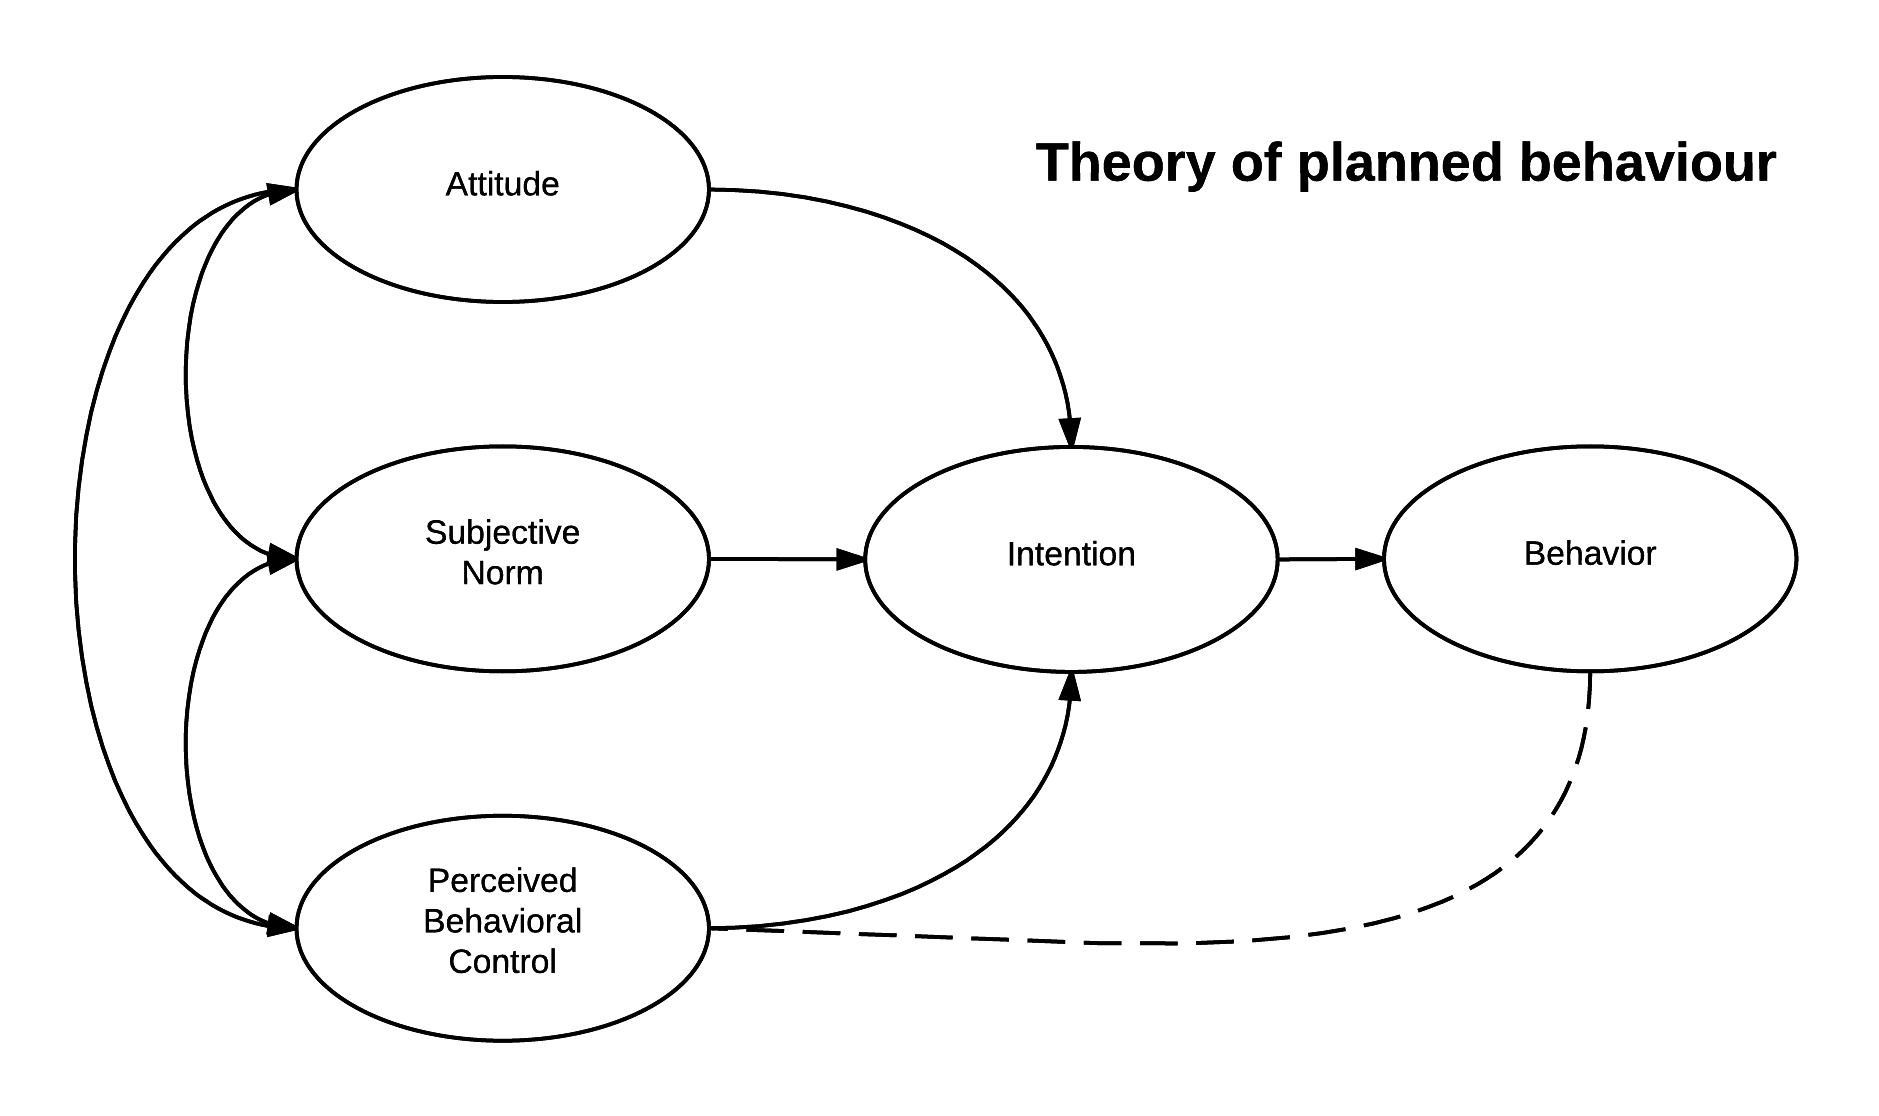
\includegraphics[width=0.8\textwidth]{Theory_of_planned_behavior_chart}}
    \caption{ساختار نظریه رفتار برنامه ریزی شده
      %\cite{kim2016integrated}
    }
    \label{fig:Theory_of_planned_behavior_chart}
  \end{figure}\\

  این نظریه در پژوهش‌های پیشین برای بررسی رفتار
  به اشتراک گذاری داده های خصوصی
  فرد در شبکه اجتماعی فیسبوک استفاده شده است
  \!\cite{vanderschyffInformationPrivacyBehavior2020}
  \!.
  مدلی که
  \!\gls{Theory of planned behavior}
  ارائه پیشنهاد می‌دهد، احتمال وقوع  رفتار‌های ارادی مخصوصا رفتار‌های ارادی مثبت به شدت تمایل فرد به
  انجام آن رفتار بستگی دارد.
  \!({\gls{Icek Ajzen}})
  عامل تعیین کننده برای انجام یک کار تمایلات او است.
\fi
%%%%%%%%%%%%%%%%%%%%

\ifSurveyfillingBehavior
  % بررسی اینکه آیا از نحوه پر کردن فرم ها می توان به کانفیدنس صداقت آزمودنی پی برد یا نه
  در صورتیکه گزینه‌های پرسشنامه اجباری باشند کیفیت داده‌های جمع‌آوری شده کاهش می یابد.
  \!\cite{sischkaImpactForcedAnswering2022}
\fi
% ^ %%%%%%%%%%%%%%%%%%%%%%%%%%%%%%%%%%%%%%%%%%%%%%%%%%%%%%%%%%%%%
% ^ %%%%%%%%%%%%%%%%%%%%%%%%%%%%%%%%%%%%%%%%%%%%%%%%%%%%%%%%%%%%%
% ^ %%%%%%%%%%%%%%%%%%%%%%%%%%%%%%%%%%%%%%%%%%%%%%%%%%%%%%%%%%%%%
\section{اهمیت}
%% توضیح بیشتر اضافه گردد بعدا
پژوهش انجام شده در سال ۲۰۲۰ نشان می دهد که در بازار داده های خصوصی آنلاین بازیگران زیادی به عنوان واسطه وجود دارند.
\!\cite{agogoInvisibleMarketOnline2021}
همچنین با گسترش هر روزه سیستم های اطلاعاتی که به
جمع‌آوری، ذخیره‌سازی، پردازش و به‌اشتراک‌گذاری داده‌های
خصوصی افراد می‌پردازند بررسی فرایندهای
تصمیم گیری و پارامتر‌های تاثیر گذار
بر این تصمیم‌گیری دارای اهمیت شده است
\!.
\!\cite{spiekermannValuesEthicsInformation2022}
از سوی دیگر نگرش افراد تصمیم گیرنده نسبت به ارزش اطلاعات خصوصی افراد می تواند نقش مهمی در رفتار آنها داشته باشد.
پژوهش‌هایی برای اندازه‌گیری ارزش داده‌های خصوصی انجام شده است
\!\cite{  fastValuePersonalData2021a,wesselsSellNotSell2019,tangHowChineseWeb2021}
\ifWillingnessToPay
  مقایسه میان رفتار افراد در پژوهش‌های اندازه‌گیری
  \textit{تمایل به پرداخت}
  \LTRfootnote{willingness to pay}
  نشان داده است که
  \textit{تمایل به پرداخت }
  با استفاده از روش‌های فرضی مانند
  \textit{ارزشيابی مشروط}
  \LTRfootnote{contingent valuation }
  میان ۱۷ تا ۶۳ درصد بالاتر
  از روشهای غیر فرضی مانند
  \textit{حراج تجربی}
  \LTRfootnote{experimental auction}
  است.
  حراج تجربی به عنوان یک روش
  \textit{سازگار با انگیزه}
  \LTRfootnote{incentive compatibility}
  شناسایی شده‌است
  \!\citep{martinez-carrascoComparingHypotheticalNonhypothetical2015}
  .
  یک فرایند،
  \textit{سازگار با انگیزه}
  است وقتی‌که همه شرکت‌کنندگان فقط  با درنظر گرفتن ترجیهات واقعی خود، بهترین خروجی را بدست می‌آورند
  \!\citep{nisanAlgorithmicGameTheory2007}
  \!.


\fi
% ^ %%%%%%%%%%%%%%%%%%%%%%%%%%%%%%%%%%%%%%%%%%%%%%%%%%%%%%%%%%%%%
% ^ %%%%%%%%%%%%%%%%%%%%%%%%%%%%%%%%%%%%%%%%%%%%%%%%%%%%%%%%%%%%%
% ^ %%%%%%%%%%%%%%%%%%%%%%%%%%%%%%%%%%%%%%%%%%%%%%%%%%%%%%%%%%%%%

\section{فرضیه پژوهشی}

% ^ %%%%%%%%%%%%%%%%%%%%%%%%%%%%%%%%%%%%%%%%%%%%%%%%%%%%%%%%%%%%%
% ^ %%%%%%%%%%%%%%%%%%%%%%%%%%%%%%%%%%%%%%%%%%%%%%%%%%%%%%%%%%%%%
% ^ %%%%%%%%%%%%%%%%%%%%%%%%%%%%%%%%%%%%%%%%%%%%%%%%%%%%%%%%%%%%%

% کلیه فایل‌های لازم برای حروف‌چینی با کلاس فوق، داخل پوشه‌ای به نام
% \lr{tehran-thesis}
% قرار داده شده است. توجه داشته باشید که برای استفاده از این کلاس باید فونت‌های
% \lr{IRLotusICEE}
% و
% \lr{IRTitr}
% را داشته باشید (که همراه با این کلاس هست و نیاز به نصب نیست).
% قلم‌های
% \lr{IRLotusICEE}
% مستخرج از قلم‌های استاندارد
% \lr{IRLotus}
% شورای عالی اطلاع‌رسانی%
% \footnote{
% قلم‌های استاندارد
% \lr{IRFonts}
% از شورای عالی اطلاع‌رسانی، منطبق بر آخرین نسخه استاندارد یونیکد، استاندارد ملی ۶۲۱۹ و استاندارد
% \lr{Adobe Glyph Naming}
% هستند.
% }
% هستند که توسط دکتر بابایی‌زاده اصلاحاتی روی آنها صورت پذیرفته است: تبدیل صفر توپر به صفر توخالی (جهت تمایز بیشتر با نقطه) و اضافه شدن
% \textit{\textbf{حالت توپر و ایرانیک توأم}}،
% که این موارد در قلم‌های شورای عالی اطلاع‌رسانی وجود ندارد.

% \subsection{این همه فایل؟!}
% \label{muchFiles}
% از آنجایی که یک پایان‌نامه یا رساله، یک نوشته بلند محسوب می‌شود، لذا اگر همه تنظیمات و مطالب پایان‌نامه را داخل یک فایل قرار بدهیم، باعث شلوغی و سردرگمی می‌شود. به همین خاطر، قسمت‌های مختلف پایان‌نامه یا رساله  داخل فایل‌های جداگانه قرار گرفته است. مثلاً تنظیمات پایه‌ای کلاس داخل فایل
% \lr{tehran-thesis.cls}، 
% قسمت مشخصات فارسی پایان‌نامه داخل 
% \lr{faTitle.tex}،
% مطالب فصل اول داخل 
% \lr{chapter1.tex}
% و تنظیمات قابل تغییر توسط کاربر داخل 
% \lr{commands.tex}،
% قرار داده شده است.
% \textbf{
% 	فایل اصلی این مجموعه، فایل
% 	\lr{main.tex}
% 	می‌باشد.
% }
% % یعنی بعد از تغییر فایل‌های دیگر، برای دیدن نتیجه تغییرات، باید این فایل را اجرا کرد. بقیه فایل‌ها به این فایل، کمک می‌کنند تا بتوانیم خروجی کار را ببینیم.
% اگر به فایل 
% \lr{main.tex}
% دقت کنید، متوجه می‌شوید که قسمت‌های مختلف پایان‌نامه، توسط دستورهایی مانند 
% \lr{input}
% و
% \lr{include}
% به فایل اصلی، یعنی 
% \lr{main.tex}
% معرفی شده‌اند.
% با توجه به ساختار محتوایی دستورالعمل، در فایل
% \lr{main.tex}
% فرض شده که پایان‌نامه یا رساله شما، از ۵ فصل و تعدادی پیوست تشکیل شده است. با اینحال، شما می‌توانید به راحتی فصل‌ها و پیوست‌ها را با صلاحدید اساتید راهنما، کم و زیاد کنید. این کار، بسیار ساده است. فرض کنید بخواهید یک فصل دیگر هم به پایان‌نامه اضافه کنید. برای این کار، کافی است یک فایل با نام دلخواه مثلاً 
% \lr{chapter6}
% و با پسوند 
% \lr{.tex}
% بسازید و آن را داخل پوشه 
% \lr{tehran-thesis}
% قرار دهید و سپس این فایل را با دستور 
% \verb!\include{chapter6}!
% داخل فایل
% \lr{main.tex}
%  فراخوانی کنید.

% \subsection{از کجا شروع کنم؟}
% قبل از هر چیز، باید یک توزیع تِک مناسب مانند تک‌لایو
% \lr{(TeXLive)}
% را روی سیستم خود نصب کنید. تک‌لایو  را می‌توانید از 
%  \href{http://www.tug.org/texlive}{سایت رسمی آن}%
% \LTRfootnote{\lr{\url{http://www.tug.org/texlive}}}
%  دانلود کنید یا مستقیماً از مخازن توزیع لینوکس خود بگیرید (مثلاً در اوبونتو با دستور
% \LRE{\verb!sudo apt install texlive-full!}).
% برای نصب تک‌لایو و اجرای اسناد زی‌پرشین می‌توانید از
% \href{http://parsilatex.com/site/shop/}{دی‌وی‌دی مجموعه پارسی‌لاتک}%
% \LTRfootnote{\lr{\url{http://parsilatex.com/site/shop/}}}
% و فایل راهنمای موجود در آن هم کمک بگیرید.

% برای تایپ و پردازش اسناد لاتک باید از یک ویرایشگر مناسب استفاده کنید. ویرایشگرهای
% \lr{TeXWroks},
% \lr{TeXstudio},
% \lr{Texmaker}
% و
% \lr{BiDiTeXmaker}
% بدین منظور تولید شده‌اند. می‌توان ویرایش‌گر 
%  \href{https://bitbucket.org/srazi/biditexmaker3}{\lr{BiDiTeXmaker}}%
%  \LTRfootnote{\lr{\url{https://bitbucket.org/srazi/biditexmaker3}}}
% را که بویژه برای کار با زی‌پرشین و مطالب دوجهته بهبود یافته است، بهینه‌ترین ویرایشگر لاتک برای کار با اسناد فارسی عنوان کرد.

% حال اگر نوشتن \پ اولین تجربه شما از کار با لاتک است، توصیه می‌شود که یک‌بار به صورت اجمالی، کتاب «%
% \href{http://www.tug.ctan.org/tex-archive/info/lshort/persian/lshort.pdf}{مقدمه‌ای نه چندان کوتاه بر
% \lr{\LaTeXe}}%
% \LTRfootnote{\lr{\url{http://www.tug.ctan.org/tex-archive/info/lshort/persian/lshort.pdf}\hfill}}»
% ترجمه دکتر مهدی امیدعلی را مطالعه کنید. این کتاب، کتاب بسیار کاملی است که خیلی از نیازهای شما در ارتباط با حروف‌چینی را برطرف می‌کند.
% اگر تک لایو کامل را داشته باشید، این کتاب را هم دارید. کافیست در خط فرمان دستور زیر را بزنید:
% \begin{latin}
% 	\texttt{texdoc lshort-persian}
% \end{latin}
% اگر عجله دارید، برخی دستورات پایه‌ای مورد نیاز در پیوست \ref{app:latexIntro} بیان شده‌اند.

% بعد از موارد گفته شده، فایل 
% \lr{main.tex}
% و
% \lr{faTitle.tex}
% را باز کنید و مشخصات پایان‌نامه خود مثل نام، نام خانوادگی، عنوان پایان‌نامه و ... را جایگزین مشخصات موجود در فایل
% \lr{faTitle.tex}
%  کنید. نیازی نیست نگران چینش این مشخصات در فایل پی‌دی‌اف خروجی باشید، زیرا کلاس 
% \lr{tehran-thesis}
% همه این کارها را بطور خودکار برای شما انجام می‌دهد. در ضمن، موقع تغییر دادن دستورهای داخل فایل
% \lr{faTitle.tex}
%  کاملاً دقت کنید؛ این دستورها، خیلی حساس هستند و ممکن است با یک تغییر کوچک، موقع اجرا، خطا بگیرید. برای دیدن خروجی کار، فایل 
% \lr{faTitle.tex}
%  را 
% \lr{Save}
% (نه 
% \lr{Save As})
% کنید و بعد به فایل 
% \lr{main.tex}
% برگشته و آن را اجرا کنید%
% \footnote{
% 	البته فایلهای این مجموعه به گونه‌ای هستند که در
% 	\lr{TeXWorks} یا
% 	\lr{TeXstudio}
% 	بدون بازگشت به فایل اصلی، می‌توانید سند خود را اجرا کنید.
% }.
%  حال اگر می‌خواهید مشخصات انگلیسی \پ را هم عوض کنید، فایل 
% \lr{enTitle.tex}
% را باز کنید و مشخصات داخلش را تغییر دهید.
% %\RTLfootnote{
% %برای نوشتن پروژه کارشناسی، نیازی به وارد کردن مشخصات انگلیسی پروژه نیست. بنابراین، این مشخصات بطور خودکار، نادیده گرفته می‌شود.
% %}
% در اینجا هم برای دیدن خروجی باید این فایل را ذخیره کرده، بعد به فایل 
% \lr{main.tex}
% برگشته و آن را اجرا کرد.

% برای راحتی بیشتر، کلاس 
% \lr{tehran-thesis.cls}
% طوری طراحی شده است که کافی است فقط  یک‌بار مشخصات \پ را (در فایل‌های
% \lr{faTitle.tex}
% و
% \lr{enTitle.tex})
% وارد کنید و هر جای دیگر که این مشخصات لازم باشند، به طور خودکار درج می‌شوند. با این حال، اگر مایل بودید، می‌توانید تنظیمات موجود را تغییر دهید؛ گرچه، در صورتیکه کاربر مبتدی هستید و یا با ساختار فایل‌های  
% \lr{cls}
%  آشنایی ندارید، بهتر است به فایل 
% \lr{tehran-thesis.cls}
% دست نزنید.

% نکته دیگری که باید به آن توجه کنید این است که در قالب آماده شده، سه گزینه به نام‌های
% \lr{bsc}،
% \lr{msc}
% و
% \lr{phd}
% برای نوشتن پروژه، پایان‌نامه و رساله، در نظر گرفته شده است. بنابراین اگر قصد تایپ پروژهٔ کارشناسی، پایان‌نامهٔ کارشناسی ارشد یا رسالهٔ دکتری را دارید، به ترتیب باید از گزینه‌های
% \lr{bsc}،
% \lr{msc}
% و
% \lr{phd}
% در فایل 
% \lr{main.tex}
% استفاده کنید. با انتخاب هر کدام از این گزینه‌ها، تنظیمات مربوط به آنها به طور خودکار، اعمال می‌شود.


% \subsection[مطالب پایان‌نامه را چطور بنویسم؟]
% {مطالب \پ را چطور بنویسم؟}
% \subsubsection{نوشتن فصل‌ها}
% همان‌طور که در بخش \ref{muchFiles} گفته شد برای جلوگیری از شلوغی، قسمت‌های مختلف \پ از جمله فصل‌ها، در فایل‌های جداگانه‌ای قرار داده شده‌اند. 
% مثلاً اگر می‌خواهید مطالب فصل ۱ را تایپ کنید، باید فایل‌های 
% \lr{main.tex}
% و
% \lr{chapter1.tex}
% را باز کرده و مطالب خود را جایگزین محتویات داخل 
% \lr{chapter1.tex}
% نمایید. دقت شود که در ابتدای برخی فایلها دستوراتی نوشته شده است و از شما خواسته شده که آن دستورات را حذف نکنید.

%توجه کنید که همان‌طور که قبلاً هم گفته شد، تنها فایل قابل اجرا، 
%\lr{main.tex}
%است. لذا برای دیدن حاصل (خروجی) فایل خود، باید  
%\lr{chapter1.tex}
%را ذخیره کرده و سپس فایل 
%\lr{main.tex}
%را اجرا کنید.

% نکته بسیار مهمی که در اینجا باید گفته شود این است که سیستم \lr{\TeX}، محتویات یک فایل تِک را به ترتیب پردازش می‌کند.  بنابراین، اگر مثلاً  دو فصل اول خود را نوشته و خروجی آنها را دیده‌اید و مشغول تایپ مطالب فصل ۳ هستید، بهتر است
% که دو دستور 
% \verb!% !TeX root=main.tex
% دستور زیر باعث شماره‌بندی صفحات فصول از ۱ می‌شود و باید در اولین فصل شما باشد. آن را حذف نکنید!
\pagenumbering{arabic} % 1, 2, ...

\chapter{مقدمه}
% دستور زیر باعث عدم‌نمایش شماره صفحه در اولین صفحه‌ی این فصل می‌شود.
%\thispagestyle{empty}
\ifDataveillance
  \textit{کریستین فوکس}
  \LTRfootnote{Christian Fuchs}
  جامعه شناس اتریشی،
  \textit{
    \gls{Social networking service}
  }
  \!({\lr{SNS}})
  در دنیای مدرن را به یک
  \textit{
    \gls{Panopticon}
  }
  تشبیه می کند   که در آن شرکت‌های بزرگی مانند
  \textit{
    \gls{Alphabet}
  }
  \!(
  شرکت مادر سرویس
  \textit{
    \gls{Google}
  }
  \!)
  و
  \textit{
    \gls{Meta}
  }
  \!(
  \!شرکت مادر و مالک برنامه‌های نرم‌افزاری مانند
  \textit{
    \gls{Instagram}
  }،
  \textit{
    \gls{Facebook}
  }
  و
  \textit{
    \gls{Whatsapp}
  }
  \!)
  به
  \textit{
    \gls{Dataveillance}
  }
  اعضا می‌پردازند
  \!\citep{romelePanopticismNotEnough2017a}.
  عبارت
  \textit{
    \gls{Panopticon}
  }
  را اولین بار
  \textit{
    \gls{Jeremy Bentham}
  }
  \!
  \citep{benthamPanopticonInspectionHouseContaining1791}
  برای توصیف ساختار‌های اجتماعی که مانند سیستم متمرکز نظارت عمل می‌کنند، از معماری وارد
  \textit{
    \gls{Social philosophy}
  }
  کرد.
\fi %Dataveillance
% * from old proposal and thesis fron khordad 1400 /media/d_drive/PJ/K/C/PJ-HDD-NiliLab/ssd2-laptop-backup-4mordad00/PJ/KN/Cog/proposal/tex/003
به نظر می‌رسد تصمیم‌گیرندگانی که در چنین سازمان‌هایی حضور دارند به حجم زیادی از اطلاعات
شخصی افراد دسترسی دارند. چنین افرادی، به علت وظیفه‌ای که در قبال سازمان
متبوع خود دارند، ملزم با حداکثر کردن سود بنگاه‌های اقتصادی هستند
که مالکیت این سازمان‌ها و سرویس‌های ارائه شده را، در اختیار
دارند.از طرف دیگر، همین تصمیمات می‌تواند باعث متضرر شدن
کاربرانی باشد که مالک اصلی اطلاعات جمع‌آوری شده می‌باشند. در چنین شرایطی، وقتی که
\textit{
  \glspl{Oversight institution}
}
با تغییرات سریع  در ساختارهای
\textit{
  \glspl{Information society}
}
ناهماهنگ هستند
\!\citep{cavoukianDiscussionPaperPrivacy2009,machovaDiscourseSurveillancePrivacy2021}،
بررسی ساز و کار موثر بر تصمیمات این افراد، اهمیت پیدا می‌کند.
اهمیت  این موضوع زمانی بیشتر می‌شود که کاربران
\textit{
  \gls{Social networking service}
}
تحت تاثیر
\textit{
  \glspl{Motivitions of}
}
متضاد قرار می‌گیرند و رفتاری را نشان می‌دهند که با عنوان
\textit{
  \gls{Privacy paradox}
}
شناخته می‌شود
\!citep{barthPrivacyParadoxInvestigating2017}.

این رفتار زمانی مشاهده می‌شود که کاربران شبکه‌های اجتماعی با وجود اهمیتی که برای حفظ
\textit{
  \gls{Information privacy}
}
بیان می‌کنند باز هم بی‌محابا نسبت به  منتشر کردن اطلاعات شخصی خود
در شبکه‌های اجتماعی اقدام می‌کنند.

این رفتار حتی پس از آگاه شدن از
پیامدهای سوءاستفاده از این اطلاعات نیز کاهش چشمگیری نداشته است
\!\citep{hermesWhoQuitsPrivacyInvasive2021,wirthLazinessExplanationPrivacy2022}.
به نظر می‌رسد که جلوگیری از پیامدهای  نامطلوب سوءاستفاده از اطلاعات خصوصی کاربران و نقض
\textit{
  \gls{Information privacy}
}
از طریق مداخلاتی که در سطح کاربران انجام شود، با توجه به گسترش و تنوع جمعیتی،
دشوار خواهد بود. با این وجود،
\textit{
  \gls{Information privacy}
}
که به توانایی افراد
برای کنترل اطلاعات مربوط به آنها اشاره دارد
\!{\cite{smithInformationPrivacyMeasuring1996}}
در سال‌های اخیر بیشتر مورد توجه کاربرانی قرار گرفته است
که داده‌های آنها توسط
\textit{
  \glspl{Social networking service}
}
جمع‌آوری، طبقه‌بندی و تحلیل می شود
\!{\cite{wallOrganizationalViolationsExternally2016}}
\!.
\textit{
  \gls{Information privacy}
}
با اشتراک‌گذاری اطلاعات شخصی توسط صاحب اطلاعات، در تضاد نیست.
\textit{
  \gls{Information privacy}
}
داشتن کنترل بر روی اطلاعات بعد از به  اشتراک‌گذاری، می‌باشد.
\!{\cite{acquistiEconomicsPrivacy2016}}.
به اشتراک گذاری اطلاعات شخصی از دید صاحبان اولیه اطلاعات،
به عنوان یک رفتار اجتماعی ناخوشایند و بالقوه ناهنجار، شناسایی شده است،
\!{\cite{norbergCopingInformationRequests2014}}،
اما به نظر می‌رسد چنین دیدگاهی با تعریفی که برای
\textit{
  \gls{Information privacy}
}
ارائه شد، در تضاد قرار می‌گیرد. اگر کاربران بتوانند بعد از
\textit{
  \gls{Disclosure}
}
اطلاعات خود، بر روی نحوه استفاده از آن کنترل داشته باشند،
\textit{
  \gls{Personal Information Sharing Behavior}
}
به تنهایی
اثرات مخربی در پی نخواهد داشت.  به علاوه
جمع‌آوری و پردازش اطلاعات می‌تواند نتایج سازنده‌ای، در سطح
اجتماعی و فردی داشته باشد
\!\citep{rockenbachProvidingPersonalInformation2020}.
افرادی که در
\textit{
  \glspl{Information society}
}
فاقد
\textit{
  \glspl{information record}
}
کافی در
\textit{
  \gls{Big data}
}
باشند، از جهات مختلف مورد
\textit{
  \gls{Discrimination}
}
قرار می‌گیرند
\!\citep{favarettoBigDataDiscrimination2019,lermanBigDataIts2013}.
با این دیدگاه، به اشتراک گذاری اطلاعات شخصی توسط صاحب اطلاعات، نه تنها
ناسازگارانه نیست، بلکه به یک رفتار
\textit{
  \gls{Prosocial}
}
تبدیل می‌شود. اطلاعات کاربران پس از
\textit{
  \gls{Disclosure}
}
در اختیار تصمیم‌گیرندگانی قرار می‌گیرد که در
\textit{
  \glspl{Social networking service}
}
مسئول جمع‌آوری، ذخیره‌سازی و پردازش اطلاعات هستند. به نظر می‌آید که حفظ
\textit{
  \gls{Information privacy}
}
و جلوگیری از اثرات مخرب اجتماعی و فردی سوءاستفاده از
اطلاعات شخصی انباشته شده، از طریق شناسایی عوامل موثر
بر تصمیم‌گیری این افراد و به اجرا در آوردن
مداخلات موثر در این سطح،نتایج بهتری در پی داشته باشد.

کاربران
\textit{
  \glspl{Social networking service}
}
پس از ارائه اطلاعات شخصی خود، خدماتی را از آن دریافت می‌کنند. این
تبادل میان کاربر و
\textit{
  \glspl{Social networking service}
}
مورد توافق طرفین است. شرایط حاکم بر این تبادل در توافق‌نامه‌ای
که در زمان عضویت به افراد ارائه می‌شود، مشخص شده است. به عنوان مثال
فرد در قبال اطلاعات شخصی خود از امکانات
\textit{
  \glspl{Social networking service}
}
برای برقراری ارتباط با دوستان خود استفاده می کند. او همچنین
با شروط دیگری که  برای عضویت لازم بوده است، موافقت کرده است. او
قبول کرده است که
\textit{
  \gls{Social networking service}
}
اطلاعات شخصی‌اش را در جهت ارائه تبلیغات هدفمند به کاربران، ذخیره کند
و مورد بازبینی و پردازش قرار دهد. اثرات مخرب این تبادل از زمانی شروع می شود که دریافت کننده اطلاعات، از
آن برای اهدافی به غیر از توافق اولیه استفاده کند و یا امکان این کار را برای یک شخص ثالث فراهم کند
\!{\cite{padyabExploringImpactsSecondary2018}}.

\textit{
  \gls{Secondary use of information}
}،
استفاده از اطلاعات شخصی برای اهدافی فراتر
از توافق اولیه، بعد از
\textit{
  \gls{Disclosure}
}
اطلاعات شخصی فرد، است. این عمل توسط موسسه جمع‌آوری کننده اطلاعات
و افراد تصمیم‌گیرنده در آن انجام می‌گیرد
\!{\cite{culnanHowDidThey1993}}.
پیامد‌های زیانبار تصمیمات بنگاه‌های اقتصادی و فن‌آوری بزرگی
مانند
\textit{
  \glspl{Meta}
}
برای استفاده ثانویه از اطلاعات شخصی جمع‌آوری شده، در پژوهش‌های مختلف بررسی شده اند
\!{\cite{padyabExploringImpactsSecondary2018}}.
این تصمیمات در سال‌های ۲۰۱۵ تا ۲۰۱۸، منجر به ناهنجاری‌های وسیع در سطح جوامع شدند
\!{\cite{redmanDataCredibilityProblem2013,dezwartSurveillanceBigData2014,spiekermannNetworksControlReport2016,schyffDuplicitouslMedia2020}}.
پیامدهای این ناهنجاری‌ها در نهایت افراد عضو جوامع را به طور غیر مستقیم
تحت تاثیر قرار می‌دهند. این افراد، متشکل از همان کاربرانی هستند که به طور جمعی، تامین کننده
داده‌های جمع‌آوری شده توسط
\textit{
  \glspl{Meta}
}
بوده‌اند.
\!{\cite{redmanDataCredibilityProblem2013,dezwartSurveillanceBigData2014,spiekermannNetworksControlReport2016,schyffDuplicitouslMedia2020}}.
با وجود آسیب‌پذیری افراد از داده‌های شخصی جمع‌آوری شده توسط شرکت‌ها
و شرکای تجاری آنها، تحقیقات نشان می‌دهد
که کاربران این جنبه تبادل اطلاعات خود را نادیده می‌گیرند
\!{\cite{raynes-goldieAliasesCreepingWall2010,brandtzaegTooManyFacebook2010,youngPrivacyProtectionStrategies2013}}،
هرچند با توجه به تاثیرات سازنده‌ای که برای رفتار اشتراک گذاری اطلاعات در بخش‌های
قبلی نام برده شده است، به نظر می‌رسد که می‌توان، تغییرات نامحسوس رفتار کاربران در
\textit{
  \gls{post–Cambridge Analytica scandal era}
}
\!{\citep{epsteinViewFramingDigital2021}}
را، پدیده مطلوبی توصیف کرد. با این وجود وقوع چنین پدیده‌هایی به 
\textit{
  \gls{Trust}
}
 در افراد جامعه آسیب می‌زند و در نهایت سبب کاهش منافع جمعیِ جمع‌آوری و پردازش اطلاعات، می‌گردد.


\gls{Cambridge Analytica scandal}
در سال ۲۰۱۶ باعث پی‌گیری‌ حقوقی شرکت 
\glspl{Meta} 
و مدیرعامل آن 
\textit{
  \gls{Mark Zuckerberg}
}
و محکومیت به پرداخت جریمه پنج میلیارد دلاری، شد
.\!{\citep{daviesFacebookPay5bn2019m,FacebookAgreesPay2019}}
واکنش مسؤولین فیسبوک نشان می‌دهد
که افراد تصمیم گیرنده در شرکت‌های جمع‌آوری کننده
اطلاعات نیز احتمالا از پیامدهایی که سیاست‌گذاری‌های آنها در استفاده ثانویه از اطلاعات شخصی کاربران
برای خود شرکت در پی دارد، ناآگاه هستند
\!{\cite{SuspendingCambridgeAnalytica2018,FacebookDataPrivacy2018}}
\!. با توجه به اینکه این افراد مسؤول حداکثر
کردن سود شرکت‌های خود هستند،
به نظر می‌رسد که چنین تصمیماتی فرض
\glspl{Rational}
بودن عامل‌های تصمیم‌گیرنده را در
\glspl{Rational choice theory}
به چالش می‌کشد. با در نظر گرفتن این مساله‌، ما در این پژوهش از از یک چارچوب نظری که فرض
\textit{
  \gls{Rational}
}
بودن تصمیمات را به چالش می‌کشند برای
\textit{
  \glspl{Articulation}
}
مفاهیم و رویکردهایمان استفاده کردیم.


تحقیقات زیادی برای بررسی رفتار کسانی که
اطلاعات خود را در اینترنت به اشتراک می‌گذارند انجام شده است
\!\!{\cite{kamleitnerInformationSharingPrivacy2019,kamleitnerYourDataMy2019}}.
همچنین رفتار افرادی که در مالکیت اطلاعت با فرد دیگر، شریک هستند بررسی شده است
\!\!{\cite{tawnieInterdependentPrivacy2017}}.
نتایج نشان می‌دهد که با وجود اینکه در همه جهان
\!،
\textit{
  \gls{Privacy}
}
اطلاعات شخصی افراد مساله مهمی برای کاربران آنلاین
است، بیشتر کاربران به ندرت برای محافظت از این داده، به خود زحمت می‌دهند و حتی در
بیشتر مواقع به طور داوطلبانه آن‌را پخش می‌کنند. تلاش زیادی انجام شده است تا این
دوگانگی میان
\textit{
  \gls{Privacy Attitude}
}
و رفتار، که معمولا با عنوان
\textit{
  \gls{Privacy paradox}
}
شناخته می‌شود، توضیح داده شود
\!\!{\cite{gerberExplainingPrivacyParadox2018}}.
به طور مشابه پژوهشی که در زمینه رفتار
\textit{
  \gls{Trust}
}
با به کار بردن
\textit{
  \gls{Theory of planned behavior}
}
در
\textit{
  \gls{Trust game}
}
انجام شده است،  وجود چنین تناقضی را در افراد
\textit{
  \gls{Trustor}
}
نیز نشان می‌دهد
\!\cite{gazdagNotWantTrust2019}.
به طور کلی، تا کنون  تحقیقات زیادی در حوزه
\textit{
  \gls{Information privacy}
}،
از
\textit{
  \gls{Trust game}
}
برای بررسی رفتار افراد در این تعامل
\textit{
  \gls{Interpersonal}
}،
استفاده کرده اند. با وجود اینکه تا به امروز رفتار کاربرانی که اطلاعات
\!(یا اطلاعات مشترک)
خود را به اشتراک می‌گذارند، مورد کنکاش قرار گرفته است، حیطه
رفتاری افرادی که دریافت کننده این  اطلاعات هستند به ندرت
مورد توجه قرار گرفته است
\!\cite{demmersYourDataAre2021}.

\subsection{کمبریج آنالیتیکا و استفاده ثانویه از اطلاعات}
در سال ۲۰۱۳ استاد دانشگاه کمبریج یک برنامه به نام 
«\lr{thisisyourdigitallife}»
ساخت. این برنامه در شبکه اجتماعی فیسبوک به کاربران 
آزمون‌های شخصیت‌شناسی ارائه می‌کرد. وقتی کاربر فیسبوک برنامه را بر روی حساب کاربری خود فعال و نصب
می‌کرد، برنامه جمع‌آوری اطلاعات شخصی او را آغاز می‌کرد. این اطلاعات شامل اطلاعات حساب کاربری و فعالیت‌های کاربر در فیسبوک
بود. فعالیت‌هایی مانند اینکه کاربر کدام محتوای فیسبوک را لایک کرده است. در حدود سیصد هزار نفر این 
برنامه را نصب کردند. اما اطلاعاتی که جمع‌آوری شد به این تعداد محدود نماند.  
این برنامه اطلاعاتی درباره دوستان کاربر که تنظیمات حریم خصوصی خود را درست  تنظیم نکرده بودند، را 
نیز جمع‌آوری کرد. در نتیجه برنامه توانست اطلاعات ۸۷ میلیون نفر را جمع‌آوری کند
\!\cite{kangFacebookSaysCambridge}.

سپس دکتر کوگان داده چمع‌آوری شده را به شرکت 
\textit{
  \gls{ Strategic Communication Laboratories (SCL)}
}
که مالک شرکت کمبریج آنالیتیکا است، انتقال داد. این شرکت یک موسسه مشاوره
سیاسی بود که از داده برای شناسایی ویژگی‌های شخصیتی و رفتار رای دهندگان
استفاده می‌کرد
\!\cite{rosenbergHowTrumpConsultants2018}. 
این شرکت از این داده برای کمک به به پویش محافظه‌کاران برای هدف
قرار دادن تبلیغات اینترنتی و پیام رسان‌ها استفاده کرد. این همان عملی 
بود که دکتر کوان شرایط و مقررات فیبوک را نقض کرد که انتقال یا 
فروش داده به هر شبکه تبلیغاتی ، دلال داده یا هر سرویس تبلیغاتی 
و درآمد‌زایی، ممنوع می‌کرد
\!\cite{granvilleFacebookCambridgeAnalytica2018}. 

وقتی در سال ۲۰۱۵ فیسبوک از این موضوع مطلع شد، برنامه دکتر کوگان 
را حذف  کرد و از کوگان و کمبریج آنالیتیکا درخواست کرد که
مدرکی ارائه دهند، که داده را پاک کرده‌اند. کوگان و کمبریج آنالیتیکا
به فیسبوک تاییده‌ای ارائه دادند که داده را حذف کرده‌اند. هرچند  کپی داده
خارج از کنترل فیسبوک باقی ماند.  وقتی الکساندر نیکس، مدیر عامل
کمبریج آنالیتیکا، به قانون‌گذاران گفت که شرکتش داده‌های فیسبوک را در
اختیار ندارد، یکی از کارمندان گفت که او اخیرا صدها گیگابایت داده را
بر روی سرورهای کمبریج آنالیتیکا دیده‌است و اطلاعات رمز نگاری نشده بودند.

در سال ۲۰۱۵، فیسبوک هیچ بیانیه عمومی‌ای درباره این رخداد منتشر نکرد. همچنین
کاربرانی که اطلاعات‌شان با کمبریج آنالیتیکا به اشتراک گذاشته شده 
بود. همچنین فیسبوک به کمیته تجارت فدرال، درباره این موضوع
چیزی نگفت. بر اساس آنچه که مارک زاکربرگ در کنفرانس دو روزه
 استماع‌اش در نهم و دهم آوریل ۲۰۱۸ گفت، به محض اینکه گواهی کمبریج آنالیتیکا
 مبنی بر حذف و تعهد عدم استفاده از داده را دریافت کردند، فیسبوک
 موضوع را خاتمه یافته تلقی کرد
 \!\cite{spanFacebookCEOMark}. 

 با منتشر شن این داستان در مارس ۲۰۱۸ در دو نشریه بین‌المللی، فیسبوک
 مطلع شد که داده تا آن روز پاک نشده بوده است. نتایج به بار آمده
 چنین حادثه‌ای بی سابقه بود. فیسبوک توسط چند نهاد قضایی در ایالت متحده، 
 جزیره انگلستان و اتحادیه اروپا مورد بازخواست قضایی قرار گرفت. یک پویش
 فیسبوک را حذف کنید راه افتاد و افت شدید قیمت سهام باعث شد تقریبا پنجاه میلیارد دلار
 سرمایه شرکت در عرض سه روز پس از فاش شدن اخبار، از بین رفت.




%   \glspl{phenomenon of dyadic completion}
%   نشان می دهد که گرایش های
%   \glspl{deontological}
%   و
%   \glspl{utilitarian}
%   نه تنها به طور همزمان فعال هستند
%   بلکه اغلب سازگار و تقویت کننده می‌باشند
%   \!{\cite{grayTwoMindsVs2012}}.
\subsection{چارچوب‌های نظری}
\textit{
  \gls{Rational choice theory}
}
\!{\cite{beckerEconomicApproachHuman1978}}،
این فرض را بنا می‌نهد که انسان‌ها بر اساس
تابعی از مجموع منفعت، با کسر مجموع هزینه‌های یک تصمیم
یا مبادله و برای حداکثر کردن فایده  شخصی دست به عمل می‌زنند.

این موضوع پایه‌ای برای طرح نظریه
\textit{
  \gls{Theory of reasoned action}
}
توسط
\textit{
  \gls{Icek Ajzen}
}
و
\textit{
  \gls{Martin Fishbein}
}
در در دهه ۸۰ میلادی شد. این نظریات پیشنهاد می‌کنند که بین
\textit{
  \gls{Atteutude}
}
و رفتار رابطه وجود دارد
\!{\cite{ajzenPredictionGoaldirectedBehavior1986}}.
فهم رفتار اختیاری افراد به وسیله
بررسی انگیزه‌هایی که باعث اجرای یک عمل می شود، هدف اصلی این نظریه بود. این نظریه
بیان می کند که قصد اجرای یک عمل پیش‌بینی‌کننده اصلی انجام یا عدم ایجاد رفتار  است. به
علاوه پارامتر هنجاری
(هنجارهای اجتماعی که عمل را احاطه کرده‌اند)
در اجرا شدن یا نشدن عمل نقش بازی می کند
\!{\citep{HealthBehaviorTheory2015,doswellTestingTheoryReasoned2011,ajzenAttitudesAttitudeBehaviorRelation2000}}
.
اما تحقیقاتی که در قالب چارچوب‌های
\textit{
  \gls{Behavioral economics}
}
انجام شد، این فرض را مورد تردید قرار داده اند
\!\cite{henrichEconomicManCrosscultural2005}.
برای رفع کاستی‌های
\textit{
  \gls{Theory of reasoned action}
}
آیزن در سال ۱۹۹۱ 
\!\citep{ajzenTheoryPlannedBehavior1991}
\textit{
  \gls{Theory of planned behavior}
}
را مطرح کرد. به بیان این تئوری سه پارامتر اصلی
\textit{
  \gls{Attitude}
}
\!،
\textit{\gls{Subjective norm}}
و
\textit{\gls{Perceived Behavioral control}}
\!،
\textit{\glspl{Behavioral intention}}
افراد را شکل می‌بخشند. پایه تفکر
\textit{
  \gls{Theory of planned behavior}
}
این است که
\textit{
  \gls{Personal Information Sharing Behavior}
}
از تعامل
\textit{\glspl{Psychological construct}}
\textit{
  \gls{Attitude}
}
\!،
\textit{\gls{Subjective norm}}،
\textit{\gls{Perceived Behavioral control}}
و
\textit{\glspl{Behavioral intention}}
نسبت به 
\textit{
  \gls{Personal Information Sharing}
}،
ایجاد می‌شود. 

در پژوهش‌های پیشین برای بررسی
\textit{
  \gls{Personal Information Sharing Behavior}
}
از
\textit{
  \gls{Theory of reasoned action}
}
\!\citep{malhotraInternetUsersInformation2004}،
و
\textit{
  \gls{Theory of planned behavior}
}
برای ایجاد ساختاری که روابط بین پارامترها را مدل می‌کند، استفاده شده است
\!\citep{dinevExtendedPrivacyCalculus2006b}.

در این پژوهش ما بررسی رفتار به اشتراک گذاری اطلاعات خصوصی دیگران در
\textit{
  \gls{Conceptual framework}
}
\textit{
  \gls{Theory of planned behavior}
}
پرداختیم.

برای سنجش رویکرد‍ افراد به
\textit{
  \gls{Personal information of Others}
}
یک پرسشنامه بر اساس دسته‌بندی‌های هفت‌گانه‌ای که در پژوهش پیشین با توجه به رویکرد صاحبان
اولیه اطلاعات خصوصی نسبت به خطر فاش شدن اطلاعات شخصی شان در حوزه‌های مختلف، ساخته شد.
این پرسشنامه برای هر دسته از سوالات دارای ۲ سوال است. برای اینکه بتوان باور 
آزمودنی‌ها، را هم بر اساس ارزش ذهنی خود
\!(نگرش به ارزش اطلاعات)
و هم بر اساس ارزش ذهنی دیگران
\!(هنجار ذهنی و باور هنجاری)
و همچنین برای اندازه‌گیری پایایی درونی،
سوالات به دو دسته تقسیم ‌می‌شود.
به هر آزمودنی، دسته اول اطلاعات خصوصی به همراه یک سوال برای سنجش باور هنجاری، و دسته دوم
اطلاعات به همراه سوال دیگر برای سنجش باور شخصی، ارائه شد. به طور تصادفی این دو دسته از 
سوالات برای هر آزمودنی جابجا شدند تا در نهایت پاسخ‌های نیمی از آزمونی‌ها به دسته اول سوالات از دید خود و نیمی 
دیگر از آزمودنی ها به دسته دوم سوالات از دید خود، جمع‌آوری شوند. به همین ترتیب پاسخ به سوالات دسته اول و دوم 
با توجه به باور هنجاری از دو دسته مستقل به تصادف انتخاب شدند، جمع‌آوری شد. تصادفی سازی در زمان وردو آزمودنی‌ها
به آزمایش با انتصاب افراد با احتمال ۵۰ درصد به دو گروه، انجام شد.
% * %%%%%%%%%%%%%%%%%%%%%%%%%%%%%%%%%%%%%%%%%% from old proposal and thesis from khordad 1400

\section{متغیر‌ها و پرسشنامه‌ها}

\ifPlennedBahaviorTheory
  \textit{\gls{Theory of planned behavior}}
  \!(TPB)
  % \LTRfootnote{Theory of planned behavior (TPB) }
  %  acronyms اضافه شود
  ، تعامل سه باور فردی شامل
  \textit{\gls{Atteutude}} ،
  \textit{\gls{Subjective norm}} و
  \textit{\gls{Perceived Behavioral control}}
  % \LTRfootnote{Perceived Behavioral control}
  را عامل رفتار می داند
  \!(شکل: \ref{fig:Theory_of_planned_behavior_chart})
  \!\cite{ajzenTheoryPlannedBehavior2020}.
  در این نظریه 
  \textit{\gls{Atteutude}}
 از دو نگرش احساسی و نگرش ابزاری تشکیل شده است.
  \textit{\gls{Subjective norm}}
  شامل  هنجارهای ذهنی و هنجار توصیفی است.
  \textit{\gls{Perceived Behavioral control}}،
  دو بخش کنترل رفتاری درک شده و خود کارآمدی درک شده را شامل می باشد
  در این نظریه عامل اصلی تعیین کننده
  رفتار، قصد رفتاری است و اجزای ساختاری این نظریه
  بر روی قصد تاثیر ویژه‌ای دارند
  \cite{mhmdpwrBrrsyTthyrTywry2022}
  \begin{figure}[ht]
    \centerline{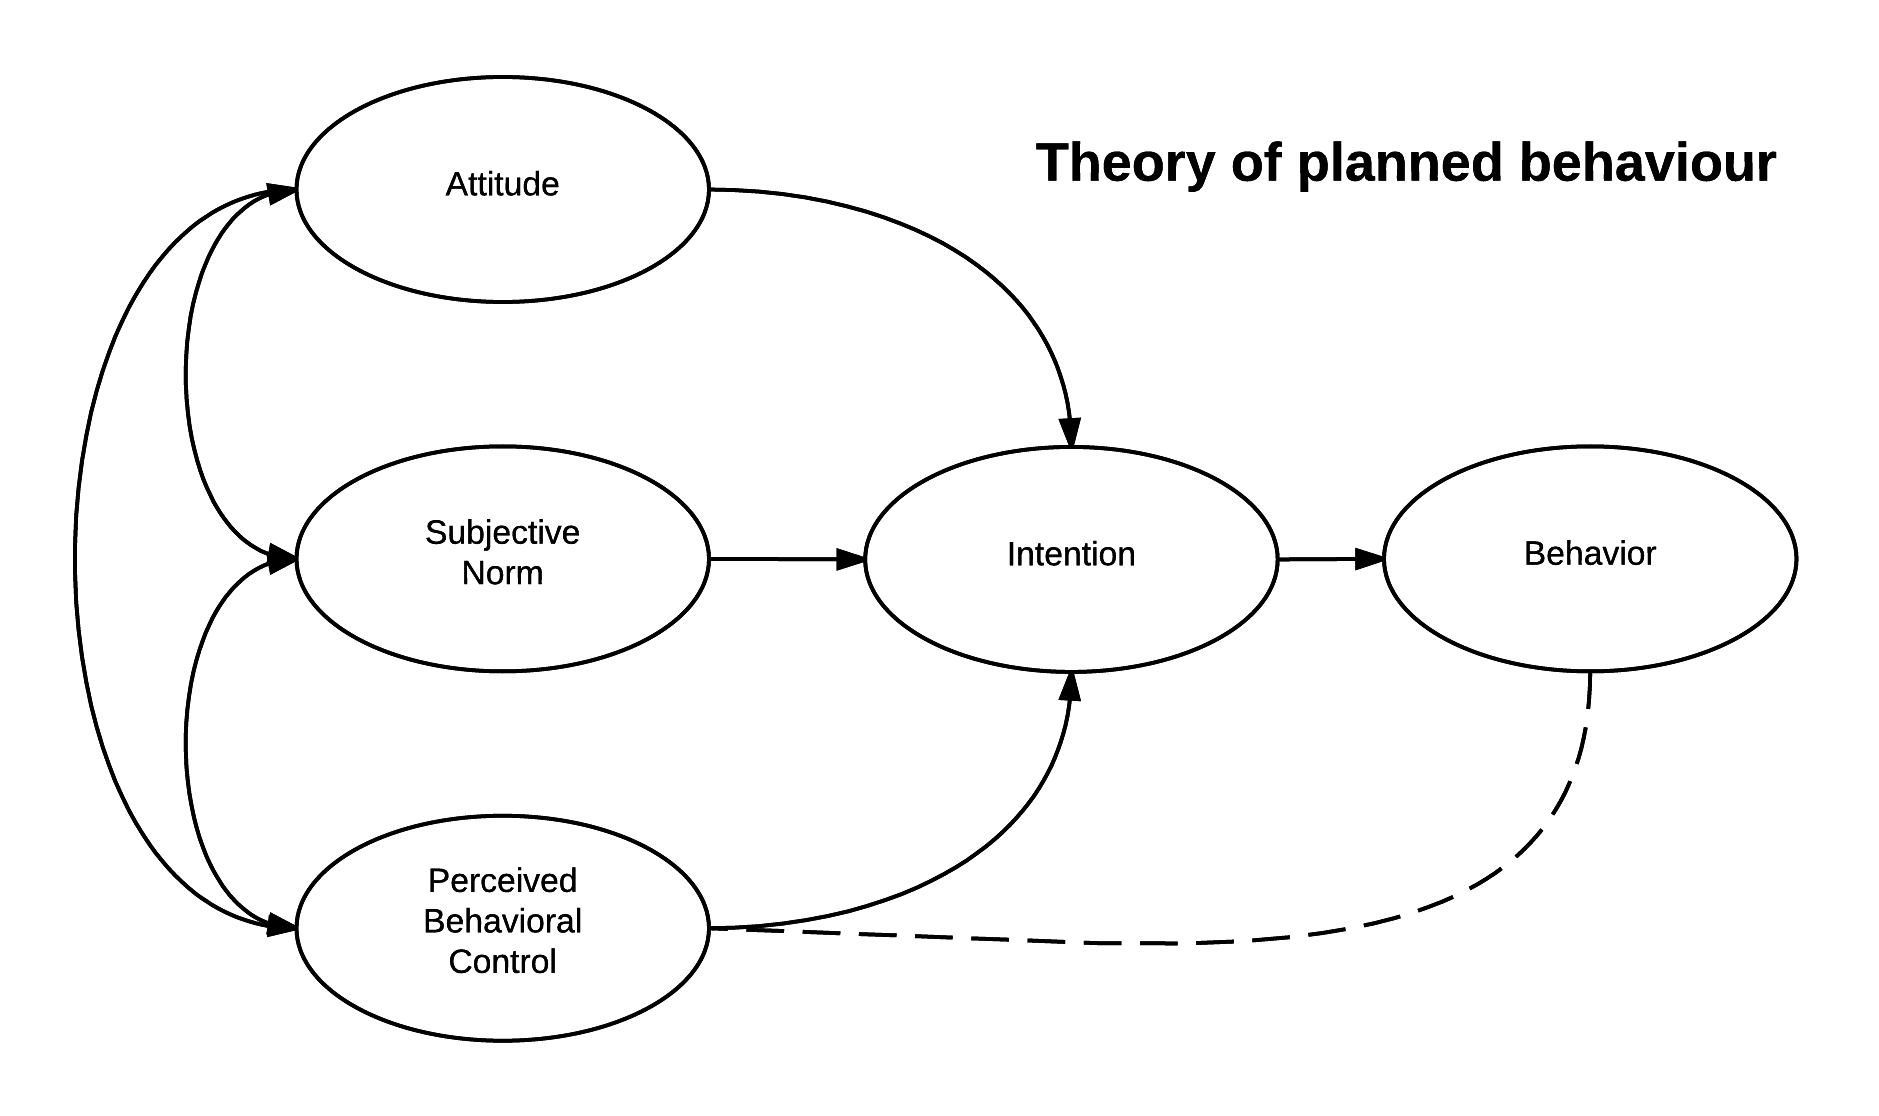
\includegraphics[width=0.8\textwidth]{Theory_of_planned_behavior_chart}}
    \caption{ساختار نظریه رفتار برنامه ریزی شده
      %\cite{kim2016integrated}
    }
    \label{fig:Theory_of_planned_behavior_chart}
  \end{figure}\\

  این نظریه در پژوهش‌های پیشین برای بررسی رفتار
  به اشتراک گذاری داده های خصوصی
  فرد در شبکه اجتماعی فیسبوک استفاده شده است
  \!\cite{vanderschyffInformationPrivacyBehavior2020}
  \!.
  مدلی که
  \!\gls{Theory of planned behavior}
  ارائه پیشنهاد می‌دهد، احتمال وقوع  رفتار‌های ارادی مخصوصا رفتار‌های ارادی مثبت به شدت تمایل فرد به
  انجام آن رفتار بستگی دارد.
  \!({\gls{Icek Ajzen}})
  عامل تعیین کننده برای انجام یک کار تمایلات او است.
\fi
%%%%%%%%%%%%%%%%%%%%

\ifSurveyfillingBehavior
  % بررسی اینکه آیا از نحوه پر کردن فرم ها می توان به کانفیدنس صداقت آزمودنی پی برد یا نه
  در صورتیکه گزینه‌های پرسشنامه اجباری باشند کیفیت داده‌های جمع‌آوری شده کاهش می یابد.
  \!\cite{sischkaImpactForcedAnswering2022}
\fi
% ^ %%%%%%%%%%%%%%%%%%%%%%%%%%%%%%%%%%%%%%%%%%%%%%%%%%%%%%%%%%%%%
% ^ %%%%%%%%%%%%%%%%%%%%%%%%%%%%%%%%%%%%%%%%%%%%%%%%%%%%%%%%%%%%%
% ^ %%%%%%%%%%%%%%%%%%%%%%%%%%%%%%%%%%%%%%%%%%%%%%%%%%%%%%%%%%%%%
\section{اهمیت}
%% توضیح بیشتر اضافه گردد بعدا
پژوهش انجام شده در سال ۲۰۲۰ نشان می دهد که در بازار داده های خصوصی آنلاین بازیگران زیادی به عنوان واسطه وجود دارند.
\!\cite{agogoInvisibleMarketOnline2021}
همچنین با گسترش هر روزه سیستم های اطلاعاتی که به
جمع‌آوری، ذخیره‌سازی، پردازش و به‌اشتراک‌گذاری داده‌های
خصوصی افراد می‌پردازند بررسی فرایندهای
تصمیم گیری و پارامتر‌های تاثیر گذار
بر این تصمیم‌گیری دارای اهمیت شده است
\!.
\!\cite{spiekermannValuesEthicsInformation2022}
از سوی دیگر نگرش افراد تصمیم گیرنده نسبت به ارزش اطلاعات خصوصی افراد می تواند نقش مهمی در رفتار آنها داشته باشد.
پژوهش‌هایی برای اندازه‌گیری ارزش داده‌های خصوصی انجام شده است
\!\cite{  fastValuePersonalData2021a,wesselsSellNotSell2019,tangHowChineseWeb2021}
\ifWillingnessToPay
  مقایسه میان رفتار افراد در پژوهش‌های اندازه‌گیری
  \textit{تمایل به پرداخت}
  \LTRfootnote{willingness to pay}
  نشان داده است که
  \textit{تمایل به پرداخت }
  با استفاده از روش‌های فرضی مانند
  \textit{ارزشيابی مشروط}
  \LTRfootnote{contingent valuation }
  میان ۱۷ تا ۶۳ درصد بالاتر
  از روشهای غیر فرضی مانند
  \textit{حراج تجربی}
  \LTRfootnote{experimental auction}
  است.
  حراج تجربی به عنوان یک روش
  \textit{سازگار با انگیزه}
  \LTRfootnote{incentive compatibility}
  شناسایی شده‌است
  \!\citep{martinez-carrascoComparingHypotheticalNonhypothetical2015}
  .
  یک فرایند،
  \textit{سازگار با انگیزه}
  است وقتی‌که همه شرکت‌کنندگان فقط  با درنظر گرفتن ترجیهات واقعی خود، بهترین خروجی را بدست می‌آورند
  \!\citep{nisanAlgorithmicGameTheory2007}
  \!.


\fi
% ^ %%%%%%%%%%%%%%%%%%%%%%%%%%%%%%%%%%%%%%%%%%%%%%%%%%%%%%%%%%%%%
% ^ %%%%%%%%%%%%%%%%%%%%%%%%%%%%%%%%%%%%%%%%%%%%%%%%%%%%%%%%%%%%%
% ^ %%%%%%%%%%%%%%%%%%%%%%%%%%%%%%%%%%%%%%%%%%%%%%%%%%%%%%%%%%%%%

\section{فرضیه پژوهشی}

% ^ %%%%%%%%%%%%%%%%%%%%%%%%%%%%%%%%%%%%%%%%%%%%%%%%%%%%%%%%%%%%%
% ^ %%%%%%%%%%%%%%%%%%%%%%%%%%%%%%%%%%%%%%%%%%%%%%%%%%%%%%%%%%%%%
% ^ %%%%%%%%%%%%%%%%%%%%%%%%%%%%%%%%%%%%%%%%%%%%%%%%%%%%%%%%%%%%%

% کلیه فایل‌های لازم برای حروف‌چینی با کلاس فوق، داخل پوشه‌ای به نام
% \lr{tehran-thesis}
% قرار داده شده است. توجه داشته باشید که برای استفاده از این کلاس باید فونت‌های
% \lr{IRLotusICEE}
% و
% \lr{IRTitr}
% را داشته باشید (که همراه با این کلاس هست و نیاز به نصب نیست).
% قلم‌های
% \lr{IRLotusICEE}
% مستخرج از قلم‌های استاندارد
% \lr{IRLotus}
% شورای عالی اطلاع‌رسانی%
% \footnote{
% قلم‌های استاندارد
% \lr{IRFonts}
% از شورای عالی اطلاع‌رسانی، منطبق بر آخرین نسخه استاندارد یونیکد، استاندارد ملی ۶۲۱۹ و استاندارد
% \lr{Adobe Glyph Naming}
% هستند.
% }
% هستند که توسط دکتر بابایی‌زاده اصلاحاتی روی آنها صورت پذیرفته است: تبدیل صفر توپر به صفر توخالی (جهت تمایز بیشتر با نقطه) و اضافه شدن
% \textit{\textbf{حالت توپر و ایرانیک توأم}}،
% که این موارد در قلم‌های شورای عالی اطلاع‌رسانی وجود ندارد.

% \subsection{این همه فایل؟!}
% \label{muchFiles}
% از آنجایی که یک پایان‌نامه یا رساله، یک نوشته بلند محسوب می‌شود، لذا اگر همه تنظیمات و مطالب پایان‌نامه را داخل یک فایل قرار بدهیم، باعث شلوغی و سردرگمی می‌شود. به همین خاطر، قسمت‌های مختلف پایان‌نامه یا رساله  داخل فایل‌های جداگانه قرار گرفته است. مثلاً تنظیمات پایه‌ای کلاس داخل فایل
% \lr{tehran-thesis.cls}، 
% قسمت مشخصات فارسی پایان‌نامه داخل 
% \lr{faTitle.tex}،
% مطالب فصل اول داخل 
% \lr{chapter1.tex}
% و تنظیمات قابل تغییر توسط کاربر داخل 
% \lr{commands.tex}،
% قرار داده شده است.
% \textbf{
% 	فایل اصلی این مجموعه، فایل
% 	\lr{main.tex}
% 	می‌باشد.
% }
% % یعنی بعد از تغییر فایل‌های دیگر، برای دیدن نتیجه تغییرات، باید این فایل را اجرا کرد. بقیه فایل‌ها به این فایل، کمک می‌کنند تا بتوانیم خروجی کار را ببینیم.
% اگر به فایل 
% \lr{main.tex}
% دقت کنید، متوجه می‌شوید که قسمت‌های مختلف پایان‌نامه، توسط دستورهایی مانند 
% \lr{input}
% و
% \lr{include}
% به فایل اصلی، یعنی 
% \lr{main.tex}
% معرفی شده‌اند.
% با توجه به ساختار محتوایی دستورالعمل، در فایل
% \lr{main.tex}
% فرض شده که پایان‌نامه یا رساله شما، از ۵ فصل و تعدادی پیوست تشکیل شده است. با اینحال، شما می‌توانید به راحتی فصل‌ها و پیوست‌ها را با صلاحدید اساتید راهنما، کم و زیاد کنید. این کار، بسیار ساده است. فرض کنید بخواهید یک فصل دیگر هم به پایان‌نامه اضافه کنید. برای این کار، کافی است یک فایل با نام دلخواه مثلاً 
% \lr{chapter6}
% و با پسوند 
% \lr{.tex}
% بسازید و آن را داخل پوشه 
% \lr{tehran-thesis}
% قرار دهید و سپس این فایل را با دستور 
% \verb!\include{chapter6}!
% داخل فایل
% \lr{main.tex}
%  فراخوانی کنید.

% \subsection{از کجا شروع کنم؟}
% قبل از هر چیز، باید یک توزیع تِک مناسب مانند تک‌لایو
% \lr{(TeXLive)}
% را روی سیستم خود نصب کنید. تک‌لایو  را می‌توانید از 
%  \href{http://www.tug.org/texlive}{سایت رسمی آن}%
% \LTRfootnote{\lr{\url{http://www.tug.org/texlive}}}
%  دانلود کنید یا مستقیماً از مخازن توزیع لینوکس خود بگیرید (مثلاً در اوبونتو با دستور
% \LRE{\verb!sudo apt install texlive-full!}).
% برای نصب تک‌لایو و اجرای اسناد زی‌پرشین می‌توانید از
% \href{http://parsilatex.com/site/shop/}{دی‌وی‌دی مجموعه پارسی‌لاتک}%
% \LTRfootnote{\lr{\url{http://parsilatex.com/site/shop/}}}
% و فایل راهنمای موجود در آن هم کمک بگیرید.

% برای تایپ و پردازش اسناد لاتک باید از یک ویرایشگر مناسب استفاده کنید. ویرایشگرهای
% \lr{TeXWroks},
% \lr{TeXstudio},
% \lr{Texmaker}
% و
% \lr{BiDiTeXmaker}
% بدین منظور تولید شده‌اند. می‌توان ویرایش‌گر 
%  \href{https://bitbucket.org/srazi/biditexmaker3}{\lr{BiDiTeXmaker}}%
%  \LTRfootnote{\lr{\url{https://bitbucket.org/srazi/biditexmaker3}}}
% را که بویژه برای کار با زی‌پرشین و مطالب دوجهته بهبود یافته است، بهینه‌ترین ویرایشگر لاتک برای کار با اسناد فارسی عنوان کرد.

% حال اگر نوشتن \پ اولین تجربه شما از کار با لاتک است، توصیه می‌شود که یک‌بار به صورت اجمالی، کتاب «%
% \href{http://www.tug.ctan.org/tex-archive/info/lshort/persian/lshort.pdf}{مقدمه‌ای نه چندان کوتاه بر
% \lr{\LaTeXe}}%
% \LTRfootnote{\lr{\url{http://www.tug.ctan.org/tex-archive/info/lshort/persian/lshort.pdf}\hfill}}»
% ترجمه دکتر مهدی امیدعلی را مطالعه کنید. این کتاب، کتاب بسیار کاملی است که خیلی از نیازهای شما در ارتباط با حروف‌چینی را برطرف می‌کند.
% اگر تک لایو کامل را داشته باشید، این کتاب را هم دارید. کافیست در خط فرمان دستور زیر را بزنید:
% \begin{latin}
% 	\texttt{texdoc lshort-persian}
% \end{latin}
% اگر عجله دارید، برخی دستورات پایه‌ای مورد نیاز در پیوست \ref{app:latexIntro} بیان شده‌اند.

% بعد از موارد گفته شده، فایل 
% \lr{main.tex}
% و
% \lr{faTitle.tex}
% را باز کنید و مشخصات پایان‌نامه خود مثل نام، نام خانوادگی، عنوان پایان‌نامه و ... را جایگزین مشخصات موجود در فایل
% \lr{faTitle.tex}
%  کنید. نیازی نیست نگران چینش این مشخصات در فایل پی‌دی‌اف خروجی باشید، زیرا کلاس 
% \lr{tehran-thesis}
% همه این کارها را بطور خودکار برای شما انجام می‌دهد. در ضمن، موقع تغییر دادن دستورهای داخل فایل
% \lr{faTitle.tex}
%  کاملاً دقت کنید؛ این دستورها، خیلی حساس هستند و ممکن است با یک تغییر کوچک، موقع اجرا، خطا بگیرید. برای دیدن خروجی کار، فایل 
% \lr{faTitle.tex}
%  را 
% \lr{Save}
% (نه 
% \lr{Save As})
% کنید و بعد به فایل 
% \lr{main.tex}
% برگشته و آن را اجرا کنید%
% \footnote{
% 	البته فایلهای این مجموعه به گونه‌ای هستند که در
% 	\lr{TeXWorks} یا
% 	\lr{TeXstudio}
% 	بدون بازگشت به فایل اصلی، می‌توانید سند خود را اجرا کنید.
% }.
%  حال اگر می‌خواهید مشخصات انگلیسی \پ را هم عوض کنید، فایل 
% \lr{enTitle.tex}
% را باز کنید و مشخصات داخلش را تغییر دهید.
% %\RTLfootnote{
% %برای نوشتن پروژه کارشناسی، نیازی به وارد کردن مشخصات انگلیسی پروژه نیست. بنابراین، این مشخصات بطور خودکار، نادیده گرفته می‌شود.
% %}
% در اینجا هم برای دیدن خروجی باید این فایل را ذخیره کرده، بعد به فایل 
% \lr{main.tex}
% برگشته و آن را اجرا کرد.

% برای راحتی بیشتر، کلاس 
% \lr{tehran-thesis.cls}
% طوری طراحی شده است که کافی است فقط  یک‌بار مشخصات \پ را (در فایل‌های
% \lr{faTitle.tex}
% و
% \lr{enTitle.tex})
% وارد کنید و هر جای دیگر که این مشخصات لازم باشند، به طور خودکار درج می‌شوند. با این حال، اگر مایل بودید، می‌توانید تنظیمات موجود را تغییر دهید؛ گرچه، در صورتیکه کاربر مبتدی هستید و یا با ساختار فایل‌های  
% \lr{cls}
%  آشنایی ندارید، بهتر است به فایل 
% \lr{tehran-thesis.cls}
% دست نزنید.

% نکته دیگری که باید به آن توجه کنید این است که در قالب آماده شده، سه گزینه به نام‌های
% \lr{bsc}،
% \lr{msc}
% و
% \lr{phd}
% برای نوشتن پروژه، پایان‌نامه و رساله، در نظر گرفته شده است. بنابراین اگر قصد تایپ پروژهٔ کارشناسی، پایان‌نامهٔ کارشناسی ارشد یا رسالهٔ دکتری را دارید، به ترتیب باید از گزینه‌های
% \lr{bsc}،
% \lr{msc}
% و
% \lr{phd}
% در فایل 
% \lr{main.tex}
% استفاده کنید. با انتخاب هر کدام از این گزینه‌ها، تنظیمات مربوط به آنها به طور خودکار، اعمال می‌شود.


% \subsection[مطالب پایان‌نامه را چطور بنویسم؟]
% {مطالب \پ را چطور بنویسم؟}
% \subsubsection{نوشتن فصل‌ها}
% همان‌طور که در بخش \ref{muchFiles} گفته شد برای جلوگیری از شلوغی، قسمت‌های مختلف \پ از جمله فصل‌ها، در فایل‌های جداگانه‌ای قرار داده شده‌اند. 
% مثلاً اگر می‌خواهید مطالب فصل ۱ را تایپ کنید، باید فایل‌های 
% \lr{main.tex}
% و
% \lr{chapter1.tex}
% را باز کرده و مطالب خود را جایگزین محتویات داخل 
% \lr{chapter1.tex}
% نمایید. دقت شود که در ابتدای برخی فایلها دستوراتی نوشته شده است و از شما خواسته شده که آن دستورات را حذف نکنید.

%توجه کنید که همان‌طور که قبلاً هم گفته شد، تنها فایل قابل اجرا، 
%\lr{main.tex}
%است. لذا برای دیدن حاصل (خروجی) فایل خود، باید  
%\lr{chapter1.tex}
%را ذخیره کرده و سپس فایل 
%\lr{main.tex}
%را اجرا کنید.

% نکته بسیار مهمی که در اینجا باید گفته شود این است که سیستم \lr{\TeX}، محتویات یک فایل تِک را به ترتیب پردازش می‌کند.  بنابراین، اگر مثلاً  دو فصل اول خود را نوشته و خروجی آنها را دیده‌اید و مشغول تایپ مطالب فصل ۳ هستید، بهتر است
% که دو دستور 
% \verb!% !TeX root=main.tex
% دستور زیر باعث شماره‌بندی صفحات فصول از ۱ می‌شود و باید در اولین فصل شما باشد. آن را حذف نکنید!
\pagenumbering{arabic} % 1, 2, ...

\chapter{مقدمه}
% دستور زیر باعث عدم‌نمایش شماره صفحه در اولین صفحه‌ی این فصل می‌شود.
%\thispagestyle{empty}
\ifDataveillance
  \textit{کریستین فوکس}
  \LTRfootnote{Christian Fuchs}
  جامعه شناس اتریشی،
  \textit{
    \gls{Social networking service}
  }
  \!({\lr{SNS}})
  در دنیای مدرن را به یک
  \textit{
    \gls{Panopticon}
  }
  تشبیه می کند   که در آن شرکت‌های بزرگی مانند
  \textit{
    \gls{Alphabet}
  }
  \!(
  شرکت مادر سرویس
  \textit{
    \gls{Google}
  }
  \!)
  و
  \textit{
    \gls{Meta}
  }
  \!(
  \!شرکت مادر و مالک برنامه‌های نرم‌افزاری مانند
  \textit{
    \gls{Instagram}
  }،
  \textit{
    \gls{Facebook}
  }
  و
  \textit{
    \gls{Whatsapp}
  }
  \!)
  به
  \textit{
    \gls{Dataveillance}
  }
  اعضا می‌پردازند
  \!\citep{romelePanopticismNotEnough2017a}.
  عبارت
  \textit{
    \gls{Panopticon}
  }
  را اولین بار
  \textit{
    \gls{Jeremy Bentham}
  }
  \!
  \citep{benthamPanopticonInspectionHouseContaining1791}
  برای توصیف ساختار‌های اجتماعی که مانند سیستم متمرکز نظارت عمل می‌کنند، از معماری وارد
  \textit{
    \gls{Social philosophy}
  }
  کرد.
\fi %Dataveillance
% * from old proposal and thesis fron khordad 1400 /media/d_drive/PJ/K/C/PJ-HDD-NiliLab/ssd2-laptop-backup-4mordad00/PJ/KN/Cog/proposal/tex/003
به نظر می‌رسد تصمیم‌گیرندگانی که در چنین سازمان‌هایی حضور دارند به حجم زیادی از اطلاعات
شخصی افراد دسترسی دارند. چنین افرادی، به علت وظیفه‌ای که در قبال سازمان
متبوع خود دارند، ملزم با حداکثر کردن سود بنگاه‌های اقتصادی هستند
که مالکیت این سازمان‌ها و سرویس‌های ارائه شده را، در اختیار
دارند.از طرف دیگر، همین تصمیمات می‌تواند باعث متضرر شدن
کاربرانی باشد که مالک اصلی اطلاعات جمع‌آوری شده می‌باشند. در چنین شرایطی، وقتی که
\textit{
  \glspl{Oversight institution}
}
با تغییرات سریع  در ساختارهای
\textit{
  \glspl{Information society}
}
ناهماهنگ هستند
\!\citep{cavoukianDiscussionPaperPrivacy2009,machovaDiscourseSurveillancePrivacy2021}،
بررسی ساز و کار موثر بر تصمیمات این افراد، اهمیت پیدا می‌کند.
اهمیت  این موضوع زمانی بیشتر می‌شود که کاربران
\textit{
  \gls{Social networking service}
}
تحت تاثیر
\textit{
  \glspl{Motivitions of}
}
متضاد قرار می‌گیرند و رفتاری را نشان می‌دهند که با عنوان
\textit{
  \gls{Privacy paradox}
}
شناخته می‌شود
\!citep{barthPrivacyParadoxInvestigating2017}.

این رفتار زمانی مشاهده می‌شود که کاربران شبکه‌های اجتماعی با وجود اهمیتی که برای حفظ
\textit{
  \gls{Information privacy}
}
بیان می‌کنند باز هم بی‌محابا نسبت به  منتشر کردن اطلاعات شخصی خود
در شبکه‌های اجتماعی اقدام می‌کنند.

این رفتار حتی پس از آگاه شدن از
پیامدهای سوءاستفاده از این اطلاعات نیز کاهش چشمگیری نداشته است
\!\citep{hermesWhoQuitsPrivacyInvasive2021,wirthLazinessExplanationPrivacy2022}.
به نظر می‌رسد که جلوگیری از پیامدهای  نامطلوب سوءاستفاده از اطلاعات خصوصی کاربران و نقض
\textit{
  \gls{Information privacy}
}
از طریق مداخلاتی که در سطح کاربران انجام شود، با توجه به گسترش و تنوع جمعیتی،
دشوار خواهد بود. با این وجود،
\textit{
  \gls{Information privacy}
}
که به توانایی افراد
برای کنترل اطلاعات مربوط به آنها اشاره دارد
\!{\cite{smithInformationPrivacyMeasuring1996}}
در سال‌های اخیر بیشتر مورد توجه کاربرانی قرار گرفته است
که داده‌های آنها توسط
\textit{
  \glspl{Social networking service}
}
جمع‌آوری، طبقه‌بندی و تحلیل می شود
\!{\cite{wallOrganizationalViolationsExternally2016}}
\!.
\textit{
  \gls{Information privacy}
}
با اشتراک‌گذاری اطلاعات شخصی توسط صاحب اطلاعات، در تضاد نیست.
\textit{
  \gls{Information privacy}
}
داشتن کنترل بر روی اطلاعات بعد از به  اشتراک‌گذاری، می‌باشد.
\!{\cite{acquistiEconomicsPrivacy2016}}.
به اشتراک گذاری اطلاعات شخصی از دید صاحبان اولیه اطلاعات،
به عنوان یک رفتار اجتماعی ناخوشایند و بالقوه ناهنجار، شناسایی شده است،
\!{\cite{norbergCopingInformationRequests2014}}،
اما به نظر می‌رسد چنین دیدگاهی با تعریفی که برای
\textit{
  \gls{Information privacy}
}
ارائه شد، در تضاد قرار می‌گیرد. اگر کاربران بتوانند بعد از
\textit{
  \gls{Disclosure}
}
اطلاعات خود، بر روی نحوه استفاده از آن کنترل داشته باشند،
\textit{
  \gls{Personal Information Sharing Behavior}
}
به تنهایی
اثرات مخربی در پی نخواهد داشت.  به علاوه
جمع‌آوری و پردازش اطلاعات می‌تواند نتایج سازنده‌ای، در سطح
اجتماعی و فردی داشته باشد
\!\citep{rockenbachProvidingPersonalInformation2020}.
افرادی که در
\textit{
  \glspl{Information society}
}
فاقد
\textit{
  \glspl{information record}
}
کافی در
\textit{
  \gls{Big data}
}
باشند، از جهات مختلف مورد
\textit{
  \gls{Discrimination}
}
قرار می‌گیرند
\!\citep{favarettoBigDataDiscrimination2019,lermanBigDataIts2013}.
با این دیدگاه، به اشتراک گذاری اطلاعات شخصی توسط صاحب اطلاعات، نه تنها
ناسازگارانه نیست، بلکه به یک رفتار
\textit{
  \gls{Prosocial}
}
تبدیل می‌شود. اطلاعات کاربران پس از
\textit{
  \gls{Disclosure}
}
در اختیار تصمیم‌گیرندگانی قرار می‌گیرد که در
\textit{
  \glspl{Social networking service}
}
مسئول جمع‌آوری، ذخیره‌سازی و پردازش اطلاعات هستند. به نظر می‌آید که حفظ
\textit{
  \gls{Information privacy}
}
و جلوگیری از اثرات مخرب اجتماعی و فردی سوءاستفاده از
اطلاعات شخصی انباشته شده، از طریق شناسایی عوامل موثر
بر تصمیم‌گیری این افراد و به اجرا در آوردن
مداخلات موثر در این سطح،نتایج بهتری در پی داشته باشد.

کاربران
\textit{
  \glspl{Social networking service}
}
پس از ارائه اطلاعات شخصی خود، خدماتی را از آن دریافت می‌کنند. این
تبادل میان کاربر و
\textit{
  \glspl{Social networking service}
}
مورد توافق طرفین است. شرایط حاکم بر این تبادل در توافق‌نامه‌ای
که در زمان عضویت به افراد ارائه می‌شود، مشخص شده است. به عنوان مثال
فرد در قبال اطلاعات شخصی خود از امکانات
\textit{
  \glspl{Social networking service}
}
برای برقراری ارتباط با دوستان خود استفاده می کند. او همچنین
با شروط دیگری که  برای عضویت لازم بوده است، موافقت کرده است. او
قبول کرده است که
\textit{
  \gls{Social networking service}
}
اطلاعات شخصی‌اش را در جهت ارائه تبلیغات هدفمند به کاربران، ذخیره کند
و مورد بازبینی و پردازش قرار دهد. اثرات مخرب این تبادل از زمانی شروع می شود که دریافت کننده اطلاعات، از
آن برای اهدافی به غیر از توافق اولیه استفاده کند و یا امکان این کار را برای یک شخص ثالث فراهم کند
\!{\cite{padyabExploringImpactsSecondary2018}}.

\textit{
  \gls{Secondary use of information}
}،
استفاده از اطلاعات شخصی برای اهدافی فراتر
از توافق اولیه، بعد از
\textit{
  \gls{Disclosure}
}
اطلاعات شخصی فرد، است. این عمل توسط موسسه جمع‌آوری کننده اطلاعات
و افراد تصمیم‌گیرنده در آن انجام می‌گیرد
\!{\cite{culnanHowDidThey1993}}.
پیامد‌های زیانبار تصمیمات بنگاه‌های اقتصادی و فن‌آوری بزرگی
مانند
\textit{
  \glspl{Meta}
}
برای استفاده ثانویه از اطلاعات شخصی جمع‌آوری شده، در پژوهش‌های مختلف بررسی شده اند
\!{\cite{padyabExploringImpactsSecondary2018}}.
این تصمیمات در سال‌های ۲۰۱۵ تا ۲۰۱۸، منجر به ناهنجاری‌های وسیع در سطح جوامع شدند
\!{\cite{redmanDataCredibilityProblem2013,dezwartSurveillanceBigData2014,spiekermannNetworksControlReport2016,schyffDuplicitouslMedia2020}}.
پیامدهای این ناهنجاری‌ها در نهایت افراد عضو جوامع را به طور غیر مستقیم
تحت تاثیر قرار می‌دهند. این افراد، متشکل از همان کاربرانی هستند که به طور جمعی، تامین کننده
داده‌های جمع‌آوری شده توسط
\textit{
  \glspl{Meta}
}
بوده‌اند.
\!{\cite{redmanDataCredibilityProblem2013,dezwartSurveillanceBigData2014,spiekermannNetworksControlReport2016,schyffDuplicitouslMedia2020}}.
با وجود آسیب‌پذیری افراد از داده‌های شخصی جمع‌آوری شده توسط شرکت‌ها
و شرکای تجاری آنها، تحقیقات نشان می‌دهد
که کاربران این جنبه تبادل اطلاعات خود را نادیده می‌گیرند
\!{\cite{raynes-goldieAliasesCreepingWall2010,brandtzaegTooManyFacebook2010,youngPrivacyProtectionStrategies2013}}،
هرچند با توجه به تاثیرات سازنده‌ای که برای رفتار اشتراک گذاری اطلاعات در بخش‌های
قبلی نام برده شده است، به نظر می‌رسد که می‌توان، تغییرات نامحسوس رفتار کاربران در
\textit{
  \gls{post–Cambridge Analytica scandal era}
}
\!{\citep{epsteinViewFramingDigital2021}}
را، پدیده مطلوبی توصیف کرد. با این وجود وقوع چنین پدیده‌هایی به 
\textit{
  \gls{Trust}
}
 در افراد جامعه آسیب می‌زند و در نهایت سبب کاهش منافع جمعیِ جمع‌آوری و پردازش اطلاعات، می‌گردد.


\gls{Cambridge Analytica scandal}
در سال ۲۰۱۶ باعث پی‌گیری‌ حقوقی شرکت 
\glspl{Meta} 
و مدیرعامل آن 
\textit{
  \gls{Mark Zuckerberg}
}
و محکومیت به پرداخت جریمه پنج میلیارد دلاری، شد
.\!{\citep{daviesFacebookPay5bn2019m,FacebookAgreesPay2019}}
واکنش مسؤولین فیسبوک نشان می‌دهد
که افراد تصمیم گیرنده در شرکت‌های جمع‌آوری کننده
اطلاعات نیز احتمالا از پیامدهایی که سیاست‌گذاری‌های آنها در استفاده ثانویه از اطلاعات شخصی کاربران
برای خود شرکت در پی دارد، ناآگاه هستند
\!{\cite{SuspendingCambridgeAnalytica2018,FacebookDataPrivacy2018}}
\!. با توجه به اینکه این افراد مسؤول حداکثر
کردن سود شرکت‌های خود هستند،
به نظر می‌رسد که چنین تصمیماتی فرض
\glspl{Rational}
بودن عامل‌های تصمیم‌گیرنده را در
\glspl{Rational choice theory}
به چالش می‌کشد. با در نظر گرفتن این مساله‌، ما در این پژوهش از از یک چارچوب نظری که فرض
\textit{
  \gls{Rational}
}
بودن تصمیمات را به چالش می‌کشند برای
\textit{
  \glspl{Articulation}
}
مفاهیم و رویکردهایمان استفاده کردیم.


تحقیقات زیادی برای بررسی رفتار کسانی که
اطلاعات خود را در اینترنت به اشتراک می‌گذارند انجام شده است
\!\!{\cite{kamleitnerInformationSharingPrivacy2019,kamleitnerYourDataMy2019}}.
همچنین رفتار افرادی که در مالکیت اطلاعت با فرد دیگر، شریک هستند بررسی شده است
\!\!{\cite{tawnieInterdependentPrivacy2017}}.
نتایج نشان می‌دهد که با وجود اینکه در همه جهان
\!،
\textit{
  \gls{Privacy}
}
اطلاعات شخصی افراد مساله مهمی برای کاربران آنلاین
است، بیشتر کاربران به ندرت برای محافظت از این داده، به خود زحمت می‌دهند و حتی در
بیشتر مواقع به طور داوطلبانه آن‌را پخش می‌کنند. تلاش زیادی انجام شده است تا این
دوگانگی میان
\textit{
  \gls{Privacy Attitude}
}
و رفتار، که معمولا با عنوان
\textit{
  \gls{Privacy paradox}
}
شناخته می‌شود، توضیح داده شود
\!\!{\cite{gerberExplainingPrivacyParadox2018}}.
به طور مشابه پژوهشی که در زمینه رفتار
\textit{
  \gls{Trust}
}
با به کار بردن
\textit{
  \gls{Theory of planned behavior}
}
در
\textit{
  \gls{Trust game}
}
انجام شده است،  وجود چنین تناقضی را در افراد
\textit{
  \gls{Trustor}
}
نیز نشان می‌دهد
\!\cite{gazdagNotWantTrust2019}.
به طور کلی، تا کنون  تحقیقات زیادی در حوزه
\textit{
  \gls{Information privacy}
}،
از
\textit{
  \gls{Trust game}
}
برای بررسی رفتار افراد در این تعامل
\textit{
  \gls{Interpersonal}
}،
استفاده کرده اند. با وجود اینکه تا به امروز رفتار کاربرانی که اطلاعات
\!(یا اطلاعات مشترک)
خود را به اشتراک می‌گذارند، مورد کنکاش قرار گرفته است، حیطه
رفتاری افرادی که دریافت کننده این  اطلاعات هستند به ندرت
مورد توجه قرار گرفته است
\!\cite{demmersYourDataAre2021}.

\subsection{کمبریج آنالیتیکا و استفاده ثانویه از اطلاعات}
در سال ۲۰۱۳ استاد دانشگاه کمبریج یک برنامه به نام 
«\lr{thisisyourdigitallife}»
ساخت. این برنامه در شبکه اجتماعی فیسبوک به کاربران 
آزمون‌های شخصیت‌شناسی ارائه می‌کرد. وقتی کاربر فیسبوک برنامه را بر روی حساب کاربری خود فعال و نصب
می‌کرد، برنامه جمع‌آوری اطلاعات شخصی او را آغاز می‌کرد. این اطلاعات شامل اطلاعات حساب کاربری و فعالیت‌های کاربر در فیسبوک
بود. فعالیت‌هایی مانند اینکه کاربر کدام محتوای فیسبوک را لایک کرده است. در حدود سیصد هزار نفر این 
برنامه را نصب کردند. اما اطلاعاتی که جمع‌آوری شد به این تعداد محدود نماند.  
این برنامه اطلاعاتی درباره دوستان کاربر که تنظیمات حریم خصوصی خود را درست  تنظیم نکرده بودند، را 
نیز جمع‌آوری کرد. در نتیجه برنامه توانست اطلاعات ۸۷ میلیون نفر را جمع‌آوری کند
\!\cite{kangFacebookSaysCambridge}.

سپس دکتر کوگان داده چمع‌آوری شده را به شرکت 
\textit{
  \gls{ Strategic Communication Laboratories (SCL)}
}
که مالک شرکت کمبریج آنالیتیکا است، انتقال داد. این شرکت یک موسسه مشاوره
سیاسی بود که از داده برای شناسایی ویژگی‌های شخصیتی و رفتار رای دهندگان
استفاده می‌کرد
\!\cite{rosenbergHowTrumpConsultants2018}. 
این شرکت از این داده برای کمک به به پویش محافظه‌کاران برای هدف
قرار دادن تبلیغات اینترنتی و پیام رسان‌ها استفاده کرد. این همان عملی 
بود که دکتر کوان شرایط و مقررات فیبوک را نقض کرد که انتقال یا 
فروش داده به هر شبکه تبلیغاتی ، دلال داده یا هر سرویس تبلیغاتی 
و درآمد‌زایی، ممنوع می‌کرد
\!\cite{granvilleFacebookCambridgeAnalytica2018}. 

وقتی در سال ۲۰۱۵ فیسبوک از این موضوع مطلع شد، برنامه دکتر کوگان 
را حذف  کرد و از کوگان و کمبریج آنالیتیکا درخواست کرد که
مدرکی ارائه دهند، که داده را پاک کرده‌اند. کوگان و کمبریج آنالیتیکا
به فیسبوک تاییده‌ای ارائه دادند که داده را حذف کرده‌اند. هرچند  کپی داده
خارج از کنترل فیسبوک باقی ماند.  وقتی الکساندر نیکس، مدیر عامل
کمبریج آنالیتیکا، به قانون‌گذاران گفت که شرکتش داده‌های فیسبوک را در
اختیار ندارد، یکی از کارمندان گفت که او اخیرا صدها گیگابایت داده را
بر روی سرورهای کمبریج آنالیتیکا دیده‌است و اطلاعات رمز نگاری نشده بودند.

در سال ۲۰۱۵، فیسبوک هیچ بیانیه عمومی‌ای درباره این رخداد منتشر نکرد. همچنین
کاربرانی که اطلاعات‌شان با کمبریج آنالیتیکا به اشتراک گذاشته شده 
بود. همچنین فیسبوک به کمیته تجارت فدرال، درباره این موضوع
چیزی نگفت. بر اساس آنچه که مارک زاکربرگ در کنفرانس دو روزه
 استماع‌اش در نهم و دهم آوریل ۲۰۱۸ گفت، به محض اینکه گواهی کمبریج آنالیتیکا
 مبنی بر حذف و تعهد عدم استفاده از داده را دریافت کردند، فیسبوک
 موضوع را خاتمه یافته تلقی کرد
 \!\cite{spanFacebookCEOMark}. 

 با منتشر شن این داستان در مارس ۲۰۱۸ در دو نشریه بین‌المللی، فیسبوک
 مطلع شد که داده تا آن روز پاک نشده بوده است. نتایج به بار آمده
 چنین حادثه‌ای بی سابقه بود. فیسبوک توسط چند نهاد قضایی در ایالت متحده، 
 جزیره انگلستان و اتحادیه اروپا مورد بازخواست قضایی قرار گرفت. یک پویش
 فیسبوک را حذف کنید راه افتاد و افت شدید قیمت سهام باعث شد تقریبا پنجاه میلیارد دلار
 سرمایه شرکت در عرض سه روز پس از فاش شدن اخبار، از بین رفت.




%   \glspl{phenomenon of dyadic completion}
%   نشان می دهد که گرایش های
%   \glspl{deontological}
%   و
%   \glspl{utilitarian}
%   نه تنها به طور همزمان فعال هستند
%   بلکه اغلب سازگار و تقویت کننده می‌باشند
%   \!{\cite{grayTwoMindsVs2012}}.
\subsection{چارچوب‌های نظری}
\textit{
  \gls{Rational choice theory}
}
\!{\cite{beckerEconomicApproachHuman1978}}،
این فرض را بنا می‌نهد که انسان‌ها بر اساس
تابعی از مجموع منفعت، با کسر مجموع هزینه‌های یک تصمیم
یا مبادله و برای حداکثر کردن فایده  شخصی دست به عمل می‌زنند.

این موضوع پایه‌ای برای طرح نظریه
\textit{
  \gls{Theory of reasoned action}
}
توسط
\textit{
  \gls{Icek Ajzen}
}
و
\textit{
  \gls{Martin Fishbein}
}
در در دهه ۸۰ میلادی شد. این نظریات پیشنهاد می‌کنند که بین
\textit{
  \gls{Atteutude}
}
و رفتار رابطه وجود دارد
\!{\cite{ajzenPredictionGoaldirectedBehavior1986}}.
فهم رفتار اختیاری افراد به وسیله
بررسی انگیزه‌هایی که باعث اجرای یک عمل می شود، هدف اصلی این نظریه بود. این نظریه
بیان می کند که قصد اجرای یک عمل پیش‌بینی‌کننده اصلی انجام یا عدم ایجاد رفتار  است. به
علاوه پارامتر هنجاری
(هنجارهای اجتماعی که عمل را احاطه کرده‌اند)
در اجرا شدن یا نشدن عمل نقش بازی می کند
\!{\citep{HealthBehaviorTheory2015,doswellTestingTheoryReasoned2011,ajzenAttitudesAttitudeBehaviorRelation2000}}
.
اما تحقیقاتی که در قالب چارچوب‌های
\textit{
  \gls{Behavioral economics}
}
انجام شد، این فرض را مورد تردید قرار داده اند
\!\cite{henrichEconomicManCrosscultural2005}.
برای رفع کاستی‌های
\textit{
  \gls{Theory of reasoned action}
}
آیزن در سال ۱۹۹۱ 
\!\citep{ajzenTheoryPlannedBehavior1991}
\textit{
  \gls{Theory of planned behavior}
}
را مطرح کرد. به بیان این تئوری سه پارامتر اصلی
\textit{
  \gls{Attitude}
}
\!،
\textit{\gls{Subjective norm}}
و
\textit{\gls{Perceived Behavioral control}}
\!،
\textit{\glspl{Behavioral intention}}
افراد را شکل می‌بخشند. پایه تفکر
\textit{
  \gls{Theory of planned behavior}
}
این است که
\textit{
  \gls{Personal Information Sharing Behavior}
}
از تعامل
\textit{\glspl{Psychological construct}}
\textit{
  \gls{Attitude}
}
\!،
\textit{\gls{Subjective norm}}،
\textit{\gls{Perceived Behavioral control}}
و
\textit{\glspl{Behavioral intention}}
نسبت به 
\textit{
  \gls{Personal Information Sharing}
}،
ایجاد می‌شود. 

در پژوهش‌های پیشین برای بررسی
\textit{
  \gls{Personal Information Sharing Behavior}
}
از
\textit{
  \gls{Theory of reasoned action}
}
\!\citep{malhotraInternetUsersInformation2004}،
و
\textit{
  \gls{Theory of planned behavior}
}
برای ایجاد ساختاری که روابط بین پارامترها را مدل می‌کند، استفاده شده است
\!\citep{dinevExtendedPrivacyCalculus2006b}.

در این پژوهش ما بررسی رفتار به اشتراک گذاری اطلاعات خصوصی دیگران در
\textit{
  \gls{Conceptual framework}
}
\textit{
  \gls{Theory of planned behavior}
}
پرداختیم.

برای سنجش رویکرد‍ افراد به
\textit{
  \gls{Personal information of Others}
}
یک پرسشنامه بر اساس دسته‌بندی‌های هفت‌گانه‌ای که در پژوهش پیشین با توجه به رویکرد صاحبان
اولیه اطلاعات خصوصی نسبت به خطر فاش شدن اطلاعات شخصی شان در حوزه‌های مختلف، ساخته شد.
این پرسشنامه برای هر دسته از سوالات دارای ۲ سوال است. برای اینکه بتوان باور 
آزمودنی‌ها، را هم بر اساس ارزش ذهنی خود
\!(نگرش به ارزش اطلاعات)
و هم بر اساس ارزش ذهنی دیگران
\!(هنجار ذهنی و باور هنجاری)
و همچنین برای اندازه‌گیری پایایی درونی،
سوالات به دو دسته تقسیم ‌می‌شود.
به هر آزمودنی، دسته اول اطلاعات خصوصی به همراه یک سوال برای سنجش باور هنجاری، و دسته دوم
اطلاعات به همراه سوال دیگر برای سنجش باور شخصی، ارائه شد. به طور تصادفی این دو دسته از 
سوالات برای هر آزمودنی جابجا شدند تا در نهایت پاسخ‌های نیمی از آزمونی‌ها به دسته اول سوالات از دید خود و نیمی 
دیگر از آزمودنی ها به دسته دوم سوالات از دید خود، جمع‌آوری شوند. به همین ترتیب پاسخ به سوالات دسته اول و دوم 
با توجه به باور هنجاری از دو دسته مستقل به تصادف انتخاب شدند، جمع‌آوری شد. تصادفی سازی در زمان وردو آزمودنی‌ها
به آزمایش با انتصاب افراد با احتمال ۵۰ درصد به دو گروه، انجام شد.
% * %%%%%%%%%%%%%%%%%%%%%%%%%%%%%%%%%%%%%%%%%% from old proposal and thesis from khordad 1400

\section{متغیر‌ها و پرسشنامه‌ها}

\ifPlennedBahaviorTheory
  \textit{\gls{Theory of planned behavior}}
  \!(TPB)
  % \LTRfootnote{Theory of planned behavior (TPB) }
  %  acronyms اضافه شود
  ، تعامل سه باور فردی شامل
  \textit{\gls{Atteutude}} ،
  \textit{\gls{Subjective norm}} و
  \textit{\gls{Perceived Behavioral control}}
  % \LTRfootnote{Perceived Behavioral control}
  را عامل رفتار می داند
  \!(شکل: \ref{fig:Theory_of_planned_behavior_chart})
  \!\cite{ajzenTheoryPlannedBehavior2020}.
  در این نظریه 
  \textit{\gls{Atteutude}}
 از دو نگرش احساسی و نگرش ابزاری تشکیل شده است.
  \textit{\gls{Subjective norm}}
  شامل  هنجارهای ذهنی و هنجار توصیفی است.
  \textit{\gls{Perceived Behavioral control}}،
  دو بخش کنترل رفتاری درک شده و خود کارآمدی درک شده را شامل می باشد
  در این نظریه عامل اصلی تعیین کننده
  رفتار، قصد رفتاری است و اجزای ساختاری این نظریه
  بر روی قصد تاثیر ویژه‌ای دارند
  \cite{mhmdpwrBrrsyTthyrTywry2022}
  \begin{figure}[ht]
    \centerline{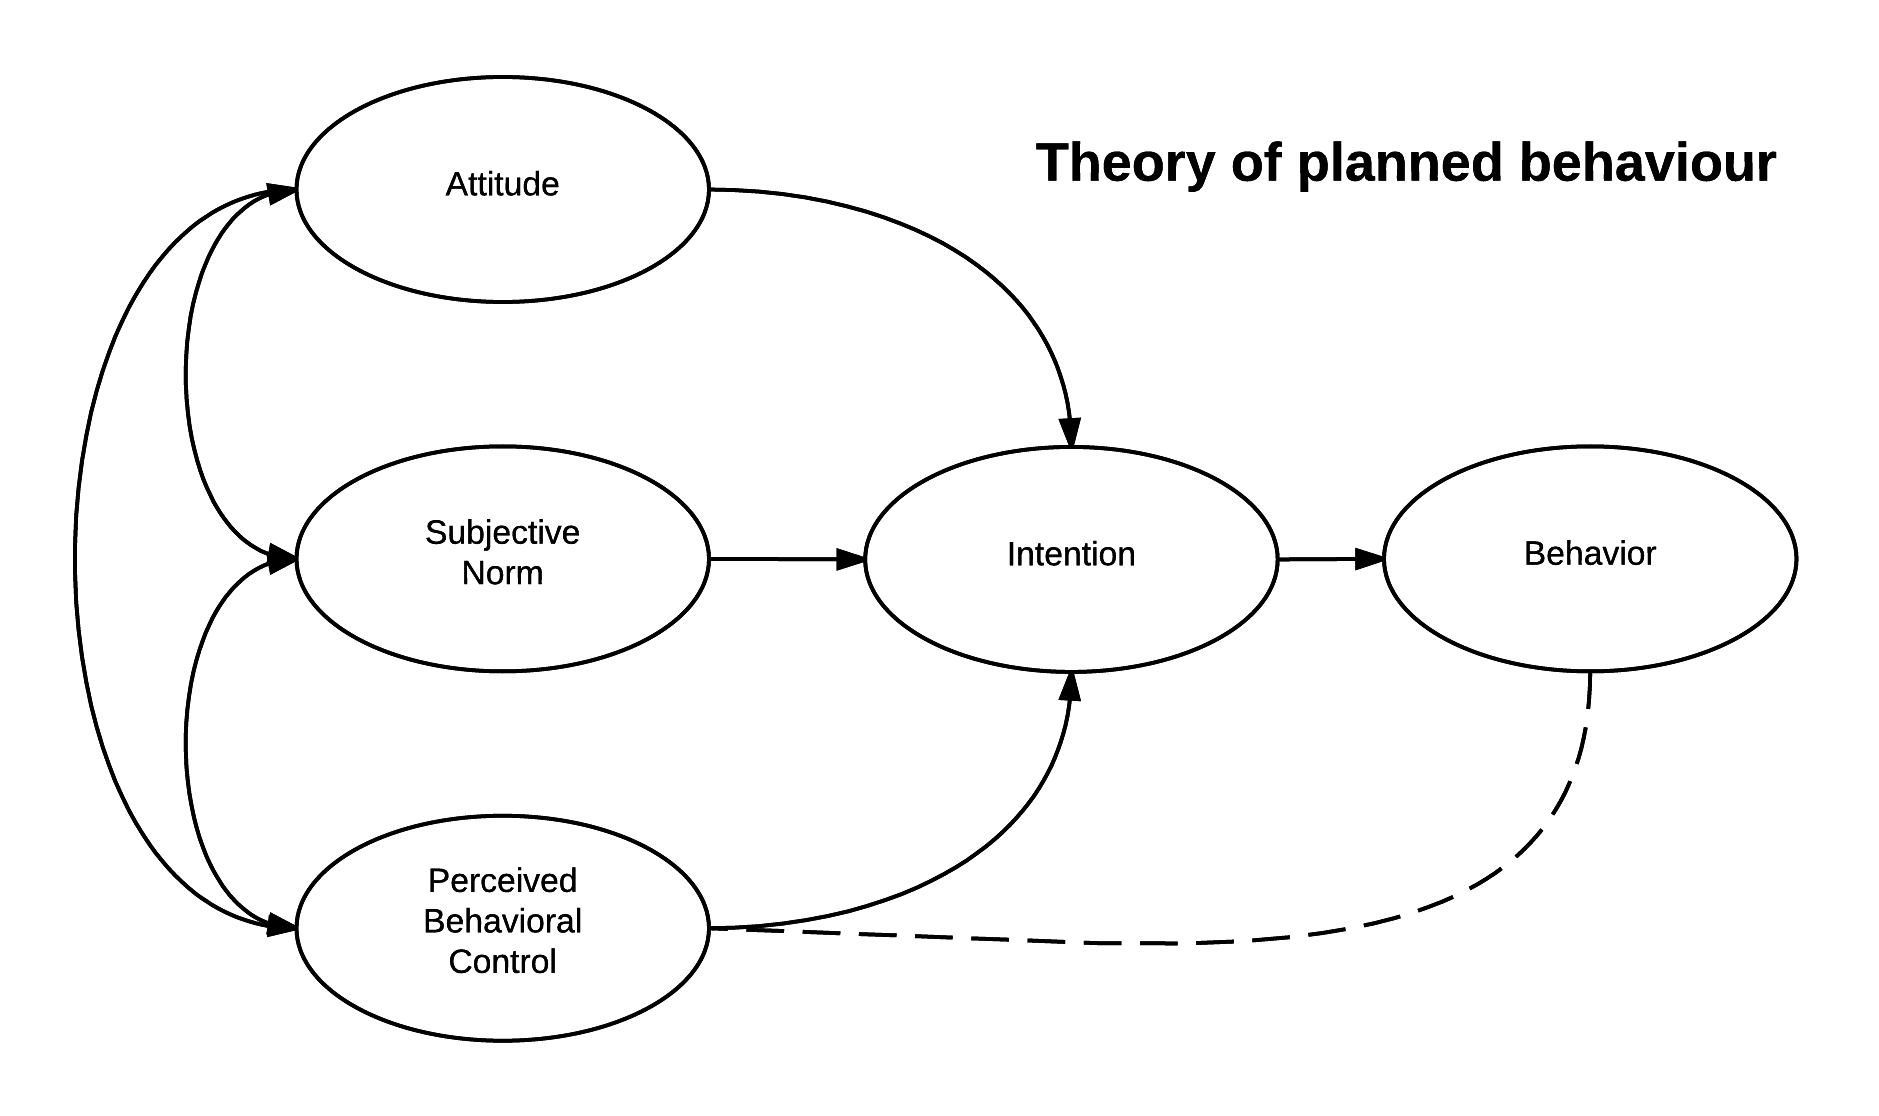
\includegraphics[width=0.8\textwidth]{Theory_of_planned_behavior_chart}}
    \caption{ساختار نظریه رفتار برنامه ریزی شده
      %\cite{kim2016integrated}
    }
    \label{fig:Theory_of_planned_behavior_chart}
  \end{figure}\\

  این نظریه در پژوهش‌های پیشین برای بررسی رفتار
  به اشتراک گذاری داده های خصوصی
  فرد در شبکه اجتماعی فیسبوک استفاده شده است
  \!\cite{vanderschyffInformationPrivacyBehavior2020}
  \!.
  مدلی که
  \!\gls{Theory of planned behavior}
  ارائه پیشنهاد می‌دهد، احتمال وقوع  رفتار‌های ارادی مخصوصا رفتار‌های ارادی مثبت به شدت تمایل فرد به
  انجام آن رفتار بستگی دارد.
  \!({\gls{Icek Ajzen}})
  عامل تعیین کننده برای انجام یک کار تمایلات او است.
\fi
%%%%%%%%%%%%%%%%%%%%

\ifSurveyfillingBehavior
  % بررسی اینکه آیا از نحوه پر کردن فرم ها می توان به کانفیدنس صداقت آزمودنی پی برد یا نه
  در صورتیکه گزینه‌های پرسشنامه اجباری باشند کیفیت داده‌های جمع‌آوری شده کاهش می یابد.
  \!\cite{sischkaImpactForcedAnswering2022}
\fi
% ^ %%%%%%%%%%%%%%%%%%%%%%%%%%%%%%%%%%%%%%%%%%%%%%%%%%%%%%%%%%%%%
% ^ %%%%%%%%%%%%%%%%%%%%%%%%%%%%%%%%%%%%%%%%%%%%%%%%%%%%%%%%%%%%%
% ^ %%%%%%%%%%%%%%%%%%%%%%%%%%%%%%%%%%%%%%%%%%%%%%%%%%%%%%%%%%%%%
\section{اهمیت}
%% توضیح بیشتر اضافه گردد بعدا
پژوهش انجام شده در سال ۲۰۲۰ نشان می دهد که در بازار داده های خصوصی آنلاین بازیگران زیادی به عنوان واسطه وجود دارند.
\!\cite{agogoInvisibleMarketOnline2021}
همچنین با گسترش هر روزه سیستم های اطلاعاتی که به
جمع‌آوری، ذخیره‌سازی، پردازش و به‌اشتراک‌گذاری داده‌های
خصوصی افراد می‌پردازند بررسی فرایندهای
تصمیم گیری و پارامتر‌های تاثیر گذار
بر این تصمیم‌گیری دارای اهمیت شده است
\!.
\!\cite{spiekermannValuesEthicsInformation2022}
از سوی دیگر نگرش افراد تصمیم گیرنده نسبت به ارزش اطلاعات خصوصی افراد می تواند نقش مهمی در رفتار آنها داشته باشد.
پژوهش‌هایی برای اندازه‌گیری ارزش داده‌های خصوصی انجام شده است
\!\cite{  fastValuePersonalData2021a,wesselsSellNotSell2019,tangHowChineseWeb2021}
\ifWillingnessToPay
  مقایسه میان رفتار افراد در پژوهش‌های اندازه‌گیری
  \textit{تمایل به پرداخت}
  \LTRfootnote{willingness to pay}
  نشان داده است که
  \textit{تمایل به پرداخت }
  با استفاده از روش‌های فرضی مانند
  \textit{ارزشيابی مشروط}
  \LTRfootnote{contingent valuation }
  میان ۱۷ تا ۶۳ درصد بالاتر
  از روشهای غیر فرضی مانند
  \textit{حراج تجربی}
  \LTRfootnote{experimental auction}
  است.
  حراج تجربی به عنوان یک روش
  \textit{سازگار با انگیزه}
  \LTRfootnote{incentive compatibility}
  شناسایی شده‌است
  \!\citep{martinez-carrascoComparingHypotheticalNonhypothetical2015}
  .
  یک فرایند،
  \textit{سازگار با انگیزه}
  است وقتی‌که همه شرکت‌کنندگان فقط  با درنظر گرفتن ترجیهات واقعی خود، بهترین خروجی را بدست می‌آورند
  \!\citep{nisanAlgorithmicGameTheory2007}
  \!.


\fi
% ^ %%%%%%%%%%%%%%%%%%%%%%%%%%%%%%%%%%%%%%%%%%%%%%%%%%%%%%%%%%%%%
% ^ %%%%%%%%%%%%%%%%%%%%%%%%%%%%%%%%%%%%%%%%%%%%%%%%%%%%%%%%%%%%%
% ^ %%%%%%%%%%%%%%%%%%%%%%%%%%%%%%%%%%%%%%%%%%%%%%%%%%%%%%%%%%%%%

\section{فرضیه پژوهشی}

% ^ %%%%%%%%%%%%%%%%%%%%%%%%%%%%%%%%%%%%%%%%%%%%%%%%%%%%%%%%%%%%%
% ^ %%%%%%%%%%%%%%%%%%%%%%%%%%%%%%%%%%%%%%%%%%%%%%%%%%%%%%%%%%%%%
% ^ %%%%%%%%%%%%%%%%%%%%%%%%%%%%%%%%%%%%%%%%%%%%%%%%%%%%%%%%%%%%%

% کلیه فایل‌های لازم برای حروف‌چینی با کلاس فوق، داخل پوشه‌ای به نام
% \lr{tehran-thesis}
% قرار داده شده است. توجه داشته باشید که برای استفاده از این کلاس باید فونت‌های
% \lr{IRLotusICEE}
% و
% \lr{IRTitr}
% را داشته باشید (که همراه با این کلاس هست و نیاز به نصب نیست).
% قلم‌های
% \lr{IRLotusICEE}
% مستخرج از قلم‌های استاندارد
% \lr{IRLotus}
% شورای عالی اطلاع‌رسانی%
% \footnote{
% قلم‌های استاندارد
% \lr{IRFonts}
% از شورای عالی اطلاع‌رسانی، منطبق بر آخرین نسخه استاندارد یونیکد، استاندارد ملی ۶۲۱۹ و استاندارد
% \lr{Adobe Glyph Naming}
% هستند.
% }
% هستند که توسط دکتر بابایی‌زاده اصلاحاتی روی آنها صورت پذیرفته است: تبدیل صفر توپر به صفر توخالی (جهت تمایز بیشتر با نقطه) و اضافه شدن
% \textit{\textbf{حالت توپر و ایرانیک توأم}}،
% که این موارد در قلم‌های شورای عالی اطلاع‌رسانی وجود ندارد.

% \subsection{این همه فایل؟!}
% \label{muchFiles}
% از آنجایی که یک پایان‌نامه یا رساله، یک نوشته بلند محسوب می‌شود، لذا اگر همه تنظیمات و مطالب پایان‌نامه را داخل یک فایل قرار بدهیم، باعث شلوغی و سردرگمی می‌شود. به همین خاطر، قسمت‌های مختلف پایان‌نامه یا رساله  داخل فایل‌های جداگانه قرار گرفته است. مثلاً تنظیمات پایه‌ای کلاس داخل فایل
% \lr{tehran-thesis.cls}، 
% قسمت مشخصات فارسی پایان‌نامه داخل 
% \lr{faTitle.tex}،
% مطالب فصل اول داخل 
% \lr{chapter1.tex}
% و تنظیمات قابل تغییر توسط کاربر داخل 
% \lr{commands.tex}،
% قرار داده شده است.
% \textbf{
% 	فایل اصلی این مجموعه، فایل
% 	\lr{main.tex}
% 	می‌باشد.
% }
% % یعنی بعد از تغییر فایل‌های دیگر، برای دیدن نتیجه تغییرات، باید این فایل را اجرا کرد. بقیه فایل‌ها به این فایل، کمک می‌کنند تا بتوانیم خروجی کار را ببینیم.
% اگر به فایل 
% \lr{main.tex}
% دقت کنید، متوجه می‌شوید که قسمت‌های مختلف پایان‌نامه، توسط دستورهایی مانند 
% \lr{input}
% و
% \lr{include}
% به فایل اصلی، یعنی 
% \lr{main.tex}
% معرفی شده‌اند.
% با توجه به ساختار محتوایی دستورالعمل، در فایل
% \lr{main.tex}
% فرض شده که پایان‌نامه یا رساله شما، از ۵ فصل و تعدادی پیوست تشکیل شده است. با اینحال، شما می‌توانید به راحتی فصل‌ها و پیوست‌ها را با صلاحدید اساتید راهنما، کم و زیاد کنید. این کار، بسیار ساده است. فرض کنید بخواهید یک فصل دیگر هم به پایان‌نامه اضافه کنید. برای این کار، کافی است یک فایل با نام دلخواه مثلاً 
% \lr{chapter6}
% و با پسوند 
% \lr{.tex}
% بسازید و آن را داخل پوشه 
% \lr{tehran-thesis}
% قرار دهید و سپس این فایل را با دستور 
% \verb!\include{chapter6}!
% داخل فایل
% \lr{main.tex}
%  فراخوانی کنید.

% \subsection{از کجا شروع کنم؟}
% قبل از هر چیز، باید یک توزیع تِک مناسب مانند تک‌لایو
% \lr{(TeXLive)}
% را روی سیستم خود نصب کنید. تک‌لایو  را می‌توانید از 
%  \href{http://www.tug.org/texlive}{سایت رسمی آن}%
% \LTRfootnote{\lr{\url{http://www.tug.org/texlive}}}
%  دانلود کنید یا مستقیماً از مخازن توزیع لینوکس خود بگیرید (مثلاً در اوبونتو با دستور
% \LRE{\verb!sudo apt install texlive-full!}).
% برای نصب تک‌لایو و اجرای اسناد زی‌پرشین می‌توانید از
% \href{http://parsilatex.com/site/shop/}{دی‌وی‌دی مجموعه پارسی‌لاتک}%
% \LTRfootnote{\lr{\url{http://parsilatex.com/site/shop/}}}
% و فایل راهنمای موجود در آن هم کمک بگیرید.

% برای تایپ و پردازش اسناد لاتک باید از یک ویرایشگر مناسب استفاده کنید. ویرایشگرهای
% \lr{TeXWroks},
% \lr{TeXstudio},
% \lr{Texmaker}
% و
% \lr{BiDiTeXmaker}
% بدین منظور تولید شده‌اند. می‌توان ویرایش‌گر 
%  \href{https://bitbucket.org/srazi/biditexmaker3}{\lr{BiDiTeXmaker}}%
%  \LTRfootnote{\lr{\url{https://bitbucket.org/srazi/biditexmaker3}}}
% را که بویژه برای کار با زی‌پرشین و مطالب دوجهته بهبود یافته است، بهینه‌ترین ویرایشگر لاتک برای کار با اسناد فارسی عنوان کرد.

% حال اگر نوشتن \پ اولین تجربه شما از کار با لاتک است، توصیه می‌شود که یک‌بار به صورت اجمالی، کتاب «%
% \href{http://www.tug.ctan.org/tex-archive/info/lshort/persian/lshort.pdf}{مقدمه‌ای نه چندان کوتاه بر
% \lr{\LaTeXe}}%
% \LTRfootnote{\lr{\url{http://www.tug.ctan.org/tex-archive/info/lshort/persian/lshort.pdf}\hfill}}»
% ترجمه دکتر مهدی امیدعلی را مطالعه کنید. این کتاب، کتاب بسیار کاملی است که خیلی از نیازهای شما در ارتباط با حروف‌چینی را برطرف می‌کند.
% اگر تک لایو کامل را داشته باشید، این کتاب را هم دارید. کافیست در خط فرمان دستور زیر را بزنید:
% \begin{latin}
% 	\texttt{texdoc lshort-persian}
% \end{latin}
% اگر عجله دارید، برخی دستورات پایه‌ای مورد نیاز در پیوست \ref{app:latexIntro} بیان شده‌اند.

% بعد از موارد گفته شده، فایل 
% \lr{main.tex}
% و
% \lr{faTitle.tex}
% را باز کنید و مشخصات پایان‌نامه خود مثل نام، نام خانوادگی، عنوان پایان‌نامه و ... را جایگزین مشخصات موجود در فایل
% \lr{faTitle.tex}
%  کنید. نیازی نیست نگران چینش این مشخصات در فایل پی‌دی‌اف خروجی باشید، زیرا کلاس 
% \lr{tehran-thesis}
% همه این کارها را بطور خودکار برای شما انجام می‌دهد. در ضمن، موقع تغییر دادن دستورهای داخل فایل
% \lr{faTitle.tex}
%  کاملاً دقت کنید؛ این دستورها، خیلی حساس هستند و ممکن است با یک تغییر کوچک، موقع اجرا، خطا بگیرید. برای دیدن خروجی کار، فایل 
% \lr{faTitle.tex}
%  را 
% \lr{Save}
% (نه 
% \lr{Save As})
% کنید و بعد به فایل 
% \lr{main.tex}
% برگشته و آن را اجرا کنید%
% \footnote{
% 	البته فایلهای این مجموعه به گونه‌ای هستند که در
% 	\lr{TeXWorks} یا
% 	\lr{TeXstudio}
% 	بدون بازگشت به فایل اصلی، می‌توانید سند خود را اجرا کنید.
% }.
%  حال اگر می‌خواهید مشخصات انگلیسی \پ را هم عوض کنید، فایل 
% \lr{enTitle.tex}
% را باز کنید و مشخصات داخلش را تغییر دهید.
% %\RTLfootnote{
% %برای نوشتن پروژه کارشناسی، نیازی به وارد کردن مشخصات انگلیسی پروژه نیست. بنابراین، این مشخصات بطور خودکار، نادیده گرفته می‌شود.
% %}
% در اینجا هم برای دیدن خروجی باید این فایل را ذخیره کرده، بعد به فایل 
% \lr{main.tex}
% برگشته و آن را اجرا کرد.

% برای راحتی بیشتر، کلاس 
% \lr{tehran-thesis.cls}
% طوری طراحی شده است که کافی است فقط  یک‌بار مشخصات \پ را (در فایل‌های
% \lr{faTitle.tex}
% و
% \lr{enTitle.tex})
% وارد کنید و هر جای دیگر که این مشخصات لازم باشند، به طور خودکار درج می‌شوند. با این حال، اگر مایل بودید، می‌توانید تنظیمات موجود را تغییر دهید؛ گرچه، در صورتیکه کاربر مبتدی هستید و یا با ساختار فایل‌های  
% \lr{cls}
%  آشنایی ندارید، بهتر است به فایل 
% \lr{tehran-thesis.cls}
% دست نزنید.

% نکته دیگری که باید به آن توجه کنید این است که در قالب آماده شده، سه گزینه به نام‌های
% \lr{bsc}،
% \lr{msc}
% و
% \lr{phd}
% برای نوشتن پروژه، پایان‌نامه و رساله، در نظر گرفته شده است. بنابراین اگر قصد تایپ پروژهٔ کارشناسی، پایان‌نامهٔ کارشناسی ارشد یا رسالهٔ دکتری را دارید، به ترتیب باید از گزینه‌های
% \lr{bsc}،
% \lr{msc}
% و
% \lr{phd}
% در فایل 
% \lr{main.tex}
% استفاده کنید. با انتخاب هر کدام از این گزینه‌ها، تنظیمات مربوط به آنها به طور خودکار، اعمال می‌شود.


% \subsection[مطالب پایان‌نامه را چطور بنویسم؟]
% {مطالب \پ را چطور بنویسم؟}
% \subsubsection{نوشتن فصل‌ها}
% همان‌طور که در بخش \ref{muchFiles} گفته شد برای جلوگیری از شلوغی، قسمت‌های مختلف \پ از جمله فصل‌ها، در فایل‌های جداگانه‌ای قرار داده شده‌اند. 
% مثلاً اگر می‌خواهید مطالب فصل ۱ را تایپ کنید، باید فایل‌های 
% \lr{main.tex}
% و
% \lr{chapter1.tex}
% را باز کرده و مطالب خود را جایگزین محتویات داخل 
% \lr{chapter1.tex}
% نمایید. دقت شود که در ابتدای برخی فایلها دستوراتی نوشته شده است و از شما خواسته شده که آن دستورات را حذف نکنید.

%توجه کنید که همان‌طور که قبلاً هم گفته شد، تنها فایل قابل اجرا، 
%\lr{main.tex}
%است. لذا برای دیدن حاصل (خروجی) فایل خود، باید  
%\lr{chapter1.tex}
%را ذخیره کرده و سپس فایل 
%\lr{main.tex}
%را اجرا کنید.

% نکته بسیار مهمی که در اینجا باید گفته شود این است که سیستم \lr{\TeX}، محتویات یک فایل تِک را به ترتیب پردازش می‌کند.  بنابراین، اگر مثلاً  دو فصل اول خود را نوشته و خروجی آنها را دیده‌اید و مشغول تایپ مطالب فصل ۳ هستید، بهتر است
% که دو دستور 
% \verb!\include{chapter1}!
% و
% \verb!\include{chapter2}!
% را در فایل 
% \lr{main.tex}،
% غیرفعال%
% \footnote{
% برای غیرفعال کردن یک دستور، کافی است در ابتدای آن، علامت درصد انگلیسی (\%) بگذارید.
% }
%  کنید. در غیر این صورت، ابتدا مطالب دو فصل اول پردازش شده و سپس مطالب فصل ۳ پردازش می‌شود که این کار باعث طولانی شدن زمان پردازش می‌گردد. هر زمان که خروجی کل \پ را خواستید، تمام فصل‌ها را دوباره در
% \lr{main.tex}
% فعال نمائید.
% بدیهتاً لازم نیست فصل‌های \پ را به ترتیب تایپ کنید. مثلاً می‌توانید ابتدا مطالب فصل ۳ را تایپ نموده و سپس مطالب فصل ۱ را تایپ کنید. 
% \subsubsection{مراجع}
% برای وارد کردن مراجع \پ کافی است فایل 
% \lr{MyReferences.bib}
% را باز کرده و مراجع خود را به شکل اقلام نمونهٔ داخل آن، وارد کنید.  سپس از \lr{bibtex} برای تولید مراجع با قالب مناسب استفاده نمائید. برای توضیحات بیشتر بخش \ref{Sec:Ref} از پیوست \ref{app:latexIntro} و نیز پیوست \ref{app:refMan} را ببینید.

% \subsubsection{واژه‌نامه فارسی به انگلیسی و برعکس}
% برای وارد کردن معادل فارسی اصطلاحات لاتین در متن و تهیه فهرست واژه‌نامه از آنها، از بستهٔ
% \lr{glossaries}
% و نرم‌افزار
% \lr{xindy}
% استفاده می‌شود. بدین منظور کافی است اصطلاحات لاتین و ترجمهٔ آنها را در فایل
% \lr{words.tex}
% وارد کرده و هر جای متن که خواستید با دستورات
% \verb|gls{label}|
% یا \verb|glspl{label}|
% معادل فارسی مفرد یا جمع یک اصطلاح را بیاورید.

% مثلا در اینجا، واژهٔ
% «\gls{Action}»
% برای بار اول و دوباره
% «\gls{Action}»
% برای بار دوم در متن ظاهر شده است.
% جهت توضیحات بیشتر به پیوست
% \ref{app:refMan}
% مراجعه کنید.
% \subsubsection{نمایه}
% برای وارد کردن نمایه، باید از 
% \lr{xindy}
% استفاده کنید. 
%زیرا 
%\lr{MakeIndex}
%با حروف «گ»، «چ»، «پ»، «ژ» و «ک» مشکل دارد و ترتیب الفبایی این حروف را رعایت نمی‌کند. همچنین، فاصله بین هر گروه از کلمات در 
%\lr{MakeIndex}،
%به درستی رعایت نمی‌شود که باعث زشت شدن حروف‌چینی این قسمت می‌شود. 
% راهنمای چگونگی کار با 
% \lr{xindy} 
% را می‌توانید در ویکی پارسی‌لاتک و یا مثالهای موجود در دی‌وی‌دی «مجموعه پارسی‌لاتک»، پیدا کنید.

% \subsection{اگر سوالی داشتم، از کی بپرسم؟}
% برای پرسیدن سوال‌های خود موقع حروف‌چینی با زی‌پرشین، می‌توانید به
% \href{http://qa.parsilatex.com}{سایت پرسش و پاسخ پارسی‌لاتک}%
% \LTRfootnote{http://qa.parsilatex.com}
% یا
% \href{http://forum.parsilatex.com}{بایگانی تالارگفتگوی قدیمی پارسی‌لاتک}%
% \mypagestye{http://forum.parsilatex.com}
% مراجعه کنید. شما هم می‌توانید روزی به سوال‌های دیگران در اینترنت جواب دهید.
% بستهٔ زی‌پرشین و بسیاری از بسته‌های مرتبط با آن مانند
% \lr{bidi} و
% \lr{Persian-bib}،
% مجموعه پارسی‌لاتک، مثالهای مختلف موجود در آن، قالب پایان‌نامه دانشگاههای مختلف و سایت پارسی‌لاتک همه به صورت داوطلبانه توسط افراد گروه پارسی‌لاتک و گروه
% \lr{Persian TeX}
% و بدون هیچ کمک مالی انجام شده‌اند. کار اصلی نوشتن و توسعه زی‌پرشین توسط آقای وفا خلیقی انجام شده است که این کار بزرگ را به انجام رساندند.
% اگر مایل به کمک به گروه پارسی‌لاتک هستید به سایت این گروه مراجعه فرمایید:
% \begin{center}
% 	\url{http://www.parsilatex.com}
% \end{center}

% \section{محتویات فصل اول یک پایان‌نامه}
% فصل اول یک پایان‌نامه باید به مقدمه یا کلیات تحقیق بپردازد.
% هدف از فصل مقدمه%
% \LTRfootnote{Introduction}،
% شرح مختصر مسأله تحقیق، اهمیت و انگیزه محقق از پرداختن به آن موضوع، بهمراه اشاره‌ای كوتاه به روش و مراحل تحقیق است. مقدمه، اولين فصل از ساختار اصلی \پ بوده و زمینه اطلاعاتی لازم را برای خواننده فراهم می‌آورد. در طول مقدمه باید سعی شود موضوع تحقیق با زبانی روشن، ساده و بطور عمیق و هدفمند به خواننده معرفی شود. این فصل باید خواننده را مجذوب و اهميت موضوع تحقيق را آشکار سازد. در مقدمه باید با ارائهٔ سوابق، شواهد تحقيقی و اطلاعات موجود (با ذکر منبع) با روشی منظم، منطقی و هدف‌دار، خواننده را جهت داد و به سوی راه حل مورد نظر هدايت کرد. مقدمه مناسب‌ترين جا برای ارائهٔ اختصارات و بعضی توضيحات کلی است، توضيحاتی که شايد نتوان در مباحث ديگر آنها را شرح داد.

% مقدمه، یکی از ارکان اساسی و اصلی پایان نامه است که مهمترین قسمت‌های آن عبارتند از: 

% \subsection{عنوان تحقیق} 
% باید شناختی دقیق و روشن از حوزهٔ موضوع تحقیق را عرضه دارد و خالی از هرگونه ابهام و پیچیدگی باشد.

% \subsection{مسأله تحقیق}
% وظیفه اصلی مقدمه بیان این مطلب به خواننده است که چرا انجام تحقیق را به عهده گرفته‌اید. اگر دلیل شما برای انجام این کار پاسخگویی به سؤال مورد علاقه‌تان است، با مشکل زیادی روبه‌رو نخواهید بود. یکی از بهترین روش‌ها برای نوشتن مقدمهٔ یک پایان‌نامه، طرح پرسش یا پرسش‌هایی مهم و اساسی است که کار تحقیقاتی شما از آغاز تا پایان قصد پاسخ دادن به آن را دارد. گاهی می‌توانید ابتدا اهمیت موضوع را بیان و سپس پرسش خود را در آن موضوع مطرح کنید.

% \subsection{تاریخچه‌ای از موضوع تحقیق}
% به طور کلی تشریح روندهای تحقیقاتی در محدودهٔ مورد مطالعه، مستلزم ارجاع به کارهای دیگران است. بعضی از نویسندگان برای کارهای دیگران هیچ اعتباری قائل نمی‌شوند و در مقابل، بعضی دیگر از نویسندگان در توصیف کارهای دیگران، بسیار زیاده‌روی می‌کنند. اکثر مواقع، ارجاع به مقالات دو سال قبل از کارتان، بهتر از نوشتن سطرهای مرجع است. در این قسمت باید به طور مختصر به نظرات و تحقیقات مربوط به موضوع و یا مسائل و مشکلات حل نشده در این حوزه و همچنین توجه و علاقه جامعه به این موضوع، اشاره شود.

% \subsection{تعریف موضوع تحقیق}
% در این قسمت محقق، موضوع مورد علاقه و یا نیاز احساس شدهٔ خود را در حوزه تحقیق بیان می‌دارد و عوامل موجود در موقعیت را تعریف و تعیین می‌کند.

% \subsection{هدف یا هدف‌های کلی و آرمانی تحقیق}
% این قسمت باید با جملات مثبت و کلی طرح شود و از طولانی شدن مطالب پرهیز شود.

% \subsection{روش انجام تحقیق}
% در این قسمت، پژوهشگر روش کاری خود را بیان می‌دارد و شیوه‌های گوناگونی را که در گردآوری مطالب خود بکار برده، ذکر می‌کند. همچنین اگر روش آماری خاصی را در تهیه و تدوین اطلاعات به کار برده است، آن شیوه را نیز اینجا بیان می‌کند.

% \subsection{نوآوری، اهمیت و ارزش تحقیق}
% در این قسمت، در مورد نوآوری علمی و عملی تحقیق که محقق به آن دست خواهد یافت، بحث می‌شود. ممکن است لازم باشد تا برخی نمودارهای خلاصه در این بخش استفاده شوند. به عنوان مثال، نموداری از مقاله
% \cite{kim2016integrated}
% در شکل
% \ref{fig:sampleDiagram}
% آمده است.
% \begin{figure}[ht]
% 	\centerline{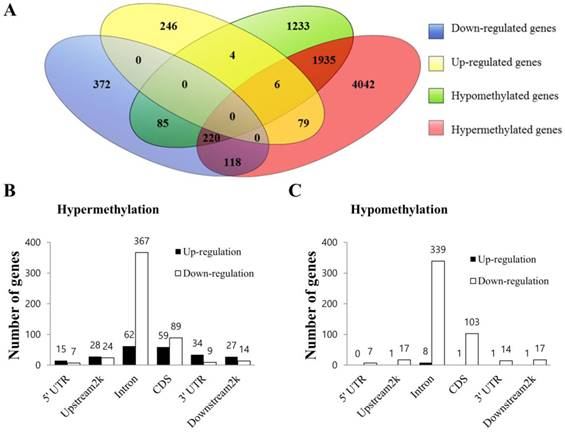
\includegraphics[width=0.8\textwidth]{journal-of-cancer_sample-result}}
% 	\caption{یک نمونه نمودار خلاصه برای نمایش نوآوری در نتایج
% 		%\cite{kim2016integrated}
% 	}
% 	\label{fig:sampleDiagram}
% \end{figure}\\
% طبیعتاً به صلاحدید نگارنده، شکل‌ها و نمودار‌ها می توانند در بخش های مختلف، خصوصا فصل
% \ref{chap:results}
% مورد استفاده قرار گیرند.

\subsection{تعریف واژه‌ها (اختیاری)}
% در این قسمت محقق باید واژه‌هایی را که ممکن است برای خواننده آشنا نباشد، تعریف کند.

\subsection{خلاصه فصل‌ها}
% در آخرین قسمتِ فصل اول پایان‌نامه، خلاصه‌ای اشاره‌وار از فصل‌های آتی آورده می‌شود تا خواننده بتواند تصویری واضح از دیگر قسمت‌های پایان‌نامه در ذهن خود ترسیم کند.

\section{جمع‌بندی}
% در این فصل به دو مقولهٔ نحوه استفاده از قالب \پ دانشگاه تهران و نیز ویژگی‌هایی که محتویات فصل اول پایان‌نامه (یعنی مقدمه) باید داشته باشند، پرداخته شد. با توجه به اینکه این راهنما نحوه استفاده از قالب را شرح داده، ملزومات محتوایی هر فصل پایان‌نامه را توضیح می‌دهد و در پیوست‌ها نیز نحوهٔ کار با لاتک را یادآوری خواهد کرد، بنابراین مطالعهٔ کامل آن مقداری وقت شما را خواهد گرفت؛ اما مطمئن باشید از اتلاف وقت شما در ادامه کارتان تا حد زیادی جلوگیری خواهد کرد. در نوشتن متن حاضر سعی شده است علاوه بر ایجاد یک قالب لاتک برای پایان‌نامه‌های دانشگاه تهران، نکات محتوایی هر فصل نیز گوشزد گردد. طبیعتاً برای نگارش پایان‌نامهٔ خود می‌بایست مطالب تمام فصل‌ها را خودتان بازنویسی کنید.

% در ادامهٔ این راهنما، تنها فصل‌هایی که یک پایان‌نامه باید داشته باشد و نیز خصوصیات یا ساختاری که محتویات هر فصل باید از آنها برخوردار باشد%
% \footnote{از روی فایل «تمپلیت نگارش و تدوین پایان‌نامه \cite{UTThesisGuide}»}،
% آورده می‌شوند. نهایتاً  در پیوست‌ها، مطالبی در باب یادآوری دستورات لاتک، نحوه نوشتن فرمول‌ها، تعاریف، قضایا، مثال‌ها، درج تصاویر، نمودارها، جداول و الگوریتم‌ها و نیز مدیریت مراجع، آمده است.

% همچنین توصیه اکید دارم که رفع خطاهایی که احتمالاً با آنها مواجه می‌شوید را به آخر موکول نفرمایید و به محض برخورد با خطا، آن را اشکال‌زدایی و برطرف نمائید.!
% و
% \verb!% !TeX root=main.tex
\chapter{مروری بر مطالعات انجام شده}
%\thispagestyle{empty} 
\section{مقدمه}
% هدف از اين فصل که با عنوان‌های  «مروری بر ادبیات موضوع%
% \LTRfootnote{Literature Review}»،
% «مروری بر منابع» و يا «مروری بر پیشینه تحقیق%
% \LTRfootnote{Background Research}»
% معرفی می‌شود، بررسی و طبقه‌بندی یافته‌های تحقیقات دیگر محققان در سطح دنیا و تعیین و شناسایی خلأهای تحقیقاتی است. آنچه را که تحقیق شما به دانش موجود اضافه می‌کند، مشخص کنید. طرح پیشینه تحقیق%
% \LTRfootnote{Background Information}
% یک مرور محققانه است و تا آنجا باید پیش برود که پیش‌زمینهٔ تاریخی مناسبی از تحقیق را بیان کند و جایگاه تحقیق فعلی را در میان آثار پیشین نشان دهد. برای این منظور منابع مرتبط با تحقیق را بررسی کنید، البته نه آنچنان گسترده که کل پیشینه تاریخی بحث را در برگیرد. برای نوشتن این بخش:
% \begin{itemize}
% 	\item
% 	دانستنی‌های موجود و پیش‌زمینهٔ تاریخی و وضعیت کنونی موضوع را چنان بیان کنید که خواننده بدون مراجعه به منابع پیشین، نتایج حاصل از مطالعات قبلی را درک و ارزیابی کند.
% 	\item
% 	نشان دهید که بر موضوع احاطه دارید. پرسش تحقیق را همراه بحث و جدل‌ها و مسائل مطرح شده بیان کنید و مهم‌ترین تحقیق‌های انجام شده در این زمینه را معرفی نمائید.
% 	\item
% 	ابتدا مطالب عمومی‌تر و سپس پژوهش‌های مشابه با کار خود را معرفی کرده و نشان دهید که تحقیق شما از چه جنبه‌ای با کار دیگران تشابه یا تفاوت دارد.
% 	\item
% 	اگر کارهای قبلی را خلاصه کرده‌اید، از پرداختن به جزئیات غیرضروری بپرهیزید. در عوض، بر یافته‌ها و مسائل روش‌شناختی مرتبط و نتایج اصلی تأکید کنید و اگر بررسی‌ها و منابع مروری عمومی دربارهٔ موضوع موجود است، خواننده را به آنها ارجاع دهید.
% \end{itemize}


% \section{مروری بر ادبیات موضوع}
% در این قسمت باید به کارهای مشابه دیگران در گذشته اشاره کرد و وزن بیشتر این قسمت بهتر است به مقالات ژورنالی سال‌های اخیر (۲ تا ۳ سال) تخصیص داده شود. به نتایج کارهای دیگران با ذکر دقیق مراجع باید اشاره شده و جایگاه و تفاوت تحقیق شما نیز با کارهای دیگران مشخص شود. استفاده از مقالات ژورنال‌های معتبر در دو یا سه سال اخیر، می‌تواند به اعتبار کار شما بیافزاید.

% \section{نتیجه‌گیری}
% ‌در نتیجه‌گیری آخر این فصل، با توجه به بررسی انجام شده بر روی مراجع تحقيق، بخش‌های قابل گسترش و تحقیق در آن حیطه و چشم‌اندازهای تحقیق مورد بررسی قرار می‌گیرند.	در برخی از تحقیقات، نتیجه نهایی فصل روش تحقیق، ارائهٔ یک چارچوب کار تحقیقی 
% \lr{(research framework)}
% است.
\ifExperimentalAuction
	تصمیم‌گیری های ما نمایشگر ارزشگذاری‌های ما هستند. اقتصاد‌دان‌ها
	\textit{ارزش اقتصادی}
	\LTRfootnote{economic value}
	این تصمیمات را با نرخی که فرد یک محصول یا دارایی را با  دیگری مبادله می کند ، بیان می‌کنند.
	این نرخ به وسیله
	\textit{تمایل به پرداخت }
	\LTRfootnote{willingness to pay}
	حداکثری فرد اندازه‌گیری می‌شود.
	\citep{luskExperimentalAuctionsMethods2007}
	\section{تعاریف، اصول و مبانی نظری}
	% این قسمت ارائهٔ خلاصه‌ای از دانش کلاسیک موضوع است. این بخش الزامی نیست و بستگی به نظر استاد راهنما دارد.

\fi

\ifTheEffectsOfDifferentPersonalData
	\textit{چاو، اوی و هربلاند}
	\LTRfootnote{Chua, H.N., J.S. Ooi, and A. Herbland}
	در سال ۲۰۲۱ اطلاعات شخصی را در ۶ دسته طبقه بندی کرده‌اند.
	\citep{chuaEffectsDifferentPersonal2021}
	جدول
	\eqref{tab:PICatAndChar}
	\begin{table}[ht]
		\caption{دسته‌ها و ویژگی‌های اطلاعت شخصی}
		\label{tab:PICatAndChar}
		\centering
		\onehalfspacing
		% \begin{tabular}{p{0.35\linewidth} | p{0.6\linewidth}}  
		\begin{tabularx}{\linewidth}{ r X }
			% \hline 
			دسته
			 &
			% درجه آزادی 
			% تبدیل مختصات &
			توضیح
			\\
			\hline
			سبک زندگی-رفتار(LB)
			 &
			% zotero://select/library/items/LCYS3GQ2
			% https://www.zotero.org/users/5038267/items/LCYS3GQ2
			%توضیح
			اطلاعت درباره ویژگی‌ها و سبک زندگی فرد که بر رابطه عاطفی یا
			اجتماعی، ترجیهات، عادات، باورها، یا دیدگاه‌های او اثر می‌گذارد.
			% مثال‌ها:
			% \lr{L1}:
			% باور
			% (
			% مانند باورهای مذهبی، باورهای فلسفی، افکار و غیره
			% )
			% % \hline 
			% \lr{L2}:
			% ترجیهات و علایق
			% (مانند نظرات، تمایلات، علایق، غذاهای مورد علاقه، رنگ‌ها، چیزهای
			% دوست‌داشتنی و دوست‌نداشتنی)
			% \lr{L3}:
			% رفتار
			% (مانند رفتار وبگردی، الگوی تماس‌ها، لینک‌های کلیک شده،
			% سبک زندگی رویکرد و غیره)
			% \lr{L4}:
			% خانواده/روابط عاطفی
			% (مانند ساختار خانواده، همشیرها، فرزندان، ازدواج‌ها، طلاق‌ها،
			% روابط عاطفی و غیره)
			\\
			اجتماعی-اقتصادی(SE)
			 &
			% ۳ & 
			% ویژگی دو &
			اطلاعاتی که سطح زندگی اقتصادی یا اجتماعی فرد را نشان می‌دهند یا
			می‌توان به وسیله این اطلاعات ویژگی‌های مزبور را استخراج کرد.
			% مثال‌ها;
			% \lr{S1}:
			% \lr{S1}:
			% \lr{S1}:
			\\
			ردیابی(T)
			 &
			اطلاعاتی که روش‌هایی را برای موقعیت‌یابی و تماس با فرد ایجاد می کند.
			% \hline 
			\\
			اقتصادی(F)
			 &
			اطلاعاتی که درآمد، حساب‌های مالی، اعتبار، توانایی خرید/خرج کردن، و
			دارایی‌های مورد تملک/اجاره شده/قرض گرفته شده را مشخص می کند.
			\\
			احراز هویت(A)
			 &
			اطلاعاتی که برای احراز هویت فرد به کار می‌روند.
			\\
			پزشکی-سلامت(MH)
			 &
			شرایط پزشکی  یا اطلاعات مرتبط با سلامت فرد.
			\\
		\end{tabularx}
	\end{table}
	% \begin{table}[ht]
	%     \caption{مدلهای تبدیل دیگر.}
	%     \label{tab:motionModelsCont}
	%     \centering
	%     \onehalfspacing
	%     \begin{tabularx}{\textwidth}{|r|c|l|X|}
	%         \hline نام مدل & درجه آزادی & تبدیل مختصات & توضیح \\ 
	%         \hline مشابهت & ۴ & $\begin{aligned} x'=sx\cos\theta - sy\sin\theta+t_x \\ y'=sx\sin\theta+sy\cos\theta+t_y  \end{aligned}$  & اقلیدسی+تغییرمقیاس \\ 		
	%         \hline آفین & ۶ & $\begin{aligned} x'=a_{11}x+a_{12}y+t_x \\ y'=a_{21}x+a_{22}y+t_y \end{aligned}$  & مشابهت+اریب‌شدگی \\
	%         \hline
	%     \end{tabularx}
	% \end{table}


	از سوی دیگر
\fi %TheEffectsOfDifferentPersonalData
\ifMultidimensionalNatureOfPrivacyRisksConceptualisationMeasurementAndImplicationsForDigitalServices
	در سال ۲۰۲۲
	\textit{
		\gls{Sabrina Karwatzki, Manuel Trenz and Daniel Veit}
	}
	 یک دسته‌بندی قاعده‌گرا
	\textit{
		\gls{Nomological}
	}
	و جامع از نگرانی‌های حریم خصوصی افراد بر اساس پژوهش های گذشته ارائه داده و اعتبار و روایی آن‌را مورد سنجش قرار‌داده‌اند
	\citep{karwatzkiMultidimensionalNaturePrivacy}
	\!.
	آنها ۷ دسته
	\textbf{
		خطر حریم خصوصی فیزیکی
		\lr{(PH)}
		\LTRfootnote{Physical privacy risk}
		،
		خطر حریم خصوصی اجتماعی
		\lr{(SO)}
		\LTRfootnote{Social privacy risk}
		،
		خطر حریم خصوصی مرتبط با منابع
		\lr{(RE)}
		\LTRfootnote{Resource-related privacy risk}
		،
		خطر حریم خصوصی روانشناختی
		\lr{(PS)}
		\LTRfootnote{Psychological privacy risk}
		،
		خطر حریم خصوصی مرتبط با تعقیب قانونی
		\lr{(PR)}
		\LTRfootnote{Prosecution-related privacy risk}
		،
		خطر حریم خصوصی مرتبط با شغل
		\lr{(CR)}
		\LTRfootnote{Career-related privacy risks}
		\textmd{و}
		خطر حریم خصوصی مرتبط با آزادی
		\lr{(FR)}
		\LTRfootnote{Freedom-related privacy risk}
	}
\fi %\ifMultidimensionalNatureOfPrivacyRisksConceptualisationMeasurementAndImplicationsForDigitalServices
را شناسایی کردند. ما
از این دسته‌بندی و توصیفاتی که در این پژوهش با دسته‌بندی‌های نامبرده مرتبط دانسته شده اند، استفاده کردیم.
!
% را در فایل 
% \lr{main.tex}،
% غیرفعال%
% \footnote{
% برای غیرفعال کردن یک دستور، کافی است در ابتدای آن، علامت درصد انگلیسی (\%) بگذارید.
% }
%  کنید. در غیر این صورت، ابتدا مطالب دو فصل اول پردازش شده و سپس مطالب فصل ۳ پردازش می‌شود که این کار باعث طولانی شدن زمان پردازش می‌گردد. هر زمان که خروجی کل \پ را خواستید، تمام فصل‌ها را دوباره در
% \lr{main.tex}
% فعال نمائید.
% بدیهتاً لازم نیست فصل‌های \پ را به ترتیب تایپ کنید. مثلاً می‌توانید ابتدا مطالب فصل ۳ را تایپ نموده و سپس مطالب فصل ۱ را تایپ کنید. 
% \subsubsection{مراجع}
% برای وارد کردن مراجع \پ کافی است فایل 
% \lr{MyReferences.bib}
% را باز کرده و مراجع خود را به شکل اقلام نمونهٔ داخل آن، وارد کنید.  سپس از \lr{bibtex} برای تولید مراجع با قالب مناسب استفاده نمائید. برای توضیحات بیشتر بخش \ref{Sec:Ref} از پیوست \ref{app:latexIntro} و نیز پیوست \ref{app:refMan} را ببینید.

% \subsubsection{واژه‌نامه فارسی به انگلیسی و برعکس}
% برای وارد کردن معادل فارسی اصطلاحات لاتین در متن و تهیه فهرست واژه‌نامه از آنها، از بستهٔ
% \lr{glossaries}
% و نرم‌افزار
% \lr{xindy}
% استفاده می‌شود. بدین منظور کافی است اصطلاحات لاتین و ترجمهٔ آنها را در فایل
% \lr{words.tex}
% وارد کرده و هر جای متن که خواستید با دستورات
% \verb|gls{label}|
% یا \verb|glspl{label}|
% معادل فارسی مفرد یا جمع یک اصطلاح را بیاورید.

% مثلا در اینجا، واژهٔ
% «\gls{Action}»
% برای بار اول و دوباره
% «\gls{Action}»
% برای بار دوم در متن ظاهر شده است.
% جهت توضیحات بیشتر به پیوست
% \ref{app:refMan}
% مراجعه کنید.
% \subsubsection{نمایه}
% برای وارد کردن نمایه، باید از 
% \lr{xindy}
% استفاده کنید. 
%زیرا 
%\lr{MakeIndex}
%با حروف «گ»، «چ»، «پ»، «ژ» و «ک» مشکل دارد و ترتیب الفبایی این حروف را رعایت نمی‌کند. همچنین، فاصله بین هر گروه از کلمات در 
%\lr{MakeIndex}،
%به درستی رعایت نمی‌شود که باعث زشت شدن حروف‌چینی این قسمت می‌شود. 
% راهنمای چگونگی کار با 
% \lr{xindy} 
% را می‌توانید در ویکی پارسی‌لاتک و یا مثالهای موجود در دی‌وی‌دی «مجموعه پارسی‌لاتک»، پیدا کنید.

% \subsection{اگر سوالی داشتم، از کی بپرسم؟}
% برای پرسیدن سوال‌های خود موقع حروف‌چینی با زی‌پرشین، می‌توانید به
% \href{http://qa.parsilatex.com}{سایت پرسش و پاسخ پارسی‌لاتک}%
% \LTRfootnote{http://qa.parsilatex.com}
% یا
% \href{http://forum.parsilatex.com}{بایگانی تالارگفتگوی قدیمی پارسی‌لاتک}%
% \mypagestye{http://forum.parsilatex.com}
% مراجعه کنید. شما هم می‌توانید روزی به سوال‌های دیگران در اینترنت جواب دهید.
% بستهٔ زی‌پرشین و بسیاری از بسته‌های مرتبط با آن مانند
% \lr{bidi} و
% \lr{Persian-bib}،
% مجموعه پارسی‌لاتک، مثالهای مختلف موجود در آن، قالب پایان‌نامه دانشگاههای مختلف و سایت پارسی‌لاتک همه به صورت داوطلبانه توسط افراد گروه پارسی‌لاتک و گروه
% \lr{Persian TeX}
% و بدون هیچ کمک مالی انجام شده‌اند. کار اصلی نوشتن و توسعه زی‌پرشین توسط آقای وفا خلیقی انجام شده است که این کار بزرگ را به انجام رساندند.
% اگر مایل به کمک به گروه پارسی‌لاتک هستید به سایت این گروه مراجعه فرمایید:
% \begin{center}
% 	\url{http://www.parsilatex.com}
% \end{center}

% \section{محتویات فصل اول یک پایان‌نامه}
% فصل اول یک پایان‌نامه باید به مقدمه یا کلیات تحقیق بپردازد.
% هدف از فصل مقدمه%
% \LTRfootnote{Introduction}،
% شرح مختصر مسأله تحقیق، اهمیت و انگیزه محقق از پرداختن به آن موضوع، بهمراه اشاره‌ای كوتاه به روش و مراحل تحقیق است. مقدمه، اولين فصل از ساختار اصلی \پ بوده و زمینه اطلاعاتی لازم را برای خواننده فراهم می‌آورد. در طول مقدمه باید سعی شود موضوع تحقیق با زبانی روشن، ساده و بطور عمیق و هدفمند به خواننده معرفی شود. این فصل باید خواننده را مجذوب و اهميت موضوع تحقيق را آشکار سازد. در مقدمه باید با ارائهٔ سوابق، شواهد تحقيقی و اطلاعات موجود (با ذکر منبع) با روشی منظم، منطقی و هدف‌دار، خواننده را جهت داد و به سوی راه حل مورد نظر هدايت کرد. مقدمه مناسب‌ترين جا برای ارائهٔ اختصارات و بعضی توضيحات کلی است، توضيحاتی که شايد نتوان در مباحث ديگر آنها را شرح داد.

% مقدمه، یکی از ارکان اساسی و اصلی پایان نامه است که مهمترین قسمت‌های آن عبارتند از: 

% \subsection{عنوان تحقیق} 
% باید شناختی دقیق و روشن از حوزهٔ موضوع تحقیق را عرضه دارد و خالی از هرگونه ابهام و پیچیدگی باشد.

% \subsection{مسأله تحقیق}
% وظیفه اصلی مقدمه بیان این مطلب به خواننده است که چرا انجام تحقیق را به عهده گرفته‌اید. اگر دلیل شما برای انجام این کار پاسخگویی به سؤال مورد علاقه‌تان است، با مشکل زیادی روبه‌رو نخواهید بود. یکی از بهترین روش‌ها برای نوشتن مقدمهٔ یک پایان‌نامه، طرح پرسش یا پرسش‌هایی مهم و اساسی است که کار تحقیقاتی شما از آغاز تا پایان قصد پاسخ دادن به آن را دارد. گاهی می‌توانید ابتدا اهمیت موضوع را بیان و سپس پرسش خود را در آن موضوع مطرح کنید.

% \subsection{تاریخچه‌ای از موضوع تحقیق}
% به طور کلی تشریح روندهای تحقیقاتی در محدودهٔ مورد مطالعه، مستلزم ارجاع به کارهای دیگران است. بعضی از نویسندگان برای کارهای دیگران هیچ اعتباری قائل نمی‌شوند و در مقابل، بعضی دیگر از نویسندگان در توصیف کارهای دیگران، بسیار زیاده‌روی می‌کنند. اکثر مواقع، ارجاع به مقالات دو سال قبل از کارتان، بهتر از نوشتن سطرهای مرجع است. در این قسمت باید به طور مختصر به نظرات و تحقیقات مربوط به موضوع و یا مسائل و مشکلات حل نشده در این حوزه و همچنین توجه و علاقه جامعه به این موضوع، اشاره شود.

% \subsection{تعریف موضوع تحقیق}
% در این قسمت محقق، موضوع مورد علاقه و یا نیاز احساس شدهٔ خود را در حوزه تحقیق بیان می‌دارد و عوامل موجود در موقعیت را تعریف و تعیین می‌کند.

% \subsection{هدف یا هدف‌های کلی و آرمانی تحقیق}
% این قسمت باید با جملات مثبت و کلی طرح شود و از طولانی شدن مطالب پرهیز شود.

% \subsection{روش انجام تحقیق}
% در این قسمت، پژوهشگر روش کاری خود را بیان می‌دارد و شیوه‌های گوناگونی را که در گردآوری مطالب خود بکار برده، ذکر می‌کند. همچنین اگر روش آماری خاصی را در تهیه و تدوین اطلاعات به کار برده است، آن شیوه را نیز اینجا بیان می‌کند.

% \subsection{نوآوری، اهمیت و ارزش تحقیق}
% در این قسمت، در مورد نوآوری علمی و عملی تحقیق که محقق به آن دست خواهد یافت، بحث می‌شود. ممکن است لازم باشد تا برخی نمودارهای خلاصه در این بخش استفاده شوند. به عنوان مثال، نموداری از مقاله
% \cite{kim2016integrated}
% در شکل
% \ref{fig:sampleDiagram}
% آمده است.
% \begin{figure}[ht]
% 	\centerline{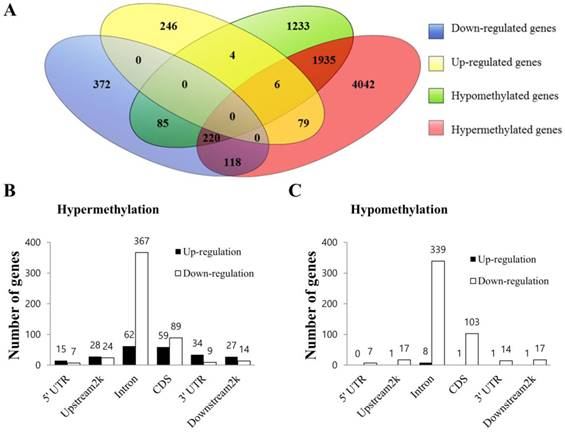
\includegraphics[width=0.8\textwidth]{journal-of-cancer_sample-result}}
% 	\caption{یک نمونه نمودار خلاصه برای نمایش نوآوری در نتایج
% 		%\cite{kim2016integrated}
% 	}
% 	\label{fig:sampleDiagram}
% \end{figure}\\
% طبیعتاً به صلاحدید نگارنده، شکل‌ها و نمودار‌ها می توانند در بخش های مختلف، خصوصا فصل
% \ref{chap:results}
% مورد استفاده قرار گیرند.

\subsection{تعریف واژه‌ها (اختیاری)}
% در این قسمت محقق باید واژه‌هایی را که ممکن است برای خواننده آشنا نباشد، تعریف کند.

\subsection{خلاصه فصل‌ها}
% در آخرین قسمتِ فصل اول پایان‌نامه، خلاصه‌ای اشاره‌وار از فصل‌های آتی آورده می‌شود تا خواننده بتواند تصویری واضح از دیگر قسمت‌های پایان‌نامه در ذهن خود ترسیم کند.

\section{جمع‌بندی}
% در این فصل به دو مقولهٔ نحوه استفاده از قالب \پ دانشگاه تهران و نیز ویژگی‌هایی که محتویات فصل اول پایان‌نامه (یعنی مقدمه) باید داشته باشند، پرداخته شد. با توجه به اینکه این راهنما نحوه استفاده از قالب را شرح داده، ملزومات محتوایی هر فصل پایان‌نامه را توضیح می‌دهد و در پیوست‌ها نیز نحوهٔ کار با لاتک را یادآوری خواهد کرد، بنابراین مطالعهٔ کامل آن مقداری وقت شما را خواهد گرفت؛ اما مطمئن باشید از اتلاف وقت شما در ادامه کارتان تا حد زیادی جلوگیری خواهد کرد. در نوشتن متن حاضر سعی شده است علاوه بر ایجاد یک قالب لاتک برای پایان‌نامه‌های دانشگاه تهران، نکات محتوایی هر فصل نیز گوشزد گردد. طبیعتاً برای نگارش پایان‌نامهٔ خود می‌بایست مطالب تمام فصل‌ها را خودتان بازنویسی کنید.

% در ادامهٔ این راهنما، تنها فصل‌هایی که یک پایان‌نامه باید داشته باشد و نیز خصوصیات یا ساختاری که محتویات هر فصل باید از آنها برخوردار باشد%
% \footnote{از روی فایل «تمپلیت نگارش و تدوین پایان‌نامه \cite{UTThesisGuide}»}،
% آورده می‌شوند. نهایتاً  در پیوست‌ها، مطالبی در باب یادآوری دستورات لاتک، نحوه نوشتن فرمول‌ها، تعاریف، قضایا، مثال‌ها، درج تصاویر، نمودارها، جداول و الگوریتم‌ها و نیز مدیریت مراجع، آمده است.

% همچنین توصیه اکید دارم که رفع خطاهایی که احتمالاً با آنها مواجه می‌شوید را به آخر موکول نفرمایید و به محض برخورد با خطا، آن را اشکال‌زدایی و برطرف نمائید.!
% و
% \verb!% !TeX root=main.tex
\chapter{مروری بر مطالعات انجام شده}
%\thispagestyle{empty} 
\section{مقدمه}
% هدف از اين فصل که با عنوان‌های  «مروری بر ادبیات موضوع%
% \LTRfootnote{Literature Review}»،
% «مروری بر منابع» و يا «مروری بر پیشینه تحقیق%
% \LTRfootnote{Background Research}»
% معرفی می‌شود، بررسی و طبقه‌بندی یافته‌های تحقیقات دیگر محققان در سطح دنیا و تعیین و شناسایی خلأهای تحقیقاتی است. آنچه را که تحقیق شما به دانش موجود اضافه می‌کند، مشخص کنید. طرح پیشینه تحقیق%
% \LTRfootnote{Background Information}
% یک مرور محققانه است و تا آنجا باید پیش برود که پیش‌زمینهٔ تاریخی مناسبی از تحقیق را بیان کند و جایگاه تحقیق فعلی را در میان آثار پیشین نشان دهد. برای این منظور منابع مرتبط با تحقیق را بررسی کنید، البته نه آنچنان گسترده که کل پیشینه تاریخی بحث را در برگیرد. برای نوشتن این بخش:
% \begin{itemize}
% 	\item
% 	دانستنی‌های موجود و پیش‌زمینهٔ تاریخی و وضعیت کنونی موضوع را چنان بیان کنید که خواننده بدون مراجعه به منابع پیشین، نتایج حاصل از مطالعات قبلی را درک و ارزیابی کند.
% 	\item
% 	نشان دهید که بر موضوع احاطه دارید. پرسش تحقیق را همراه بحث و جدل‌ها و مسائل مطرح شده بیان کنید و مهم‌ترین تحقیق‌های انجام شده در این زمینه را معرفی نمائید.
% 	\item
% 	ابتدا مطالب عمومی‌تر و سپس پژوهش‌های مشابه با کار خود را معرفی کرده و نشان دهید که تحقیق شما از چه جنبه‌ای با کار دیگران تشابه یا تفاوت دارد.
% 	\item
% 	اگر کارهای قبلی را خلاصه کرده‌اید، از پرداختن به جزئیات غیرضروری بپرهیزید. در عوض، بر یافته‌ها و مسائل روش‌شناختی مرتبط و نتایج اصلی تأکید کنید و اگر بررسی‌ها و منابع مروری عمومی دربارهٔ موضوع موجود است، خواننده را به آنها ارجاع دهید.
% \end{itemize}


% \section{مروری بر ادبیات موضوع}
% در این قسمت باید به کارهای مشابه دیگران در گذشته اشاره کرد و وزن بیشتر این قسمت بهتر است به مقالات ژورنالی سال‌های اخیر (۲ تا ۳ سال) تخصیص داده شود. به نتایج کارهای دیگران با ذکر دقیق مراجع باید اشاره شده و جایگاه و تفاوت تحقیق شما نیز با کارهای دیگران مشخص شود. استفاده از مقالات ژورنال‌های معتبر در دو یا سه سال اخیر، می‌تواند به اعتبار کار شما بیافزاید.

% \section{نتیجه‌گیری}
% ‌در نتیجه‌گیری آخر این فصل، با توجه به بررسی انجام شده بر روی مراجع تحقيق، بخش‌های قابل گسترش و تحقیق در آن حیطه و چشم‌اندازهای تحقیق مورد بررسی قرار می‌گیرند.	در برخی از تحقیقات، نتیجه نهایی فصل روش تحقیق، ارائهٔ یک چارچوب کار تحقیقی 
% \lr{(research framework)}
% است.
\ifExperimentalAuction
	تصمیم‌گیری های ما نمایشگر ارزشگذاری‌های ما هستند. اقتصاد‌دان‌ها
	\textit{ارزش اقتصادی}
	\LTRfootnote{economic value}
	این تصمیمات را با نرخی که فرد یک محصول یا دارایی را با  دیگری مبادله می کند ، بیان می‌کنند.
	این نرخ به وسیله
	\textit{تمایل به پرداخت }
	\LTRfootnote{willingness to pay}
	حداکثری فرد اندازه‌گیری می‌شود.
	\citep{luskExperimentalAuctionsMethods2007}
	\section{تعاریف، اصول و مبانی نظری}
	% این قسمت ارائهٔ خلاصه‌ای از دانش کلاسیک موضوع است. این بخش الزامی نیست و بستگی به نظر استاد راهنما دارد.

\fi

\ifTheEffectsOfDifferentPersonalData
	\textit{چاو، اوی و هربلاند}
	\LTRfootnote{Chua, H.N., J.S. Ooi, and A. Herbland}
	در سال ۲۰۲۱ اطلاعات شخصی را در ۶ دسته طبقه بندی کرده‌اند.
	\citep{chuaEffectsDifferentPersonal2021}
	جدول
	\eqref{tab:PICatAndChar}
	\begin{table}[ht]
		\caption{دسته‌ها و ویژگی‌های اطلاعت شخصی}
		\label{tab:PICatAndChar}
		\centering
		\onehalfspacing
		% \begin{tabular}{p{0.35\linewidth} | p{0.6\linewidth}}  
		\begin{tabularx}{\linewidth}{ r X }
			% \hline 
			دسته
			 &
			% درجه آزادی 
			% تبدیل مختصات &
			توضیح
			\\
			\hline
			سبک زندگی-رفتار(LB)
			 &
			% zotero://select/library/items/LCYS3GQ2
			% https://www.zotero.org/users/5038267/items/LCYS3GQ2
			%توضیح
			اطلاعت درباره ویژگی‌ها و سبک زندگی فرد که بر رابطه عاطفی یا
			اجتماعی، ترجیهات، عادات، باورها، یا دیدگاه‌های او اثر می‌گذارد.
			% مثال‌ها:
			% \lr{L1}:
			% باور
			% (
			% مانند باورهای مذهبی، باورهای فلسفی، افکار و غیره
			% )
			% % \hline 
			% \lr{L2}:
			% ترجیهات و علایق
			% (مانند نظرات، تمایلات، علایق، غذاهای مورد علاقه، رنگ‌ها، چیزهای
			% دوست‌داشتنی و دوست‌نداشتنی)
			% \lr{L3}:
			% رفتار
			% (مانند رفتار وبگردی، الگوی تماس‌ها، لینک‌های کلیک شده،
			% سبک زندگی رویکرد و غیره)
			% \lr{L4}:
			% خانواده/روابط عاطفی
			% (مانند ساختار خانواده، همشیرها، فرزندان، ازدواج‌ها، طلاق‌ها،
			% روابط عاطفی و غیره)
			\\
			اجتماعی-اقتصادی(SE)
			 &
			% ۳ & 
			% ویژگی دو &
			اطلاعاتی که سطح زندگی اقتصادی یا اجتماعی فرد را نشان می‌دهند یا
			می‌توان به وسیله این اطلاعات ویژگی‌های مزبور را استخراج کرد.
			% مثال‌ها;
			% \lr{S1}:
			% \lr{S1}:
			% \lr{S1}:
			\\
			ردیابی(T)
			 &
			اطلاعاتی که روش‌هایی را برای موقعیت‌یابی و تماس با فرد ایجاد می کند.
			% \hline 
			\\
			اقتصادی(F)
			 &
			اطلاعاتی که درآمد، حساب‌های مالی، اعتبار، توانایی خرید/خرج کردن، و
			دارایی‌های مورد تملک/اجاره شده/قرض گرفته شده را مشخص می کند.
			\\
			احراز هویت(A)
			 &
			اطلاعاتی که برای احراز هویت فرد به کار می‌روند.
			\\
			پزشکی-سلامت(MH)
			 &
			شرایط پزشکی  یا اطلاعات مرتبط با سلامت فرد.
			\\
		\end{tabularx}
	\end{table}
	% \begin{table}[ht]
	%     \caption{مدلهای تبدیل دیگر.}
	%     \label{tab:motionModelsCont}
	%     \centering
	%     \onehalfspacing
	%     \begin{tabularx}{\textwidth}{|r|c|l|X|}
	%         \hline نام مدل & درجه آزادی & تبدیل مختصات & توضیح \\ 
	%         \hline مشابهت & ۴ & $\begin{aligned} x'=sx\cos\theta - sy\sin\theta+t_x \\ y'=sx\sin\theta+sy\cos\theta+t_y  \end{aligned}$  & اقلیدسی+تغییرمقیاس \\ 		
	%         \hline آفین & ۶ & $\begin{aligned} x'=a_{11}x+a_{12}y+t_x \\ y'=a_{21}x+a_{22}y+t_y \end{aligned}$  & مشابهت+اریب‌شدگی \\
	%         \hline
	%     \end{tabularx}
	% \end{table}


	از سوی دیگر
\fi %TheEffectsOfDifferentPersonalData
\ifMultidimensionalNatureOfPrivacyRisksConceptualisationMeasurementAndImplicationsForDigitalServices
	در سال ۲۰۲۲
	\textit{
		\gls{Sabrina Karwatzki, Manuel Trenz and Daniel Veit}
	}
	 یک دسته‌بندی قاعده‌گرا
	\textit{
		\gls{Nomological}
	}
	و جامع از نگرانی‌های حریم خصوصی افراد بر اساس پژوهش های گذشته ارائه داده و اعتبار و روایی آن‌را مورد سنجش قرار‌داده‌اند
	\citep{karwatzkiMultidimensionalNaturePrivacy}
	\!.
	آنها ۷ دسته
	\textbf{
		خطر حریم خصوصی فیزیکی
		\lr{(PH)}
		\LTRfootnote{Physical privacy risk}
		،
		خطر حریم خصوصی اجتماعی
		\lr{(SO)}
		\LTRfootnote{Social privacy risk}
		،
		خطر حریم خصوصی مرتبط با منابع
		\lr{(RE)}
		\LTRfootnote{Resource-related privacy risk}
		،
		خطر حریم خصوصی روانشناختی
		\lr{(PS)}
		\LTRfootnote{Psychological privacy risk}
		،
		خطر حریم خصوصی مرتبط با تعقیب قانونی
		\lr{(PR)}
		\LTRfootnote{Prosecution-related privacy risk}
		،
		خطر حریم خصوصی مرتبط با شغل
		\lr{(CR)}
		\LTRfootnote{Career-related privacy risks}
		\textmd{و}
		خطر حریم خصوصی مرتبط با آزادی
		\lr{(FR)}
		\LTRfootnote{Freedom-related privacy risk}
	}
\fi %\ifMultidimensionalNatureOfPrivacyRisksConceptualisationMeasurementAndImplicationsForDigitalServices
را شناسایی کردند. ما
از این دسته‌بندی و توصیفاتی که در این پژوهش با دسته‌بندی‌های نامبرده مرتبط دانسته شده اند، استفاده کردیم.
!
% را در فایل 
% \lr{main.tex}،
% غیرفعال%
% \footnote{
% برای غیرفعال کردن یک دستور، کافی است در ابتدای آن، علامت درصد انگلیسی (\%) بگذارید.
% }
%  کنید. در غیر این صورت، ابتدا مطالب دو فصل اول پردازش شده و سپس مطالب فصل ۳ پردازش می‌شود که این کار باعث طولانی شدن زمان پردازش می‌گردد. هر زمان که خروجی کل \پ را خواستید، تمام فصل‌ها را دوباره در
% \lr{main.tex}
% فعال نمائید.
% بدیهتاً لازم نیست فصل‌های \پ را به ترتیب تایپ کنید. مثلاً می‌توانید ابتدا مطالب فصل ۳ را تایپ نموده و سپس مطالب فصل ۱ را تایپ کنید. 
% \subsubsection{مراجع}
% برای وارد کردن مراجع \پ کافی است فایل 
% \lr{MyReferences.bib}
% را باز کرده و مراجع خود را به شکل اقلام نمونهٔ داخل آن، وارد کنید.  سپس از \lr{bibtex} برای تولید مراجع با قالب مناسب استفاده نمائید. برای توضیحات بیشتر بخش \ref{Sec:Ref} از پیوست \ref{app:latexIntro} و نیز پیوست \ref{app:refMan} را ببینید.

% \subsubsection{واژه‌نامه فارسی به انگلیسی و برعکس}
% برای وارد کردن معادل فارسی اصطلاحات لاتین در متن و تهیه فهرست واژه‌نامه از آنها، از بستهٔ
% \lr{glossaries}
% و نرم‌افزار
% \lr{xindy}
% استفاده می‌شود. بدین منظور کافی است اصطلاحات لاتین و ترجمهٔ آنها را در فایل
% \lr{words.tex}
% وارد کرده و هر جای متن که خواستید با دستورات
% \verb|gls{label}|
% یا \verb|glspl{label}|
% معادل فارسی مفرد یا جمع یک اصطلاح را بیاورید.

% مثلا در اینجا، واژهٔ
% «\gls{Action}»
% برای بار اول و دوباره
% «\gls{Action}»
% برای بار دوم در متن ظاهر شده است.
% جهت توضیحات بیشتر به پیوست
% \ref{app:refMan}
% مراجعه کنید.
% \subsubsection{نمایه}
% برای وارد کردن نمایه، باید از 
% \lr{xindy}
% استفاده کنید. 
%زیرا 
%\lr{MakeIndex}
%با حروف «گ»، «چ»، «پ»، «ژ» و «ک» مشکل دارد و ترتیب الفبایی این حروف را رعایت نمی‌کند. همچنین، فاصله بین هر گروه از کلمات در 
%\lr{MakeIndex}،
%به درستی رعایت نمی‌شود که باعث زشت شدن حروف‌چینی این قسمت می‌شود. 
% راهنمای چگونگی کار با 
% \lr{xindy} 
% را می‌توانید در ویکی پارسی‌لاتک و یا مثالهای موجود در دی‌وی‌دی «مجموعه پارسی‌لاتک»، پیدا کنید.

% \subsection{اگر سوالی داشتم، از کی بپرسم؟}
% برای پرسیدن سوال‌های خود موقع حروف‌چینی با زی‌پرشین، می‌توانید به
% \href{http://qa.parsilatex.com}{سایت پرسش و پاسخ پارسی‌لاتک}%
% \LTRfootnote{http://qa.parsilatex.com}
% یا
% \href{http://forum.parsilatex.com}{بایگانی تالارگفتگوی قدیمی پارسی‌لاتک}%
% \mypagestye{http://forum.parsilatex.com}
% مراجعه کنید. شما هم می‌توانید روزی به سوال‌های دیگران در اینترنت جواب دهید.
% بستهٔ زی‌پرشین و بسیاری از بسته‌های مرتبط با آن مانند
% \lr{bidi} و
% \lr{Persian-bib}،
% مجموعه پارسی‌لاتک، مثالهای مختلف موجود در آن، قالب پایان‌نامه دانشگاههای مختلف و سایت پارسی‌لاتک همه به صورت داوطلبانه توسط افراد گروه پارسی‌لاتک و گروه
% \lr{Persian TeX}
% و بدون هیچ کمک مالی انجام شده‌اند. کار اصلی نوشتن و توسعه زی‌پرشین توسط آقای وفا خلیقی انجام شده است که این کار بزرگ را به انجام رساندند.
% اگر مایل به کمک به گروه پارسی‌لاتک هستید به سایت این گروه مراجعه فرمایید:
% \begin{center}
% 	\url{http://www.parsilatex.com}
% \end{center}

% \section{محتویات فصل اول یک پایان‌نامه}
% فصل اول یک پایان‌نامه باید به مقدمه یا کلیات تحقیق بپردازد.
% هدف از فصل مقدمه%
% \LTRfootnote{Introduction}،
% شرح مختصر مسأله تحقیق، اهمیت و انگیزه محقق از پرداختن به آن موضوع، بهمراه اشاره‌ای كوتاه به روش و مراحل تحقیق است. مقدمه، اولين فصل از ساختار اصلی \پ بوده و زمینه اطلاعاتی لازم را برای خواننده فراهم می‌آورد. در طول مقدمه باید سعی شود موضوع تحقیق با زبانی روشن، ساده و بطور عمیق و هدفمند به خواننده معرفی شود. این فصل باید خواننده را مجذوب و اهميت موضوع تحقيق را آشکار سازد. در مقدمه باید با ارائهٔ سوابق، شواهد تحقيقی و اطلاعات موجود (با ذکر منبع) با روشی منظم، منطقی و هدف‌دار، خواننده را جهت داد و به سوی راه حل مورد نظر هدايت کرد. مقدمه مناسب‌ترين جا برای ارائهٔ اختصارات و بعضی توضيحات کلی است، توضيحاتی که شايد نتوان در مباحث ديگر آنها را شرح داد.

% مقدمه، یکی از ارکان اساسی و اصلی پایان نامه است که مهمترین قسمت‌های آن عبارتند از: 

% \subsection{عنوان تحقیق} 
% باید شناختی دقیق و روشن از حوزهٔ موضوع تحقیق را عرضه دارد و خالی از هرگونه ابهام و پیچیدگی باشد.

% \subsection{مسأله تحقیق}
% وظیفه اصلی مقدمه بیان این مطلب به خواننده است که چرا انجام تحقیق را به عهده گرفته‌اید. اگر دلیل شما برای انجام این کار پاسخگویی به سؤال مورد علاقه‌تان است، با مشکل زیادی روبه‌رو نخواهید بود. یکی از بهترین روش‌ها برای نوشتن مقدمهٔ یک پایان‌نامه، طرح پرسش یا پرسش‌هایی مهم و اساسی است که کار تحقیقاتی شما از آغاز تا پایان قصد پاسخ دادن به آن را دارد. گاهی می‌توانید ابتدا اهمیت موضوع را بیان و سپس پرسش خود را در آن موضوع مطرح کنید.

% \subsection{تاریخچه‌ای از موضوع تحقیق}
% به طور کلی تشریح روندهای تحقیقاتی در محدودهٔ مورد مطالعه، مستلزم ارجاع به کارهای دیگران است. بعضی از نویسندگان برای کارهای دیگران هیچ اعتباری قائل نمی‌شوند و در مقابل، بعضی دیگر از نویسندگان در توصیف کارهای دیگران، بسیار زیاده‌روی می‌کنند. اکثر مواقع، ارجاع به مقالات دو سال قبل از کارتان، بهتر از نوشتن سطرهای مرجع است. در این قسمت باید به طور مختصر به نظرات و تحقیقات مربوط به موضوع و یا مسائل و مشکلات حل نشده در این حوزه و همچنین توجه و علاقه جامعه به این موضوع، اشاره شود.

% \subsection{تعریف موضوع تحقیق}
% در این قسمت محقق، موضوع مورد علاقه و یا نیاز احساس شدهٔ خود را در حوزه تحقیق بیان می‌دارد و عوامل موجود در موقعیت را تعریف و تعیین می‌کند.

% \subsection{هدف یا هدف‌های کلی و آرمانی تحقیق}
% این قسمت باید با جملات مثبت و کلی طرح شود و از طولانی شدن مطالب پرهیز شود.

% \subsection{روش انجام تحقیق}
% در این قسمت، پژوهشگر روش کاری خود را بیان می‌دارد و شیوه‌های گوناگونی را که در گردآوری مطالب خود بکار برده، ذکر می‌کند. همچنین اگر روش آماری خاصی را در تهیه و تدوین اطلاعات به کار برده است، آن شیوه را نیز اینجا بیان می‌کند.

% \subsection{نوآوری، اهمیت و ارزش تحقیق}
% در این قسمت، در مورد نوآوری علمی و عملی تحقیق که محقق به آن دست خواهد یافت، بحث می‌شود. ممکن است لازم باشد تا برخی نمودارهای خلاصه در این بخش استفاده شوند. به عنوان مثال، نموداری از مقاله
% \cite{kim2016integrated}
% در شکل
% \ref{fig:sampleDiagram}
% آمده است.
% \begin{figure}[ht]
% 	\centerline{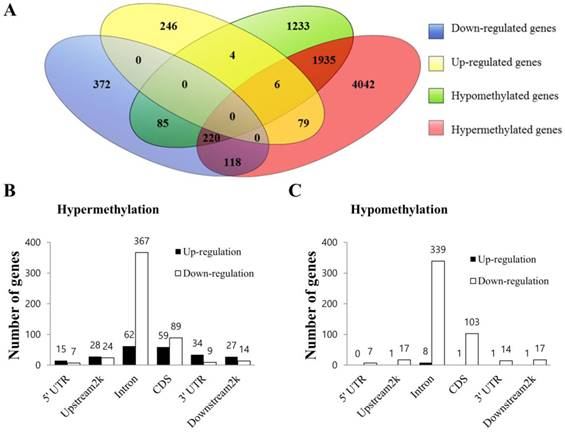
\includegraphics[width=0.8\textwidth]{journal-of-cancer_sample-result}}
% 	\caption{یک نمونه نمودار خلاصه برای نمایش نوآوری در نتایج
% 		%\cite{kim2016integrated}
% 	}
% 	\label{fig:sampleDiagram}
% \end{figure}\\
% طبیعتاً به صلاحدید نگارنده، شکل‌ها و نمودار‌ها می توانند در بخش های مختلف، خصوصا فصل
% \ref{chap:results}
% مورد استفاده قرار گیرند.

\subsection{تعریف واژه‌ها (اختیاری)}
% در این قسمت محقق باید واژه‌هایی را که ممکن است برای خواننده آشنا نباشد، تعریف کند.

\subsection{خلاصه فصل‌ها}
% در آخرین قسمتِ فصل اول پایان‌نامه، خلاصه‌ای اشاره‌وار از فصل‌های آتی آورده می‌شود تا خواننده بتواند تصویری واضح از دیگر قسمت‌های پایان‌نامه در ذهن خود ترسیم کند.

\section{جمع‌بندی}
% در این فصل به دو مقولهٔ نحوه استفاده از قالب \پ دانشگاه تهران و نیز ویژگی‌هایی که محتویات فصل اول پایان‌نامه (یعنی مقدمه) باید داشته باشند، پرداخته شد. با توجه به اینکه این راهنما نحوه استفاده از قالب را شرح داده، ملزومات محتوایی هر فصل پایان‌نامه را توضیح می‌دهد و در پیوست‌ها نیز نحوهٔ کار با لاتک را یادآوری خواهد کرد، بنابراین مطالعهٔ کامل آن مقداری وقت شما را خواهد گرفت؛ اما مطمئن باشید از اتلاف وقت شما در ادامه کارتان تا حد زیادی جلوگیری خواهد کرد. در نوشتن متن حاضر سعی شده است علاوه بر ایجاد یک قالب لاتک برای پایان‌نامه‌های دانشگاه تهران، نکات محتوایی هر فصل نیز گوشزد گردد. طبیعتاً برای نگارش پایان‌نامهٔ خود می‌بایست مطالب تمام فصل‌ها را خودتان بازنویسی کنید.

% در ادامهٔ این راهنما، تنها فصل‌هایی که یک پایان‌نامه باید داشته باشد و نیز خصوصیات یا ساختاری که محتویات هر فصل باید از آنها برخوردار باشد%
% \footnote{از روی فایل «تمپلیت نگارش و تدوین پایان‌نامه \cite{UTThesisGuide}»}،
% آورده می‌شوند. نهایتاً  در پیوست‌ها، مطالبی در باب یادآوری دستورات لاتک، نحوه نوشتن فرمول‌ها، تعاریف، قضایا، مثال‌ها، درج تصاویر، نمودارها، جداول و الگوریتم‌ها و نیز مدیریت مراجع، آمده است.

% همچنین توصیه اکید دارم که رفع خطاهایی که احتمالاً با آنها مواجه می‌شوید را به آخر موکول نفرمایید و به محض برخورد با خطا، آن را اشکال‌زدایی و برطرف نمائید.		% فصل اول: مقدمه
% % !TeX root=main.tex
\chapter{مروری بر مطالعات انجام شده}
%\thispagestyle{empty} 
\section{مقدمه}
% هدف از اين فصل که با عنوان‌های  «مروری بر ادبیات موضوع%
% \LTRfootnote{Literature Review}»،
% «مروری بر منابع» و يا «مروری بر پیشینه تحقیق%
% \LTRfootnote{Background Research}»
% معرفی می‌شود، بررسی و طبقه‌بندی یافته‌های تحقیقات دیگر محققان در سطح دنیا و تعیین و شناسایی خلأهای تحقیقاتی است. آنچه را که تحقیق شما به دانش موجود اضافه می‌کند، مشخص کنید. طرح پیشینه تحقیق%
% \LTRfootnote{Background Information}
% یک مرور محققانه است و تا آنجا باید پیش برود که پیش‌زمینهٔ تاریخی مناسبی از تحقیق را بیان کند و جایگاه تحقیق فعلی را در میان آثار پیشین نشان دهد. برای این منظور منابع مرتبط با تحقیق را بررسی کنید، البته نه آنچنان گسترده که کل پیشینه تاریخی بحث را در برگیرد. برای نوشتن این بخش:
% \begin{itemize}
% 	\item
% 	دانستنی‌های موجود و پیش‌زمینهٔ تاریخی و وضعیت کنونی موضوع را چنان بیان کنید که خواننده بدون مراجعه به منابع پیشین، نتایج حاصل از مطالعات قبلی را درک و ارزیابی کند.
% 	\item
% 	نشان دهید که بر موضوع احاطه دارید. پرسش تحقیق را همراه بحث و جدل‌ها و مسائل مطرح شده بیان کنید و مهم‌ترین تحقیق‌های انجام شده در این زمینه را معرفی نمائید.
% 	\item
% 	ابتدا مطالب عمومی‌تر و سپس پژوهش‌های مشابه با کار خود را معرفی کرده و نشان دهید که تحقیق شما از چه جنبه‌ای با کار دیگران تشابه یا تفاوت دارد.
% 	\item
% 	اگر کارهای قبلی را خلاصه کرده‌اید، از پرداختن به جزئیات غیرضروری بپرهیزید. در عوض، بر یافته‌ها و مسائل روش‌شناختی مرتبط و نتایج اصلی تأکید کنید و اگر بررسی‌ها و منابع مروری عمومی دربارهٔ موضوع موجود است، خواننده را به آنها ارجاع دهید.
% \end{itemize}


% \section{مروری بر ادبیات موضوع}
% در این قسمت باید به کارهای مشابه دیگران در گذشته اشاره کرد و وزن بیشتر این قسمت بهتر است به مقالات ژورنالی سال‌های اخیر (۲ تا ۳ سال) تخصیص داده شود. به نتایج کارهای دیگران با ذکر دقیق مراجع باید اشاره شده و جایگاه و تفاوت تحقیق شما نیز با کارهای دیگران مشخص شود. استفاده از مقالات ژورنال‌های معتبر در دو یا سه سال اخیر، می‌تواند به اعتبار کار شما بیافزاید.

% \section{نتیجه‌گیری}
% ‌در نتیجه‌گیری آخر این فصل، با توجه به بررسی انجام شده بر روی مراجع تحقيق، بخش‌های قابل گسترش و تحقیق در آن حیطه و چشم‌اندازهای تحقیق مورد بررسی قرار می‌گیرند.	در برخی از تحقیقات، نتیجه نهایی فصل روش تحقیق، ارائهٔ یک چارچوب کار تحقیقی 
% \lr{(research framework)}
% است.
\ifExperimentalAuction
	تصمیم‌گیری های ما نمایشگر ارزشگذاری‌های ما هستند. اقتصاد‌دان‌ها
	\textit{ارزش اقتصادی}
	\LTRfootnote{economic value}
	این تصمیمات را با نرخی که فرد یک محصول یا دارایی را با  دیگری مبادله می کند ، بیان می‌کنند.
	این نرخ به وسیله
	\textit{تمایل به پرداخت }
	\LTRfootnote{willingness to pay}
	حداکثری فرد اندازه‌گیری می‌شود.
	\citep{luskExperimentalAuctionsMethods2007}
	\section{تعاریف، اصول و مبانی نظری}
	% این قسمت ارائهٔ خلاصه‌ای از دانش کلاسیک موضوع است. این بخش الزامی نیست و بستگی به نظر استاد راهنما دارد.

\fi

\ifTheEffectsOfDifferentPersonalData
	\textit{چاو، اوی و هربلاند}
	\LTRfootnote{Chua, H.N., J.S. Ooi, and A. Herbland}
	در سال ۲۰۲۱ اطلاعات شخصی را در ۶ دسته طبقه بندی کرده‌اند.
	\citep{chuaEffectsDifferentPersonal2021}
	جدول
	\eqref{tab:PICatAndChar}
	\begin{table}[ht]
		\caption{دسته‌ها و ویژگی‌های اطلاعت شخصی}
		\label{tab:PICatAndChar}
		\centering
		\onehalfspacing
		% \begin{tabular}{p{0.35\linewidth} | p{0.6\linewidth}}  
		\begin{tabularx}{\linewidth}{ r X }
			% \hline 
			دسته
			 &
			% درجه آزادی 
			% تبدیل مختصات &
			توضیح
			\\
			\hline
			سبک زندگی-رفتار(LB)
			 &
			% zotero://select/library/items/LCYS3GQ2
			% https://www.zotero.org/users/5038267/items/LCYS3GQ2
			%توضیح
			اطلاعت درباره ویژگی‌ها و سبک زندگی فرد که بر رابطه عاطفی یا
			اجتماعی، ترجیهات، عادات، باورها، یا دیدگاه‌های او اثر می‌گذارد.
			% مثال‌ها:
			% \lr{L1}:
			% باور
			% (
			% مانند باورهای مذهبی، باورهای فلسفی، افکار و غیره
			% )
			% % \hline 
			% \lr{L2}:
			% ترجیهات و علایق
			% (مانند نظرات، تمایلات، علایق، غذاهای مورد علاقه، رنگ‌ها، چیزهای
			% دوست‌داشتنی و دوست‌نداشتنی)
			% \lr{L3}:
			% رفتار
			% (مانند رفتار وبگردی، الگوی تماس‌ها، لینک‌های کلیک شده،
			% سبک زندگی رویکرد و غیره)
			% \lr{L4}:
			% خانواده/روابط عاطفی
			% (مانند ساختار خانواده، همشیرها، فرزندان، ازدواج‌ها، طلاق‌ها،
			% روابط عاطفی و غیره)
			\\
			اجتماعی-اقتصادی(SE)
			 &
			% ۳ & 
			% ویژگی دو &
			اطلاعاتی که سطح زندگی اقتصادی یا اجتماعی فرد را نشان می‌دهند یا
			می‌توان به وسیله این اطلاعات ویژگی‌های مزبور را استخراج کرد.
			% مثال‌ها;
			% \lr{S1}:
			% \lr{S1}:
			% \lr{S1}:
			\\
			ردیابی(T)
			 &
			اطلاعاتی که روش‌هایی را برای موقعیت‌یابی و تماس با فرد ایجاد می کند.
			% \hline 
			\\
			اقتصادی(F)
			 &
			اطلاعاتی که درآمد، حساب‌های مالی، اعتبار، توانایی خرید/خرج کردن، و
			دارایی‌های مورد تملک/اجاره شده/قرض گرفته شده را مشخص می کند.
			\\
			احراز هویت(A)
			 &
			اطلاعاتی که برای احراز هویت فرد به کار می‌روند.
			\\
			پزشکی-سلامت(MH)
			 &
			شرایط پزشکی  یا اطلاعات مرتبط با سلامت فرد.
			\\
		\end{tabularx}
	\end{table}
	% \begin{table}[ht]
	%     \caption{مدلهای تبدیل دیگر.}
	%     \label{tab:motionModelsCont}
	%     \centering
	%     \onehalfspacing
	%     \begin{tabularx}{\textwidth}{|r|c|l|X|}
	%         \hline نام مدل & درجه آزادی & تبدیل مختصات & توضیح \\ 
	%         \hline مشابهت & ۴ & $\begin{aligned} x'=sx\cos\theta - sy\sin\theta+t_x \\ y'=sx\sin\theta+sy\cos\theta+t_y  \end{aligned}$  & اقلیدسی+تغییرمقیاس \\ 		
	%         \hline آفین & ۶ & $\begin{aligned} x'=a_{11}x+a_{12}y+t_x \\ y'=a_{21}x+a_{22}y+t_y \end{aligned}$  & مشابهت+اریب‌شدگی \\
	%         \hline
	%     \end{tabularx}
	% \end{table}


	از سوی دیگر
\fi %TheEffectsOfDifferentPersonalData
\ifMultidimensionalNatureOfPrivacyRisksConceptualisationMeasurementAndImplicationsForDigitalServices
	در سال ۲۰۲۲
	\textit{
		\gls{Sabrina Karwatzki, Manuel Trenz and Daniel Veit}
	}
	 یک دسته‌بندی قاعده‌گرا
	\textit{
		\gls{Nomological}
	}
	و جامع از نگرانی‌های حریم خصوصی افراد بر اساس پژوهش های گذشته ارائه داده و اعتبار و روایی آن‌را مورد سنجش قرار‌داده‌اند
	\citep{karwatzkiMultidimensionalNaturePrivacy}
	\!.
	آنها ۷ دسته
	\textbf{
		خطر حریم خصوصی فیزیکی
		\lr{(PH)}
		\LTRfootnote{Physical privacy risk}
		،
		خطر حریم خصوصی اجتماعی
		\lr{(SO)}
		\LTRfootnote{Social privacy risk}
		،
		خطر حریم خصوصی مرتبط با منابع
		\lr{(RE)}
		\LTRfootnote{Resource-related privacy risk}
		،
		خطر حریم خصوصی روانشناختی
		\lr{(PS)}
		\LTRfootnote{Psychological privacy risk}
		،
		خطر حریم خصوصی مرتبط با تعقیب قانونی
		\lr{(PR)}
		\LTRfootnote{Prosecution-related privacy risk}
		،
		خطر حریم خصوصی مرتبط با شغل
		\lr{(CR)}
		\LTRfootnote{Career-related privacy risks}
		\textmd{و}
		خطر حریم خصوصی مرتبط با آزادی
		\lr{(FR)}
		\LTRfootnote{Freedom-related privacy risk}
	}
\fi %\ifMultidimensionalNatureOfPrivacyRisksConceptualisationMeasurementAndImplicationsForDigitalServices
را شناسایی کردند. ما
از این دسته‌بندی و توصیفاتی که در این پژوهش با دسته‌بندی‌های نامبرده مرتبط دانسته شده اند، استفاده کردیم.
		% فصول دوم: مروری بر مطالعات انجام شده
% % !TeX root=main.tex
\chapter{روش تحقیق}
%\thispagestyle{empty} 
\section{نوع پژوهش}
پژوهش حاضر از نوع توصیفی-همبستگی است.
\section{تعریف متغیر‌ها}
% ^ %%%%%%%%%%%%%%%%%%%%%%%%%%%%%%%%%%%%%%%%%%%%%%%%%%%%%%%%%%%%%
% ^ %%%%%%%%%%%%%%%%%%%%%%%%%%%%%%%%%%%%%%%%%%%%%%%%%%%%%%%%%%%%%
% ^ %%%%%%%%%%%%%%%%%%%%%%%%%%%%%%%%%%%%%%%%%%%%%%%%%%%%%%%%%%%%%

\subsection{تعریف نظری و عملیاتی مشخصات دموگرافیک}


% ^ %%%%%%%%%%%%%%%%%%%%%%%%%%%%%%%%%%%%%%%%%%%%%%%%%%%%%%%%%%%%%
% ^ %%%%%%%%%%%%%%%%%%%%%%%%%%%%%%%%%%%%%%%%%%%%%%%%%%%%%%%%%%%%%
% ^ %%%%%%%%%%%%%%%%%%%%%%%%%%%%%%%%%%%%%%%%%%%%%%%%%%%%%%%%%%%%%
\subsection{تعریف عملیاتی پارامترهای
    % نظریه رفتار برنامه ریزی شده    
    \textit{\gls{Theory of planned behavior}}
}

برای طراحی پرسشنامه جهت سنجش پارامتر‌های تشکیل دهنده ساختار
\textit{\gls{Theory of planned behavior}}
از دستور العمل ارائه شده توسط
\textit{\gls{Icek Ajzen}}
\!\cite{IcekAjzenHomepage}
استفاده شد. این پرسشنامه دارای ۴ سوال، هر یک برای اندازه‌گیری
یکی از پارامترهای نظریه فوق، است.هر سوال دارای ۵ گزینه
«کاملا موافقم»،
«نسبتا موافقم»،
«نه موافقم و نه مخالف»،
«نسبتا مخالفم»
و
«کاملا مخالفم»
به ترتیب با نمرات چهار، سه، دو، یک و صفر، می‌باشد.
برای طراحی این پرسشنامه از تحقیقی که در سال ۲۰۲۰ انجام شده است الهام گرفته شده است
\!\cite{vanderschyffInformationPrivacyBehavior2020a}.
این تحقیق جهت بررسی رفتار کاربران
\textit{\gls{Facebook}}
در نصب  کردن
\gls{App}
\!‌های
این شبکه اجتماعی انجام شده‌است. این
\gls{App}
\!‌ها
که هر یک سرویس‌های مورد علاقه کاربران را ارائه می‌کنند، می‌توانند به همه یا بخشی از اطلاعات شخصی
کاربر و دوستان او در
\gls{Facebook}
دسترسی پیدا کنند. نمونه یکی از همین
\gls{App}
\!‌ها
در سال ۲۰۱۳ توسط حدود سیصد هزار نفر از کاربران
\gls{Facebook}
نصب شد و با دسترسی پیدا کردن به پروفایل شخصی آنها و دوستان آنها،
اطلاعات هشتاد و هفت میلیون‌ نفر را استخراج کند
\cite{confessoreCambridgeAnalyticaFacebook2018,salinasZuckerbergCambridgeAnalytica,smithThereOpenSecret}.
سوء استفاده و به اشتراک گذاری مجدد این اطلاعات بعدا باعث
به وجود آمدن
\gls{Cambridge Analytica scandal}
در سال ۲۰۱۶ شد
\!\cite{gonzalezGlobalReactionsCambridge2019,SuspendingCambridgeAnalytica2018}.
سوالات طراحی شده در جدول
\eqref{tab:TPBquestions}
درج شده‌اند.

\begin{table}[ht]
    \caption{سوال‌ها و پارامتر‌های \gls{Theory of planned behavior}}
    \label{tab:TPBquestions}
    \centering
    \onehalfspacing
    % \begin{tabular}{p{0.35\linewidth} | p{0.6\linewidth}}  
    \begin{tabularx}{\linewidth}{ r X }
        % \hline 
        پارامتر
         &
        % درجه آزادی 
        % تبدیل مختصات &
        سوال
        \\
        \hline
        \gls{Atteutude}
         &
        % zotero://select/library/items/LCYS3GQ2
        % https://www.zotero.org/users/5038267/items/LCYS3GQ2
        %توضیحو
        آخرین باری که برنامه
        \gls{Whasapp}
        نصب کردم، از من درخواست کرد که
        به لیست همه اسامی و شماره تلفن‌های‌ ذخیره
        در گوشی‌ من، دسترسی داشته باشد
        \!.نظر شما چیست؟

        ۱-خیلی خوب است
        ۲-خوب است
        ۳-نه خوب است نه بد
        ۴-بد است
        ۵-خیلی بد است
        \\
        \gls{Subjective norm}
         &

        به نظر من، همه دوستانم اگر امروز برنامه
        \gls{Whasapp}
        را دوباره نصب کنند، اجازه می دهند که
        به لیست همه اسامی و شماره تلفن‌های‌ ذخیره
        در گوشی‌شان، دسترسی داشته باشد.

        چقدر از این موضوع اطمینان دارید؟

        ۱-کاملا مطمئنم
        ۲-نسبتا مطمئنم
        ۳-نظری ندارم
        ۴-زیاد مطمئنم نیستم
        ۵-اصلا مطمئنم نیستم
        % مثال‌ها;
        % \lr{S1}:
        % \lr{S1}:
        % \lr{S1}:
        \\
        \gls{Perceived Behavioral control}
         &
        اگر من امروز برنامه
        \gls{Whasapp}
        را دوباره نصب کنم، اجازه دسترسی به
        لیست اسامی و شماره تلفن های
        ذخیره در گوشی‌ام را، خواهم داد.

        آیا می‌توانید اجازه ندهید؟

        ۱-کاملا می‌توانم
        ۲-شاید بتوانم
        ۳-نمی‌دانم
        ۴-شاید نتوانم
        ۵-اصلا نمی‌توانم

        % \hline 
        \\
        \gls{Intention}
         &
        من قصد دارم که اگر امروز برنامه
        \gls{Whasapp}
        را دوباره نصب کنم و اجازه دسترسی
        به لیست اسامی و شماره تلفن های
        ذخیره در گوشی‌ام را بدهم.

        چقدر از این موضوع اطمینان دارید؟

        ۱-حتما می‌دهم
        ۲-شاید بدهم
        ۳-نمی‌دانم
        ۴-شاید ندهم
        ۵-اصلا نمی‌دهم
        % \hline 
        \\
    \end{tabularx}
\end{table}
% ^ %%%%%%%%%%%%%%%%%%%%%%%%%%%%%%%%%%%%%%%%%%%%%%%%%%%%%%%%%%%%%
% ^ %%%%%%%%%%%%%%%%%%%%%%%%%%%%%%%%%%%%%%%%%%%%%%%%%%%%%%%%%%%%%
% ^ %%%%%%%%%%%%%%%%%%%%%%%%%%%%%%%%%%%%%%%%%%%%%%%%%%%%%%%%%%%%%

\subsection{تعریف نظری متغیر جهت‌گیری ارزش اجتماعی}
\textit{
    \textbf{
        \gls{Social Value Orientations}
    }
}
عناوین مختلفی برای اشاره به انگیزه‌هایی که شالوده
\gls{Interdependent decision behavior}
را تشکیل می‌دهند، به کار برده شده است
\!:
\!,
\textit{
    \gls{Welfare tradeoff ratios}
}
\!,
\textit{
    \gls{Other-regarding preferences}
}
\!,
\textit{
    \gls{Social motives}
}
\!,
\!,
\textit{
    \gls{Social preferences}
}
و در پایان
\textit{
    \gls{Social Value Orientations}
}
\!\cite{murphyMeasuringSocialValue2011}.
تاثیر گرفتن نسبی این انگیزه‌ها از دریافتی فرد دیگر که
در پژوهش‌های مختلف نشان داده شده است، پیش‌فرض‌های
\textit{
    \gls{Rational choice theory}
}
را به چالش می‌کشند.از این پیش‌فرض‌ها با عنوان
\textit{
    \gls{Selfishness axiom}
}
نام برده شده است
\!\cite{henrichEconomicManCrosscultural2005}.

در غالب چارچوب
\gls{Social Value Orientations}
فرض می‌شود که افراد از نظر هدف یا انگیزه با یکدیگر تقاوت دارند. این
تفاوت در ارزیابی آنها در تقسیم یک دارایی میان خود
و فرد دیگر ظاهر می‌شود. به عنوان مثال ممکن است فرد تصمیم گیرنده
تلاش کند تا دریافتی خودش را حداکثر کند
\textit{
    \!(\gls{Individualistic})
}،
یا تلاش کند که دریافتی مشترک‌اش را با فرد دیگر حداکثر کند
\!(\gls{Prosocial}).
به همین ترتیب ممکن است تلاش کند تفاوت دریافتی خود و فرد دیگر را حداکثر کند
\textit{
    \!(\gls{Competitive})
}
و
یا آن‌را حداقل کند
\textit{
    \!(\gls{Inequality averse})
}.
به این ترتیب
\textit{
    \gls{Selfishness axiom}
}
به صورت یک نوع خاص از
\textit{
    \gls{Social Value Orientations}
}
در می‌آید که کاملا
\textit{
    \gls{Individualistic}
}
است. گفتنی است که فرض کردن طیف‌های متفاوتی از
\textit{
    \gls{Social Value Orientations}
}
فرض
\textit{
    \gls{Rational choice theory}
}
را به چالش نمی‌کشد بلکه به عنوان افزونه‌ای برای افزایش
\textit{
    \gls{Psychological realism}
}
و
\textit{
    \gls{Descriptive accuracy}
}
این نظریه به کار می‌رود.

نشان داده شده است که
\textit{
    \gls{Social Value Orientations}
}
بر روی
\textit{
    \gls{Cognition}
}
تاثیر می‌گذارد و سبب‌ساز ایجاد رفتار در زمینه‌های متفاوت
\textit{
    \gls{Interpersonal decision making}
}،
به ویژه در
\textit{
    \gls{Negotiation settings}
}
\!\citep{dedreuShareShareAlike1998}
و
\textit{
    \gls{Resource dilemma}
}
\!\citep{rochCognitiveLoadEquality2000,rochEffectsEnvironmentalUncertainty1997,samuelsonMultiattributeEvaluationApproach1993}
می‌گردد.
\textit{
    \gls{Social Value Orientations}
}
همچنین به عنوان
\textit{
    \gls{Covariate}
}
در تعامل با حالات  هیجانی مختلف، تمایل به همکاری را تحت تاثیر قرار می‌دهد
\citep{zeelenbergEmotionSpecificityDecision2008}.
\gls{Social Value Orientations}
در
\textit{
    \gls{Non-human primate}
}
نیز مشاهده شده است که  نشان می‌دهد، بعضی از دیگر گونه‌ها نیز رفتار
\gls{Prosocial}
از خود نشان می‌دهند.
% ^ %%%%%%%%%%%%%%%%%%%%%%%%%%%%%%%%%%%%%%%%%%%%%%%%%%%%%%%%%%%%%
% ^ %%%%%%%%%%%%%%%%%%%%%%%%%%%%%%%%%%%%%%%%%%%%%%%%%%%%%%%%%%%%%
% ^ %%%%%%%%%%%%%%%%%%%%%%%%%%%%%%%%%%%%%%%%%%%%%%%%%%%%%%%%%%%%%

\subsection{تعریف عملیاتی متغیر جهت‌گیری ارزش اجتماعی}
با توجه به محدودیت‌های ابزار‌هایی که با استفاده از
\textit{
    \gls{Categorical approach}
}
\gls{Social Value Orientations}
را می‌سنجند
(مانند عدم دقت نسبت به تقاوت های فردی آزمودنی‌ها به علت
وضوح پایین، محدود بودن به ایجاد تمایز تنها با استفاده از  تولید
\textit{
    \gls{Nominal categorization}
}
و
عدم تولید نتایج نامتناقض، نیاز به زمان و زحمت زیاد از طرف آزمودنی، عدم
حساسیت کافی برای تشخیص انگیزش‌های ظریف‌تر مانند
\gls{Inequality aversion}
)
\citep{murphyMeasuringSocialValue2011}
از
\textit{
    \gls{SVO Slider Measure}
}
استفاده کردیم. این ابزار
به تفاوت‌های درون فردی و میان فردی حساس است و مقایسه را تسهیل می‌کند
\!.
\textit{
    \gls{SVO Slider Measure}
}
قابلیت استفاده آسانی دارد، کارامد است، می تواند تفاوت‌های بیشتر متداول
فردی را تشخیص دهد،  اجازه ارزیابی رده‌بندی
\textit{
    \gls{Social preferences}
}
را می‌دهد و نتایج با معنی  بار تقریبا همه آزمودنی‌ها ایجاد می‌کند. این
ابزار به نیاز به سنجه‌های با وضوح بالا است، که داده‌های
\textit{
    \gls{Continuous}
}
تولید می‌کند.
\subsection{تعریف عملیاتی }
این ابزار به صورت یک
\textit{
    \gls{Web interface}
}
طراحی شده است
\!.
\textit{
    \gls{Source code}
}
این ابزار که به وسیله بسته  نرم‌افزاری
\textit{
    \gls{Next.js}
}
نوشته شده است به کار گرفته شد و تغییراتی به منظور فارسی کردن زبان رابط کاربری و
بهینه کردن بخش‌های مختلف آن برای استفاده در این پژوهش، در
\gls{Source code}
انجام شد.
در نهایت برای ایجاد یک تجربه پیوسته و بدون وقفه برای آزمودنی‌ها، این ابزار
در بقیه قسمتهای طراحی شده آزمایش، ادغام شد
\!.
این ابزار دارای شش بخش  اصلی و نه بخش ثانویه اختیاری است.  همه بخش‌ها شکل کلی
یکسانی دارند. هر بخش شامل یک وظیفه تصمیم گیری برای تقسیم منابع اشتراکی است. منابع
اشتراکی دارای مقادیر پیوسته هستند که به وسیله حرکت دادن
\textit{
    \gls{Slider}
}
توسط آزمودنی که فرد تصمیم گیرنده است، تغییر می‌کنند. برای مثال فرد تصمیم گیرنده
می‌تواند مقدار
$ x $
را بین ۵۰ و ۱۰۰ که شامل هر دو عدد نیز می‌شود، را انتخاب کند. دریافتی او مقدار
$ x $
خواهد بود در حالی‌که به فرد دیگر
$ 150 - x $
می‌رسد. شمارنده‌های موجود در صفحه مقادیری که در هر لحظه به دو طرف میرسد را، همراه با
جابجا شدن
\textit{
    \gls{Slider}
}
بر روی
\textit{
    \gls{Slider bar}
}
نشان می‌دهند. همزمان  دو نمودار میله‌ای افقی به صورت بصری کم و زیاد شدن
سهم طرفین را به صورت کیفی، با تغییر  اندازه نمایش می‌دهند. وقتی که
آزمودنی
\textit{
    \gls{Slider}
}
را بر روی مقدار مورد پسند خود قرار داد، می‌تواند دکمه تایید را فشار دهد تا اطلاعات این بخش ذخیره شوند
\!\citep{PdarcheSvoApplication}.

% & %%%%%%%%%%%%%%%%%%%%%%%%%%%%%%%%%%%%%%%%%%%%%%%%%%%%%%%%%%%%%
% & %%%%%%%%%%%%%%%%%%%%%%%%%%%%%%%%%%%%%%%%%%%%%%%%%%%%%%%%%%%%%
% ^ %%%%%%%%%%%%%%%%%%%%%%%بقیه اش نوشته شود%%%%%%%%%%%%%%%%%%%%%%%%%%%%%%%%%%%%%%


% ^ %%%%%%%%%%%%%%%%%%%%%%%%%%%%%%%%%%%%%%%%%%%%%%%%%%%%%%%%%%%%%
% ^ %%%%%%%%%%%%%%%%%%%%%%%%%%%%%%%%%%%%%%%%%%%%%%%%%%%%%%%%%%%%%
% ^ %%%%%%%%%%%%%%%%%%%%%%%%%%%%%%%%%%%%%%%%%%%%%%%%%%%%%%%%%%%%%
\subsection{تعریف نظری متغیر تصمیم گیری به اشتراک گذاری اطلاعات خصوصی دیگران}
افراد در موقعیت‌های زیادی با شرایط تصمیم گیری برای انتخاب میان
به اشتراک گذاری اطلاعات شخصی خود و نگه داشتن آن نزد خود، روبرو می‌شوند.
آنها در این شرایط سود و یا زیان خود را در نظر می‌گیرند
\!\cite{dinevExtendedPrivacyCalculus2006b,dienlinExtendedPrivacyCalculus2016}
\!.
تصمیم‌ گیری برای به  اشتراک گذاشتن اطلاعات شخصی دیگران، ملاحظات اجتماعی را به همراه دارد.
در این شرایط فرد تصمیم گیرنده، منفعتی که با به اشتراک گذاری اطلاعات شخصی دیگران به دست می آورد را
با کنترلی که فرد دیگر بر روی اطلاعات شخصی خود دارد و یا با
\textit{
    \gls{Information privacy}
}
سبک و سنگین می‌کند
\!
\!\cite{kamleitnerYourDataMy2019,puModelFactorsInfluencing2016}
\!.
% ^ %%%%%%%%%%%%%%%%%%%%%%%%%%%%%%%%%%%%%%%%%%%%%%%%%%%%%%%%%%%%%
% ^ %%%%%%%%%%%%%%%%%%%%%%%%%%%%%%%%%%%%%%%%%%%%%%%%%%%%%%%%%%%%%
% ^ %%%%%%%%%%%%%%%%%%%%%%%%%%%%%%%%%%%%%%%%%%%%%%%%%%%%%%%%%%%%%
% ^ %%%%%%%%%%%%%%%%%%%%%%%%%%%%%%%%%%%%%%%%%%%%%%%%%%%%%%%%%%%%%
% ^ %%%%%%%%%%%%%%%%%%%%%%%%%%%%%%%%%%%%%%%%%%%%%%%%%%%%%%%%%%%%%
% ^ %%%%%%%%%%%%%%%%%%%%%%%%%%%%%%%%%%%%%%%%%%%%%%%%%%%%%%%%%%%%%
\subsection{تعریف نظری متغیر
    \textit{هنجار ذهنی }
    و
    \textit{باور هنجاری از ارزش اطلاعات}
    خصوصی دیگران}
    \textit{
        \gls{Subjective norm}
    }
    و
    \textit{
        \gls{Normative belief}
    }
    دو مفهوم اساسی هستند که نگرش فرد نسبت به هنجار اجتماعی نسبت به یک موضوع را در 
    نظریه رفتار برنامه‌ریزی شده
    تعریف می‌کنند. 
    باور هنجاری
    ، ادراک فرد از فشار‌های هنجارهای اجتماعی،  و یا باورهای دیگران 
    به اینکه چه رفتاری باید یا نباید انجام شود. 
    هنجار ذهنی
    ادراک فرد درباره یک رفتار مشخص است که تحت تاثیر قضاوت افراد مهم زندگی 
فرد، قرار دارد. 
در اینجا رفتاری که مد نظر قرار دارد تصمیم‌گیری برای مشخص کردن مبلغ پولی که برای خرید  یک مجموعه داده مشخصی از اطلاعات 
شخصی دیگران لازم است، می‌باشد.
    \!\cite{amjadIdentifyingChangingNormative2009}
% ^ %%%%%%%%%%%%%%%%%%%%%%%%%%%%%%%%%%%%%%%%%%%%%%%%%%%%%%%%%%\!\cite{kamleitnerYourDataMy2019,amjadIdentifyingChangingNormative2009}%%%
% ^ %%%%%%%%%%%%%%%%%%%%%%%%%%%%%%%%%%%%%%%%%%%%%%%%%%%%%%%%%%%%%
% ^ %%%%%%%%%%%%%%%%%%%%%%%%%%%%%%%%%%%%%%%%%%%%%%%%%%%%%%%%%%%%%
% ^ %%%%%%%%%%%%%%%%%%%%%%%%%%%%%%%%%%%%%%%%%%%%%%%%%%%%%%%%%%%%%
% ^ %%%%%%%%%%%%%%%%%%%%%%%%%%%%%%%%%%%%%%%%%%%%%%%%%%%%%%%%%%%%%
% ^ %%%%%%%%%%%%%%%%%%%%%%%%%%%%%%%%%%%%%%%%%%%%%%%%%%%%%%%%%%%%%
\subsection{تعریف عملیاتی متغیر
    \textit{هنجار ذهنی }
    و
    \textit{باور هنجاری از ارزش اطلاعات}
    خصوصی دیگران}
برای اندازه‌گیری
\textit{
    \gls{Subjective norm about information value}
}
و
\textit{
    \gls{Normative belief about information value}
}
از پرسشنامه پژوهش‌گر ساخته
\textit{
    \gls{Dataset valuation invetory}
}
استفاده شد.
این ابزار دارای ۱۴ سوال است که دسته‌های هفت‌گانه داده‌های شخصی دیگران را مورد ارزش‌یابی قرار می‌دهد.
پژوهشی که برای یافتن ابعاد اطلاعات شخصی بر اساس نوع خطری که افراد
از فاش شدن آن احساس لحاظ می‌کنند، ۷ دسته از اطلاعات شخصی را مشخص کرده‌است
\citep{karwatzkiMultidimensionalNaturePrivacy}.
هر یک از این دسته‌ها دارای ۲ سوال در پرسشنامه هستند. برای سنجش 
پایایی درونی
این پرسشنامه سوالات به دو پرسشنامه ۷ سوالی تقسیم شدند.
هر یک از این پرسشنامه‌ها دارای یک سوال از هر یک از دسته‌های دسته‌بندی هفت‌گانه اطلاعات، می‌باشند.
به هر نیمی از افراد شرکت کننده در آزمایش، به طور تصادفی، پرسشنامه ۷ سوالی شماره یک به همراه سوالی برای سنجیدن
نگرش 
به ارزش  مجموعه‌داد مشخصی از اطلاعات  شخصی دیگران، ارائه شد.
پرسشنامه ۷ سوالی شماره ۲ نیز به همراه سوالی برای سنجش باور فرد نسبت به ارزشی که دیگران 
برای یک مجموعه‌داده مشخصی قائل هستند، پس از پرسشنامه اول داده شد.

به نیمی دیگر از افراد که آنها نیز به طور تصادفی انتخاب شدند، همین دو پرسشنامه، اما با ترتیب بر عکس از دو سوال نامبرده شده  ارائه شدند.
برای اطمینان از پایایی درونی پرسشنامه و بررسی امکان وجود 
اثر ترتیب
سوالات با دو ترتیب که کاملا برعکس هم هستند ارائه شدند.
آزمودنی با استفاده از  یک
دکمه کشویی
مقدار ارزشی که تعیین کرده است را از بین ۰ تا ۱۰۰ انتخاب می‌کند.
امتیازاتی که آزمودنی ها به سوال شماره یک داده‌اند، به عنوای معیاری برای سنجش 
نگرش به ارزش اطلاعات خصوصی دیگران
به کار گرفته شده است.
امتیازات به سوال شماره دو نیز به همین صورت برای 
سنجش
باور هنجاری نسبت به ارزش اطلاعات خصوصی دیگران
به کار رفت. 77



% ^ %%%%%%%%%%%%%%%%%%%%%%%%%%%%%%%%%%%%%%%%%%%%%%%%%%%%%%%%%%%%%
% ^ %%%%%%%%%%%%%%%%%%%%%%%%%%%%%%%%%%%%%%%%%%%%%%%%%%%%%%%%%%%%%
% ^ %%%%%%%%%%%%%%%%%%%%%%%%%%%%%%%%%%%%%%%%%%%%%%%%%%%%%%%%%%%%%
\subsection{تعریف نظری متغیر سه‌گانه تاریک}
\textit{
    \textbf{
        سه‌گانه تاریک
    }
}
\LTRfootnote{
    Dark Triad
}
سه ویژگی شخصیتی
\textit{
    ماکیاولیسم
}
\!،
\LTRfootnote{
    Machiavellianism
}
\textit{
    خودشیفتگی
}
\LTRfootnote{
    Narcissism
}
و
\textit{
    ضداجتماعی
}
\LTRfootnote{
    Psychopathy
}
را در بر می‌گیرد. این سه جنبه می‌توانند شامل افرادی باشند که دارای عملکرد طبیعی هستند و در جامعه حضور دارند
\!\cite{paulhusDarkTriadPersonality2002}
\!.
رفتارهای افراد ماکیاولیسیت به وسیله توانایی او برای توجیه کردن
کارهایشان قابل تشخیص است. از دید آنها هدف وسیله را توجیه
می‌کند. رفتار ضد اجتماعی و ماکیاولیستی دو سازه جدا هستند، هرچند همپوشانی
مفهومی دارند. هر دو سازه، فقر روابط هیجانی-عاطفی و عدم وجود
ملاحظات اخلاقی را در بر می‌گیرند. در رفتار ضد اجتماعی فقدان عاطفه
بیشتر مشاهده می شود
\!\cite{paulhusDarkTriadPersonality2002,vernonBehavioralGeneticInvestigation2008}
اما در رفتار ماکیاولیستی بهره کشی و سوء استفاده وجود دارد.
رفتار ضد اجتماعی تحت تاثیر فقدان گناه، عدم صداقت، بدبینی و
سنگدل بودن قرار دارد.
رفتار یک فرد خودشیفته  در جهت جلب توجه و به دست آوردن موقعیت
اجتماعی است. آنها بر این باور هستند که از دیگران برتری و استحقاق بیشتری دارند
% \cite{furnhamPersonalityTraitsTypes2005}
\!. اختلال شخصیت خودشیفته و اختلال شخصیت ضد اجتماعی در
\textit{
    دی. اس. ام.
}
\!\!\LTRfootnote{
    Diagnostic and Statistical Manual of Mental Disorders(DSM)
}
تعریف شده اند اما رفتار ماکیاولیستی به
عنوان یک اختلال تعریف نشده است. پژوهش‌های پیشین نشان داده است که سه
مؤلفه سه گانه تاریک دارای ابعاد ژنتیکی و درونزاد هستند
\!\cite{kvTraitEmotionalIntelligence2011}
\!.
تنها بعد ماکیاولیستی دارای بعد محیطی بیشتری است و تحت تاثیر تجربه تقویت یا تعدیل می‌شود
\!.
% ^%%%%%%%%%%%%%%%%%%%%%%%%%%%%%%%%%%%%%%%%%%%%%%%%%%%%%%%%%%%%%%%%%%%%%%%%%%%%%%%%%%%%%
% ^%%%%%%%%%%%%%%%%%%%%%%%%%%%%%%%%%%%%%%%%%%%%%%%%%%%%%%%%%%%%%%%%%%%%%%%%%%%%%%%%%%%%%
% ^%%%%%%%%%%%%%%%%%%%%%%%%%%%%%%%%%%%%%%%%%%%%%%%%%%%%%%%%%%%%%%%%%%%%%%%%%%%%%%%%%%%%%
% \subsection{تعریف عملیاتی متغیر‌ها}
\textbf{تعریف عملیاتی سه گانه تاریک}
:
برای سنجش ویژگی‌های ضداجتماعی، ماکیاولیسم و خودشیفتگی از پرسشنامه ۱۲ سوالی ویژگی‌های تاریک، ساخته شده توسط
\textit{
    پیتر جانسون }
\LTRfootnote{
    Peter K. Jonason
}
و
\textit{
    گرگوری وبستر}
\LTRfootnote{
    Gregory D. Webster
}
استفاده کردیم.
\!\cite{jonasonDirtyDozenConcise2010}
\textit{
    روایی سازه
}
\LTRfootnote{
    Construct validity
}
بر اساس دو روایی
\textit{
    روایی همگرا
}
\LTRfootnote{
    Content validity
}
و
\textit{
    روایی افتراقی
}
\LTRfootnote{
    Discriminant validity
}
این پرسشنامه مختصر بر اساس مقایسه پرسشنامه ۹۱ سوالی پیشین مورد تایید قرار گرفته است
\!\cite{jonasonDirtyDozenConcise2010}
\!.
روایی این پرسشنامه برای جامعه ایران توسط
\textit{
    یوسفی
}
و
\textit{
    پیری
}
% ^ %%%%%%%%%%%%%%%%%%%%%%%%%%%%%%Farsi citation
\!\cite{ywsfyWyjgyHyRwn2016}
مورد تایید قرار گرفته است.
برای طراحی نسخه تحت وب این پرسشنامه از پکیج نرم‌افزاری
\textit{
    ری‌اکت
}
\LTRfootnote{
    React
}
و کتابخانه تولید پرسشنامه جاوااسکریپت
\textit{
    سروی جی. اس.
}
\LTRfootnote{
    Surveyjs
}
استفاده شد و برای اندازه گیری رفتار آزمودنی‌ها در زمان انجام آزمایش از کدنویسی جاوااسکریپت استفاده شد
\!.
%  WEB LINK TO THIS PART FOR ZOTERO ANNOTATIONS 001
برای بررسی و رفع اثر عامل
\textit{
    اثر تقدم
}
\LTRfootnote{
    Primacy effects
}
و
\textit{
    اثر ترتیب
}
\LTRfootnote{
    Order effects
}
\!\cite{dillmanMultipleAnswerQuestions2003,krosnickEVALUATIONCOGNITIVETHEORY1987,leeEffectQuestionOrder2009}
و همچنین پرهیز از افزایش واریانس خطا که
با تصادفی سازی کامل همه گزینه‌ها بین آزمودنی‌ها پیش می‌آید،
\!\cite{dillmanMultipleAnswerQuestions2003}
آزمودنی‌ها به طور تصادفی و در زمان آغاز پرسشنامه
توسط الگوریتم به کار رفته در رابط تحت وب، به دو دسته تقسیم
شدند. به دسته اول پرسشنامه با ترتیبی که از قبل به
صورت تصادفی انتخاب شده بود و به دسته دوم ترتیب برعکس  انتخاب شده،
ارائه شد. همچنین ترتیب
ارائه گزینه‌های مربوط به هر سوا به روش بالا در دو گروه با ترتیب معکوس یکدیگر به آزمودنی‌ها ارائه شدند
{\cite{dayOrderingEffectsChoice2012}}
{.}
برای سنجش تاثیر مدت زمان انجام هر سوال در پرسشنامه ها
بر نتایج زمان واکنش  آزمودنی ها برای انتخاب گزینه مورد نظر،
ثبت شد.
{\cite{malhotraCompletionTimeResponse2008}}
{.}
در ابتدا آزمودنی برای انجام این بخش از آزمایش آمادگی خود را اعلام می‌کند.
برای جلوگیری از کاهش توجه آزمودنی به آزمایش
\!\cite{meadeIdentifyingCarelessResponses2012}
،
در هر صفحه فقط یک سوال به آزمودنی ارائه شد.
بعد از انتخاب گزینه مورد نظر و تایید سوال بعدی ظاهر می‌شد.
زمان پاسخ آزمودنی از لحظه ظاهر شدن سوال بر روی صفحه
تا زمان زدن دکمه تایید برای هر سوال ثبت شد.
% ^  %%%%%%%%%%%%%%%%%%%%%%%%%%%%%%%%%%%%%%%%%%%%%%%%%%%%%%%%%%%%%%%%%%%%%%%%%%%%%%%%%%%%%%%%%%%%%%%%%%%%%%%%%
% ^  %%%%%%%%%%%%%%%%%%%%%%%%%%%%%%%%%%%%%%%%%%%%%%%%%%%%%%%%%%%%%%%%%%%%%%%%%%%%%%%%%%%%%%%%%%%%%%%%%%%%%%%%%
% ^  %%%%%%%%%%%%%%%%%%%%%%%%%%%%%%%%%%%%%%%%%%%%%%%%%%%%%%%%%%%%%%%%%%%%%%%%%%%%%%%%%%%%%%%%%%%%%%%%%%%%%%%%%
\subsection{تعریف نظری شاخص کیفیت زندگی}
\textit{
    \textbf{
        کیفیت زندگی
    }
}
\LTRfootnote{
    Quality of life (QOL)
}
را
\textit{
    سازمان بهداشت جهانی
}
\LTRfootnote{
    World Health Organization (WHO)
}
اینگونه تعریف کرده است
:
«
ادراک یک فرد از موقعیت‌اش در زندگی بر بستر فرهنگی و ارزشی‌ای
که در آن زندگی می‌کند در تعامل با هدفها، انتظارت، استاندارد‌ها و دلمشغولی‌هایش.
»
% ^  %%%%%%%%%%%%%%%%%%%%%%%%%%%%%%%%%%%%%%%%%%%%%%%%%%%%%%%%%%%%%%%%%%%%%%%%%%%%%%%%%%%%%%%%%%%%%%%%%%%%%%%%%
% ^  %%%%%%%%%%%%%%%%%%%%%%%%%%%%%%%%%%%%%%%%%%%%%%%%%%%%%%%%%%%%%%%%%%%%%%%%%%%%%%%%%%%%%%%%%%%%%%%%%%%%%%%%%
% ^  %%%%%%%%%%%%%%%%%%%%%%%%%%%%%%%%%%%%%%%%%%%%%%%%%%%%%%%%%%%%%%%%%%%%%%%%%%%%%%%%%%%%%%%%%%%%%%%%%%%%%%%%%
\subsection{تعریف عملیاتی شاخص کیفیت زندگی}
برای سنجش کیفیت زندگی در پژوهش از پرسشنامه سطح رفاه سازمان بهداشت جهانی استفاده شده است
\!\cite{groupDevelopmentWorldHealth1998}.
روایی این پرسشنامه توسط نجات و همکاران در جامعه ایران بررسی شده است
% ~ %%%%%%%%%%%%%%% Farsi citation
\!\cite{shrnzStndrdszyPrsshnmhKyfyt1385}.
% ^  %%%%%%%%%%%%%%%%%%%%%%%%%%%%%%%%%%%%%%%%%%%%%%%%%%%%%%%%%%%%%%%%%%%%%%%%%%%%%%%%%%%%%%%%%%%%%%%%%%%%%%%%%
% ^  %%%%%%%%%%%%%%%%%%%%%%%%%%%%%%%%%%%%%%%%%%%%%%%%%%%%%%%%%%%%%%%%%%%%%%%%%%%%%%%%%%%%%%%%%%%%%%%%%%%%%%%%%
% ^  %%%%%%%%%%%%%%%%%%%%%%%%%%%%%%%%%%%%%%%%%%%%%%%%%%%%%%%%%%%%%%%%%%%%%%%%%%%%%%%%%%%%%%%%%%%%%%%%%%%%%%%%%

\subsection{تعریف نظری خودافشاگری}
\textit{
    \textbf{
        خودافشاگری
    }
}
\LTRfootnote{
    Self disclosure
}

% ^  %%%%%%%%%%%%%%%%%%%%%%%%%%%%%%%%%%%%%%%%%%%%%%%%%%%%%%%%%%%%%%%%%%%%%%%%%%%%%%%%%%%%%%%%%%%%%%%%%%%%%%%%%
% ^  %%%%%%%%%%%%%%%%%%%%%%%%%%%%%%%%%%%%%%%%%%%%%%%%%%%%%%%%%%%%%%%%%%%%%%%%%%%%%%%%%%%%%%%%%%%%%%%%%%%%%%%%%
% ^  %%%%%%%%%%%%%%%%%%%%%%%%%%%%%%%%%%%%%%%%%%%%%%%%%%%%%%%%%%%%%%%%%%%%%%%%%%%%%%%%%%%%%%%%%%%%%%%%%%%%%%%%%
\subsection{تعریف عملیاتی خودافشاگری}
% ^  %%%%%%%%%%%%%%%%%%%%%%%%%%%%%%%%%%%%%%%%%%%%%%%%%%%%%%%%%%%%%%%%%%%%%%%%%%%%%%%%%%%%%%%%%%%%%%%%%%%%%%%%%
% ^  %%%%%%%%%%%%%%%%%%%%%%%%%%%%%%%%%%%%%%%%%%%%%%%%%%%%%%%%%%%%%%%%%%%%%%%%%%%%%%%%%%%%%%%%%%%%%%%%%%%%%%%%%
% ^  %%%%%%%%%%%%%%%%%%%%%%%%%%%%%%%%%%%%%%%%%%%%%%%%%%%%%%%%%%%%%%%%%%%%%%%%%%%%%%%%%%%%%%%%%%%%%%%%%%%%%%%%%

% ^  %%%%%%%%%%%%%%%%%%%%%%%%%%%%%%%%%%%%%%%%%%%%%%%%%%%%%%%%%%%%%%%%%%%%%%%%%%%%%%%%%%%%%%%%%%%%%%%%%%%%%%%%%
% ^  %%%%%%%%%%%%%%%%%%%%%%%%%%%%%%%%%%%%%%%%%%%%%%%%%%%%%%%%%%%%%%%%%%%%%%%%%%%%%%%%%%%%%%%%%%%%%%%%%%%%%%%%%
% ^  %%%%%%%%%%%%%%%%%%%%%%%%%%%%%%%%%%%%%%%%%%%%%%%%%%%%%%%%%%%%%%%%%%%%%%%%%%%%%%%%%%%%%%%%%%%%%%%%%%%%%%%%%

% ^  %%%%%%%%%%%%%%%%%%%%%%%%%%%%%%%%%%%%%%%%%%%%%%%%%%%%%%%%%%%%%%%%%%%%%%%%%%%%%%%%%%%%%%%%%%%%%%%%%%%%%%%%%
% ^  %%%%%%%%%%%%%%%%%%%%%%%%%%%%%%%%%%%%%%%%%%%%%%%%%%%%%%%%%%%%%%%%%%%%%%%%%%%%%%%%%%%%%%%%%%%%%%%%%%%%%%%%%
% ^  %%%%%%%%%%%%%%%%%%%%%%%%%%%%%%%%%%%%%%%%%%%%%%%%%%%%%%%%%%%%%%%%%%%%%%%%%%%%%%%%%%%%%%%%%%%%%%%%%%%%%%%%%


% دوازده سوال مربوط به این دو دامنه در  ابتدای پژوهش از آزمودنی‌ها پرسیده شد.
% برای سنجش رفتار آزمودنی‌ها در شرایط اجتماعی که که اعتماد عامل تعیین کننده است،
% آنها را در دو موقعیت اعتماد کننده و اعتماد شونده در بازی اعتماد مورد سنجش قرار دادیم.
%% قیمت گذاری بسته های اطلاعات دیگران 
%% قیمت گذاری داده های خصوصی دیگران به صورت تدریجی افزاینده. ایراد این روش مشکل بودن اجرای آن در بازی حراج است
%% داده های خصوصی دیگران که به صورت بسته ارائه می شوند می توانند شامل بسته هایی از گروه های آسیب پذیر اجتماعی باشند.
%% مانند زنان کودکان افراد دارای اختلا های روانی و یا جسمی
%% داده ها می توانند برای اجتماعدانشجویان روانشناسی یا جمعه شناسی تغییر دادهشند. 
%% داده ها می توانند در یکسان باشند و د ر جامعه ای که دارایدیدگاه نسبت به داده های اف ام آر آی یا ای ای جی می باشد مجزا سنجیده شود.
%% آیا حاظر هستند بخشی از پولی که در آورده اند به صاحبان اصلی داده های جمع آوری شده پرداخت شود؟
%% در پایان آیا حاضر هستند در پژوهش محمدرضا شرکت داشته باشند. 
%% 
%%
%% ژورنال مناسب برای پابلیش
% Business and Information Systems Engineering

%     Scopus coverage years:from 2009 to Present
%     Publisher:Springer Nature
%     ISSN:2363-7005E-ISSN:1867-0202
%%% CiteScore 202010.3
\subsection{جامعه آماری و روش نمونه‌گیری}
\textit{دپیساتریو و همکاران}
\LTRfootnote{Dinah Pura T. Depositario, Rodolfo M. Nayga Jr., Ximing Wu, Tiffany P. Laude}
نشان داده‌اند دانشجویان می‌تواند به عنوان یک جامعه آماری مناسب در پژوهش‌های حراج آزمایشگاهی شرکت داده شوند
\!\cite{depositarioShouldStudentsBe2009}
\!.
\subsection{روش اجرا و مراحل آزمایش}
برای پرهیز از کلیک پشت سر هم
و سوگیری ترتیب
موارد قابل انتخاب در بخش حراج کاملا تصادفی به آزمودنی ها ارائه شدند.
\!\cite{karwatzkiMultidimensionalNaturePrivacy}
\!.
در بازی حراج از هر یک از آزمودنی‌ها خواستیم که
برای هر یک از سناریو‌های پیشنهادی ارزشی بین ۰ تا ۱۰۰ پیشنهاد دهند. برنده در هر دور از این بازی کسی بود که
\ifMeanPriceAuction
    پیشنهاد او به میانگین همه پیشنهادات از سوی همه آزمونی های دیگر نزدیک‌تر باشد.
\fi % \ifMeanPriceAuction
\ifMedianPriceAuction
    پیشنهاد او به میانه همه پیشنهادات از سوی همه آزمونی های دیگر نزدیک‌تر باشد.
\fi % \ifMedianPriceAuction
\ifSecondPriceAuction
    بیشترین پیشنهاد در میان همه آزمونی‌ها را داده باشد. اما سود دریافتی او بر اساس دومین پیشنهاد محاسبه می‌گردد.
    این شیوه اجرای حراج سبب ارائه پیشنهادات صادقانه از سوی شرکت کنندگان می شود
    % https://www.zotero.org/users/5038267/items/5BBI6L9A
    % zotero://select/library/items/5BBI6L9A
    \cite{luskDesigningExperimentalAuctions2004}
    .
\fi % \ifSecondPriceAuction
\ifFirstPriceAuction
    بیشترین پیشنهاد در میان همه آزمونی‌ها را داده باشد.
\fi % \ifFirstPriceAuction
\!\cite{changInvestigationAverageBid2015,galavottiSophisticatedBiddersBeautyContest2018,jaskowskiContractorBidPricing2019}
\!.
%  ! ٪٪٪٪٪٪٪٪٪٪٪٪٪
نمونه‌گیری اصلی بعد از انجام دو مرحله پایلوت،از ساعت ۲۲:۰۰ روز ۲۶ شهریور ۱۴۰۱ تا ساعت ۲۲:۰۰ روز ۲۹ شهریور انجام شد. 
% \ifCognitiveHierchyModeling
%     \textit{سلسله مراتب شناختی}
%     \LTRfootnote{Cognitive Hierarchy}
%     مدلی است که عامل
%     \textit{کمال}
%     \LTRfootnote{sophistocation}
%     را در بازی‌هایی مانند حراج برای عامل‌های شرکت کننده در بازی لحاظ می کند و یک مدل ریاضی مبتنی بر این متغیر ارائه می‌دهد
%     \cite{hoCognitiveHierarchyModel2004}
%     .
% \fi % \ifSecondPriceAuction

% کارواتزکی و همکاران در سال ۲۰۱۷
%%
%%
%%
%%
%%
%%
%%
%%
%%
%%
%%
%%

% \begin{itemize}
% 	\item \textbf{روش تحقیق آزمایشگاهی}\\
% 	توصیف كامل برنامهٔ آزمایشگاهی شامل مواد مصرفی و نحوهٔ ساخت نمونه‌ها، شرح آزمایش‌ها شامل نحوه تنظیم و آماده‌سازی آزمایش‌ها و دستگاه‌های مورد استفاده، دقت و نحوهٔ كالیبره كردن، شرح دستگاه ساخته شده (در صورت ساخت) و ارائهٔ روش اعتبارسنجی.

% 	\item \textbf{روش تحقیق آماری}\\
% 	توصیف ابزارهای گردآوری اطلاعات کمی و کیفی، اندازهٔ نمونه‌ها، روش نمونه‌برداری، تشریح مبانی روش آماری و ارائهٔ روش اعتبارسنجی.

% 	\item \textbf{روش تحقیق نرم‌افزارنویسی}\\
% 	توصیف کامل برنامه‌نویسی، مبانی برنامه و ارائهٔ روش اعتبارسنجی.

% 	\item \textbf{روش تحقیق مطالعهٔ موردی}\\
% 	توصیف کامل محل و موضوع مطالعه، علت انتخاب مورد و پارامترهایی که تحت ارزیابی قرار داده می‌شوند و ارائهٔ روش اعتبارسنجی.

% 	\item \textbf{روش تحقیق تحلیلی یا مدل‌سازی}\\
% 	توصیف كامل مبانی یا اصول تحلیل یا مدل و ارائهٔ روش اعتبارسنجی آن. در ارائه مدل ریاضی معمولاً نیاز است اندیس‌ها، پارامترها، متغیرهای تصمیم و فرمول‌های مدل، به صورت سیستماتیک ارائه شوند. پیشنهاد می‌گردد برای نمایش اندیس‌ها، پارامترها و متغیرهای تصمیم از سه جدول به صورت زیر استفاده گردد:
% 	\begin{table}[ht]
% 		\caption{اندیس‌های به کار رفته در مدل ریاضی}
% 		\label{tab:modelIndices}
% 		\centering
% 		\onehalfspacing
% 		\begin{tabularx}{0.9\textwidth}{|r|X|}
% 			\hline
% 			$I, J$	& بیماران \\
% 			\hline
% 			$k$		& مرحله زمان‌بندی (بستری، اتاق عمل، ریکاوری) \\
% 			\hline
% 			$L_k$	& ماشین (تخت یا اتاق عمل) در مرحله $k$ \\
% 			\hline
% 			$n$		&  جراح \\
% 			\hline
% 		\end{tabularx}
% 	\end{table}

% 	\begin{table}[ht]
% 		\caption{پارامترهای مدل ریاضی}
% 		\label{tab:modelParameters}
% 		\centering
% 		\onehalfspacing
% 		\begin{tabularx}{0.9\textwidth}{|r|X|}
% 			\hline
% 			$t_{ik}$			& زمان خدمت‌دهی به بیمار در مرحله $k$ام \\
% 			\hline
% 			$\tilde{t}_{ik}$	& زمان فاری خدمت‌دهی به بیمار در محله $k$ام \\
% 			\hline
% 			$t_{ik}^p$			& مقدار بدبینانه (حداکثر) برای زمان خدمت‌دهی به بیمار در مرحله $k$ام \\
% 			\hline
% 			$t_{ik}^m$			& محتمل‌ترین مقدار برای زمان خدمت‌دهی به بیمار در مرحله $k$ام \\
% 			\hline
% 			$t_{ik}^o$			& مقدار خوشبینانه (حداقل) برای زمان خدمت‌دهی به بیمار در مرحله $k$ام \\
% 			\hline
% 		\end{tabularx}
% 	\end{table}

% 	\begin{table}[ht]
% 		\caption{متغیرهای مدل ریاضی}
% 		\label{tab:modelVariables}
% 		\centering
% 		\onehalfspacing
% 		\begin{tabularx}{0.9\textwidth}{|r|X|}
% 			\hline
% 			$X_{ild_{k}}$	& متغیر صفر-یک تخصیص بیمار به تخت/اتاق عمل\\
% 			\hline
% 			$S_{ild_{k}}$	& زمان شروع خدمت‌دهی به بیمار \\
% 			\hline
% 			$Y_{ijkl_{k}}$	& متغیر صفر-یک توالی بیماران \\
% 			\hline
% 			$V_{ni}$		& متغیر صفر-یک تخصیص جراح به بیمار‍‍ \\
% 			\hline
% 		\end{tabularx}
% 	\end{table}

% 	\item \textbf{روش تحقیق میدانی}\\
% 	چگونگی دستیابی به داده‌ها در میدان عمل و نحوه برداشت از پاسخ‌های دریافتی.
% \end{itemize}
		% فصل سوم: روش تحقیق
% !TeX root=main.tex
\chapter{نتایج}
%\thispagestyle{empty} 
\label{chap:results}

% ارائهٔ داده‌ها، نتایج، تحلیل و تفسیر اولیهٔ آنها در این فصل ارائه می‌شود. در ارائهٔ نتایج با توجه به راهنمای كلی نگارش فصل‌ها، تا حد امکان، ترکیبی از نمودار و جدول استفاده شود. با توجه به حجم و ماهیت تحقیق و با صلاحدید استاد راهنما، اين فصل می‌تواند تحت عنوانی دیگر بیاید. در صورتی که حجم داده‌ها زیاد باشد، بهتر است به صورت نمودار یا در قالب ضمیمه ارائه نشده و فقط نمونه‌ها در متن آورده شود. در این فصل باید به سوالات تحقیق، عطف به یافته‌های محقق، پاسخ داده شود. اگر تحقیق دارای آزمون فرض باشد، پذیرش یا عدم پذیرش فرضیه‌ها در این فصل گزارش می‌شود. این فصل حدود ۴۰ صفحه است.

% در این بخش به سوالات تحقیق، بر اساس داده‌ها و یافته‌های محقق، پاسخ داده می‌شود. داده‌ها با فرمت مناسبی ارائه می‌شوند؛ مدل (ها) اجرا شده و نتیجه آن مشخص می‌شود.
\subsection{سیاهه ارزش‌گذاری مجموعه‌داده}

در این پژوهش از
% سیاهه ارزش‌گذاری مجموعه‌داده
{\textit{\gls{Dataset valuation invetory}}}
که یک
{\textit{\gls{The researcher made a questionnaire}}}
است برای اندازه‌گیری
\gls{Attitude}
نسبت به ارزش دسته‌های مختلف اطلاعات شخصی، استفاده شده است.
\textit{\gls{Trial}}
هر یک از آزمودنی‌ها در هر
\textit{\gls{Trial}}
به
\textit{\gls{Dataset}}
ارائه شده عددی از بازه صفر تا ۱۰۰ نسبت داده است. این عدد به عنوان مقیاسی از ارزش ذهنی
\textit{\gls{Subjective value}}
دسته‌ای از اطلاعات که
\textit{\gls{Trial}}
به آن تعلق دارد، تلقی می‌شود

زمان شروع
\textit{\gls{Online survey}}
\textit{\gls{Consent}}
آزمودنی‌ها به طور تصادفی و از طریق کد
\textit{\gls{JavaScript}}
اجرا شده در
\textit{\gls{Browser}}
به دو دسته تقسیم شدند.
\subsection{ویژگی‌های نمونه}
تعداد کل آزمودنی ها
$\InitialSampleSize$
نفر،
با بازه سنی
\ageMin
تا
\ageMax
و
میانگین
\sampleAgeMean
و انحراف استاندارد
\sampleAgeSD
بود
\!.
از این میان
\SampleSizeMale
نفر مذکر و
\SampleSizeFemale
مونث بودند.
تعداد
\SampleSizeSexualityNoAnswer
نیز از بین گزینه‌های مربوط به جنسیت گزینه عدم تمایل به پاسخگویی را انتخاب کردند
(
تصویر \label{fig:sexualityAgainstPopulation}
)
\!.

% \begin{figure}[ht]
%     \centerline{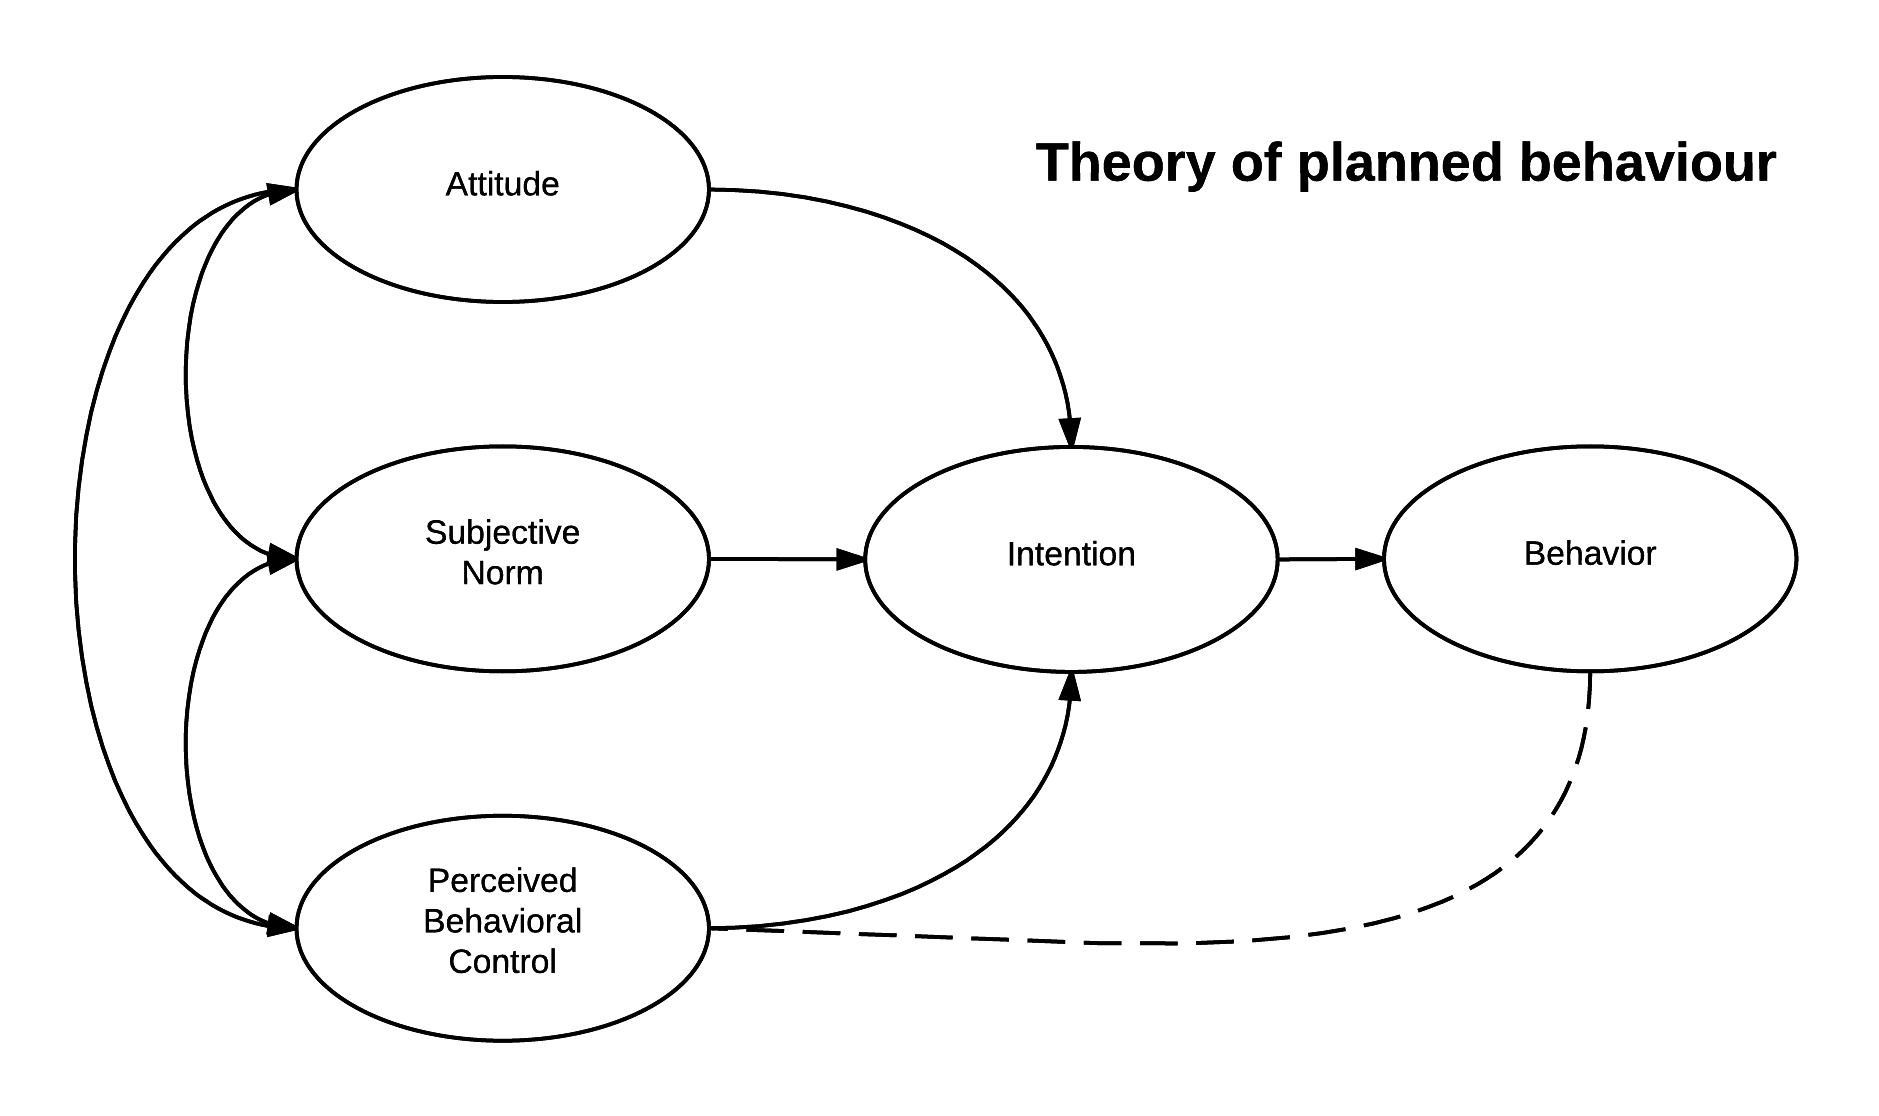
\includegraphics[width=0.8\textwidth]{Theory_of_planned_behavior_chart}}
%     \caption{ساختار نظریه رفتار برنامه ریزی شده
%       %\cite{kim2016integrated}
%     }
%     \label{fig:Theory_of_planned_behavior_chart}
%   \end{figure}\\

% \includepdf[pages={1}]{sexualityAgainstPopulation.pdf}
\begin{figure}[htpb]
    \centering
    \includegraphics[width=0.8\textwidth]{./img/sexualityAgainstPopulation.pdf}
    \caption{فراوانی جنسیت بیان شده در نمونه}
    \label{fig:sexualityAgainstPopulation}
\end{figure}
بعد از حذف داده‌های مربوط به آزمودنی‌هایی که اطلاعات مخدوش یا غیر قابل استفاده داشتند، تعداد
\CleanedSampleSize
باقی ماندند.

\subsection{نتایج آزمون جهت‌گیری ارزش اجتماعی}
از میان همه شرکت کنندگان
\noOfIndividualisticParticipants
نفر در دسته
\textit{
    \gls{Individualistic}
}
،
\noOfCompetitiveParticipants
نفر در دسته
\textit{
    \gls{Competitive}
}
،
\noOfCooperativeParticipants
نفر در دسته
همکاری‌کننده
و
\noOfAltruisticParticipants
نفر در دسته
دیگر‌خواه
قرار داشتند.
(
تصویر \label{fig:SVOAgainstPopulation}
)

تصویر \label{fig:sexualityAndSVOAgainstPopulation}

\begin{figure}[htpb]
    \centering
    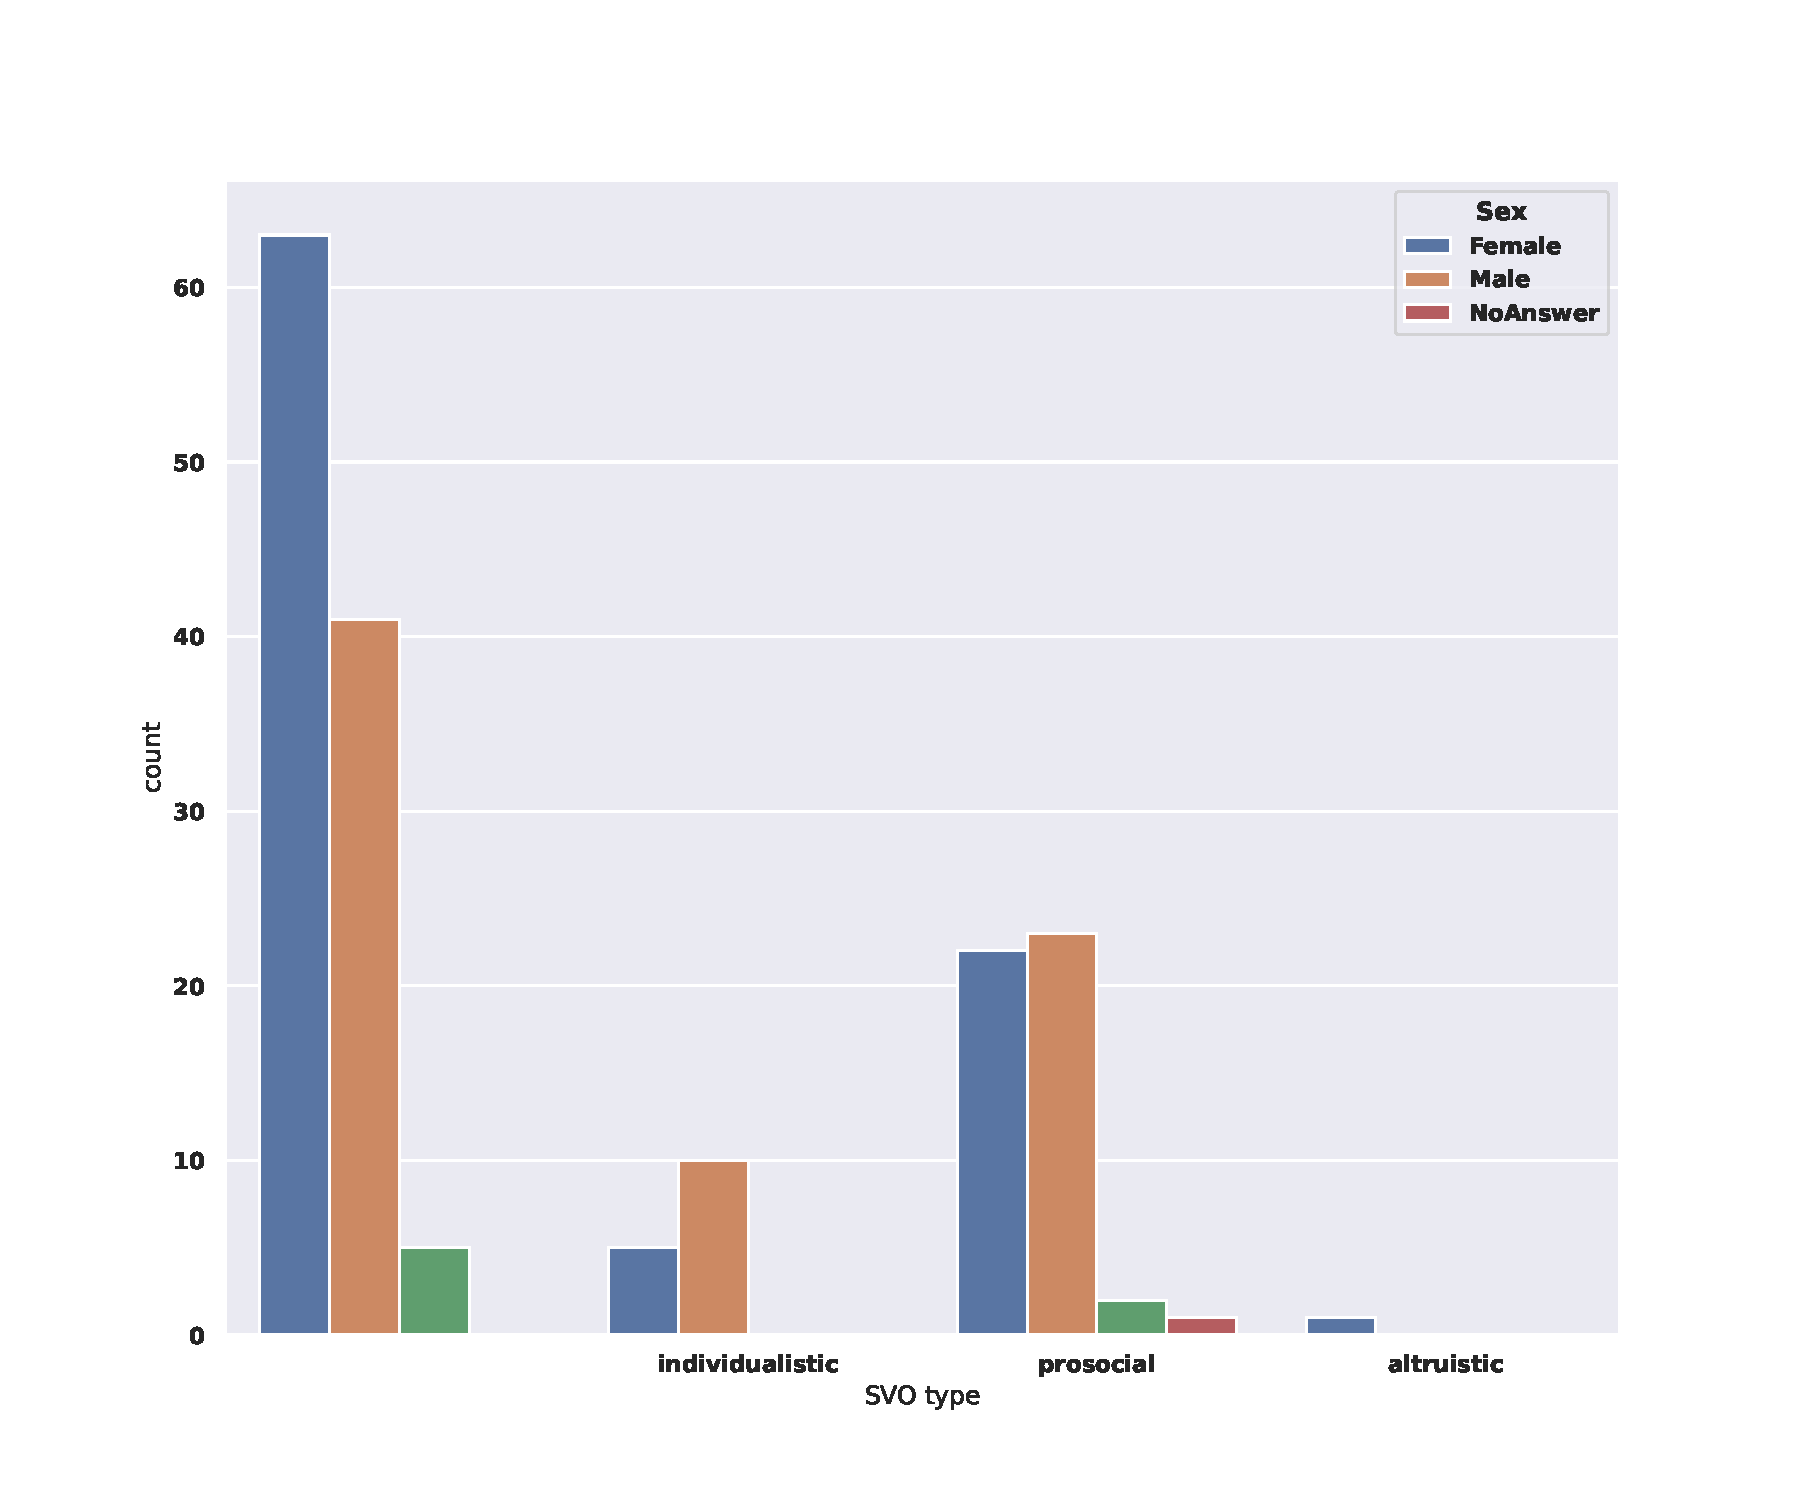
\includegraphics[width=0.8\textwidth]{./img/sexualityAndSVOAgainstPopulation.pdf}
    \caption{فراوانی دسته‌های رویکرد ارزش اجتمعای با توجه به جنسیت}
    \label{fig:sexualityAndSVOAgainstPopulation}
\end{figure}


\begin{figure}[htpb]
    \centering
    
\includegraphics[width=0.8\textwidth]{./img/SVOAgainstPopulation.pdf}
    \caption{فراوانی دسته‌های رویکرد ارزش اجتماعی}
    \label{fig:SVOAgainstPopulation}
\end{figure}
میانگین کلی نمره‌ای که همه آزمودنی‌ها در هر دو گروه به ۱۴ سوال هر دو دسته
نمرات از دید خود
\!(باور به ارزش اطلاعات)
\meanOfSelfWTPAllTwoParticipantGroupsAllTwoQuestionSection
با انحراف استاندارد
\SDOfSelfWTPAllTwoParticipantGroupsAllTwoQuestionSection
و از دید دیگران
\meanOfOtherWTPAllTwoParticipantGroupsAllTwoQuestionSection
\!(باور هنجاری به ارزش اطلاعات)
با انحراف استاندارد
\SDOfOtherWTPAllTwoParticipantGroupsAllTwoQuestionSection
بود.

\begin{figure}[htpb]
    \centering
    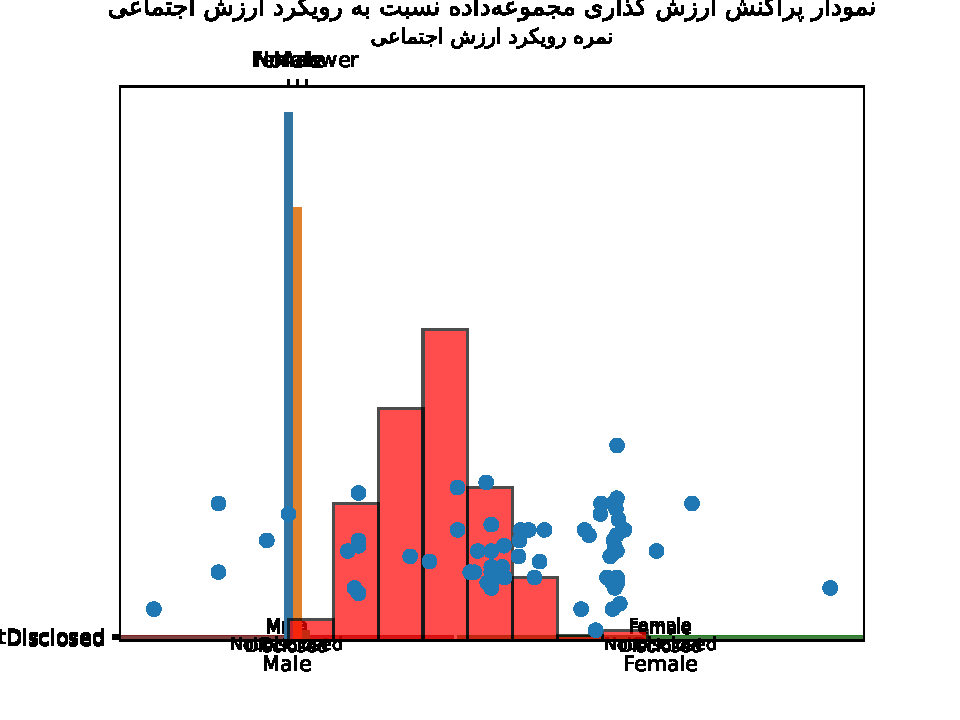
\includegraphics[width=0.8\textwidth]{./img/ScatterSVOScoreDarkTriadScore.pdf}
    \caption{نمودار پراکنش نمره رویکرد ارزش اجتماعی را نسبت به نمره سه‌گانه تاریک نشان می دهد. }
    \label{fig:ScatterSVOScoreDarkTriadScore}
\end{figure}
شکل 
\label{fig:sexualityAndSVOAgainstPopulation}
نمودار پراکنش نمره رویکرد ارزش اجتماعی را نسبت به نمره سه‌گانه تاریک نشان می دهد. 
و در شکل 
\label{fig:SexToDTR}
فراوانی نمره‌های پرسشنامه سه‌گانه تاریک مشخس شده است.




\begin{figure}[htpb]
    \centering
    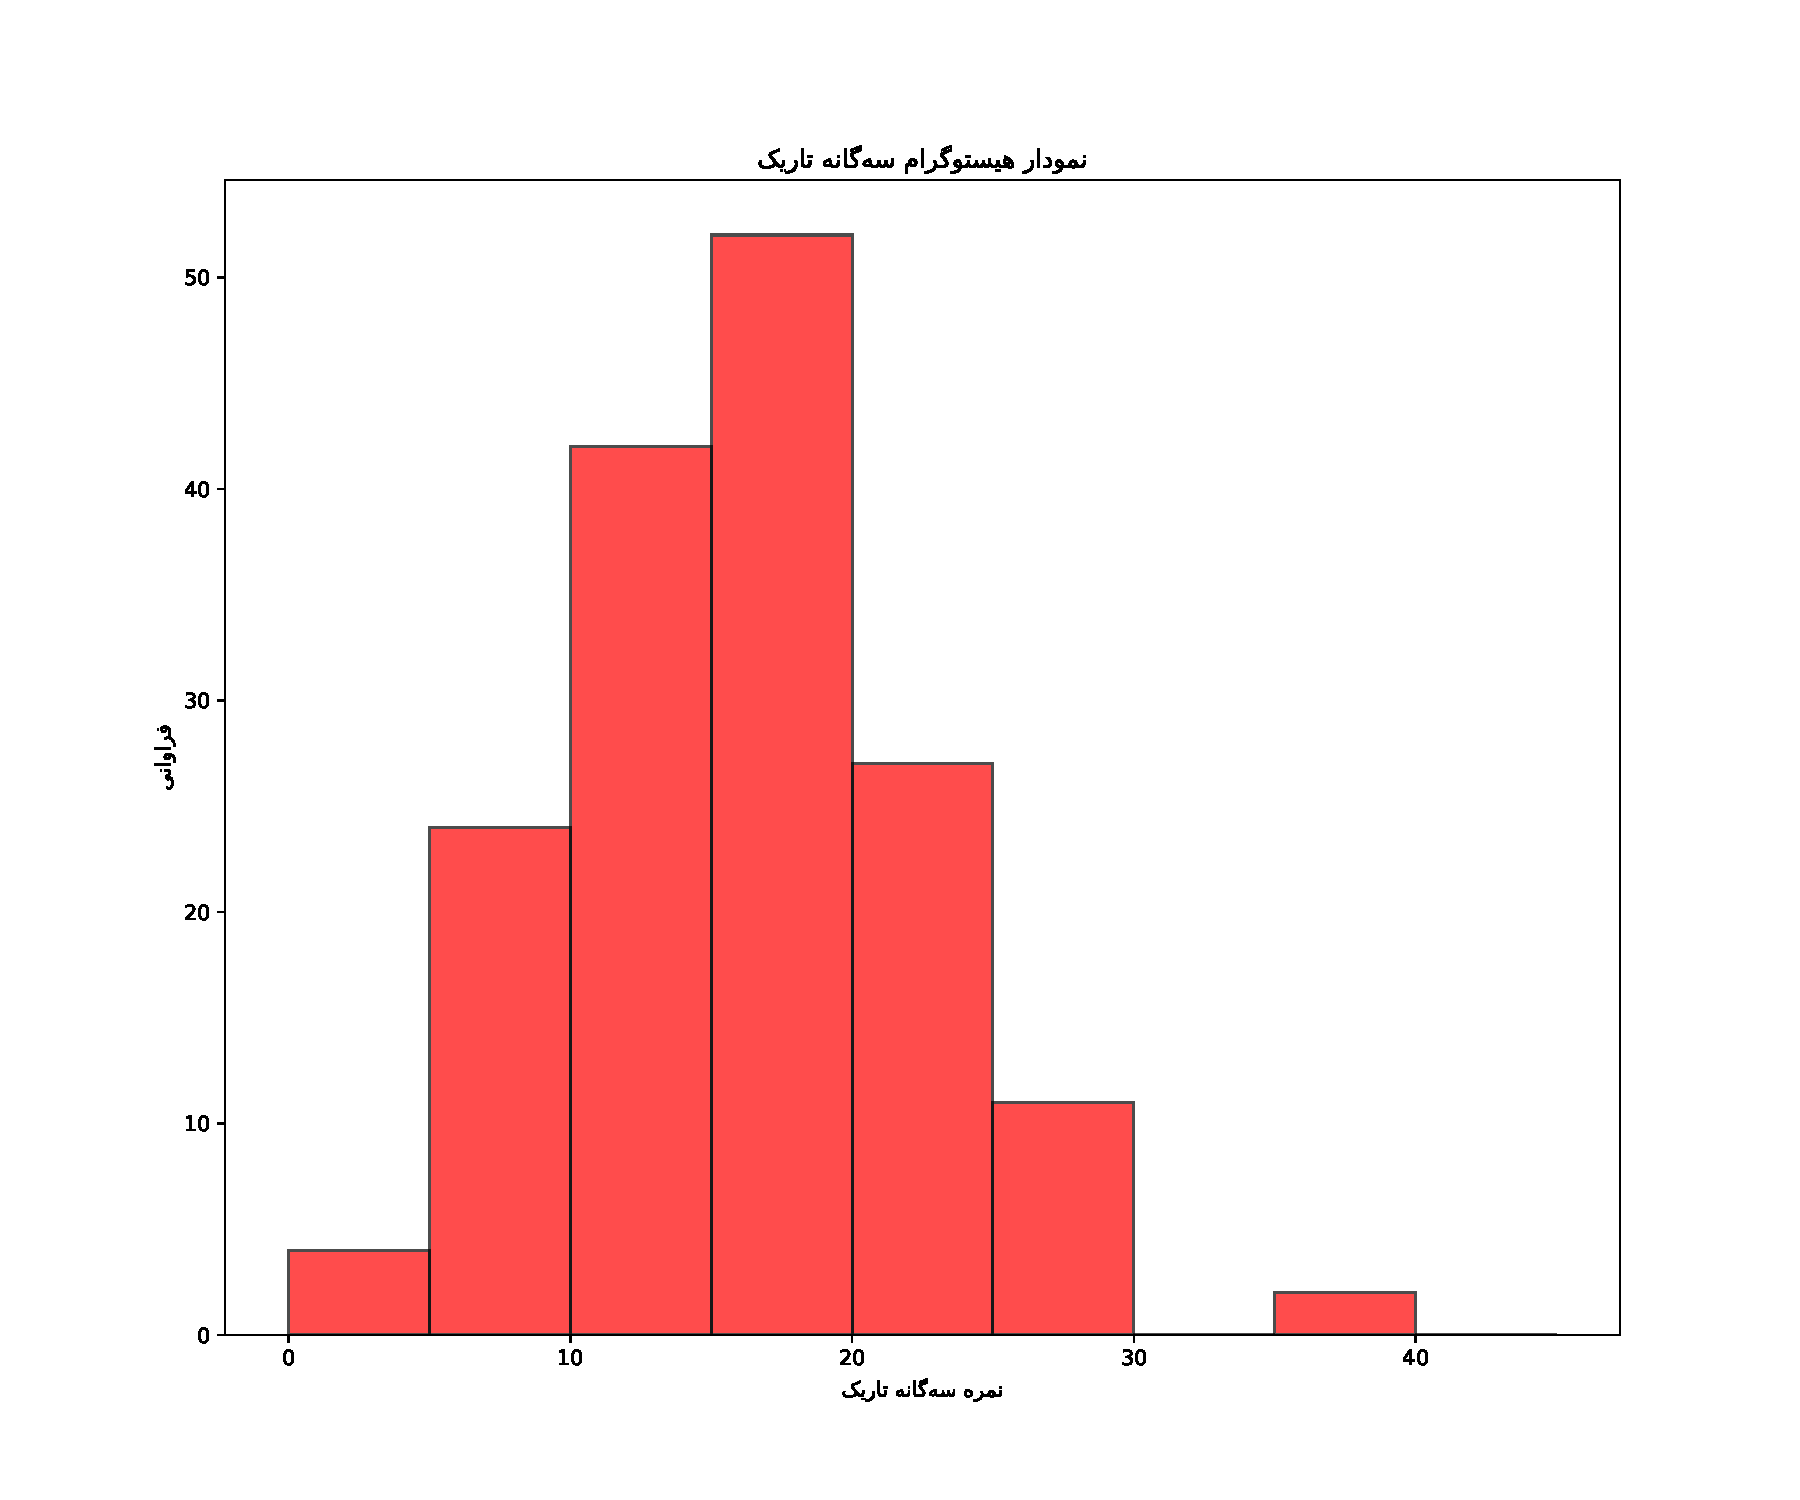
\includegraphics[width=0.8\textwidth]{./img/SexToDTR.pdf}
    \caption{نمودار پراکنش نمره رویکرد ارزش اجتماعی را نسبت به نمره سه‌گانه تاریک نشان می دهد. }
    \label{fig:SexToDTR}
\end{figure}


\begin{table}[h!]
    \begin{center}
      \caption{More columns.}
      \label{tab:table1}
      \begin{tabular}{l|c|r|l}
        \textbf{Value 1} & \textbf{Value 2} & \textbf{Value 3} & \textbf{Value 4}\\ % <-- added & and content for each column
        $\alpha$ & $\beta$ & $\gamma$ & $\delta$ \\ % <--
        \hline
        1 & 1110.1 & a & e\\ % <--
        2 & 10.1 & b & f\\ % <--
        3 & 23.113231 & c & g\\ % <--
      \end{tabular}
    \end{center}
  \end{table}
% \subsection{پایایی پرسشنامه سیاهه ارزش‌گذاری مجموعه‌داده}
% میان نمرات به نیمه اول این پرسشنامه برای اندازه گیری
% باور به ارزش اطلاعات
% \!(ارزش‌گذاری از دید خود)
% \meanOfSelfWTPAllTwoParticipantGroupFirstQuestionSection
% با انحراف معیار
% \SDOfSelfWTPAllTwoParticipantGroupsFirstQuestionSection
% و نیمه دوم
% \meanOfOtherWTPAllTwoParticipantGroupsSecondQuestionSection
% \SDOfOtherWTPAllTwoParticipantGroupsSecondQuestionSection
% بود. با توجه به وجود
% %  عدم وجود
% همبستگی میان این دو نیمه
% (
% $
%     r=
%     \PiersonrValueForCorrelationBetweenFirstAndSecondPartOfQuestionsForSelfValuation
%     ,
%     P=
%     \PvalueForCorrelationBetweenFirstAndSecondPartOfQuestionsForSelfValuation
% $
% )
% این آزمون برای اندازه گیری باور به ارزش اطلاعات از دید خود در گروه‌های هفت‌گانه دارای پایایی درونی با
% روش نیمه‌سازی پرسشنامه است.
% همچنین با توجه به وجود
% %  عدم وجود
% همبستگی میان این دو نیمه
% (
% $
%     \!r=
%     \!\PiersonRValueForCorrelationBetweenFirstAndSecondPartOfQuestionsforOtherValuation
%     \!,
%     P=
%     \!\PvalueForCorrelationBetweenFirstAndSecondPartOfQuestionsForOtherValuation
% $
% )
% این آزمون برای اندازه گیری باور به ارزش اطلاعات از دید دیگری در گروه‌های هفت‌گانه دارای پایایی درونی با
% روش
% \textit{
%     \gls{Split Half}
% }
% پرسشنامه است.


% میانگین نمرات آزمودنی ها به دسته اول سوالات
\section{اعتبارسنجی}
% از طریق مقایسهٔ نتایج با نتایج کارهای دیگران، استفاده از روش‌های تحلیل پایائی
% \lr{(reliability)}
% و اعتبار
% \lr{(validity)}،
% نظرگیری از خبرگان
% \lr{(expert judgment or feedback)}
% و یا
% \lr{triangulation}
% انجام می‌شود.
		% فصل چهارم: نتایج
% !TeX root=main.tex
\chapter{بحث و نتیجه‌گیری}
%\thispagestyle{empty} 
\section{مقدمه}
% ^ %%%%%%%%%%%%%%%%%%%%%%%%%%%%%%%%%%%%%%%%%%%%%%%%%%%%%%%%%%
% ^ %%%%%%%%%%%%%%%%%%%%%%%%%%%%%%%%%%%%%%%%%%%%%%%%%%%%%%%%%%
% ^ %%%%%%%%%%%%%%%%%%%%%%%%%%%%%%%%%%%%%%%%%%%%%%%%%%%%%%%%%%
\subsection{نتایج مربوط به سه‌گانه تاریک}
پژوهش‌های پیشین میان ویژگی‌های تاریک و رفتار
به اشتراک گذاری اطلاعات خصوصی دیگران به شکل
\textit{
    شایعه پراکنی
}
\LTRfootnote{
    Gossip
}
رابطه مستقیم مشاهده شده است
\!\cite{hartungBetterItsReputation2019}
\!.
همچنین نمرات سه‌گانه تاریک پیشگوی رفتار نابهنجار در سطح
\textit{
    اجتماعی-روانشناختی
}
\LTRfootnote{
    Psychosocial
}
می‌باشد
\!\cite{murisMalevolentSideHuman2017}
\!.
رفتار ضد اجتماعی قوی‌ترین رابطه را با رفتار نابهنجار اجتماعی-روانشناختی دارد
\lr{(r = .29)}
\!. خودشیفتگی
\lr{(r = .24)}
و ماکیاولیسم
\lr{(r = .13)}
در رتبه‌های بعدی قرار می‌گیرند
\!.
در پژوهش حاضر میان رفتار به اشتراک‌گذاری اطلاعات شخصی دیگران و سه‌گانه تاریک رابطه مشاهده شد.
متغیر در لاتک را چطور .وارد کنم.
% ^ %%%%%%%%%%%%%%%%%%%%%%%%%%%%%%%%%%%%%%%%%%%%%%%%%%%%%%%%%%
% ^ %%%%%%%%%%%%%%%%%%%%%%%%%%%%%%%%%%%%%%%%%%%%%%%%%%%%%%%%%%
% ^ %%%%%%%%%%%%%%%%%%%%%%%%%%%%%%%%%%%%%%%%%%%%%%%%%%%%%%%%%%
\subsection{
    نتایج مربوط به
    \lr{SVO}
}
% ^ %%%%%%%%%%%%%%%%%%%%%%%%%%%%%%%%%%%%%%%%%%%%%%%%%%%%%%%%%%
% ^ %%%%%%%%%%%%%%%%%%%%%%%%%%%%%%%%%%%%%%%%%%%%%%%%%%%%%%%%%%
% ^ %%%%%%%%%%%%%%%%%%%%%%%%%%%%%%%%%%%%%%%%%%%%%%%%%%%%%%%%%%
\subsection{
    نتایج مربوط به کیفیت زندگی
}
در پژوهش‌های قبلی میان عامل خود‌افشاگری و
دامنه‌های کیفیت ارتباطات اجتماعی و کیفیت محیطی و
نمره کل کیفت زندگی در پرسشنامه کیفیت زندگی روابطی مشاهده شده است
\!\cite{chandraRelationshipPsychologicalMorbidity2003}
\!.
% تاکنون شما در پایان‌نامه‌ای که مشغول نوشتن آن هستید، پاسخ چهار سؤال را داده‌اید:
% \begin{itemize}
% 	\item
% 	چرا تحقیق را انجام دادید؟ (مقدمه)
% 	\item
% 	دیگران در این زمینه‌ چه کارهایی کرده‌اند و تمایز کار شما با آنها؟ (مرور ادبیات)
% 	\item
% 	چگونه تحقیق را انجام دادید؟ (روش‌ها)
% 	\item
% 	چه از تحقیق به دست آوردید؟ (یافته‌ها)
% \end{itemize}
% حال زمان آن فرا رسیده که با توجه به تمامی مطالب ذکر شده، در نهایت به سؤال آخر پاسخ دهید:
% \begin{itemize}
% 	\item
% 	چه برداشتی از یافته‌های تحقیق کردید؟ (نتیجه‌گیری)
% \end{itemize}
% در واقع در این بخش، هدف، پاسخ به این سوال است که چه برداشتی از یافته‌ها کردید و این یافته‌ها چه فایده‌ای دارند؟

% نتیجه‌گیری مختصری بنویسید. ارائهٔ داده‌ها، نتایج و یافته‌ها در فصل چهارم ارائه می‌شود. در این فصل تفاوت، تضاد یا تطابق بین نتایج تحقیق با نتایج دیگر محققان باید ذکر شود.
% \emph{تفسیر و تحلیل نتایج نباید بر اساس حدس و گمان باشد}،
% بلکه باید
% \textbf{برمبنای نتایج عملی استخراج‌شده}
% از تحقیق و یا
% \textbf{استناد به تحقیقات دیگران}
% باشد.
% با توجه به حجم و ماهیت تحقیق و با صلاحدید استاد راهنما، این فصل می‌تواند تحت عنوانی دیگر بیاید یا به دو فصل جداگانه با عناوین مناسب، تفکیک شود. اين فصل فقط باید به جمع‌بندی دست‌آوردهای فصل‌های سوم و چهارم محدود و از ذکر موارد جدید در آن خودداری شود. در عنوان این فصل، به جای کلمهٔ «تفسیر» می‌توان از واژگان «بحث» و «تحلیل» هم استفاده کرد. این فصل شاید مهم‌ترین فصل پایان‌نامه باشد.

% در این فصل خلاصه‌ای از یافته‌های تحقیق جاری ارائه می‌شود. این فصل می‌تواند حاوی یک مقدمه، شامل مروری اجمالی بر مراحل انجام تحقیق باشد (حدود یک صفحه). مطالب پاراگراف‌بندی شود و هر پاراگراف به یک موضوع مستقل اختصاص یابد. فقط به ارائهٔ یافته‌ها و دست‌آوردها بسنده شود و
% \emph{از تعمیم بی‌مورد نتایج خودداری شود.}
% تا حد امکان از ارائهٔ 
% \emph{جداول و نمودارها در این فصل اجتناب شود.}
% از ارائهٔ 
% \emph{عناوین کلی}
% در حوزهٔ تحقیق و قسمت پیشنهاد پیشنهاد تحقیقات آتی خودداری شود و کاملاً در چارچوب و زمينهٔ مربوط به تحقیق جاری باشد. این فصل حدود ۱۰-۱۵ صفحه است.

\section{محتوا}
% به ترتیب شامل موارد زیر است:

\subsection{جمع‌بندی}
% خلاصه‌ای از تمام یافته‌ها و دست‌آوردهای تحقیق جاری است.

\subsection{نوآوری}
% این قسمت، نوآوری تحقیق را بر اساس یافته‌های آن تشریح می‌کند. که دارای دو بخش اصلی است:
% \begin{enumerate}
% 	\item
% 	نوآوری تئوری، یعنی تمایز تئوریک کار با کارهای محققین قبلی.
% 	\item
% 	نوآوری عملی، یعنی توصیه‌های محقق به صنعت برای بهبود بخشیدن به کارها، بر اساس یافته‌های تحقیق.
% \end{enumerate}

\subsection{پیشنهادها}
 با  توجه به اینکه  حریم خصوصی افراد یکی از متغیر‌های اصلی در زمان جمع آوری داده بود، رفتار‌های متنوعی در آزمودنی‌ها حین انجام آزمایش به وجود آمد. رها کردن انجام آزمایش یکی از این رفتار‌ها بود. بررسی این رفتار به عنوان یک متغیر، می‌تواند مهم تلقی شود.
% این بخش، عناوین و موضوعات پیشنهادی را برای تحقیقات آتی،
% \emph{بیشتر در زمينهٔ مورد بحث در آينده}
% ارائه می‌کند.

\subsection{محدودیت‌ها}
یک محدودیت اساسی  که سبب‌ساز ضرورت اجرا کردن آزمایش به صورت پایلوت در دفعات متعدد شد، عدم دسترسی به آزمودنی‌ها بود. معمولا در چنین پژوهش‌های میدانی که توسط آزمون‌های مبتنی بر وب انجام می‌گیرد از سرویس آمازون مکانیکال تورک و یا سرویس های مشابه مانند 
\textit{
    \gls{Prolific}
}
استفاده می‌شود. این سرویس‌ها امکان استفاده از آزمودنی‌ها با شرایط قابل قبول از نظر سوابق قبلی آن‌ها، را امکان‌پذیر می‌سازند. در این پژوهش از شبکه‌هایی اجتماعی مانند اینستاگرام، تلگرام، توییتر و واتساپ برای جذب آزمودنی‌ها استفاده شد. در نتیجه غربالگری افراد بر اساس شرایط قابل تایید 
\textit{
    \gls{Exclusion criteria}
}
وجود نداشت.
\subsection{محدودیت‌های ابزار سنجش نگرش به انواع اطلاعات خصوصی}
در این پژوهش از برای سنجش 
{\textit{\gls{Attitude}}}
نسب به ارزش انواع داده های خصوصی از دید کاربران 
(ضمیمه \ref{app:questionnaires})
استفاده شده است.
		% فصل پنجم: بحث و نتیجه‌گیری

% مراجع
% اگر از استیل‌های natbib استفاده می‌کنید باید دو خط را در فایل commands.tex تغییر دهید.
\pagestyle{empty}
{
    \onehalfspacing
    % \bibliographystyle{plain-fa} % or plainnat-fa for author-date
    \bibliographystyle{plainnat-fa} % or plainnat-fa for author-date
    % \bibliography{./tex/MyReferences}
    \bibliography{./tex/MyLibrary}



}

\pagestyle{fancy}

\appendix
% فصلهای پس از این قسمت به عنوان ضمیمه خواهند آمد.
% چندخط اول فایل appendix1 باید در فایل اولین پیوست بیاید.
% !TeX root=main.tex
%% دو سری دستور زیر باید در اولین فایل پیوست باشند. آنها را حذف نکنید!
% دستورات لازم برای تبدیل «فصل آ» به «پیوست آ» در فهرست مطالب
\addtocontents{toc}{
    \protect\renewcommand\protect\cftchappresnum{\appendixname~}%
    \protect\setlength{\cftchapnumwidth}{\mylenapp}}
    
\let\Chapter\chapter
% دستورات لازم برای شماره‌گذاری صفحات پیوست‌ها بشکل آ-۱ (فعلا با glossaries سازگار نیست)
% \pretocmd{\chapter}{
%  \clearpage
%  \pagenumbering{arabic}
%  \renewcommand*{\thepage}{\rl{\thechapter-\arabic{page}}}}{}{}
%%%%%%%%%%%%%%%%%%%%%%%%%%%%%%%%%%%%%
    
\chapter{پرسشنامه‌ها}
\label{app:questionnaires}
پرسشنامه ۱
% 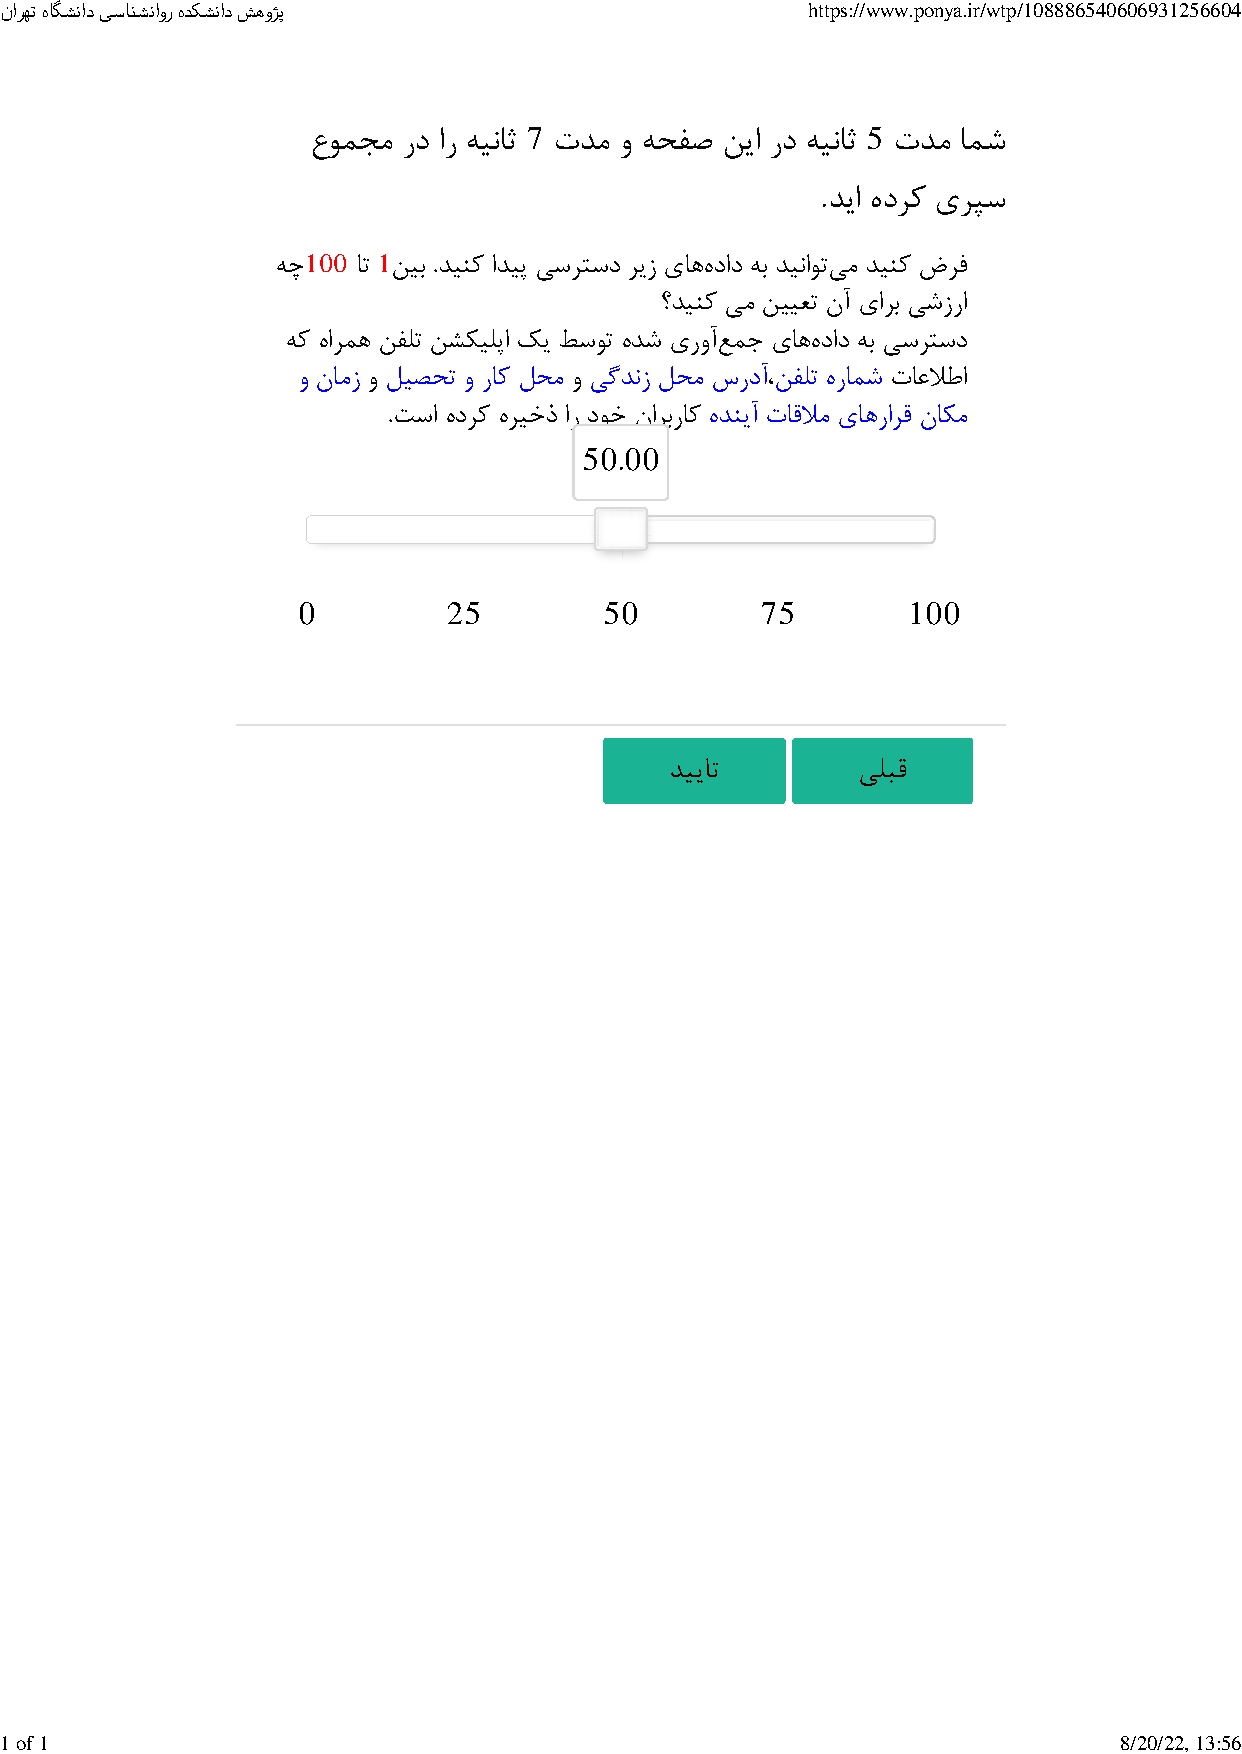
\includepdf[pages={1-3,{},8,10-12}]{questionnares/wtp.pdf}
% 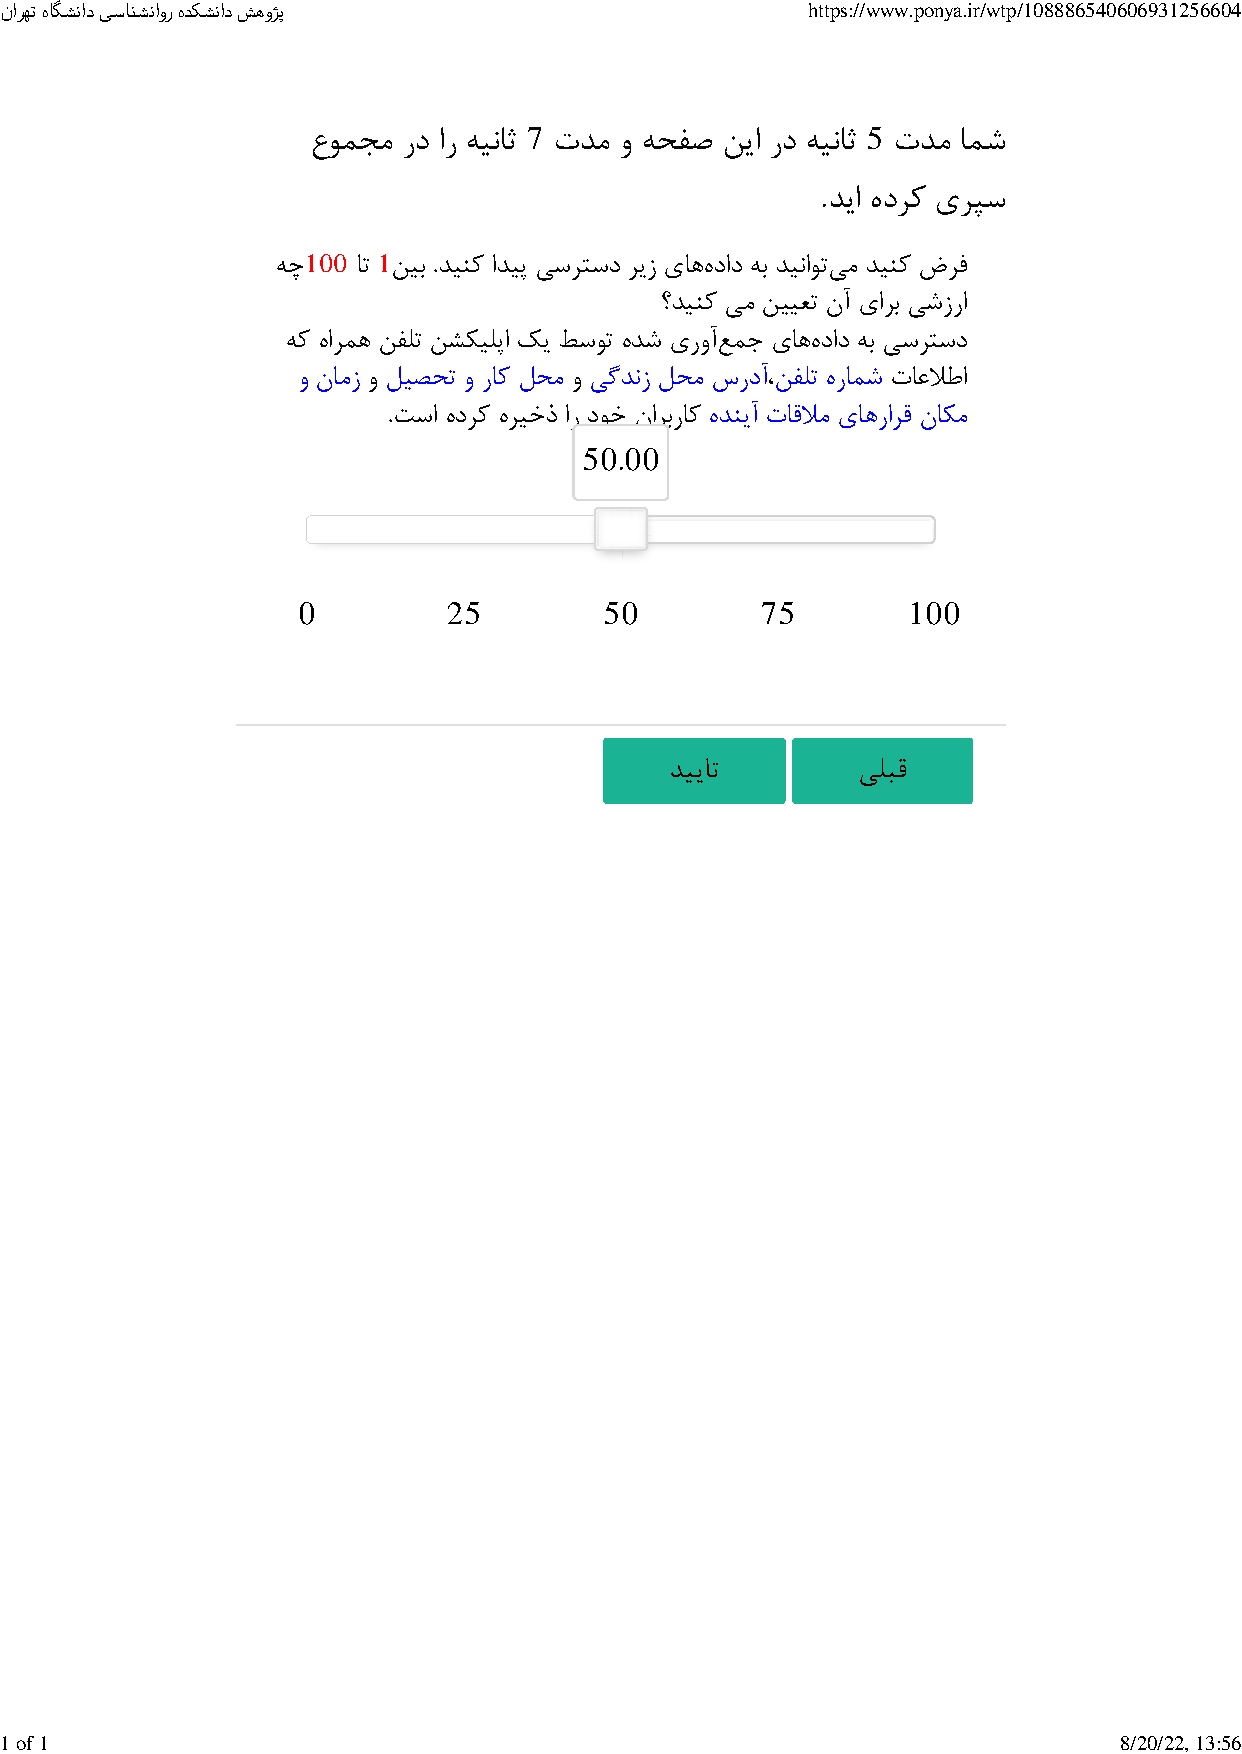
\includepdf[pages={1}]{./questionnares/wtp.pdf}
\begin{figure}[htpb]
    \centering
    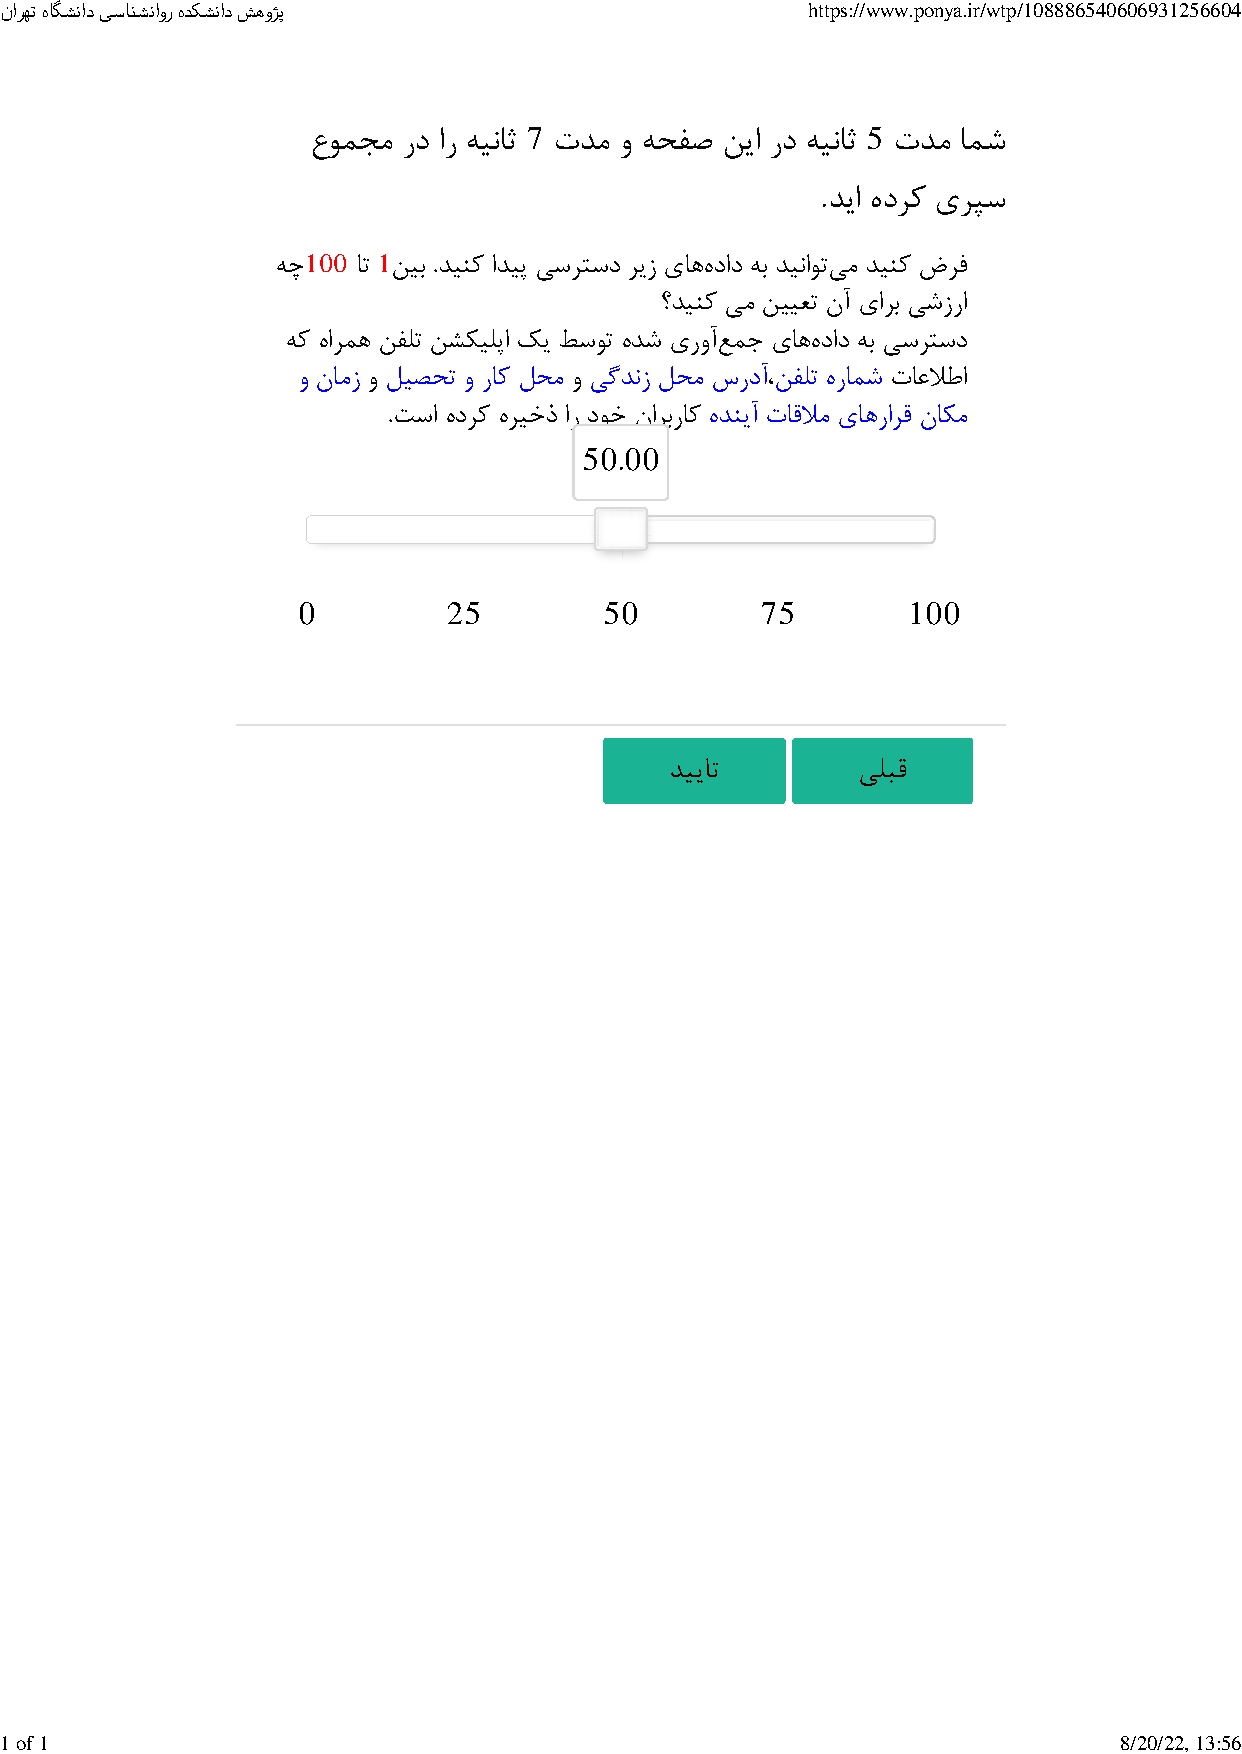
\includegraphics[width=0.8\textwidth]{./questionnares/wtp.pdf}
    \caption{The first page of the \texttt{tikz} reference manual.}
    \label{fig:tikzpgf}
\end{figure}
پرسشنامه ۲

% %\thispagestyle{empty}
% در این فصل ویژگی‌های مهم و پرکاربرد زی‌پرشین و لاتک معرفی می‌شود. برای راهنمایی بیشتر و به‌کاربردن ویژگی‌های پیشرفته‌تر به راهنمای زی‌پرشین و راهنمای لاتک مراجعه کنید. برای آگاهی از دستورات لاتک که این خروجی را تولید کرده‌اند فایل \lr{appendix1.tex} را ملاحظه فرمایید.
% \footnote{بیشتر مطالب این بخش از مثال 
% \lr{xepersian\_example.tex}
% گرفته شده‌اند که توسط آقای امیرمسعود پورموسی آماده شده است.}

% \section{بندها و زیرنویس‌ها}
% هر جایی از نوشتهٔ خود، اگر می‌خواهید به سر سطر بروید و یک بند (پاراگراف) تازه را آغاز کنید، باید یک خط را خالی بگذارید%
% \footnote{یعنی دوبار باید کلید \lr{Enter} را بزنید.}
%  مانند این:

% حالا که یک بند تازه آغاز شده است، یک زیرنویس انگلیسی%
% \LTRfootnote{English Footnote!}
%  هم می‌نویسیم!
% \section{فرمول‌های ریاضی}
% \label{formula}

% اینجا هم یک فرمول می‌آوریم که شماره دارد:
% \begin{equation}\label{eq:yek}
% A=\frac{c}{d}+\frac{q^2}{\sin(\omega t)+\Omega_{12}}
% \end{equation}
% در لاتک می‌توان به کمک فرمان 
% \lr{\textbackslash label\{\}}
% به هر فرمول یک نام نسبت داد. در فرمول بالا نام \lr{eq:yek} را برایش گذاشته‌ایم (پروندهٔ \lr{tex} همراه با این مثال را ببینید). این نام ما را قادر می‌کند که بعداً بتوانیم با فرمان
% \lr{\textbackslash ref\{eq:yek\}}
% به آن فرمول با شماره ارجاع دهیم. یعنی بنویسیم فرمول \ref{eq:yek}. 
% لاتک خودش شمارهٔ این فرمول‌ها را مدیریت می‌کند.\footnote{یعنی اگر بعداً فرمولی قبل از این فرمول بنویسیم، خودبه‌خود شمارهٔ این فرمول و شمارهٔ ارجاع‌ها به این فرمول یکی زیاد می‌شود. دیگر نگران شماره‌گذاری فرمول‌های خود نباشید!} این هم یک فرمول که شماره ندارد:
% $$A=|\vec{a}\times \vec{b}| + \sum_{n=0}^\infty C_{ij}$$

% این هم عبارتی ریاضی مانند 
% $\sqrt{a^2+b^2}$
%  که بین متن می‌آید.
% \subsection{یک زیربخش}
% \label{zirbakhsh}

% این زیربخش \ref{zirbakhsh} است؛ یعنی یک بخش درون بخش \ref{formula} است.
% \subsubsection{یک زیرزیربخش}
% این هم یک زیرزیربخش است. در لاتک می‌توانید بخش‌های تودرتو در نوشته‌تان تعریف کنید تا ساختار منطقی نوشته را به خوبی نشان دهید. می‌توانید به این بخش‌ها هم با شماره ارجاع دهید، مثلاً بخش فرمول‌های ریاضی شماره‌اش \ref{formula} است.
% \section{نوشته‌های فارسی و انگلیسی مخلوط}
% نوشتن یک کلمهٔ انگلیسی بین متن فارسی بدیهی است، مانند Example در این جمله.
% نوشتن یک عبارت چندکلمه‌ای مانند
%  \lr{More than one word} کمی پیچیده‌تر است.

% اگر ناگهان تصمیم بگیرید که یک بند کاملاً انگلیسی را بنویسید، باید:
% \begin{latin}
% This is an English paragraph from left to right. You can write as much as you want in it.
% \end{latin}
% \section{افزودن تصویر به نوشته}
% پروندهٔ تصویر دلخواه خود را در کنار پروندهٔ \lr{tex} قرار دهید. سپس به روش زیر تصویر را در نوشتهٔ خود بیاورید:
% \begin{latin}
% \begin{verbatim}
% \includegraphics{YourImageFileName}
% \end{verbatim}
% \end{latin}
% به تصویرها هم مانند فرمول‌ها و بخش‌ها می‌توان با شماره ارجاع داد. مثلاً تصویر \ref{fig:shir} یک شیر علاقه‌مند به لاتک را در حال دویدن نشان می‌دهد. برای جزئیات بیشتر دربارهٔ روش گذاشتن تصویرها در نوشته باید راهنماهای لاتک را بخوانید.
% \begin{figure}[ht]
% \centerline{
\includegraphics[width=5cm]{lion}}
% \caption{در این تصویر یک شیر علاقه‌مند به لاتک را در حال دویدن می‌بینید.}
% \label{fig:shir}
% \end{figure}

% به تصویرها هم مانند فرمول‌ها و بخش‌ها می‌توان با شماره ارجاع داد. مثلاً تصویر بالا شماره‌اش \ref{fig:shir} است. برای جزئیات بیشتر دربارهٔ روش گذاشتن تصویرها در نوشته باید راهنماهای لاتک را بخوانید.

% \section{محیط‌های شمارش و نکات}
% برای فهرست‌کردن چندمورد، اگر ترتیب برایمان مهم نباشد:
% \begin{itemize}
% \item مورد یکم
% \item مورد دوم
% \item مورد سوم
% \end{itemize}
% و اگر ترتیب برایمان مهم باشد:
    % \begin{enumerate}
    % \item مورد یکم
    % \item مورد دوم
    % \item مورد سوم
    % \end{enumerate}
% می‌توان موردهای تودرتو داشت:
% \begin{enumerate}
% \item مورد ۱
% \item مورد ۲
% \begin{enumerate}
% \item مورد ۱ از ۲
% \item مورد ۲ از ۲
% \item مورد ۳ از ۲
% \end{enumerate}
% \item مورد ۳
% \end{enumerate}
% شماره‌گذاری این موردها را هم لاتک انجام می‌دهد.

% \section{تعریف و قضیه}
% برای ذکر تعریف، قضیه و مثال مثالهای ذیل را ببینید.
% \begin{definition}
% مجموعه همه ارزیابی‌های  (پیوسته)  روی $(X,\tau)$، دامنه توانی احتمالی
% \index{دامنه توانی احتمالی}
% $ X $
% نامیده می‌شود.
% \end{definition}
% \begin{theorem}[باناخ-آلااغلو]
% \index{قضیه باناخ-آلااغلو}
% اگر $ V $ یک همسایگی $ 0 $ در فضای برداری 
% \index{فضای!برداری}
%  توپولوژیکی $ X $ باشد و 
% \begin{equation}\label{eq1}
% K=\left\lbrace \Lambda \in X^{*}:|\Lambda x|\leqslant 1 ; \ \forall x\in V\right\rbrace,
% \end{equation}
% آنگاه $ K $،  ضعیف*-فشرده است که در آن، $ X^{*} $ دوگان
% \index{فضای!دوگان}
%  فضای برداری توپولوژیکی $ X $ است به ‌طوری که عناصر آن،  تابعی‌های 
% خطی پیوسته
% \index{تابعی خطی پیوسته}
%  روی $X$ هستند.
% \end{theorem}
% تساوی \eqref{eq1} یکی از مهم‌ترین تساوی‌ها در آنالیز تابعی است که در ادامه، به وفور از آن استفاده می‌شود.
% \begin{example}
% برای هر فضای مرتب، گردایه 
% $$U:=\left\lbrace U\in O: U=\uparrow U\right\rbrace $$
% از مجموعه‌های بالایی باز، یک توپولوژی تعریف می‌کند که از توپولوژی اصلی، درشت‌تر  است.
% \end{example}
% حال تساوی 
% \begin{equation}\label{eq2}
% \sum_{n=1}^{+\infty} 3^{n}x+7x=\int_{1}^{n}8nx+\exp{(2nx)}
% \end{equation}
% را در نظر بگیرید. با مقایسه تساوی \eqref{eq2} با تساوی \eqref{eq1} می‌توان نتیجه گرفت که ...


% \section{چگونگی نوشتن و ارجاع به مراجع}
% \label{Sec:Ref}


% در لاتک به راحتی می‌توان مراجع خود را نوشت و به آنها ارجاع داد. به عنوان مثال برای معرفی کتاب گنزالس \cite{Gonzalez02book} به عنوان یک مرجع می‌توان آنرا به صورت زیر معرفی نمود:

% \singlespacing
% \begin{LTR}
% \begin{verbatim}
% \bibitem{Gonzalez02book}
% Gonzalez, R.C., and Woods, R.E. {\em Digital Image Processing}, 3rd ed..
% Prentice-Hall, Inc., Upper Saddle River, NJ, USA, 2006.
% \end{verbatim}
% \end{LTR}
% \doublespacing

% در دستورات فوق \lr{Gonzalez02book}  برچسبی است که به این مرجع داده شده است و با استفاده از دستور 
% \verb!\cite{Gonzalez02book}!
% می‌توان به آن ارجاع داد؛ بدون این که شماره‌اش را در فهرست مراجع‌مان بدانیم.

% اگر این اولین مرجع ما باشد در قسمت مراجع به صورت زیر خواهد آمد:\\
% 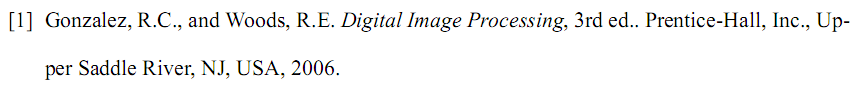
\includegraphics[width=\textwidth]{gonzalez.png}

% این شیوهٔ تعریف مراجع بسیار ابتدایی است و اگر فرمت مراجع، ترتیب یا تعداد آنها را خواسته باشید تغییر دهید، به عنوان مثال ابتدا حرف اول نام نویسنده بیاید و سپس نام خانوادگی، باید همه کارها را به صورت دستی انجام دهید!
% چون در یک \پ یا مقاله باید کنترل کاملی بر مراجع خود داشته باشید و به راحتی بتوانید قالب مراجع را عوض کنید، بنابراین می‌بایست از \lr{Bib\TeX} استفاده کنید که درپیوست  \ref{app:refMan} به  آن پرداخته خواهد شد.
		% پیوست اول: آشنایی مقدماتی با لاتک
% !TeX root=main.tex

% \chapter{‌جدول، نمودار و الگوریتم در لاتک}
% \label{app:latex:more}
%\thispagestyle{empty}

% در این بخش نمونه مثالهایی از جدول، شکل، نمودار، الگوریتم و معادلات ریاضی را در لاتک خواهیم دید.
% دقت کنید که در پایان‌نامه‌ها و مقالات، باید قاعدهٔ «ارجاع به جلو%
% \LTRfootnote{Forward Referencing}»
% رعایت شود؛ یعنی ابتدا در متن به شمارهٔ شکل، جدول یا معادله اشاره شود و بعد از آن (زیر آن) خود شکل، جدول یا معادله رسم شود. (توضیحات بیشتر در قسمت
% \ref{sec:floatObjs}).

% \section{جدول}
% دستور اصلی برای رسم جدول در لاتک
% \verb|tabular|
% می‌باشد که جدول
% \eqref{tab:motionModels}
% با استفاده از آن کشیده شده است؛ در
% \verb|tabular|
% عرض جدول برابر با مجموع عرض ستون‌ها و حداکثر مساوی عرض متن است.
% \begin{table}[ht]
% 	\caption{مدلهای تبدیل.}
% 	\label{tab:motionModels}
% 	\centering
% 	\onehalfspacing
% 	\begin{tabular}{|r|c|l|r|}
% 		\hline نام مدل & درجه آزادی & تبدیل مختصات                & توضیح         \\
% 		\hline انتقالی & ۲          & $\begin{aligned} x'=x+t_x \\ y'=y+t_y \end{aligned}$ & انتقال دوبعدی \\
% 		\hline اقلیدسی & ۳          & $\begin{aligned} x'=x\cos\theta - y\sin\theta+t_x \\ y'=x\sin\theta+y\cos\theta+t_y \end{aligned}$ & انتقالی+دوران \\
% 		\hline
% 	\end{tabular}
% \end{table}

% برای اینکه عرض جدول قابل کنترل باشد، باید از دستورات
% \verb|tabularx|،
% \verb|tabulary| یا
% \verb|tabu|
% استفاده کرد که راهنمای آنها در اینترنت وجود دارد.
% مثلاً جدول
% \ref{tab:motionModelsCont}
% با
% \verb|tabularx|
% رسم شده که عرض جدول در آن ثابت بوده و ستون‌های از نوع
% \verb|X|
% عرض خالی جدول را پر می‌کنند.
% \begin{table}[ht]
% 	\caption{مدلهای تبدیل دیگر.}
% 	\label{tab:motionModelsCont}
% 	\centering
% 	\onehalfspacing
% 	\begin{tabularx}{\textwidth}{|r|c|l|X|}
% 		\hline نام مدل & درجه آزادی & تبدیل مختصات                & توضیح              \\
% 		\hline مشابهت  & ۴          & $\begin{aligned} x'=sx\cos\theta - sy\sin\theta+t_x \\ y'=sx\sin\theta+sy\cos\theta+t_y  \end{aligned}$ & اقلیدسی+تغییرمقیاس \\
% 		\hline آفین    & ۶          & $\begin{aligned} x'=a_{11}x+a_{12}y+t_x \\ y'=a_{21}x+a_{22}y+t_y \end{aligned}$ & مشابهت+اریب‌شدگی    \\
% 		\hline
% 	\end{tabularx}
% \end{table}

% \section{معادلات ریاضی و ماتریس‌ها}
% تقریباً هر آنچه دانشجویان برای نوشتن فرمول‌های ریاضی لازم دارند، در کتاب
% \lr{mathmode}
% آمده است. کافیست در خط فرمان، دستور زیر را وارد کنید:
% \begin{latin}
% 	\texttt{texdoc mathmode}
% \end{latin}
% متن زیر شامل انواعی از اشیاء ریاضی است که با ملاحظه کدش می‌توانید با دستورات آن آشنا شوید.\\
% شناخته‌شده‌ترین روش تخمین ماتریس هوموگرافی الگوریتم تبدیل خطی مستقیم (\lr{DLT\LTRfootnote{Direct Linear Transform}}) است.  فرض کنید چهار زوج نقطهٔ متناظر در دو تصویر در دست هستند،  $\mathbf{x}_i\leftrightarrow\mathbf{x}'_i$   و تبدیل با رابطهٔ
% $\mathbf{x}'_i = H\mathbf{x}_i$
% نشان داده می‌شود که در آن:
% \[\mathbf{x}'_i=(x'_i,y'_i,w'_i)^\top  \]
% و
% \[ H=\left[
% 		\begin{array}{ccc}
% 			h_1 & h_2 & h_3 \\
% 			h_4 & h_5 & h_6 \\
% 			h_7 & h_8 & h_9
% 		\end{array}
% 		\right]\]
% رابطه زیر را برای الگوریتم  \eqref{alg:DLT} لازم داریم.
% \begin{equation}
% 	\label{eq:DLT_Ah}
% 	\left[
% 		\begin{array}{ccc}
% 			0^\top                  & -w'_i\mathbf{x}_i^\top & y'_i\mathbf{x}_i^\top  \\
% 			w'_i\mathbf{x}_i        & 0^\top                 & -x'_i\mathbf{x}_i^\top \\
% 			- y'_i\mathbf{x}_i^\top & x'_i\mathbf{x}_i^\top  & 0^\top
% 		\end{array}
% 		\right]
% 	\left(
% 	\begin{array}{c}
% 			\mathbf{h}^1 \\
% 			\mathbf{h}^2 \\
% 			\mathbf{h}^3
% 		\end{array}
% 	\right)=0
% \end{equation}

% \section{الگوریتم با دستورات فارسی}
% با مفروضات فوق، الگوریتم \lr{DLT} به صورت نشان داده شده در الگوریتم \eqref{alg:DLT}  خواهد بود.
% \begin{algorithm}[ht]
% 	\onehalfspacing
% 	\caption{الگوریتم \lr{DLT} برای تخمین ماتریس هوموگرافی.} \label{alg:DLT}
% 	\begin{algorithmic}[1]
% 		\REQUIRE $n\geq4$ زوج نقطهٔ متناظر در دو تصویر
% 		${\mathbf{x}_i\leftrightarrow\mathbf{x}'_i}$،\\
% 		\ENSURE ماتریس هوموگرافی $H$ به نحوی‌که:
% 		$\mathbf{x}'_i = H \mathbf{x}_i$.
% 		\STATE برای هر زوج نقطهٔ متناظر
% 		$\mathbf{x}_i\leftrightarrow\mathbf{x}'_i$
% 		ماتریس $\mathbf{A}_i$ را با استفاده از رابطهٔ \ref{eq:DLT_Ah} محاسبه کنید.
% 		\STATE ماتریس‌های ۹ ستونی  $\mathbf{A}_i$ را در قالب یک ماتریس $\mathbf{A}$ ۹ ستونی ترکیب کنید.
% 		\STATE تجزیهٔ مقادیر منفرد \lr{(SVD)}  ماتریس $\mathbf{A}$ را بدست آورید. بردار واحد متناظر با کمترین مقدار منفرد جواب $\mathbf{h}$ خواهد بود.
% 		\STATE  ماتریس هوموگرافی $H$ با تغییر شکل $\mathbf{h}$ حاصل خواهد شد.
% 	\end{algorithmic}
% \end{algorithm}

% \section{الگوریتم با دستورات لاتین}
% الگوریتم \ref{alg:RANSAC} یک الگوریتم با دستورات لاتین است.

% \begin{algorithm}[ht]
% 	\onehalfspacing
% 	\caption{الگوریتم \lr{RANSAC} برای تخمین ماتریس هوموگرافی.} \label{alg:RANSAC}
% 	\begin{latin}
% 		\begin{algorithmic}[1]
% 			\REQUIRE $n\geq4$ putative correspondences, number of estimations, $N$, distance threshold $T_{dist}$.\\
% 			\ENSURE Set of inliers and Homography matrix $H$.
% 			\FOR{$k = 1$ to $N$}
% 			\STATE Randomly choose 4 correspondence,
% 			\STATE Check whether these points are colinear, if so, redo the above step
% 			\STATE Compute the homography $H_{curr}$ by DLT algorithm from the 4 points pairs,
% 			\STATE $\ldots$ % الگوریتم کامل نیست
% 			\ENDFOR
% 			\STATE Refinement: re-estimate H from all the inliers using the DLT algorithm.
% 		\end{algorithmic}
% 	\end{latin}
% \end{algorithm}

% \section{درج کد}
% درج کد به زبان‌های مختلف به سادگی امکان‌پذیر است. برنامه
% \ref{code:matlabEx}
% یک قطعه کد
% \lr{MATLAB}
% را نشان می‌دهد.
% \singlespacing
% \begin{figure}
% 	\begin{LTR}
% 		\lstinputlisting[language=MATLAB, caption={نمونه کد \lr{MATLAB}}, label={code:matlabEx}]{MatlabExample.m}
% 	\end{LTR}
% \end{figure}
% \doublespacing

% \section{تصویر}
% نمونهٔ یک تصویر را در فصل قبل دیدیم. دو تصویر شیر کنار هم را نیز در شکل
% \ref{fig:twoLion}
% مشاهده می‌کنید.
% \begin{figure}[ht]
% 	\centering
% 	\subfigure[شیر ۱]{ \label{fig:twolion:one}
% 		
\includegraphics[width=0.3\textwidth]{lion}}
% 	%\hspace{2mm}
% 	\subfigure[شیر ۲]{ \label{fig:twolion:two}
% 		
\includegraphics[width=0.3\textwidth]{lion}}
% 	\caption{دو شیر}
% 	\label{fig:twoLion} %% label for entire figure
% \end{figure}

% \section{نمودار}
% لاتک بسته‌هایی با قابلیت‌های زیاد برای رسم انواع مختلف نمودارها دارد. مانند بسته‌های \lr{Tikz} و  \lr{PSTricks}. توضیح اینها فراتر از این پیوست کوچک است.%
% \footnote{
% 	مثال‌هایی از بکارگیری بسته
% 	\lr{Tikz}
% 	را می‌توانید در
% 	\url{http://www.texample.net/tikz/examples/}
% 	ببینید. توصیه می‌شود دانشجویانی که قصد درج اشکالی مانند گراف را در سند خود دارند، مثالهایی از سایت مذکور را ملاحظه فرمایند.
% }
% یک نمودار رسم شده با بسته‌ی
% \lr{TikZ}
% در شکل
% \ref{fig:parabola}
% نشان داده شده است.
% \begin{figure}[t]
% 	\centering
% 	\begin{tikzpicture}[scale=2.5]
% 		\shade[top color=blue,bottom color=gray!50]
% 		(0,0) parabola (1.5,2.25) |- (0,0);
% 		\draw (1.05cm,2pt) node[above]
% 		{$\displaystyle\int_0^{3/2} \!\!x^2\mathrm{d}x$};

% 		\draw[style=help lines] (0,0) grid (3.9,3.9)
% 		[step=0.25cm]      (1,2) grid +(1,1);

% 		\draw[->] (-0.2,0) -- (4,0) node[right] {$x$};
% 		\draw[->] (0,-0.2) -- (0,4) node[above] {$f(x)$};

% 		\foreach \x/\xtext in {1/1, 1.5/1\frac{1}{2}, 2/2, 3/3}
% 		\draw[shift={(\x,0)}] (0pt,2pt) -- (0pt,-2pt) node[below] {$\xtext$};

% 		\foreach \y/\ytext in {1/1, 2/2, 2.25/2\frac{1}{4}, 3/3}
% 		\draw[shift={(0,\y)}] (2pt,0pt) -- (-2pt,0pt) node[left] {$\ytext$};

% 		\draw (-.5,.25) parabola bend (0,0) (2,4) node[below right] {$x^2$};
% 	\end{tikzpicture}
% 	\caption{یک نمودار زیبا با ارقام فارسی و قابلیت بزرگ‌نمایی بسیار، بدون از دست دادن کیفیت.}
% 	\label{fig:parabola}
% \end{figure}

% \section{نحوه قرارگیری اشیای شناور}
% \label{sec:floatObjs}
% % شکل‌ها، جداول و الگوریتم‌ها در لاتک اشیای شناور محسوب می‌شوند؛ یعنی خود لاتک تصمیم می‌گیرد آنها را در کجای صفحه ترسیم کند تا زیباتر باشد. اما می‌توان به لاتک توصیه کرد که آن را در قسمت خاصی از صفحه رسم کند. برای اینکه قاعدهٔ «ارجاع به جلو» رعایت شود باید فقط از پرچم
% \verb|[ht]|
% استفاده کرد، که می‌گوید اگر جا شد شکل را دقیقاً در همین مکان و در غیراینصورت در بالای صفحه بعد رسم کن.
% % بنابراین دستورات درج تصویر، جدول و الگوریتم به صورت زیر باید باشند:

% \begin{latin}
% 	\begin{verbatim}
% 	\begin{figure/table/algorithm}[ht]
% 		...
% 	\end{figure/table/algorithm}
% \end{verbatim}
% \end{latin}		% پیوست دوم: جدول، نمودار و الگوریتم در لاتک
% !TeX root=main.tex
% \chapter{مراجع، واژه‌نامه و حاشیه‌نویسی}
% \label{app:refMan}
% %\thispagestyle{empty}

% \section{مراجع و نقل‌قول‌ها}
% \label{sec:refUsage}
% منابعِ پایان‌نامه، پایه و اساس تحقیق شما به حساب می‌آیند و ضرورت انجام مطالعه و روش‌های به کار رفته در بسیاری از قسمت‌های آن، به کمک منابع صورت می‌گیرد. در استفاده از مراجع علمی در پایان‌نامه، باید سعی کنید بیشتر از
% \textbf{منابع چاپ‌شده و مهم}
% استفاده کنید و
% \emph{ارجاع به داده‌های چاپ نشده، خلاصه‌ها و پایان‌نامه‌ها، سبب به‌هم‌خوردگی و کاهش اعتبار قسمت ارجاع منابع می‌شود.}
% استفاده از منابع و نقل قول‌هایی به تحقیق شما ارزش می‌دهند که
% \textbf{در راستای هدف تحقیق بوده و به آن اعتبار ببخشند.}
% برخی از دانش‌جویان تصوّر می‌کنند که کثرت نقل‌قول‌ها و ارجاعات زیاد، مهم‌ترین معیار علمی شدن پایان‌نامه است؛ حال آنکه استناد به تعداد کثیری از منابع بدون مطالعه دقیق آنها و استفادهٔ مستقیم در پایان‌نامه، می‌تواند نشان‌دهندهٔ عدم احساس امنیت نویسنده باشد!

% دو روش برای استفاده از نتایج، جملات، داده‌ها و روش‌های دیگران وجود دارد. یکی نقل‌قول مستقیم و دقیق است و دیگری استفاده غیرمستقیم در متن مقاله، که در ادامه به قواعد این دو نوع نقل‌قول و ارجاع‌دهی اشاره می‌کنیم:
% \begin{description}
% 	\item[نقل‌قول مستقیم:]
% 	نقل‌قول مستقیم باید دقیق و بدون هیچ تغییری در جملات باشد. بهتر است این‌گونه نقل‌قول‌ها تا حد امکان کوتاه باشد. جملات کوتاه داخل گیومه قرار می‌گیرند و باید به منبع دقیق آن، طبق روش ارجاع‌دهی به منابع، اشاره شود. به عنوان مثال در
% 	\cite{persianbib87userguide}
% 	آمده است که:
% 	\begin{quote}
% 		«با استفاده از فیلد
% 		\lr{AUTHORFA}
% 		می‌توان معادل فارسی نام نویسندگان مقالات لاتین را در متن داشت. معمولاً در اسناد فارسی خواسته می‌شود که پس از ذکر معادل فارسی نام نویسنده، نام لاتین نویسنده(ها) به عنوان پاورقی درج شود
% 		\citep{persianbib87userguide}.»
% 	\end{quote}
% 	\item[نقل‌قول غیرمستقیم:]
% 	نقل‌قول غیرمستقیم به معنی استفاده از ایده‌ها، نتایج، روش‌ها و داده‌های دیگران در درون متنِ پایان‌نامه، ولی به سبک خودتان و متناسب و هماهنگ با روند پایان‌نامهٔ شماست. در این حالت نیز باید متناسب با شیوهٔ ارجاع‌دهی به آن استناد شود.
% \end{description}

% با توجه به وجود سبک‌های مختلف ارجاع‌دهی، باید
% \textbf{روش قابل قبول و یکسانی}
% در طول پایان‌نامه برای اشاره به مراجع در متن و همچنین تهیه فهرست مراجع در انتهای پایان‌نامه بکار رود. مثلاً برای پایان‌نامه‌های مهندسی می‌توان از سبک ارجاع‌دهی
% \lr{IEEE}%
% \LTRfootnote{\url{http://www.ieee.org/documents/ieeecitationref.pdf}}
% یا
% \lr{acm}
% استفاده کرد. طبیعتاً باید تناظر یک‌به‌یک بین فهرست مراجع در انتهای گزارش و مراجع مورد استفاده در متن باشد%
% \footnote{البته گاهی ممکن است محقق مرجعی را مورد مطالعه قرار داده لیکن در متن به آن اشاره نکرده باشد؛ برخی معتقدند در این موارد نیز آوردن آن در فهرست مراجع، اشکالی ندارد، به این شرط که از عنوان «فهرست منابع» به جای «فهرست مراجع» استفاده شود.}.

% برای سهولت مدیریت مراجعِ \پ%
% ، اکیداً توصیه می‌شود از یک ابزار «مدیریت منابع» (با خروجی
% \texorpdfstring{\lr{Bib\TeX}}{Bib\TeX}%
% ) همچون
% \lr{Mendeley}،
% \lr{Zotero},
% \lr{EndNote}
% یا
% \lr{Citavi}
% استفاده کنید.

% \subsection{ مدیریت مراجع با  \texorpdfstring{\lr{Bib\TeX}}{Bib\TeX}}
% در بخش \ref{Sec:Ref} اشاره شد که با دستور 
%  \lr{\textbackslash bibitem}
%   می‌توان یک مرجع را تعریف نمود و با فرمان
%  \lr{\textbackslash cite}
%   به آن ارجاع داد. این روش برای تعداد مراجع زیاد و تغییرات آنها مناسب نیست. برای مدیریت منابع زیاد، سه بستهٔ
% \lr{BibTeX} (پیش‌فرض),
% \lr{natbib}
% (ارجاع‌دهی در متن به صورت نویسنده-سال)
% و \lr{BibLaTeX} (جدید و منعطف‌پذیر)
% وجود دارند. در ادامه توضیحاتی در مورد مدیریت منابع با \lr{BibTeX} و \lr{natbib} در زی‌پرشین خواهیم آورد که همراه با توزیع‌های معروف تِک عرضه می‌شوند
% \footnote{روش \lr{BibLaTeX} هنوز برای متون فارسی به درستی ترجمه نشده است.}.

% یکی از روش‌های قدرتمند و انعطاف‌پذیر برای نوشتن مراجعِ مقالات و مدیریت مراجع در لاتک، استفاده از  \lr{BibTeX} است.
%  روش کار با بیب‌تک به این صورت است که مجموعهٔ همهٔ مراجعی را که در \پ استفاده کرده یا خواهیم کرد، 
% در پروندهٔ جداگانه‌ای با پسوند
% \lr{bib}
% نوشته و به آن فایل در سند خودمان به صورت مناسب لینک می‌دهیم.
%  کنفرانس‌ها یا مجله‌های گوناگون برای نوشتن مراجع، قالب‌ها یا قراردادهای متفاوتی دارند که به آنها استیل‌های مراجع گفته می‌شود.
%  در این حالت به کمک ‌استیل‌های بیب‌تک خواهید توانست تنها با تغییر یک پارامتر در پروندهٔ ورودی خود، مراجع را مطابق قالب موردنظر تنظیم کنید. 
%  بیشتر مجلات و کنفرانس‌های معتبر یک فایل سبک
%  (\lr{BibTeX Style})
% با پسوند \lr{bst} در وب‌گاه خود می‌گذارند که برای همین منظور طراحی شده است.

% به جز نوشتن مقالات، این سبک‌ها کمک بسیار خوبی برای تهیهٔ مستندات علمی همچون پایان‌نامه‌هاست که فرد می‌تواند هر قسمت از کارش را که نوشت مراجع مربوطه را به بانک مراجع خود اضافه نماید. با داشتن چنین بانکی از مراجع، وی خواهد توانست به راحتی یک یا چند ارجاع به مراجع و یا یک یا چند بخش را حذف یا اضافه ‌نماید؛ 
% مراجع به صورت خودکار مرتب شده و
% \textbf{فقط مراجع ارجاع داده شده در قسمت کتاب‌نامه خواهندآمد.}
% قالب مراجع به صورت یکدست مطابق سبک داده شده بوده و نیازی نیست که کاربر درگیر قالب‌دهی به مراجع باشد. 

% \subsection{سبک‌های مورد تأیید دانشگاه تهران}
% طبق «دستورالعمل نگارش و تدوین پایان‌نامه» دانشگاه تهران در
% \cite{UTThesisGuide}،
% ارجاع در متن می‌تواند مطابق با هر یک از دو الگوی هاروارد یا ونکوور باشد:
% \singlespacing
% \begin{description}
% 	\item[سیستم نویسنده-سال (هاروارد):]
% 	ذکر نام نویسنده و سال نشر در متن. در این الگو مراجع بر اساس حروف الفبا تنظیم می‌گردند.
% 	\item[سیستم شماره‌دار (ونکوور):]
% 	ارجاع به مراجع به کمک شماره در متن. در این الگو شماره هر مرجع به ترتیب ظاهر شدن آن در متن در داخل کروشه قرار می‌گیرد. فهرست مراجع نیز بر اساس شماره مرجع (نه حروف الفبا) تنظیم می‌گردد.
% \end{description}
% \doublespacing

% در مدیریت منابع با
% \lr{\textbf{BibTeX}}،
% ارجاع‌ها در متن تنها به شکل
% \textbf{شماره‌دار (ونکوور)}
% امکان‌پذیر است، گرچه فهرست مراجع می‌تواند با روش‌های مختلف مرتب شود. اگر بخواهیم ارجاع‌ها در متن به صورت
% \textbf{نویسنده-سال (هاروارد)}
% باشد باید از بستهٔ
% \lr{\textbf{natbib}}\LTRfootnote{Natural Sciences Citations \& References}
% و استیل‌های مختلف آن استفاده کنیم.

% هنگام استفاده از روش نویسنده-سال نوع پرانتزگذاری‌ها در وسط و انتهای جمله با هم فرق خواهد داشت. به مثال زیر مطابق با دستورالعمل
% \cite{UTThesisGuide}
% توجه کنید:

% \textit{
% ابتدا
% \cite{Khalighi87xepersian}
% بستهٔ زی‌پرشین را برای حروف‌چینی فارسی اختراع کرد. بعدها سبک‌های ارجاع‌دهی فارسی و قالب‌های پایان‌نامه نیز مبتنی بر آن ساخته شد
% \citep{persianbib87userguide}.
% ارجاع‌دهی به مراجع لاتین نیز در زی‌پرشین امکان‌پذیر است. مثلاً
% \citelatin{Gonzalez02book}
% یک کتاب انگلیسی است و به راحتی به مقالات انگلیسی نیز می‌توان ارجاع داد
% \citeplatin{kim2016integrated}.}

% در این مثال، ۴ ارجاع در وسط و انتهای جمله به مراجع فارسی و انگلیسی آمده است. وقتی از سیستم نویسنده-سال استفاده می‌کنید، بهتر است ارجاع‌های آخر جمله کلاً داخل پرانتر بیاید؛ بدین منظور باید به جای
% \verb|\cite|
% از
% \verb|\citep|
% استفاده کنید. اما در سیستم شماره‌دار چون تمام ارجاع‌ها داخل کروشه می‌آیند این امر اهمیت ندارد.\\
% نمی‌توانید در متن فارسی، اسم لاتین محقق خارجی را بیاورید و برای جلوگیری از ایجاد ابهام، صرف‌نظر از نام لاتین هم مجاز نیست! توصیه می‌شود که نام محقق خارجی در متن با حروف فارسی و در پاورقی اسم تمام نویسندگان به صورت انگلیسی آورده شود. نحوهٔ رعایت این نکته را می‌توانید در کد مثال بالا ببینید.

% گرچه در تمپلت ورد
% \cite{UTThesisGuide}،
% به صراحت ذکر شده که بهتر است برای پایان‌نامه‌های مهندسی از سبک 
% \lr{IEEE}
% استفاده شود (که از سیستم ونکوور تبعیت می‌کند)، اما ترتیب فهرست مراجع در
% \lr{IEEE}
% بر اساس ترتیب ارجاع در متن بوده و
% \emph{مراجع انگلیسی و فارسی از هم تفکیک نمی‌شوند}
% که متضاد با دستورالعمل
% \cite{UTThesisGuide}
% و نیز متضاد عرف اکثر پایان‌نامه‌های فارسی است.
% بنابراین دقیقاً نمی‌توان سبک خاصی را برای مراجع پایان‌نامه‌های دانشگاه تهران اجبار کرد. مهم این است که
% \textbf{سبک ارجاع‌دهی در تمام طول یک کتابچه}
% (مثلاً پایان‌نامه، مقالات یک مجله یا کل یک کتاب) یکسان باشد. بهتر است
% \textbf{بسته به حوزه پایان‌نامه}،
% در این مورد با استاد راهنمای خود مشورت کنید.

% \subsection{سبک‌های فارسی قابل استفاده در زی‌پرشین}
% تعدادی از سبک‌های فارسی بسته
% \lr{Persian-bib}%
% \footnote{ برای اطلاع بیشتر به راهنمای بستهٔ
% \lr{Persian-bib}
% مراجعه فرمایید.}
% که برای  زی‌پرشین آماده شده‌اند، عبارتند از:

% \singlespacing
% \begin{itemize}
% \item \emph{سبک‌های شماره‌دار}:
% 	\begin{description}
% 	\item [unsrt-fa.bst] این سبک متناظر با \lr{unsrt.bst} می‌باشد. مراجع به ترتیب ارجاع در متن ظاهر می‌شوند.
% 	\item [plain-fa.bst] این سبک متناظر با \lr{plain.bst} می‌باشد. مراجع بر اساس نام‌خانوادگی نویسندگان، به ترتیب صعودی مرتب می‌شوند.
% 	 همچنین ابتدا مراجع فارسی و سپس مراجع انگلیسی خواهند آمد.
% 	\item [acm-fa.bst] این سبک متناظر با \lr{acm.bst} می‌باشد. شبیه \lr{plain-fa.bst} است.  قالب مراجع کمی متفاوت است. اسامی نویسندگان انگلیسی با حروف بزرگ انگلیسی نمایش داده می‌شوند. (مراجع مرتب می‌شوند)
% 	\item [ieeetr-fa.bst] این سبک متناظر با \lr{ieeetr.bst} می‌باشد. (مراجع مرتب نمی‌شوند)
% 	\end{description}
	
% \item \emph{سبک‌های نویسنده-سال}:
% 	\begin{description}
% 	\item [plainnat-fa.bst] این سبک متناظر با \lr{plainnat.bst} می‌باشد. نیاز به بستهٔ \lr{natbib} دارد. (مراجع مرتب می‌شوند)
% 	\item [chicago-fa.bst] این سبک متناظر با \lr{chicago.bst} می‌باشد. نیاز به بستهٔ \lr{natbib} دارد. (مراجع مرتب می‌شوند)
% 	\item [asa-fa.bst] این سبک متناظر با \lr{asa.bst} می‌باشد. نیاز به بستهٔ \lr{natbib} دارد. (مراجع مرتب می‌شوند)
% 	\end{description}
% \end{itemize}
% \doublespacing

% با استفاده از استیل‌های فوق می‌توانید به انواع مختلفی از مراجع فارسی و لاتین ارجاع دهید.
% به عنوان مثال‌هایی از
% \textbf{مراجع انگلیسی}،
% مرجع
% \cite{Baker02limits}\footnote{چون فیلد \lr{authorfa} برای این مرجع تعریف نشده در سبک نویسنده-سال با حروف لاتین به آن در متن ارجاع می‌شود که غلط است.}
% مقالهٔ یک ژورنال، مرجع
% \cite{Amintoosi09video}
% مقالهٔ یک کنفرانس، مرجع
% \citelatin{Gonzalez02book}
% یک کتاب، مرجع
% \cite{Khalighi07MscThesis}
% پایان‌نامهٔ کارشناسی ارشد و مرجع
% \citelatin{Borman04thesis}
% یک رسالهٔ دکتری می‌باشد.\\
% همچنین در میان
% \textbf{مراجع فارسی},
% مرجع
% \cite{Vahedi87}
% مقالهٔ یک مجله، مرجع
% \cite{Amintoosi87afzayesh}
% مقالهٔ یک کنفرانس، مرجع
% \cite{Pedram80osool}
% یک کتاب ترجمه‌شده با ذکر مترجمان و ویراستاران، مرجع
% \cite{Pourmousa88mscThesis}
% پایان‌نامهٔ کارشناسی ارشد%
% \footnote{همان‌طور که در بخش
% \ref{sec:refUsage}
% اشاره شد، بهتر است زیاد از پایان‌نامه‌ها در مراجع استفاده نکنید.}،
% مرجع
% \cite{Omidali82phdThesis}
% یک رسالهٔ دکتری و مراجع
% \cite{persianbib87userguide, Khalighi87xepersian}
% نمونه‌های متفرقه هستند.

% \subsection{ساختار فایل مراجع}
% برای استفاده از بیب‌تک باید مراجع خود را در یک فایل با پسوند \lr{bib} ذخیره نمایید. یک فایل \lr{bib} در واقع یک پایگاه داده از مراجع%
% \LTRfootnote{Bibliography Database}
% شماست که هر مرجع در آن به عنوان یک رکورد از این پایگاه داده
% با قالبی خاص ذخیره می‌شود. به هر رکورد یک مدخل%
% \LTRfootnote{Entry}
% گفته می‌شود. یک نمونه مدخل برای معرفی کتاب \lr{Digital Image Processing} در ادامه آمده است:

% \singlespacing
% \begin{LTR}
% \begin{verbatim}
% @BOOK{Gonzalez02image,
%   AUTHOR     = {Gonzalez,, Rafael C. and Woods,, Richard E.},
%   TITLE      = {Digital Image Processing},
%   PUBLISHER  = {Prentice-Hall, Inc.},
%   YEAR       = {2006},
%   ISBN       = {013168728X},
%   EDITION    = {3rd},
%   ADDRESS    = {Upper Saddle River, NJ, USA}
% }
% \end{verbatim}
% \end{LTR}
% \doublespacing

% در مثال فوق، \lr{@BOOK} مشخصهٔ شروع یک مدخل مربوط به یک کتاب و \lr{Gonzalez02book} برچسبی است که به این مرجع منتسب شده است.
%  این برچسب بایستی یکتا باشد. برای آنکه بتوان
% \textbf{برچسب مراجع}
%  را به راحتی به خاطر سپرد و حتی‌الامکان برچسب‌ها متفاوت با هم باشند، معمولاً از قوانین خاصی به این منظور استفاده می‌شود. یک قانون می‌تواند
% \textbf{فامیل نویسنده اول + دورقم سال نشر + اولین کلمهٔ عنوان اثر}
% باشد. به
% \lr{AUTHOR}، \lr{TITLE}، $\dots$ و \lr{ADDRESS}
% فیلدهای این مدخل گفته می‌شود، که هر یک با مقادیر مربوط به مرجع پر شده‌اند. ترتیب فیلدها مهم نیست. 

% انواع متنوعی از مدخل‌ها برای اقسام مختلف مراجع همچون کتاب، مقالهٔ کنفرانس و مقالهٔ ژورنال وجود دارد که برخی فیلدهای آنها با هم متفاوت است. 
% نام فیلدها بیانگر نوع اطلاعات آن می‌باشد. مثالهای ذکر شده در فایل \lr{MyReferences.bib} کمک خوبی برای شما خواهد بود. 
% %این فایل یک فایل متنی بوده و با ویرایشگرهای معمول همچون \lr{Notepad++} قابل ویرایش می‌باشد. برنامه‌هایی همچون 
% %\lr{TeXMaker}
% % امکاناتی برای نوشتن این مدخل‌ها دارند و به صورت خودکار فیلدهای مربوطه را در فایل \lr{bib}  شما قرار می‌دهند.  
% با استفاده از سبک‌های فارسی آماده شده، محتویات هر فیلد می‌تواند به فارسی نوشته شود؛ ترتیب مراجع و نحوهٔ چینش فیلدهای هر مرجع را سبک مورد استفاده  مشخص خواهد کرد.

% \textbf{در فایل 
% \lr{MyReferences.bib}
%  که همراه با این \پ هست، مثال‌های مختلفی از مراجع آمده‌اند که برای درج مراجع خود، تنها کافیست مراجع‌تان را جایگزین موارد مندرج در آن نمایید.
% }

% برای بسیاری از مقالات لاتین حتی لازم نیست که مدخل مربوط به آنرا خودتان بنویسید. با جستجوی 
% \textbf{نام مقاله + کلمه
% \lr{bibtex}}
% در اینترنت سایت‌های بسیاری همچون
% \lr{ACM} و \lr{ScienceDirect}
% را خواهید یافت که مدخل
% \lr{bibtex}
% مربوط به مقاله شما را دارند و کافیست آنرا به انتهای فایل
% \lr{MyReferences.bib}
% اضافه کنید.

% \subsection{نحوه اجرای \texorpdfstring{\lr{Bib\TeX}}{Bib\TeX}}
% پس از قرار دادن مراجع خود، برای ساخت فایل خروجی می‌توانید دستور زیر را (در ترمینال یا از طریق \lr{Texmaker}) اجرا کنید:%
% \footnote{فایل \lr{latexmkrc} باید در کنار \lr{main.tex} وجود داشته باشد.}

% \singlespacing
% \begin{LTR}
% 	\begin{verbatim}
% 		latexmk -bibtex -pdf main.tex
% 	\end{verbatim}
% \end{LTR}
% \doublespacing
% ابزار \lr{latexmk} مراحل مختلف ساخت خروجی لاتک را به طور خودکار و بهینه انجام می‌دهد و هر بار فقط مراحلی را که لازم باشد تکرار می‌کند.
% روش دستی‌تر این است که یک بار \lr{XeLaTeX} را روی سند خود اجرا نمایید، سپس \lr{bibtex} و پس از آن هم ۲ بار \lr{XeLaTeX} را. در \lr{TeXMaker} کلید \lr{F11} و در \lr{TeXWorks} هم گزینه‌ی \lr{BibTeX} از منوی \lr{Typeset}، \lr{BibTeX} را روی سند شما اجرا می‌کنند.

% \section{واژه‌نامه‌ها و فهرست اختصارات}
% \gls{Gloss}
% یا فرهنگ لغات، مجموعه‌ای از اصطلاحات و تعاریف خاص و فنی است که معمولاً در انتهای یک کتاب می‌آید. چون پایان‌نامه خود یک متن تخصصی بلند محسوب می‌شود، استفاده از فرهنگ لغات در انتهای آن به شدت توصیه می‌شود، خصوصاً که احتمال استفاده از لغات تخصصی لاتین در آن بالاست.
% واژه‌نامه‌هایی که در انتهای کتاب‌های انگلیسی می‌آیند معمولاً تک‌زبانه هستند و معنی یک اصطلاح تخصصی در آنها، عمدتاً به صورت یک
% \gls{Description}
% طولانی آورده می‌شود. اما چون در متون فارسی، آوردن لغات انگلیسی مجاز نیست و باید معادل فارسی آنها وارد شود، جهت رفع ابهام معمولاً واژه‌نامهٔ فارسی به انگلیسی (و برعکس) در انتهای کتاب درج شده و  
% \glspl{Description}
% در صورت نیاز در متن آورده می‌شوند.

% فهرست
% \glspl{Acronym}
% شامل نمادهای کوتاهی است که اغلب از حروف ابتدایی کلمات یک عبارت طولانی ساخته شده‌اند. با اینکه
% \glspl{Acronym}
% با حروف (بزرگ) لاتین نوشته می‌شوند، اما چون کوتاهند استفاده از آنها در میان متن فارسی مجاز است. با این حال برای رفع ابهام، عرف است که فهرستی از آنها شامل معنی هر نماد، در کنار دیگر فهرست‌ها در ابتدای متن درج شود.

% در این قالب پایان‌نامه، برای ساخت و مدیریت واژه‌نامه و فهرست اختصارات از بستهٔ پیشرفتهٔ
% \lr{glossaries}
% با موتور واژه‌نامه‌سازی
% \lr{xindy}
% استفاده می‌شود. تنظیمات بهینهٔ این بسته در فایل
% \lr{glossaries-settings.tex}
% عبارتند از:
% \begin{itemize}
% 	\item
% قبل از درج واژه‌ها در متن، باید مدخل آنها با دستور زیر (ترجیحاً در فایل جدای \lr{words.tex}) تعریف شود:
% 	\begin{LTR}
% 	\verb|\newword{Label}{Word}|\{واژه\}\{واژه‌ها\}
% 	\end{LTR}
	
% 	\item
% قبل از وارد کردن علائم اختصاری در متن، باید مدخل آنها نیز (ترجیحاً در فایل \lr{acronyms.tex}) به صورت زیر تعریف شود:
% 	\begin{LTR}
% 	\verb|\newacronym{Label}{Acr}|\{معنی‌اختصار\}
% 	\end{LTR}

% 	\item
% جهت درج یک علامت اختصاری یا معادل یک واژه تخصصی، کافی است از دستور
% 	\verb|gls{Label}|
% در متن استفاده کنید. دستور
% 	\verb|glspl{Label}|
% نیز برای آوردن معادل یک لغت در حالت جمع ساخته شده است.
	
% 	\item
% هنگام اولین استفاده از یک معادل فارسی یا اختصار در متن، معادل انگلیسی یا معنی آن در پاورقی آورده می‌شود. در صورتی که هر یک از این پیش‌فرض‌ها را دوست ندارید با ویرایش فایل
% 	\lr{glossaries-settings.tex}
% می‌توانید آن را تغییر دهید.

% 	\item
% در انتهای پایان‌نامه با دستور
% \verb|\printglossary|
% فهرست کلمات استفاده‌شده به ترتیب الفبای فارسی (واژه‌نامه فارسی به انگلیسی) و الفبای انگلیسی (واژه‌نامه انگلیسی به فارسی) درج می‌شود.
% \end{itemize}

% به عنوان مثال، با مشاهدهٔ کد این نوشته، نحوهٔ درج معادل فارسی
% \gls{RandomVariable}
% را در متن مشاهده می‌کنید.
% در نمایش واژهٔ
% \gls{RandomVariable}
% برای بار دوم، معادل لاتین در پاورقی نمی‌آید.
% در مورد درج علائم اختصاری، مثلاً می‌توان به رابطهٔ
% \gls{F}
% اشاره کرد.

% \section{حاشیه‌نویسی در نسخه پیش‌نویس}
% اصلاح و بازبینی چندین و چندبارهٔ یک پایان‌نامه یا مقاله، از معمول‌ترین امور در نگارش آن می‌باشد. فرض کنید دانشجو پایان‌نامه یا مقالهٔ خود را (کامل یا ناقص) نوشته و می‌خواهد نظر استاد راهنما، اعضای آزمایشگاه یا دیگر متخصصین را در مورد آن جویا شود. به جز مشاورهٔ حضوری، تلفنی یا از طریق ایمیل، برای اظهارنظر دقیق بر نوشته، می‌توان از ابزارهای حاشیه‌نویسی در فایل
% \lr{PDF}
% یا \lr{tex}
% نیز استفاده کرد.

% یک راهکار مناسب برای حاشیه‌نویسی در فایل \lr{tex}، استفاده از بسته 
% \lr{todonotes}
% می‌باشد که آقای خلیقی به تازگی امکان استفاده از آن را برای فارسی‌زبانان نیز فراهم آورده‌اند.
% بدین منظور، هر جایی که خواستید نکته یا نکاتی را در حاشیه متن یادداشت کنید، کافی است دستور زیر را وارد نمایید:
% \begin{latin}
% \verb|\todo{NOTE}|
% \end{latin}
% مثلاً استاد راهنما می‌تواند از دانشجو بخواهد که در بخشی توضیح بیشتری دهد.
% \todo{
% توضیح بیشتری لازم است.
% }
% استاد راهنما یا داور حتی می‌تواند محل پیشنهادی برای درج یک تصویر را نیز به راحتی برای دانشجو مشخص کند.
% \missingfigure[figwidth=\textwidth,figcolor=white]{یک تصویر از خروجی الگوریتم 
% \ref{alg:RANSAC}
% را در اینجا قرار دهید.}
% یکی دیگر از امکانات این بسته آن است که می‌توان فهرست نکات را در ابتدای سند داشت. بسته 
% \lr{todonotes}
% امکانات بسیاری دارد
% \todo[fancyline,color=green!30]{مرجع این مطلب؟}
% که در راهنمای آن معرفی شده است و با اجرای دستور زیر در خط فرمان می‌توانید آنها را مشاهده کنید:
% \begin{latin}	
% 	\texttt{texdoc todonotes}
% \end{latin}	
% دقت کنید که توضیحات حاشیه‌ای و فهرست کارهای باقیمانده (نکات)،
% \textbf{فقط در نسخه
% \gls{Draft}}
% قابل دیدن هستند و در نسخه نهایی، نمایش داده نخواهند شد.
% برای استفاده از حالت
% \gls{Draft}
% باید گزینه 
% \lr{draft}
% به دستور 
% \verb|\documentclass|
% در ابتدای فایل 
% \lr{main.tex}
% اضافه شود.
% هنگامی‌که سند شما در حالت 
% \gls{Draft}
% باشد:

% \singlespacing
% \begin{enumerate}
% \item 
% هیچ یک از صفحات آغازین پایان‌نامه، تا فهرست مطالب نمایش داده نمی‌شود (به جز صفحه اول).
% \item
% روی صفحه اول عبارت «پیش‌نویس» به صورت درشت و کم‌رنگ نمایش داده می‌شود.
% \item
% فهرست نکات درج شده توسط
% \lr{todo}،
% پس از فهرست اصلی و با عنوان «فهرست کارهای باقیمانده» نمایش داده می‌شود.
% \item
% شماره صفحاتی که به هر مرجع ارجاع داده شده است در بخش مراجع نمایش داده می‌شود
% \footnote{اعمال گزینهٔ
% \lr{pagebackref}
% برای بستهٔ
% \lr{hyperref}.
% }.
% \end{enumerate}
% \doublespacing
% هر یک از موارد بالا تا زمانی که نسخه نهایی \پ نیاز نباشد بسیار مورد توجه و مفید واقع می‌شوند.
 	% پیوست سوم: مراجع، واژه‌نامه و حاشیه‌نویسی

% برگرداندن شماره‌بندی صفحات فصول
\let\chapter\Chapter
\pagenumbering{tartibi} % اول، دوم، ...
\baselineskip=.75cm

% چاپ واژه‌نامه‌ها و نمایه 
\onehalfspacing
\printglossary
\printindex
% مشخصات انگلیسی پایان‌نامه
% !TeX root=main.tex
% در این فایل، عنوان پایان‌نامه، مشخصات خود و چکیده پایان‌نامه را به انگلیسی، وارد کنید.

%%%%%%%%%%%%%%%%%%%%%%%%%%%%%%%%%%%%
\baselineskip=.6cm
\begin{latin}
\latinuniversity{University of Tehran}
\latincollege{College of Engineering}
\latinfaculty{Faculty of Engineering Science}
\latindepartment{Algorithms and Computation}
\latinsubject{Computer Engineering}
\latinfield{Algorithms and Computation}
\latintitle{Writing projects, theses and dissertations using tehran-thesis class}
\firstlatinsupervisor{First Supervisor}
\secondlatinsupervisor{Second Supervisor}
\firstlatinadvisor{First Advisor}
%\secondlatinadvisor{Second Advisor}
\latinname{Sina}
\latinsurname{Momken}
\latinthesisdate{May 2017}
\latinkeywords{Writing Thesis, Template, \LaTeX, \XePersian}
\en-abstract{
This thesis studies on writing projects, theses and dissertations using tehran-thesis class. It ...
}
\latinTitlePage
\end{latin}

\label{LastPage}

\end{document}